\documentclass[12pt,twoside]{report}
\newcommand\hmmax{0}
\newcommand\bmmax{0}
\newcommand\mc[1]{\mathcal{#1}}
\usepackage[spanish]{babel}
\usepackage[utf8]{inputenc} %%esto es para las tildes en linux
\usepackage{lipsum}
\usepackage{mathptmx}
\usepackage[paper=a4paper, margin=2.5 cm, top=2.5 cm, bottom=2.5cm]{geometry}
\usepackage{titlesec}
\usepackage{fancyhdr}
\usepackage{amsmath,amssymb,amsthm}
\usepackage{amssymb}
\usepackage{amsthm}
\usepackage{marvosym}
\usepackage[usenames,dvipsnames,svgnames,table]{xcolor}
\usepackage{graphicx}
\usepackage[all]{xy}
\usepackage{ mathrsfs }
\usepackage{tikz-cd}
\usepackage{relsize}
\usepackage{amsfonts}
\usepackage{scrextend}
\usepackage{tcolorbox}
\usepackage{wrapfig}
\usepackage[new]{old-arrows}
\usepackage{makeidx}
\usepackage{comment}
\usepackage{units}
\usepackage[new]{old-arrows}
\usepackage{tikz}
\usetikzlibrary{decorations.pathmorphing}
\usepackage{lmodern}
\usepackage{graphicx} % provides "\rotatebox" and "\reflectbox" macros
\usepackage{mathtools}
\usepackage[document]{ragged2e}
\usepackage{ulem}
\usepackage{etoolbox}
\usepackage[shortlabels]{enumitem}
\usepackage{MnSymbol} %\upmapsto \downmapsto
\usepackage{hyperref}
\usepackage{multicol}
\usetikzlibrary{arrows}

\tikzset{
commutative diagrams/.cd,
arrow style=tikz,
diagrams={>=latex}}
\setlist[enumerate]{nosep}
\makeatletter
\providecommand{\subtitle}[1]{% para poner un \subtitle
  \apptocmd{\@title}{\par {\large #1 \par}}{}{}
}
\makeatother
\newlength{\LETTERheight}
\AtBeginDocument{\settoheight{\LETTERheight}{I}}
\newcommand*{\longleadsto}[1]{\ \raisebox{0.24\LETTERheight}{\tikz \draw [->,
line join=round,
decorate, decoration={
    zigzag,
    segment length=4,
    amplitude=.9,
    post=lineto,
    post length=2pt
}] (0,0) -- (#1,0);}\ }
\newcommand\rotPi{\rotatebox[origin=c]{180}{$\Pi$}}
\newcommand\copi{\reflectbox{\rotPi}}
\newcommand\longmapsfrom{\rotatebox[origin=c]{180}{$\longmapsto$}}

\pagestyle{fancy}
\fancyhf{}
\fancyhead[LE,RO]{\bfseries \thepage}
\fancyhead[RE,LO]{\itshape  \hspace{0.1mm} \leftmark }
\titleformat{\chapter}[hang]{\bfseries\Large}{\S \hspace{0.1mm} \thechapter.}{6pt}{}
\titlespacing*{\chapter}{0pt}{0pt}{20pt}
\titleformat{\section}[hang]{\bfseries\large}{\thesection.}{4pt}{}
\titlespacing*{\section}{0pt}{20pt}{10pt}
\titleformat{\subsection}[hang]{\bfseries\normalsize}{\thesubsection.}{6pt}{}
\titleformat{\subsubsection}[hang]{\itshape\normalsize}{\thesubsubsection.}{6pt}{}
\linespread{1.5}
\parskip=10pt

\hypersetup{
    colorlinks=false,
    linkcolor=blue,
    urlcolor=red,
    pdftitle={Apuntes de Topología \today},
    }

\newtheoremstyle{plain}
{0pt} % Space above
{10pt} % Space below
{} % Body font
{} % Indent amount
{\bfseries} % Theorem head font
{.} % Punctuation after theorem head
{.5em} % Space after theorem head
{} % Theorem head spec (can be left empty, meaning `normal')


\newtheoremstyle{azul}
{0pt} % Space above
{10pt} % Space below
{} % Body font
{} % Indent amount
{\bfseries \color{blue}} % Theorem head font
{.} % Punctuation after theorem head
{.5em} % Space after theorem head
{} % Theorem head spec (can be left empty, meaning `normal')

\newtheoremstyle{azul2}
{0pt} % Space above
{10pt} % Space below
{} % Body font
{} % Indent amount
{\itshape \color{blue}} % Theorem head font
{.} % Punctuation after theorem head
{.5em} % Space after theorem head
{} % Theorem head spec (can be left empty, meaning `normal')


\theoremstyle{azul}
  \newtheorem*{propx}{Proposición}
  \newtheorem*{demx}{Demostración}
  \newtheorem*{defix}{Definición}
  \newtheorem*{propix}{Propiedades}
  \newtheorem*{corx}{Corolario}
  \newtheorem*{ejex}{Ejemplos}
  \newtheorem*{teox}{Teorema}
  \newtheorem*{lemx}{Lema}
  
\theoremstyle{azul2}
  \newtheorem*{obsx}{Observación}

\theoremstyle{plain}
  \newtheorem{pro}{Proposición}
  \newtheorem*{prop}{Proposición}
  \newtheorem{prop1}{Proposición}
  \newtheorem*{lem}{Lema}
  \newtheorem*{teoGM}{Teorema de Gram–Schmidt}
  \newtheorem*{orto}{Algoritmo de ortonormalización}
  
\theoremstyle{definition}
  \newtheorem*{eje}{Ejemplo}
  \newtheorem*{ejes}{Ejemplos}
  \newtheorem*{clasi}{Clasificación}
  \newtheorem{defin}{Definición}
  \newtheorem*{defi}{Definición}
  \newtheorem*{propi}{Propiedades}
  \newtheorem*{dem}{Demostración}
  \newtheorem*{demos}{Demostración}  
  \newtheorem{demos1}{Demostración}
  \newtheorem{demos2}{Demostración}
  \newtheorem*{teo}{Teorema}
  \newtheorem*{teoRefl}{Teorema de reflexividad}
  \newtheorem*{cor}{Corolario}
  \newtheorem*{coro}{Corolario}  
  \newtheorem*{ejers}{Ejercicios}
  \newtheorem*{ejer}{Ejercicio}
  \newtheorem*{ejern}{Ejercicio}


\theoremstyle{remark}
  \newtheorem*{obs}{Observación}
  \newtheorem*{sol}{Solución}
  \newtheorem*{pag}{Página}
  \newtheorem*{nota}{Notación}
  

\providecommand{\Lim}[3]{\underset{#1\to#2}{\lim}\; #3}
 \newcommand\bigpi{\mathlarger{\pi}}
 \newcommand\mbig[2]{\mathlarger{#2}}
  
\title{\textbf{\textit{Topología}} \\ Curso 2021-2022 y 2022-2023}
\subtitle{2$^{\circ}$ Matemáticas, Universidad de Salamanca} 
\author{Sara S.G. \and Ismael T.V. \and Pablo Z.G.}
\date {\today}

\begin{document}

\maketitle

\tableofcontents

\begin{comment}
\newpage 
\pagestyle{plain}
\begin{center}
\: \\ \: 
   \Huge{\textbf{Prólogo al lector} }
\end{center}
\justifying{
\hspace{0.8cm} Estimado lector y/o estudiante de esta maravillosa asignatura en el Grado en Matemáticas en la Universidad de Salamanca, estos apuntes han sido realizados por alumnas de dicho grado, por lo que cualquier fallo, error o desliz teórico es culpa del desconocimiento o del descuido. 

Apuntemos que las secciones, demostraciones, proposiciones, etc. en \textcolor{blue}{azul} son complementos a lo explicado en el aula por los profesores, excepto algunos vínculos que se han puesto para facilitar el movimiento del lector en el documento. Creo que sabrás diferenciarlos. Si tu problema es que los has imprimido en blanco y negro, lo siento, te jodes.

Hemos de dar una situación temporal y explicativa de estos apuntes. En el curso 2021/2022, en la asignatura de Topología, los profesores son Fernando Sancho de Salas y Darío Sánchez Gómez, los cuales al no darnos apuntes, nos hemos visto obligadas a realizar esta increíble recopilación. 

Sin mucho más que decir, esperamos que disfruten de esta bonita rama de las matemáticas, y si observan alguna errata o fallo que debamos corregir, escriban al correo $sarasgarcia@usal.es$.}
\newpage 
\: \pagestyle{plain}
\newpage 
\end{comment}

\chapter*{Introducción}
\textcolor{red}{En proceso $:)$}\newline
Nota de Ismael: las partes en negro corresponden al temario de Topología en 2º de Matemáticas USAL. Contiene partes vistas en el curso 2021-22 y se irá actualizando con las del 2022-23.
\textcolor{blue}{Las partes en azul no pertenecen al temario de la asignatura y las hemos añadido por considerarlas interesantes o útiles para cursos más avanzados}
\pagestyle{fancy}
\newpage
\justifying
\chapter{ESPACIOS TOPOLÓGICOS}
\section{Definición de topología}
\begin{defi} \label{def:abierto}
Llamaremos \textbf{topología} por abiertos en el conjunto $X$ a un subconjunto $\mc{T}$ de $\mathcal{P}(X)$ (es decir, un conjunto de subconjuntos de $X$) que cumpla:
\begin{enumerate}
    \item $\emptyset, \: X \in \mc{T}$
    \item Si $A,B \in \mc{T}$, entonces $A \cap B \in \mc{T}$
    \item Si $\{ A_i \}_{i \in I}, \: A_i \in \mc{T}$, entonces $\underset{i}\bigcup \: A_i \in \mc{T}$
\end{enumerate}
\end{defi}

\begin{defi}
Llamaremos conjuntos abiertos respecto a una topología $\mc{T}$ a los elementos de $\mc{T}$, es decir, $U \subseteq X \text{ es abierto} $ si y solo si $ U \in \mc T$.
\end{defi}

Con esto vemos que, dada una topología, el vacío y el total deben ser conjuntos abiertos, la intersección finita de abiertos es también un abierto, y la unión finita o infinita de abiertos también lo es.

\begin{defi}
Sea $Y \subseteq X$ un subconjunto. Se define su \textbf{complementario} como $$Y^c = X - Y \equiv \{x \in X \; / \; x \nin Y\}$$
\end{defi}

\begin{defi}
Un subconjunto $C \subseteq X$ se dice \textbf{cerrado} si su complementario $C^c=X-C$ es un abierto.
\end{defi}
\begin{propi}\:
\begin{enumerate}
    \item $\emptyset, \: X$ son cerrados (por ser ambos complementarios de abiertos, $X^c=\emptyset$ y $\emptyset^c=X$). Además, por las leyes de De Morgan se tiene que;
    \begin{itemize}
        \item $(S_1 \cap S_2)^c=S_1^c \cup S_2^c$
        \item $(\underset{i}{\bigcap} \: S_i)^c=\underset{i}{\bigcup} \: S_i^c$
        \item $(\underset{i}{\bigcup} \: S_i)^c=\underset{i}{\bigcap} \: S_i^c$
    \end{itemize}
    \item Sean $C_1, \: C_2$ dos cerrados, entonces $\: C_1 \cup C_2 $ es cerrado 
    \item Si $\{ C_i \}$ es una colección de cerrados arbitraria, entonces $\: \underset{i}{\bigcap} \: \: C_i$ es cerrado.
\end{enumerate}
\end{propi}
\begin{obs}
Podemos observar que la condición de abierto y cerrado no son mutuamente excluyentes. Como ejemplo tenemos $\emptyset$ y el propio conjunto $X$, que son tanto abiertos como cerrados para cualquier topología.
\end{obs}

\begin{defi}
Un \textbf{espacio topológico} es un conjunto $X$ dotado de una topología $(X,\mc{T})$.
\end{defi}


\section{Topología en espacios m{\'e}tricos} \label{dist}
Sea $X$ un conjunto. Veremos en este capítulo que los espacios métricos pueden dotarse de una topología que surge de forma natural a partir de la distancia. Esta es la topología que se considera usualmente cuando trabajamos en $\mathbb{R}^n$ u otros espacios métricos menos habituales.
\begin{defi}
Una distancia en $X$ es una aplicación:
 $$\begin{array}{rcll}
     d: & X \times X & \longrightarrow & \mathbb{R} \\
     \: & (x,y) & \longmapsto & d(x,y)=\text{distancia de }x \text{ a } y
\end{array}$$
que cumple:\\
 \begin{enumerate} \vspace{-8mm}
    \item Es definida positiva: $d(x,y) \geq 0 \quad \forall x,y \in X$\\ Y además, $d(x,y) = 0 \Leftrightarrow x=y$
    \item Es sim{\'e}trica: $d(x,y)=d(y,x)\quad \forall x,y \in X$
    \item La propiedad triangular: $d(x,y)+d(y,z) \geq d(x,z) \quad \forall x,y,z \in X$
\end{enumerate}
\end{defi}
\begin{defi}
Un espacio \textbf{m{\'e}trico}, denotado por $(X,d)$, es un conjunto $X$ dotado de una distancia $d$.
\end{defi}
\begin{ejes}\:
\begin{itemize}
    \item En $\mathbb{R}^n$ podemos definir la distancia euclídea \\
    $d_2(x,y)=\sqrt{(x_1-y_1)^2+ \: \ldots \:+(x_n-y_n)^2}$\\
    $x=(x_1, \: \ldots \:, x_n), \: y=(y_1, \: \ldots \:, y_n)$
    \item $d_{p}(x,y)=\sqrt[p]{(x_1-y_1)^p+ \: \ldots \:+(x_n-y_n)^p}$ \\ $\forall p \in \mathbb{N} \: / \: p \neq 0$\\
    \item $\mathbb{R}^n$ \\
    $d_{\infty}(x,y)=\max \big\{  |x_1-y_1|  , \: \ldots \: ,  |x_n-y_n| \big\} $ \\ 
    \item Sea $X$ un conjunto cualquiera. Se define la desctancia discreta
    $$d_{dis}(x,y)=\left\{\begin{array}{ll}
         0 & \text{ si } x=y\\
         1 & \text{ si } x\neq y 
    \end{array}\right.$$
\end{itemize}
\end{ejes}

\begin{defi}
Sea $(X,d)$ un espacio m{\'e}trico. Sean $x \in X$ y $r \in \mathbb{R}^+$. Una \textbf{bola abierta} de centro $x$ y radio $r$ es el conjunto:
$$\mathcal{B}(x,r)=\{ p \in X \: / \: d(p,x) < r\}$$
Una \textcolor{blue}{\textbf{bola cerrada}} sería:
$$\mathcal{B}[x,r]=\{ p \in X \: / \: d(p,x) \leq r\}$$
Y una \textcolor{blue}{\textbf{esfera}}:
$$\mathcal{S}[x,r]=\{ p \in X \: / \: d(p,x) = r\}$$
\end{defi}

Daremos ahora la definición de topología usual en un espacio métrico caracterizando los subconjuntos abiertos de $X$.

\begin{defi}
La topología usual inducida por la distancia de $(X,d)$ se denotará por $\mc{T}_{(X,d)} \equiv \mc{T}_d$. En ella, un subconjunto $U \subseteq X$ es un \textbf{abierto} si o bien es vacío, o bien cumple: 
$$\forall x \in U \: \: \: \exists \: \: 0 \neq r \in \mathbb{R}^+ \text{ tal que } \mathcal{B}(x,r) \subseteq U$$
O equivalentemente, si para cada elemento de $U$ existe una bola centrada en él y contenida en $U$.
\end{defi}

\begin{prop}
Toda bola abierta es un abierto con la topología $\mc{T}_d$.
\end{prop}
\begin{dem}
Sea $x\in X$ y $r \in \mathbb{R}^+$. Consideremos la bola $\mc{B}(x,r) \equiv \mc{B}_x$, con $y \in \mc{B}_x$. Tomando $r' = r - d(x,y)$, comprobaremos que la bola $\mc{B}(y,r') \equiv \mc{B}_y$ está contenida en $\mc{B}_x$. En efecto, dado $z\in \mc{B}_y$ (con lo que $d(y,z) < r'$), tenemos que $d(x,z) \leq d(x,y) + d(y,z) \;\Rightarrow \; d(x,z) < d(x,y) + (r - d(x,y)) \;\Rightarrow\; d(x,z) < r \;\Rightarrow \; z \in \mc{B}_x \;\Rightarrow \; \mc{B}_y \subseteq \mc{B}_x$.
\end{dem}
\begin{cor}
Un subconjunto $U$ de $X$ es abierto $\iff$ es unión de bolas.
\end{cor}
\newpage

\begin{dem}\:\vspace{-5mm}
\begin{itemize} 

\item $\Rightarrow)$ $U$ es abierto, luego para cada $x \in U$, existe $r_x$ tal que $B(x,r_x) \subseteq U$, por tanto podemos expresar $$U = \underset{x \in U}{\bigcup} B(x,r_x)$$

\item$\Leftarrow)$ Se acaba de demostrar.
\end{itemize}
\end{dem}
\begin{obs}
Todo espacio métrico es separado, $T_2$ o de Haussdorf, es decir, para cualesquiera dos puntos, podemos encontrar abiertos que no se cortan.
\end{obs}
\begin{dem}
Se usa la desigualdad triangular \textcolor{red}{TERMINAAR}
\end{dem}
\begin{propi}
En un espacio métrico, los puntos de $X$ son cerrados. Equivalentemente $X-\{x\}$ es abierto.
\end{propi}

\begin{propi} \: En el espacio topológico $(X,\mc{T}_d)$, y para todo $U, V \subseteq X$:\vspace{-3mm}
\begin{enumerate} 
    \item $\emptyset$ y $X$ son abiertos.
    \item Si $U$ y $V$ son abiertos, $U \cap V$ tambi{\'e}n.
    \item Si $\{ U_i \}_{i \in I}$ son abiertos, entonces $\underset{i}\bigcup \: \: U_i$ es tambi{\'e}n abierto.
\end{enumerate}
Estas propiedades aseguran que es una topología.
\end{propi}
\begin{dem}\: \vspace{-5mm}
\begin{enumerate}
    \item $\emptyset$ cumple trivialmente la definición por no tener elementos. Para ver que el espacio total es abierto, fijemos un punto $x \in X$. Por la definición de bola, para cualquier radio dado, todos los elementos de $\mc{B}(x,r)$ pertenecen a $X$, por lo que $\mc{B}(x,r) \subseteq X\;\; \forall \; r \in \mathbb{R}^+$. Basta con tomar $r > \text{mín}\{d(x,y) \;\forall \; y \in X\}$ para asegurarnos de la existencia de dicha bola (siempre que $X$ tenga más de un elemento) y terminamos.
    \item Supongamos que $U, V \in X$ son abiertos. Dado $z \in U \cap V$, por ser estos subconjuntos abiertos, nos aseguramos de que existen $r_U, r_V \in \mathbb{R}^+$ tales que $\mc{B}(z,r_U) \subseteq U$ y $\mc{B}(z,r_V) \subseteq V$. Por tanto, tomando $r \leq \text{mín}\{r_U,r_V\}$, se tiene que $\mc{B}(z,r) \subseteq U \cap V$, con lo que se concluye.
    \item Considerando un punto $z \in \underset{i}\bigcup \: \: U_i$, existe al menos un $j \in I$ tal que $z \in U_j$. Por tanto, existe $r \in \mathbb{R}^+$ cumpliendo $\mc{B}(z,r) \subseteq U_j$, y esto asegura que $\mc{B}(z,r) \subseteq \underset{i}\bigcup \: \: U_i$ por estar $U_j$ contenido por la unión. Por tanto, la unión finita o infinita de abiertos es un abierto.
\end{enumerate}
\end{dem}


\begin{obs}
Se completa esta sección en \textcolor{blue}{\textbf{\hyperref[P1]{P1. Problemas 29 de septiembre}}}.
\end{obs}


\section{Otras Topologías}

\begin{defi}
Sean  $\mc{T} , \mc{T}'  \subseteq \mathcal{P}(X)$. Si $\mc{T} \subset \mc{T}'$ se dice que $\mc{T}'$ es más fina que $\mc{T}$ (es decir, que tiene más abiertos) o que $\mc{T}$ es más grosera que $\mc{T}'$. Si $\mc{T}\subset\mc{T'}$ o si $\mc{T'}\subset\mc{T}$ diremos que $\mc{T}$ y $\mc{T'}$ son comparables
\end{defi}
Sea $X$ un conjunto. Variando la definición de $\mc{T}$ (el conjunto de todos sus subconjuntos abiertos), podemos obtener las siguientes topologías notables:
\begin{enumerate}

    \item \underline{Topología trivial}
    $$\mc{T}=\{ \emptyset, X \} \text{. Es la mínima topología posible}$$
    \item \underline{Topología discreta}
    $$\mc{T}=\mathcal{P}(X) \text{. Es la más grande posible}$$
    \item \underline{Topología cofinita o de complemetos finitos}
    $$\mc{T}_{CF}=\{ U \subseteq X \; / \; X-U \text{ es finito o vacío}\}$$
    \item \underline{Topología generada por una familia de subconjuntos} \\ \label{topunion}
    Sea $T \subseteq \mc{P}(X)$. Denotaremos a la topología generada por $T$ como $<T>$, que será la mínima topología que contiene a $T$. La construcción de $<T>$ es de la siguiente forma:
    \begin{itemize}
        \item $T'=T \cup \emptyset \cup X$ 
        \item $T''=\{ Q \subseteq X \: / \: Q \text{ es intersección finita de subconjuntos pertenecientes a } T'\}$ $$T'' = \{ Q \subseteq X \: / \: Q=A_1 \cap \ldots \cap A_n \text{ con } A_i \in T', n \in \mathbb{N}\}$$
        \item $T'''=\{ A \subseteq X \: / \: A \text{ es unión arbitraria de subconjuntos pertenecientes a } T''\}$ $$T'''=\{ A \subseteq X \: / \: A = \underset{i}{\bigcup} \; B_i \text{ con } B_i \in T'', i \in I\}$$ 
    \end{itemize}
    Definiremos $\mc{T}_T \equiv <T> = T'''$, teniéndose por tanto que $T \subseteq \mc{T} \; \Rightarrow \; T' \subseteq \mc{T} \; \Rightarrow \;  T'' \subseteq \mc{T}$.
    \item \underline{Topología inducida} (traza, relativa o heredada). \\
    Dado un espacio topológico $(X, \mc{T})$ y un subconjunto $S \subseteq X$, llamamos topología inducida sobre $S$ a la topología 
    $$\mc{T}_{|_S} := \{U \cap S \: / \: U \in \mc{T}\} \subseteq \mc{P}(S)$$
    Diremos que $(S,\mc{T}_{|_S} )$ es un subespacio topológico de $(X, \mc{T})$.
    
    Equivalentemente, la topología inducida sobre $S$ es la topología menos fina que hace que la aplicación inclusión $i:S \hookrightarrow X$ sea continua. Como es de esperar, todo subespacio topológico es un espacio topológico en sí mismo considerando la topología $\mc{T}_{|_S}$ en abstracto. Se profundizará más en este tema en  \textcolor{blue}{\textbf{\hyperref[subesp]{2.3. Subespacios}}}
    \item \underline{Topologías definidas a partir de un subconjunto}
    Dado un subconjunto $A\subseteq X$, se define la topología $A$-inclusión como:
    $$\mc{T}_A=\{U\subseteq X / A\subseteq U\}\cup \{\emptyset\}$$
    y la topología $A$-exclusión:
    $$\mc{T}^A=\{U\subseteq X
/ A\cap U=\emptyset\}\cup \{X\}$$    
     \item \underline{Topología de Sierpinski}
     Dado un conjunto $X=\{a,b\}$, definimos la topología:
     $$\mc{T}_S=\{X,\emptyset,\{a\}\}$$
     Esto es un ejemplo de un espacio topológico no metrizable (la topología de Sierpinski no es la topología inducida por ninguna distancia).
    \item \underline{Topología de Kolmogorov}
    $$\mc{T}_{K} = \left\{\{ (a, +  \infty)   \; / \; a \in \mathbb{R} \} \cup \{\emptyset, \mathbb{R}\}\right\} \subseteq \mc{P}(\mathbb{R})$$
    La topología de Kolmogorov es más grosera que la usual de $\mathbb{R}$, pues todo intervalo $(a,+\infty)$ se puede escribir como la unión infinita de los intervalos $(a_n, a_{n+1} + \epsilon)$ con $\epsilon > 0$ y $\{a_n\}$ una sucesión creciente al infinito que cumpla $a_0 = a$. Además, cualquier bola abierta para la topología usual no lo es para esta, con lo que $\mc{T}_K \subset \mc{T}_{usual}$.
     \item \underline{Topología del límite inferior (o de Sorgenfrey)} \\
    Definida sobre $\mathbb{R}$, el espacio topológico resultado de ella de denomina $\mathbb{R}_{\ell}$ o Recta de Sorgenfrey. Se define como \vspace{-2mm}
    $$ \mc{T}_{inf} =\{U\subseteq \mathbb{R}\,/\, \forall a \in U, \exists b>a \text{ con } [a,b)\subseteq U \text{ donde }  a,b \in \mathbb{R}\}$$
    Destaca por ser más fina que la topología estándar de los números reales. Esto se puede demostrar comprobando que cualquier intervalo $(a,b)$ es expresable como una unión infinita de intervalos de la forma $[\alpha_n,b)$ siempre que la sucesión $\{\alpha_n\}$ sea decreciente y tienda a $a$ por la izquierda. Sin embargo, cualquier intervalo $[a,b)$ no es abierto para la topología usual, por lo que $\mc{T}_{usual} \subset \mc{T}_{inf}$.\\
    Más información sobre esta topología en \textcolor{blue}{\href{https://en.wikipedia.org/wiki/Lower_limit_topology}{Wikipedia}}.
    %% https://es.wikipedia.org/wiki/Topolog%C3%ADa_del_l%C3%ADmite_inferior %%
    \begin{obs}
    Estas tres topologías en $\mathbb{R}$ son, por tanto, comparables, teniendo que
    $$\mc{T}_{K} \subset \mc{T}_{usual} \subset \mc{T}_{inf}$$
    \end{obs}
    \item \underline{Topología de Zariski} \label{topz}
    \justifying
     Sea $k$ un cuerpo, y $\mathbb{A} \equiv k^n[x_1, \ldots, x_n]$ el $k$-anillo de polinomios en $n$ variables. Dado un polinomio $f \in \mathbb{A}$, sus raíces serán de la forma $(f)_0=\{(\alpha_1, \ldots, \alpha_n) \in \mathbb{R}^n \; / \; f(\alpha_1, \ldots, \alpha_n) = 0\}$. Los elementos del anillo $\mathbb{A}$ actuan como funciones en $\mathbb{A}^n$, el $k$-espacio afín de $n$ dimensiones. Todo conjunto de polinomios $S \subseteq \mathbb{A}$ define un subconjunto de $\mathbb{A}^n$ llamado conjunto algebraico afín, expresable como su lugar geométrico $Z(S) \equiv \{x \in \mathbb{A}^n \; / \; f(x) = 0 \; \; \forall \; f \in S\}$. La topología de $Zariski$ se define sobre $\mathbb{A}^n$ considerando estos conjuntos algebraicos afines como cerrados, es decir, caracterizando los abiertos $U\subseteq \mathbb{A}^n$ como
        $$U \in \mc{T}_{Zariski} \iff U^C = Z(S) \text{ para algún } S\subseteq \mathbb{A}$$
    
    Se demuestra además que dado un conjunto algebraico afín $X \subseteq \mathbb{A}^n$, su topología de Zariski es la inducida por ser subconjunto de $\mathbb{A}^n$. 
    
    Un resultado interesante que conecta el álgebra y la topología es que considerando el anillo de funciones $\mathbb{A}_X \equiv \displaystyle \nicefrac{\mathbb{A}}{I(X)}$ sobre $X$ (siendo $I(X)$ el ideal de polinomios en $n$ variables que se anulan en $X$) podemos calcular la topología de Zariski de $X$ como espacio general, obteniendo los abiertos como $Z'(T)^C = X - \{x \in X \;/\; g(x)=0 \;\forall\; g\in T\}$ para todo $T \subseteq \mathbb{A}_X$ tal que $T = \pi(S), \,S\subseteq \mathbb{A}$. Se tiene entonces que estos abiertos coinciden con los de la topolgía inducida, ya que $Z'(T) = X \cap Z(S)$ para todo $S \subset \mathbb{A}, T=\pi(S)$. Así, $\mathcal{T}_{Zariski}^X = \mathcal{T}^X_{{ind}_{| \mathbb{A}^n}}$.
       % https://en.wikipedia.org/wiki/Zariski_topology
\end{enumerate}
\vspace{7mm}
\begin{prop}
Sea $\mc{T}_i$ una colección de topologías en $X$. Se verifica que $\underset{i}{\mathlarger{\bigcap}} \: \mc{T}_i$ es también una topología en $X$.
\end{prop}
\begin{dem}
Un conjunto $A \subset X$ será abierto para la topología intersección $\mathcal{T}_{\cap}$ si es abierto para cada una de las $\mc{T}_i$. Ya que el vacío y el total deben ser abiertos para cualquier topología, lo serán también para la intersección. El resto de propiedades se comprueban fácilmente teniendo en cuenta que dados $\{U_j\} \subseteq \underset{i}{\bigcap} \: \mc{T}_i$, se cumple que $\underset{j}{\bigcap} \: U_j \;\subseteq\; \underset{i}{\bigcap} \: \mc{T}_i$ y que $\underset{j}{\bigcup} \: U_j \;\subseteq\; \underset{i}{\bigcap} \: \mc{T}_i$.
\end{dem}
\begin{obs}
No se cumple que $\underset{i}{\mathlarger{\bigcup}} \: \mc{T}_i$ es una topología en $X$

Veamos un contraejemplo.

Sea $X=\{a,b,c\}$. Sean $\mc{T}_1=\{\emptyset,X,\{a\}\}$ y $\mc{T}_2=\{\emptyset,X,\{b\}\}$ dos topologías sobre $X$. Es fácil observar que:
$$\mc{T}_1 \cup \mc{T}_2=\{\emptyset,X,\{a\},\{b\}\}$$
cuya unión no es una topología sobre $X$, pues la uni{\'o}n de abiertos $\{a\}\cup\{b\}=\{a,b\} \nin \mc{T}_1 \cup \mc{T}_2$ \label{uniontop}
\end{obs}
\section{Subespacios topológicos}
\begin{defi}
Sea $(X,\mc{T})$ un espacio topológico y $S\subseteq X$ un subconjunto. Si consideramos $S$ con la topología inicial de la aplicación inclusión $i:S\hookrightarrow X$, diremos que $S$ es un \textbf{subespacio}.

Por la definición de topología inicial, los abiertos de $S$ serán los subconjuntos del tipo $U\cap S$ con $U\in \mc{T}$. Equivalentemente, los cerrados de $S$ serán los subconjuntos del tipo $C\cap S$, siendo $C$ un cerrado de $X$.
\end{defi}
\begin{obs}
Si tomamos $S$ como un abierto de $X$, su intersección con cualquier otro abierto de $X$ será también abierto en $X$. Con lo cual, los abiertos de $S$ serán aquellos abiertos de $X$ que estén contenidos en $S$. 

Para el caso en el que $S$ es un subconjunto cerrado de $X$ se razona similarmente.
\end{obs}
\section{Bases} \label{sec:bases}
Sea $(X,\mc{T})$ un espacio topológico y $\mathcal{B} \subseteq \mc{T}$.
\begin{defi}
Diremos que $\mathcal{B}$ es una \textbf{base de abiertos} de $\mc{T}$ si
$$\forall U\in \mc{T} \text{ y } \forall \: x \in U \;\; \exists \;\; B \in \mathcal{B} \: / \: x \in B \subseteq U$$
O, dicho de otra forma, $\mathcal{B}$ es una base de $\mc{T}$ si todo abierto $U$ es unión de abiertos pertenecientes a $\mathcal{B}$.
$$U=\underset{i}{\bigcup} \: B_i \;\; / \;\; B_i \in \mathcal{B}$$
\end{defi}
\begin{defi}
Dado $x\in X$, se dice que $\beta_x$ es una \textbf{base de abiertos (local)} en $x$ si$$\forall \;\; \text{abierto } U_x \;\; / \; x \in U_x \;\; \exists \; B \in \beta_x \;\; / \;\; x \in B \subseteq U_x$$
\end{defi}
\begin{eje}
Tenemos $\mathbb{R}^n$ con su topología habitual, $\mc{T}$ los abiertos habituales en $\mathbb{R}^n$ y $\mathcal{B} \subseteq \mc{T}$ el conjunto de todas las bolas.

Si $\mathcal{B}$ es base, entonces $\mc{T} \subseteq \: < \mathcal{B}>$, y como $B_i \in \mathcal{B}, \text{ entonces } \underset{i}{\bigcup} \: B_i \in \: <\mathcal{B}>$. Por tanto, $\mc{T}= \: < \mathcal{B}>$ 
\end{eje}

\begin{defi}
Diremos que una familia $\beta\subseteq\mc{T}$ es una \textbf{subbase} de $\mc{T}$ si  todo abierto $U\in \mc{T}$ es de la forma
$$U=\underset{i\in I}{\bigcup}\left(\underset{j\in J}{\bigcap}B_{ij}\right)$$
siendo $I$ un cojunto de índices arbitrario, $J$ un conjunto de índices finito y $B_{ij}\in\beta$ 
\end{defi}

\begin{ejes}\:\vspace{-3mm}
     \begin{enumerate}
         \item Una base de $(\mathbb{R}, \mc{T}_u)$ son las bolas, ya que 
         $$\mc{T}_u=\{U \subseteq \mathbb{R}|\forall x \in U \exists r > 0 | B(x,r) \subseteq U \}$$ y por tanto, $$\beta_u=\{B_r(x)|x \in \mathbb{R}\}$$
         \item Una base de $(\mathbb{R}^n,\mc{T}_u$) es $\beta=\{B_r(x)\,/\, x\in \mathbb{R}^n,\, r>0\}$
         \item En general, una base de la topología inducida por una distancia en un espacio métrico $X$ es $\beta=\{B_d(r,x)\,/\, x\in X,\,r>0\}$
         \item Una subbase de $(\mathbb{R},\mathcal{T}_u$) es $\{(-\infty,a)\}_{a\in\mathbb{R}}\cup\{(b,\infty)\}_{b\in\mathbb{R}}$
         \item Todo espacio topológico admite alguna base, la propia topología.
         \item ($X, \mc{T}_{dis}$) entonces $\beta = \{\{x\} \text{ con } x \in X\}$
         \item Dado $p \in X$, se define la topología $p$-inclusión como $\mc{T}_p=\{U\subseteq X\,/\,p\in U\}$. Entonces podemos expresar un abierto $U=\underset{x \in U}{\bigcup}\{ x,p\}$, y por tanto, $$\mc{T}_p=\Big\{ \bigcup \{x,p\} \, | \, x \in X \Big\}$$
         \item Sea $(\mathbb{R}, \mc{T}_{inf})$ una base es $\beta=\{[a,b) \text{ con } b > a\}$, ya que para su definición se usa la definición de base.
     \end{enumerate}
\end{ejes}




\section{Adherencia} \label{sec:adherencia} 
\begin{defi}
Sea $X$ un espacio topológico y $A\subseteq X$ un subconjunto, diremos que $x \in X$ es \textbf{adherente} a $A$ (en $X$) si todo abierto de $X$ que contenga a $x$ corta a $A$.
Dicho de otra forma, si $U$ es un abierto cualquiera, entonces $U \cap A \neq \emptyset$ 
\begin{nota}
Denotaremos como $\overline{A}$ al conjunto de puntos adherentes a $A$, denominado cierre o clausura de $A$.
\end{nota}
\end{defi}
\begin{ejer} Probar: \vspace{-5mm}
\begin{itemize}
    \item $A \subseteq \overline{A}$
    \item $\overline{A}$ es cerrado
    \item $\overline{A}$ es el mínimo cerrado que contiene a $A$
    \item $A$ es cerrado $\Leftrightarrow \: A = \overline{A}$
\end{itemize}
\end{ejer}
\begin{sol}
La soluciones a los ejercicios propuestos se encuentra en la sección \textbf{\textcolor{blue}{\hyperref[P3]{P3. Problemas 7 de octubre}}}.
\end{sol}

\section{Subconjuntos densos}
\begin{defi}
Sea $S \subset X$. Se dice que $S$ es \textbf{denso} en $X$ si todo abierto no vacío de $X$ corta a $S$. Equivalentemente, $S$ es denso si $\overline{S} = X$.
\end{defi}
\begin{prop}
Las siguientes condiciciones son equivalentes: \vspace{-3mm}
\begin{enumerate}
    \item Un subconjunto $D\subseteq X$ es denso
    \item Si $D\subseteq Z$, con $Z$ cerrado, entonces $Z=X$
    \item Para cualquier abierto $U$ de $X$ no vacío se verifica que $D\cap U\neq \emptyset$
\end{enumerate}
\end{prop}
\begin{dem}\:\vspace{-5mm}
\begin{itemize}
\item $(1\Rightarrow 2)$ Supongamos que $\bar{D}=X$ y que $D\subseteq Z\subseteq X$ con $Z$ cerrado. Entonces:
$$D\subseteq Z\subseteq X$$
$$X=\bar{D}\subseteq \bar{Z}=Z\subseteq X$$
Luego necesariamente $Z=X$.

\item $(2\Rightarrow 3)$ Supongamos que existe algún abierto $U$ tal que $D\cap U=\emptyset$, entonces existirá $x\in U$ tal que $x\nin \bar{D}$. Como $D\subseteq\bar{D}$ y $\bar{D}$ es cerrado, por $(2)$ concluimos que $\bar{D}=X$, luego es imposible que $x\nin X$.
\item $(3\Rightarrow 1)$
Si todo abierto no vacío corta a $D$ en algún punto significa que todo punto de $X$ es adherente a $D$, con lo que $\bar{D}=X$.
\end{itemize}
\end{dem}

\begin{defi}
Una \textbf{aplicación} $f\;:\;X \;\longrightarrow Y$ es \textbf{densa} si $Im\,f$ es densa en $Y$.
\end{defi}

\begin{obs}
Toda aplicación epiyectiva es trivialmente densa, ya que $Im \, f = Y$ y $\overline{Y} = Y$.
\end{obs}

\begin{defi}
Sea $x \in X$, un elemento $x$ es un \textbf{punto denso} si su cierre es el total ($\overline{x}=X$), o equivalentemete, está en todos los abiertos. 
\end{defi}

\section{Interior, exterior y frontera}
\begin{defi}
Sea $X$ un espacio topológico y $A \subseteq X$. Un punto $x \in X$ es \textbf{interior} a $A$ si existe un abierto $U \in \mc{T}_x$ tal que $x \in U \subseteq A$.\\
Llamaremos interior de $A$, denotado por $\mathring{A}$, al conjunto de los puntos interiores de $A$.
\end{defi}

\begin{propi}\:
\begin{enumerate}
    \item $\mathring{A} \subset A$
    \item $\mathring{A}$ es el mayor abierto contenido en $A$. De hecho,  $\mathring{A} = \underset{\mc{U} \subset A}{\bigcup} A$
    \item $A$ es abierto $\Leftrightarrow \; A = \mathring{A}$
\end{enumerate}
\end{propi}
\begin{dem}
\textcolor{red}{hacer}
\end{dem}
\begin{defi}
Llamaremos exterior de $A$ al interior de $X - A$: $Ext(A) = \mathring{(X-A)}$
\end{defi}

\begin{defi}
Sea $X$ un espacio topológico y $A \subseteq X$. Un punto $x\in X$ es un punto \textbf{frontera} de $A$ si para cada abierto $\mc{U} \ni x$ se tiene que $$\mc{U} \cap A \neq \varnothing \;\;\text{  y  }\;\; \mc{U} \cap (X - A) \neq \varnothing$$
Llamamos frontera de $A$ al conjunto de puntos frontera de $A$, denotada por $\partial(A)$.
\end{defi}



\begin{propi}\:\justifying
\begin{enumerate}
    \item $\partial (A)=\overline{A}\cap \overline{(X-A)}$
    \begin{dem} \justifying
    Dado $x\in \partial(A)$, se tiene que $\forall U$ abierto, $A\cap U\neq\emptyset$ y $U\cap (X-A)\neq \emptyset$ luego $x\in \overline{A}$ y $x\in \overline{(X-A)}$. El recíproco se prueba siguiendo el mismo argumento.

    \end{dem}
    \item $\overline{A} = A \cup \partial(A)$ \vspace{-3mm}
    \begin{dem} \justifying
        Veamos que $x \in A \cup \partial(A)$ si y solo si $x \in A$ y $x  \in  \partial(A)$. Obsérvese que $x \in \partial(A) \iff x \in \overline{A} \cap \overline{X-A}$, es decir, $x \in \overline{A}$ y $x \in \overline{X-A}$. 

        Como $x \in \overline{X-A}$, se cumple que $\forall U \ni x \Rightarrow U \cap (X-A)\neq \emptyset$, pero $x \in A$, luego $x \nin X-A$, entonces $x \nin U \cap X-A$, por tanto $x \nin \overline{X-A}$.

        Por el mismo argumento, $x \in A \subseteq \overline{A}$, verificándose así el enunciado.
    \end{dem}
    \item $\mathring{A} = A - \partial(A)$ \vspace{-3mm}
    \begin{dem} \justifying
    Veamos que $x \in A-\partial(A) \iff x \in A^{\circ}$. 
    En efecto, $x \in A- \partial(A)$, si y solo si $x \in A$ y $x \nin \partial(A)$. 

    Si $x \nin \partial(A)$, entonces existe $U \ni x$ tal que o bien $U \cap A=\emptyset$ ó $U \cap (X-A)=\emptyset$ (negando la definición). Dado que $x \in U$ y $x \in A$, entonces $U \cap A \neq \emptyset$, luego solo queda la opción de que $U \cap (X-A)=\emptyset$, por tanto $U \subseteq A$, así que por la definción de interior, $x \in A^{\circ}$.
    
    (Obsérvese que son si y solo sies, luego queda demostrado en ambos sentidos)
    \end{dem}
    \item $X = \mathring{A} \, \cup \, \partial(A) \, \cup \, Ext(A)$
    \begin{dem}
        Observemos que $X=\mathring{A}\cup(X-\mathring{A})$. Si $x\nin \mathring{A}$, entonces $U\cap (X-A)\neq\emptyset$ para cualquier abierto $U\ni x$. Pueden ocurrir uno de los siguientes casos  
        \begin{itemize}
        \item[1)] $\forall U$ abierto con $x\in U$ se tiene que $U\cap A\neq \emptyset$, luego $x\in \partial(A)$
        \item[2)] Existe algún $U$ abierto con $x\in U$ tal que $U\subseteq (X-A)$, luego $x\in Ext(A)$. 
\end{itemize}
\end{dem}
\end{enumerate}
\end{propi}

\section{Puntos de acumulación y puntos aislados} \label{ais}
Sea $X$ un espacio topológico y $A \subseteq X$ un subconjunto de $X$, 
\begin{defi}
Diremos que $x$  es un \textbf{punto de acumulación} (tambi{\'e}n denominado \textbf{punto límite}) de $A$ si y solo si para cualquier abierto $U_x$ con $x \in U_x$ se tiene que $(U_x- \{ x \}) \cap A \neq \emptyset$. De esta forma denotamos el conjunto de los puntos de acumulación como 
$$A':= \{x \in X / \; \forall \: U_x \ni x \; \Rightarrow (U_x - x) \cap A \neq \emptyset \}$$
\justifying Nótese que esta definición expresa la noción informal de punto que está arbitrariamente próximo al conjunto sin pertenecer necesariamente a él. Informalmente hablando, un punto de acumulación de un conjunto $A$ en un espacio topológico $X$ es un punto $x \in X$ que puede ser aproximado por puntos de $A$ distintos a $x$ tanto como se desee. Además, el concepto de puntos de acumulación es útil para caracterizar a los conjuntos cerrados y al cierre de un conjunto, como veremos a continuación.
\end{defi}

\begin{prop}
El cierre de un conjunto es el resultado de agregar al propio conjunto todos sus puntos de acumulación.
\end{prop}
\begin{dem}
Sea $A \subseteq X$ el conjunto considerado y $x \in \overline{A}$, veamos que $x \in A \cup A'$. Para ello, $x \in A$ o $x \in A'$. Tenemos pues, dos opciones
\begin{enumerate}
    \item Si $x \in A$, como $A \subseteq \overline{A}$, entonces $x \in \overline{A}$
    \item Si $x \in A'$, entonces $(U-\{x\}) \cap A \neq \emptyset$ \textcolor{red}{TERMINAR}
\end{enumerate}

\end{dem}

\begin{prop}
Un conjunto es cerrado si y solo si contiene todos sus puntos de acumulación. 
\end{prop}
\begin{dem}
$A$ es cerrado $\iff$ $A=\overline{A} $ $\iff$ $A=A \cup A'$ $\iff$ $A' \subseteq A$ 
\end{dem}

Estudiaremos ahora la relación entre la noción clásica de sucesión convergente y los puntos de acumulación de un subconjunto.

\begin{defi}
Sea la sucesión $\{x_n\} \subseteq X$. Se dice que converge al punto $x$ (denotado $\{x_n\} \to x$) si para todo abierto $U$ tal que $x \in U$, existe un $n_0$ para el que se verifica $$n\geq n_0 \;\Rightarrow \; x_n \in U$$
\end{defi}

\begin{prop}
Sea $\{x_n\} \to x$ una sucesión convergente con $x_n \in A \subseteq X$ para todo $n \in \mathbb{N}$. Entonces, $x \in \overline{A}$. Además, si $\{x_n\}$ no contiene a $x$, se cumple que $x$ es un punto de acumulación de $A$.
\end{prop} 
\begin{dem}
Si la sucesión $\{x_n\}$ contiene al punto $x$, este pertenece a $A$, y por tanto a su cierre. En caso contrario, sea un abierto $U \ni x$. Existe $n_0$ tal que $n\geq n_0 \;\Rightarrow \; x_n \in U$. Por tanto, $U \cap A$ contiene a todos los $x_n$ con $n \geq n_0$. Ya que $x_n \neq x$, se concluye que $(U-\{x\}) \cap A \neq \emptyset$, por lo que $x \in A'$ (en particular, esto implica que $x \in \overline{A})$.
\end{dem} 

\begin{defi}
Diremos que $a \in A$ es un \textbf{punto aislado} de $A \subseteq X$ si para alg{\'u}n abierto $U$, se cumple que $\{a\}=U \cap A$. De esta forma denotamos el conjunto de los puntos aislados como
$$A^a=\{ a \in A \; / \; \{a\}=U \cap A \text{ para alg{\'u}n } U \in \mc{T}_x\}$$
Equivalentemente, diremos que los puntos de aislados son los puntos abiertos en $A$ respecto de $\mc{T}$. Un espacio en el que todo sus puntos son aislados se denomina discreto, y un conjunto cerrado que no tiene ning{\'u}n punto aislado se denomina perfecto.

En un espacio euclídeo o m{\'e}trico, $a$ es un punto aislado de $X$ si existe una bola abierta $\mc{B}(x,\varepsilon)$ que no contiene a otros puntos de $X$.
\end{defi}

\section{Espacios topológicos finitos}
\begin{defi}
Un espacio topológico $(X,\mc{T})$ es finito si el conjunto $X$ es finito.
\end{defi}

\begin{defix}
Sea $(X,\mc{T})$ un espacio topológico finito. Se define para cada punto $x\in X$ el abierto minimal $U_x$ como la intersección de todos los abiertos que contienen a $x$: $$U_x = \underset{A \ni x}{\bigcap} A$$
Dado cualquier abierto $U$ que contenga a $x$, necesariamente $U_x \subseteq U$.
\end{defix}

Hasta el final del capítulo, $X$ será un espacio topológico finito con la topología $\mc{T}$.\\
Por simplicidad, denotaremos $\overline{\{x\}}$ por $\overline{x}$

\begin{propx}
Dados $x, y \in X$, se cumple que $x\in U_y \; \Leftrightarrow \; y \in \overline{x}$
\end{propx}
\begin{demx}
Supongamos que $x \in U_y$, y sea $V$ un abierto que contiene a $y$. Entonces, por ser $U_y$ minimal, $x\in U_y \subseteq V$, por lo que $x \in V$. Esto implica que $y \in \overline{x}$.\\
Recíprocamente, si $y \in \overline{x}$, se cumple que $U_y \cap \{x\} \neq \varnothing$, por lo que $x\in U_y$.
\end{demx}

\begin{obsx}
El conjunto de los abiertos minimales de $X$ forma una base de abiertos que se denomina base minimal de $X$.\\
Todo abierto $U \in \mc{T}$ es la unión de los abiertos minimales $U_x$ con $x \in U$. Además, cualquier otra base de $X$ contiene a la base minimal, ya que si un abierto minimal $U_x$ es unión de abiertos, alguno de ellos, que llamaremos $V$, debe contener a $x$. Entonces tenemos que $V \subseteq U_x$ y $U_x \subseteq V$, por lo que $U_x = V$.
\end{obsx}

\begin{defi}
Dado el conjunto $X$, sea una relación binaria $\leq$. Puede cumplir las siguientes propiedades:
\begin{enumerate}
    \item Reflexiva: $x \leq x \: \forall \: x \in X$
    \item Transitiva: si $x \leq y$ e $y\leq z \Rightarrow x\leq z$
    \item Antisim{\'e}trica: $x \leq y$ e $y \leq x \Rightarrow x=y$ 
\end{enumerate}
Si $\leq$ cumple las propiedades \textit{1.} y \textit{2.} se le llama \textbf{preorden ${\leq}$}. Si además cumple la propiedad \textit{3.}, se le llama \textbf{orden parcial}.
\end{defi}

\begin{defi}
Sea $X$ un conjunto finito y $x,y \in (X,\mc{T})$, Se  define en $X$ a partir de la topología $\mc{T}$ el preorden $\leq_{\mc{T}}$ dado por:
$$x \leq_{\mc{T}} y \; \Leftrightarrow \; y \in \overline{x} \;\; (\text{equivalentemente }\overline{y} \subseteq \overline{x})$$
\color{blue}Esta condición es equivalente a que:
$$x \leq_{\mc{T}} y \; \Leftrightarrow \; x \in U_y \;\; (\text{equivalentemente } U_x \subseteq U_y)$$
\color{black}
\end{defi}

\begin{prop}
Sea $(X,\leq)$ un conjunto finito con un preorden. Entonces $\leq$ determina la topología $\mc{T}_{\leq}$ en $X$, cuyos abiertos son los subconjuntos $U \subseteq X$ que cumplen:$$x\in U, \; y \leq x\;\; \Rightarrow y\in U$$
En esta topología, los cerrados son los subconjuntos $C \subseteq X$ que verifican:  $$x \in C,\; x \leq y \; \Rightarrow y \in C$$ \textcolor{blue}{El abierto minimal de $x$ es de la forma $U_x = \{y \in X \; / \; y \leq x\} = \overline{x}$.}
\end{prop}

\begin{cor}
Sea $X$ un conjunto finito. La correspondencia $\mc{T} \longleadsto{0.5} \leq\;$ establece una biyección entre las topologías de $X$ y los preórdenes de $X$. Es decir, dada una topología en un conjunto finito podemos construir a partir de ella un preorden, y viceversa.
$$\mc{T} \longleadsto{0.5} \leq_{\mc{T}}$$
$$\leq \longleadsto{0.5} \mc{T}_{\leq}$$
\end{cor}

\begin{obsx}
Si $(X,\mc{T})$ es $T_0$, el preorden $\leq_{\mc{T}}$ será un orden parcial. Simétricamente, si $(X,\leq)$ es un conjunto parcialmente ordenado, entonces $(X,\mc{T}_{\leq})$ será un espacio $T_0$. (Los espacios $T_0$ se definen en la sección \textbf{\textcolor{blue}{\hyperref[espt0]{5.1. Espacios $T_0$}}}).
\end{obsx}
\section{Entornos}
\begin{defi}
Dado un subconjunto $W\subseteq X$ de un espacio topológico y $x\in X$. Diremos que $W$ es un entorno de de $x$ si existe un abierto $U_x$ tal que
$x\in U_x\subseteq W$
\end{defi}
\begin{prop}
Un subconjunto $U$ de $X$ es un abierto si y solo si es un entorno de cada uno de sus puntos.
\end{prop}
\begin{dem} \: \vspace{-5mm}
\begin{itemize}
    \item $\Rightarrow)$ Si $U$ es abierto, entonces $U$ es entorno de cada $x\in U$ (basta con tomar $U_x=U$)
    \item $\Leftarrow)$ Para cada $x \in U$, existe $U_x$ abierto tal que $x \in U_x \subseteq U$, de forma que 
    $$U= \underset{x \in U}{\bigcup} \: U_x \text{ es abierto.}$$
\end{itemize}
\end{dem}
\begin{prop}
Dados dos entornos $W_1,W_2$ de $x\in X$, su intersección $W_1\cap W_2$ también sera un entorno de $x$.
\end{prop}
\begin{obs}
Podemos definir una topología en un conjunto $X$ a partir de la noción de entorno. Para cada $x\in X$ tenemos una colección de subconjuntos de $X$ conteniendo a $x$, a los que denominaremos entornos de $x$. 

Para que esta colección de subconjuntos defina una topología es necesario imponer que la intersección de dos entornos también lo sea y que dado un entorno $W$ de $x$, existe un subconjunto $U_x$ tal que
$$x\in U_x\subseteq W$$
siendo $U_x$ un entorno de todo $y\in U_x$.


\end{obs}

\chapter{APLICACIONES CONTINUAS}
\section{Definición y ejemplos}
Sean $X,Y$ dos conjuntos y $f$ una aplicación tal que:
$$\begin{array}{rcl}
      X & \stackrel{f}{\longrightarrow} & Y \\
     x & \longmapsto & f(x)
\end{array}$$
Sea $S \subseteq Y$, por tanto, $f^{-1}(S) \subseteq X$. Por tanto, $S \in \mathcal{P}(Y)$ y que $f^{-1}(S) \in \mathcal{P}(X)$. Podemos enunciar dos \textbf{propiedades}:\vspace{-3mm}
\begin{itemize}
    \item $ \quad f^{-1}(\underset{i}\bigcup \: S_i)=\underset{i}\bigcup \: f^{-1}(S_i)$
    \item $ \quad f^{-1}(\underset{i}\bigcap \: S_i)=\underset{i}\bigcap \: f^{-1}(S_i)$
\end{itemize}
Definamos ahora una aplicación continua en los espacios topológicos $X,Y$:
\begin{defi}
Sean los espacios topológicos tal que $X=(X,\mc{T}_X)$ e $Y=(Y,\mc{T}_Y)$, una aplicaci{\'on}:
$$X \stackrel{f}{\longrightarrow} Y$$
es \textbf{continua} \label{def:conti}si la antiimagen de cualquier abierto de $Y$ es un abierto de $X$:
$$\text{Si } U\in \mc{T}_Y \text{, entonces } f^{-1}(U) \in \mc{T}_X$$
\end{defi}
\begin{prop}
Sean $f,g$ las siguientes aplicaciones continuas:
$$X \stackrel{f}{\longrightarrow} Y \stackrel{g}{\longrightarrow} Z$$
Entonces, la composición $g\circ f$ es continua.
\end{prop}
\begin{dem}
Sean $\mc{T}_X, \mc{T}_Y, \mc{T}_Z$ topologías en $X,Y,Z$ tales que $f$ y $g$ sean continuas. Basta demostrar que  si $U\in\mc{T}_Z\Rightarrow(g\circ f)^{-1}(U)\in \mc{T}_X$. En efecto: $(g\circ f)^{-1}(U)=(f^{-1}\circ g^{-1})(U)=f^{-1}(g^{-1}(U))$, como $g$ es continua $g^{-1}(U)\in\mc{T}_Y$ y como $f$ también lo es $f^{-1}(g^{-1}(U))\in \mc{T}_X$.
\end{dem}

\begin{ejes} \: \vspace{-5mm}
\begin{itemize}
    \item \underline{Aplicación identidad}
    La aplicación:
    
    \hspace{1cm} $\begin{array}{rcl}
      Id_X: \: X & {\longrightarrow} & X \\
     x & \longmapsto & x
\end{array}$

es continua. Basta con ver que $Id_X^{-1}(U)=U$ para cualquier abierto $U$ de $X$. 

    \item \underline{Aplicación identidad entre diferentes topologías}
    
    Sean $\mc{T}_1$ y $\mc{T}_2$ dos topologías en $X$ y $X_1=(X,\mc{T}_1)$ y $X_2=(X,\mc{T}_2)$ dos espacios topológicos, la aplicación:
    
    \hspace{1cm}$\begin{array}{rcl}
     X_1 & \stackrel{Id}{\longrightarrow} & X_2  \\
     x & \longmapsto & x
\end{array}$
    
    es continua si y solo si $\mc{T}_2 \subseteq \mc{T}_1$. En efecto: $Id$ es continua $\Leftrightarrow$ $Id^{-1}(U)=U\in \mc{T}_1$  para cualquier $U\in \mc{T}_2\Leftrightarrow \mc{T}_2\subseteq\mc{T}_1$

    
    \item \underline{Topología discreta}
    
    Sean $(X,\mc{T}_X)$ e $(Y,\mc{T}_Y)$ dos espacios topológicos. 
    \begin{center}
    Toda aplicación $f:X {\longrightarrow} \: Y$ es continua $\Longleftrightarrow \mc{T}_X$ es la topología discreta. 
    \end{center}
    \begin{itemize}
        
\item $\Rightarrow)\:$ Supongamos que para todo espacio topológico $X$, cualquier aplicación $f:\,X {\longrightarrow} \: Y$ es continua. Consideremos la aplicación $Id_Y:\,Y\longrightarrow Y$, y pensemos en $Y$ con la topología discreta como espacio inicial $X$, denotando $(Y,\mc{T}_{dis}) \equiv Y_{dis}$. Supongamos que la topología del espacio de llegada $Y$ es distinta de la discreta, escribiendo $(Y,\mc{T}_Y) \equiv Y'$, con $\mc{T}_Y \neq \mc{T}_{dis}$. Sea un abierto $V \subset Y'$ con $V \neq \emptyset$. Tenemos que $f^{-1}(V) = V \in Y_{dis}$, que no es un abierto con la topología discreta. Por tanto, $f$ no es continua y llegamos a una contradicción al suponer que la topología de $Y$ no es la discreta.
    
\item $\Leftarrow)\:$ Supongamos que $Y$ tiene la topología trivial, es decir, $\mc{T}_Y = \{\emptyset, Y\}$. Siendo $X$ un espacio topológico cualquiera y dada $f:\,X {\longrightarrow} \: Y$, se tiene que $f^{-1}(Y) = X$ y $f^{-1}(\emptyset) = \emptyset$ (todos los elementos de $X$ tienen imagen), con lo que toda $f$ es continua.
    \end{itemize}
      \newpage \textcolor{red}{REPASAR LAS DEMOSTRACIONES ANTERIOR Y POSTERIOR}
    \item \underline{Topología trivial}
    
    Sea $Y$ un espacio topológico trivial y $X$ un espacio topológico cualquiera, la aplicación $f:X {\longrightarrow} Y$ es continua. De forma análoga lo podemos escribir como:
    $$f:X {\longrightarrow}\: Y \text{ es continua } \forall f \: \forall X \: \Longleftrightarrow \mc{T}_Y \text{ es la topología trivial.}$$
    \begin{itemize}
        
\item $\Rightarrow)\:$ Supongamos que $\forall \; f:\,X\longrightarrow Y$, $f$ es continua. Sea un subconjunto $U \subseteq X$ y un abierto $V \subseteq Y$. Consideremos una aplicación $\gamma:\,X \longrightarrow Y$ tal que $\gamma^{-1}(V) = U$. Por ser $\gamma$ continua, la antiimagen de un abierto es abierto, por lo que $U \in \mc{T}_X \;\forall U \subseteq X$. Luego la topología es $\mc{T}_X = \mc{P}(X)$, la topología discreta.
    
\item $\Leftarrow)\:$ Basta suponer que la topología en $X$ es la discreta, y considerar un abierto $V \in Y$, comprobándose que su antiimagen, $f^{-1}(V) \equiv U \in X$, es un conjunto abierto con la topología $\mc{T}_X$ por ser un elemento de $\mc{P}(X)$.
    \end{itemize}
\end{itemize}
\end{ejes}
\section{Aplicaciones abiertas y cerradas}
Además de continua, podemos hacer que una aplicación asigne a subconjuntos abiertos subconjuntos abiertos, y de la misma forma, que convierta cerrados en cerrados, teniéndose que:
\begin{defi} Sea $f: X \longrightarrow Y$ una aplicación continua, 
 diremos que $f$ es una \textbf{aplicación abierta} si para todo abierto $U$ de $X$, $f(U)$ es un abierto de $Y$. 
\end{defi}
\begin{defi} Sea $f: X \longrightarrow Y$ una aplicación continua, 
 diremos que $f$ es una \textbf{aplicación cerrada} si para todo cerrado $C$ de $X$, $f(C)$ es un cerrado de $Y$. 
\end{defi}
\hspace{-7mm}\textbf{Corolarios.}
\vspace{-5mm}
\begin{itemize}
    \item Sea $X$ un espacio topológico y $Z$ un cerrado, la aplicación $i: Z \hookrightarrow X$ es una aplicación cerrada. 
    \item Sea $X$ un espacio compacto e $Y$ uno separado, la aplicación continua $f: X \longrightarrow Y$ es cerrada. 
    \item Sea $C$ un cerrado de $X$, si $X$ es compacto, $C$ es compacto, y por ser $f$ continua, $f(C)$ es compacto, y por tanto, como $f(C) \subseteq Y$ separado, $f(C)$ es cerrado. Luego $f$ es cerrada. (Sea ha usado que todo compacto de un espacio separado es cerrado)  
    \item La composición de aplicaciones cerradas es cerrada. 
    \item Sea $X$ un espacio compacto y $T$ un espacio topológico, la aplicación proyectiva $\mathlarger{\mathlarger{\pi}}_T : X \times T \longrightarrow T$ es cerrada, por ser $X$ compacto, para cualquier espacio topológico. 
    \item Dada la aplicación continua
    $$\begin{array}{rrcl}
         f : & \mathbb{R} \times \mathbb{R} & \longrightarrow & \mathbb{R}  \\
        \;  & (x,y) & \longmapsto & xy
    \end{array}$$
    Sea $C \subseteq \mathbb{R}^2$ definido por $C=f^{-1}(1)$ o equivalentemente, $C=\{(x,y) \in \mathbb{R}^2 \: / \: xy=1\}$
    
    Definamos la aplicación proyectiva sobre la segunda componente $\mathlarger{\mathlarger{\pi}}: \mathbb{R}^2 \longrightarrow \mathbb{R}$ tal que $(x,y) \longmapsto y$. Se cumple que $\mathlarger{\mathlarger{\pi}}(C) = \mathbb{R}-\{0\}$ es un abierto, y como $\mathbb{R}$ es conexo, $\mathlarger{\mathlarger{\pi}}(C)$ no es cerrado. Por tanto, $\mathlarger{\mathlarger{\pi}}$ no es una aplicación cerrada. (\textit{Observación. }$\mathbb{R}$ no es compacto)
\end{itemize}

\section{Homeomorfismos o isomorfismos}
\begin{defi}
Una aplicación continua entre espacios topológicos $X \stackrel{f}{\longrightarrow} Y$ se dice un \textbf{homeomorfismo} si: \vspace{-2mm}
\begin{enumerate}
    \item Es biyectiva (y por tanto tiene inversa $f^{-1}: Y \longrightarrow X$)
    \item $f^{-1}: Y \longrightarrow X$ es continua.
\end{enumerate}
\end{defi}
\begin{ejers}\:\vspace{-5mm}
\begin{itemize}
    \item Si $f$ es un homeomorfismo, entonces $f^{-1}$ tambi{\'e}n
    \item Sea $f:X {\longrightarrow} \: Y$ continua, $f$ es homeomorfismo $\Longleftrightarrow \exists \: g : Y{\longrightarrow}X$ es continua tal que: 
    $$\begin{array}{c}
     g \circ f = Id_X  \\
     f \circ g = Id_Y
\end{array}$$
 \item Sean $X_1=(X,\mc{T}_1)$ y $X_2=(X,\mc{T}_2)$, $X_1 \stackrel{Id}{\longrightarrow} X_2$ es homeomorfismo $\Longleftrightarrow \: \mc{T}_1=\mc{T}_2$
 \item La aplicación $Id_x: X \longrightarrow X$ es homeomorfismo
\end{itemize}
\end{ejers}
\begin{obs}
\quad Es importante entender que un homeomorfismo entre espacios topológicos no sólo
establece una biyección entre los elementos de los espacios, sino (lo que es más importante)
entre sus topologías, de modo que a cada abierto de cada espacio le corresponde un abierto
en el otro espacio. Es decir, del mismo modo que un isomorfismo de $\mathbb{K}$-espacios vectoriales
es una biyección entre los espacios que conserva la estructura $\mathbb{K}$-lineal, o un isomorfismo
de grupos es una biyección entre los grupos que conserva las operaciones (y, por tanto, la
estructura de grupo), un homeomorfismo entre espacios topológicos es una biyección entre
ambos que conserva la estructura topológica, es decir, los abiertos de uno y otro espacio.
\end{obs}
\begin{defi}
Sea $i: Y \longrightarrow X$ continua e inyectiva, $i$ es una \textbf{inmersión} si $Y \longrightarrow Im \: i$ es homeomorfismo, lo que equivale a decir que $\mc{T}_Y$ es la topología inicial de $i$.
\end{defi}


\begin{prop}
Sean $X,\: Y$ espacios topológicos y $f: X \longrightarrow Y$ una aplicación, $f$ es continua si y solo si la antiimagen de un cerrado cualquiera de $Y$ es un cerrado de $X$, o lo que es lo mismo:
$$\forall \: C \subseteq Y \text{ cerrado, } f^{-1}(C) \text{ es cerrado.}$$
\end{prop}
\begin{dem}
Para todo subconjunto $S \subseteq Y$ se cumple: 
$$f^{-1}(S^c)=f^{-1}(S)^c$$
\begin{itemize}
    \item $\Rightarrow )$  Sea $ C \subseteq Y$ un cerrado,  $f^{-1}(C) \text{ es cerrado }\equiv$ $f^{-1}(C)^c$ es abierto por ser la antiimagen de un abierto, ya que $f^{-1}(C)^c=f^{-1}(C^c)$ suponiendo que $f$ es continua.
\item$\Leftarrow )$ Sea $U$ un abierto de $Y$, como dice el enunciado:
$$f^{-1}(U)^c = f^{-1}(U^c)$$
\hspace{5mm} donde $U^c$ es cerrado poer ser $U$ abierto y donde $f^{-1}(U^c)$ es cerrado por hipótesis. 
\end{itemize}
\end{dem}

\begin{defi}
Sean $X, \: Y $ espacios topológicos finitos y
la aplicación $f: X \longrightarrow Y$, diremos que:
$$f \text{ es continua } \Leftrightarrow \: f \text{ es \textbf{mon{\'otona}}}$$
\vspace{-10mm}$$x\leq x' \Rightarrow f(x) \leq f(x')$$
\end{defi}
\begin{prop}
$f$ es homeomorfismo si cumple: 
$$\text{Un subconjunto } U' \text{ de } X' \text{ es abierto } \iff f^{-1}(U') \text{ es abierto.}$$
\end{prop}
\newpage
\section{Topología inicial y final de una aplicación} 
\subsection{Topología inicial} \label{sec:topi}
\begin{defi}
Sea $Y$ un espacio topológico, $X$ un conjunto y $f: X \longrightarrow (Y, \mc{T})$ una aplicación. Denominaremos \textbf{topología inicial} $\mc{T}_{inicial}$ de $f$  a la  topología en $X$ definida por un subconjunto $U \subseteq X$ es abierto si $U=f^{-1}(V)$ para alg{\'u}n $V$ abierto de $Y$.
\end{defi}
\begin{prop}
La topología inicial es la topología más grosera en $X$ tal que $f$ es continua. Es decir, si $\mc{T}$ es una topología en $X$ tal que $f$ es continua, entonces $\mc{T}_{inicial}\subseteq\mc{T}$
\end{prop}
\begin{dem}
Sea $\mc{T}$ una topología en $X$ tal que $f$ sea continua y $U\subseteq X$, $U\in \mc{T}_{inicial}$. Por definición de la topología inicial, existe algún abierto $V$ de $Y$ tal que $f^{-1}(V)=U$. Como $f$ es continua, la antiimagen de cualquier abierto de $Y$ es un abierto de $X$, luego $U\in\mc{T}$ y por tanto $\mc{T}_{inicial}\subseteq\mc{T}$ 
\end{dem}


\begin{prop} \underline{Propiedad universal de la topología inicial.}

Sea $X$ un conjunto, $Y$ un espacio topológico y $f:X \longrightarrow Y$ una aplicación. Consideremos $X$ con la topología inicial de $f$. Se cumple que para cualquier espacio topológico $T$ y toda aplicación $g:T\longrightarrow X$:
$$g \; \text{es continua} \iff f\circ g\;\text{es continua}$$

Equivalentemente, 
$$Hom(T,X) \simeq Hom (T,Y)$$
\end{prop} 
\begin{dem}
Se demuestra el caso general más adelante.
\end{dem}


\subsection{Topología final}\label{sec:topf}
\begin{defi}
Sea $X$ un espacio topológico, $Y$ un conjunto y $f: X \longrightarrow Y$ una aplicación, se define la \textbf{topología final} $\mc{T}_{final}$ de $f$ como la topología definida por un subconjunto $V \subseteq Y$ es abierto si y solo si $f^{-1}(V)$ es abierto de $X$.
\end{defi}
\begin{prop}
La topología final es la topología más fina en $Y$ tal que $f$ es continua. Es decir, si $\mc{T}'$ es una topología en $Y$ tal que $f$ es continua, entonces $\mc{T}'\subseteq\mc{T}_{final}$
\end{prop}
\begin{dem}
Sea $\mc{T}'$ una topología en $Y$ tal que $f$ sea continua y $V\subseteq Y$, $V\in \mc{T}'$.  Como $f$ es continua, la antiimagen de cualquier abierto de $Y$ es un abierto de $X$. Por definición de la topología final, $V\in\mc{T}_{final}$ por ser su antiimagen abierto de $X$, luego $\mc{T}'\subseteq\mc{T}_{final}$.
\end{dem}

\begin{prop} \underline{Propiedad universal de la topología final}. \\ Sea $Y$ un conjunto, $X$ un espacio topológico y $f: X \longrightarrow Y$ una aplicación. Consideremos $Y$ con la topología fina de $f$. Se cumple que para cualquier espacio topológico $T$ y toda aplicación $g:Y\longrightarrow T$:
$$g \; \text{es continua} \iff g\circ f\;\text{es continua}$$

Equivalentemente, 
$$Hom(Y,T) \simeq Hom (X,T)$$
\end{prop}
\begin{dem}
Se demuestra más adelante el caso general.
\end{dem}
\subsection{Generalización a una familia de espacios topológicos y aplicaciones}
Podemos generalizar los conceptos expuestos previamente para una familia de aplicaciones $\{f_i\}_{i\in I}$ donde $I$ es un conjunto de índices, que puede ser no numerable y $X$ un conjunto arbitrario.
\begin{nota}
Sean $X$ e $Y$ espacios topológicos, denotaremos por $Hom(X,Y)$ a las aplicaciones continuas de $X$ en $Y$:
$$Hom(X,Y)=\{f: X \longrightarrow Y, \text{ continua}\}$$
\end{nota}
\begin{defi}
Supongamos que para cada $i \in I$, existe un espacio topológico $Y_i$ y una aplicación $f_i: X \longrightarrow Y_i$ 
$$\begin{tikzcd}
   &   & Y_1 \\
Z \arrow{r}{g} \arrow{rrdd}[swap]{f_i \circ g} & X \: \arrow{r}{f_2} \arrow{ru}{f_1} \arrow {rdd}{f_i}   & Y_2 \\
& & \vdots  \\
 & & Y_i  \\
\end{tikzcd}
$$
se define la \textbf{topología inicial} de las $\{f_i\}_{i\in I}$ como: 
$$\mc{T}_{inicial}^I = \: <\:T> \text{ donde } T = \underset{i \in I}{\mathlarger{\bigcup}} \: \mc{T}_{inicial}^i$$
Donde $<\: T>$ indica la mínima topología que contiene a $T$.
Además, se verifica que $\mc{T}_{inicial}^I$ es la mínima topología tal que las $f_i$ son continuas para todo $i\in I$
\end{defi}
\begin{obs}
Se podría pensar que sería conveniente definir la topología inicial (en $X$) de $\{ f_i \}_{i \in I}$ como la unión de las topologías iniciales de cada $f_i$, para que sea la m{\'i}nima tal que las $f_i$ sean continuas. Pero, como vimos en \hyperref[uniontop]{\textcolor{blue}{\textit{Observaci{\'o}n sobre la uni{\'o}n de topolog{\'i}as}}}, la uni{\'o}n de topolog{\'i}as no es generalmente una topolog{\'i}a. 
\end{obs}
\begin{lem} \underline{Propiedad universal (general) de la topología inicial.}

Sea $X$ un conjunto, $\{Y_i\}_{i \in I}$ una familia de espacios topológicos y $f_i:X\longrightarrow Y_i$ una familia de aplicaciones. Consideremos $X$ con la topología inicial de las $\{f_i\}$. Se cumple que para cualquier espacio topológico $T$ y toda aplicación $g:Z\longrightarrow X$:
$$g \; \text{es continua} \iff f_i\circ g\;\text{es continua para toda }i\in I$$

Equivalentemente, $$Hom(Z,X) \simeq Hom (Z,Y_i)$$
\end{lem}
\: \vspace{-15mm} \begin{dem} \: \vspace{-5mm}
\begin{itemize} 
    \item $\Rightarrow$) \: La composición de aplicaciones continuas es continua.
    \item $\Leftarrow$) \: Sea $U$ un abierto de $X$, veamos que $g^{-1}(U)$ es abierto de $Z$:
$$U=f_i^{-1}(V_i), \: V_i \:\text{ abierto de } Y_i \text{ para todo }i\in I \Rightarrow g^{-1}(U)=g^{-1}(f_i^{-1}(V))=(f_i \circ g)^{-1}(V)$$
\hspace{8mm} que es abierto por ser $f_i \circ g$ continua para toda $i\in I$.
\end{itemize}
\end{dem}
\begin{prop}
Supongamos que en un espacio topológico $(X,\mc{T})$ se verifica la propiedad universal anterior. Entonces $\mc{T}=\mc{T}_{inicial}^I$.
\end{prop}
\begin{dem}
Consideremos las siguientes aplicaciones entre espacios topológicos:
$$f_i: (X,\mc{T}_{inicial}^I)\stackrel{Id_1}{\longrightarrow}(X,\mc{T})\stackrel{f_i}{\longrightarrow}(Y,\mc{T}') \qquad\qquad f_i: (X,\mc{T})\stackrel{Id_2}{\longrightarrow}(X,\mc{T}_{inicial}^I)\stackrel{f}{\longrightarrow}(Y,\mc{T}')$$
Por verificarse la propiedad universal, la continuidad de $f_i=f_i\circ Id_1$ para toda $i\in I$ implica que $Id_1$ es continua. En consecuencia, la antiimagen $U=Id^{-1}(U)$ de cualquier abierto $U\in \mc{T}$ es un abierto de $\mc{T}_{inicial}^I$. Luego $\mc{T}\subset\mc{T}_{inicial}^I$.

Por la misma razón, la continuidad de $f_i=f_i\circ Id_2$ nos dice que $Id_2$ es también continua. Por tanto, la antiimagen $U=Id^{-1}(U)$ de cualquier abierto $U\in \mc{T}_{inicial}$ es un abierto de $\mc{T}$. Luego $\mc{T}_{inicial}^I\subset\mc{T}$. 

En consecuencia, $\mc{T}=\mc{T}_{inicial}^I$
\end{dem}
\begin{cor}
La propiedad universal anterior clasifica la topología inicial. Es decir, dado un espacio topológico $X$ se verifica que:
$$\text{Se verifica la propiedad universal en }X\Longleftrightarrow X \text{ tiene la topología inicial}$$ 
\end{cor}
Sea ahora $Y$ un conjunto cualquiera e $I$ un conjunto de índices.
\begin{defi}
Supongamos que para cada $i \in I$, existe un espacio topológico $X_i$ y una aplicación $f_i: X_i \longrightarrow Y$ 
$$\begin{tikzcd}
X_1  \arrow{rd}{f_1} & \\
X_2 \arrow{r}{f_2} & \, Y  \arrow{r}{g} & Z \\
\vdots & \\
X_i \arrow {ruu}{f_i} \arrow{rruu}[swap]{g \circ f_i}& 
\end{tikzcd}
$$
Se define entonces la topología final de la familia de aplicaciones 
$\{f_i\}_{i \in I}$ como la intersección de las topologías finales de cada $f_i$, es decir; 
$$\mathcal{T}_{final}^I = \mathlarger{\bigcap}_{i \in I} \;  \mc{T}_{final}^i $$
que será la topología en $Y$ más grande tal que las $\{f_i\}$ son continuas. 
\end{defi}
\begin{prop} \underline{Propiedad universal (general) de la topología final.} 

Sea $Y$ un conjunto, $I$ un conjunto de índices, $\{X_i\}_{i\in I}$ una familia de espacios topológicos y $f_i:X_i\longrightarrow Y$ una familia de aplicaciones. Consideremos $Y$ con la topología final de las $\{f_i\}_{i\in I}$. Se cumple que para cualquier espacio topológico $Z$ y toda aplicación $g:Y\longrightarrow Z$:
$$g \; \text{es continua} \iff g\circ f_i\;\text{es continua para todo }i\in I$$

Equivalentemente, $$Hom(Y,Z) \simeq Hom (X_i,Z)$$
\end{prop}
 \: \vspace{-15mm} \begin{dem} \: \vspace{-5mm}
\begin{itemize} 
    \item $\Rightarrow$) La composición de aplicaciones continuas es continua.
    \item  $\Leftarrow)$ Sea $U$ un abierto de $Z$, veamos que $g^{-1}(U)$ es abierto de $X_i$ para cualquier $i\in I$. Por definición de topología final, $g^{-1}(U)$ es abierto si
$$f_i^{-1}(g^{-1}(U)=(g\circ f_i)^{-1}(U)$$
es abierto para todo $i\in I$, lo cual es cierto para cualquier abierto $U$ por ser $g\circ f_i$ continua para todo $i\in I$.
\end{itemize}
\end{dem}
\begin{prop}
Supongamos que en un espacio topológico $(Y,\mc{T})$ se verifica la propiedad universal anterior. Entonces $\mc{T}=\mc{T}_{final}^I$.
\end{prop}
\begin{dem}
Consideremos las siguientes aplicaciones entre espacios topológicos:
$$f_i: (X,\mc{T}')\stackrel{f}{\longrightarrow}(Y,\mc{T})\stackrel{Id_1}{\longrightarrow}(Y,\mc{T}_{final}^I) \qquad\qquad f_i: (X,\mc{T}')\stackrel{f}{\longrightarrow}(Y,\mc{T}_{final}^I)\stackrel{Id_2}{\longrightarrow}(Y,\mc{T})$$
Por verificarse la propiedad universal, la continuidad de $f_i= Id_1\circ f$ implica que $Id_1$ es continua (para toda $i\in I)$. En consecuencia, la antiimagen $U=Id^{-1}(U)$ de cualquier abierto $U\in \mc{T}_{final}^I$ es un abierto de $\mc{T}$. Luego $\mc{T}_{final}^I\subset\mc{T}$.

Por la misma razón, la continuidad de $f_i=Id_2\circ f_i$ nos dice que $Id_2$ es también continua para toda $i\in I$. Por tanto, la antiimagen $U=Id^{-1}(U)$ de cualquier abierto $U\in \mc{T}$ es un abierto de $\mc{T}_{final}^I$. Luego $\mc{T}\subset\mc{T}_{final}^I$. 

En consecuencia, $\mc{T}=\mc{T}_{final}^I$
\end{dem}
\begin{cor}
La propiedad universal anterior clasifica la topología final. Es decir, dado un espacio topológico $Y$ se verifica que:
$$\text{Se verifica la propiedad universal en }Y\Longleftrightarrow Y \text{ tiene la topología final}$$ 
\end{cor}

\section{Producto directo (o cartesiano) de espacios topológicos} \label{sec:producto}
\begin{defi}
Sea $I$ un conjunto de índices y $\{X_i\}_{i\in I}$ una familia de espacios topológicos. Sea $\underset{i\in I}{\prod} \: X_i$  el producto cartesiano de los $X_i$, la proyección se define como la aplicación:
$$\begin{array}{rcl}
      \underset{i\in I}{\prod} \: X_i \hspace{-10mm} & \stackrel{\pi_j}{\longrightarrow} & X_j\\
      x & \longrightarrow & \pi_j(x) : = x_j
\end{array}$$
de forma que $x=(x_1, x_2, \ldots, x_j, \ldots)$. Es decir, es una aplicación (continua) que lleva a cada elemento de $\underset{i\in I}{\prod} \: X_i$ a su coordenada $x_j \in X_j$, de forma que se asimila a la proyección habitual que ya conocemos. 

Si consideramos $\underset{i\in I}{\prod} \: X_i$ con la topología inicial de las $\{\pi_i\}_{i\in I}$ lo dotaremos de estructura de espacio topológico, denominado \textbf{espacio topológico producto} de los $X_i$.
\end{defi}

\begin{eje}
Sean $(X,\mc{T}_{X}),\: (Y,\mc{T}_Y)$ dos espacios topológicos y consideremos el producto $X \times Y = \{ (x,y), \: x \in X, \: y \in Y \}$. Veamos cuáles con los abiertos de $X \times Y$ si lo consideramos con la topología inicial de las aplicaciones proyección $\pi_{X}$, $\pi_{Y}$. Tenemos que
$$\pi^{-1}_X (U)=U \times Y \qquad \pi^{-1}_Y (V)=X \times V $$
siendo $U$ y $V$ abiertos de $X$ e $Y$, respectivamente.

Denotemos por $T=\{U\times V\,|\,U\in \mc{T}_X,\, V\in \mc{T}_Y\}$. Las intersecciones finitas de abiertos pertenecientes a $T$ son de la forma $U \times V$, que es un abierto de $X \times Y$. Por lo visto anteriormentente en \hyperref[sec:bases]{\textcolor{blue}{\textbf{2.4. Bases}}}, todo abierto de $X \times Y$ es unión de abiertos del tipo $U \times V$.

Sea $W \subseteq X\times Y$, $W \text{ es abierto } \Leftrightarrow \forall (x,y) \in W, \; \exists \; U, V \text{ abiertos de } X, Y \text{ respectivamente,}$ tales que $ (x,y) \in U \times V \subseteq W$
\end{eje}
\begin{prop}
\underline{Propiedad universal del espacio topológico producto}

Sea $Z$ un espacio topológico, dar una aplicación continua $f: Z \longrightarrow X \times Y$ es equivalente a dar las aplicaciones continuas:
$$\begin{array}{rcl}
      Z & \stackrel{f_x}{\longrightarrow} & X \\
      Z & \stackrel{f_y}{\longrightarrow} & Y
\end{array}$$
De forma que podemos asegurar que:
$$Hom(Z, \: X \times Y) \simeq Hom(Z, \: X) \times Hom(Z, \: Y )$$
\end{prop}
\begin{dem}
Dada $f: Z \longrightarrow X \times Y$ con sus respectivas proyecciones $X \times Y \stackrel{\pi_{x}}{\longrightarrow} X$ y $X \times Y \stackrel{\pi_y}{\longrightarrow} Y$ continuas, definimos las aplicaciones:
$$ f_x: Z \longrightarrow X \qquad \quad f_y: Z \longrightarrow Y $$
Donde $f_x=\pi_x \circ f$ y $f_y=\pi_y \circ f$ que serán aplicaciones continuas. Equivalentemente dadas $f_x$, $f_y$ construimos $f$ como sigue:
$$\begin{array}{rl}
     f : & Z \longrightarrow X \times Y  \\
        & \: z \longmapsto (f_x(z), f_y(z)):=f(z)
\end{array}$$
y comprobaremos si es continua. Como $X \times Y$ tiene la topología inicial de $\pi_x, \: \pi_y$, basta ver que $f_x$ y $f_y$ sean continuas, que lo son por la definición.
\end{dem}

\begin{obs}
Sean $\{ X_i\}_{i \in I}$ una colección de espacios topológicos y su producto $\underset{i}{\prod} \: X_i = X_1 \times X_2 \times X_3 \times \ldots \times X_j\times\ldots$ donde cada elemento es de la forma $(x_1, x_2, x_3, \ldots , x_j,\ldots)$. En $\underset{i}{\prod} \: X_i$ ponemos la topología inicial de todas las proyecciones $\pi_j$. De esta manera, los abiertos de $\underset{i}{\prod} \: X_i$ serán de la forma $\pi_j^{-1}(U_j)= X_1\times\ldots \times X_{i'} \times U_j \times X_i \times \ldots$ con $U_j$ abierto de $X_j$. Además, estos abiertos serán una base para la topología producto.
\end{obs}
\begin{prop}\underline{Propiedad universal (general) del espacio topológico producto}\\
Sea $Z$ un espacio topológico, dar una aplicación continua $f: Z \longrightarrow \underset{i}{\prod} \: X_i$ es equivalente a dar una colección de aplicaciones $\{f_j: Z {\longrightarrow} X_j \}_{j \in I}$ continuas.

De esta forma se tiene que:
$$Hom(Z, \: \underset{i}{\prod} X_i) \simeq \underset{i}{\prod} \: Hom (Z, \: X_i) $$
\end{prop}
\begin{dem}
Dada una aplicación $f$ continua, se define $f_j=\pi_j \circ f$, de forma que:
$$Z \stackrel{f}{\longrightarrow} \prod_i X_i \stackrel{\pi_j}{\longrightarrow} X_j$$
Por la propiedad universal de la topología inicial, $f_j$ es continua $\forall j$ si y solo si $f$ lo es, lo cual es cierto por hipótesis.

Recíprocamente, dada una colección de aplicaciones $\{f_j: Z {\longrightarrow} X_j \}_{j \in I}$ continuas, definimos $f$ de la siguiente forma:
$$\begin{array}{rl}
     f : & Z \longrightarrow  \underset{i}{\prod} X_i \\
        & \: z \longmapsto (\ldots, f_i(z), f_j(z),f_{i'}(z),\ldots):=f(z)
\end{array}$$
Lo cual nos da una correspondencia biunívoca
\end{dem}

\section{Unión disjunta de espacios topológicos} 

\begin{defi}
Un conjunto es la unión disjunta de otros dos si la unión de estos últimos da como resultado el primero, y además estos son disjuntos entre sí.
$$Z = X \bigsqcup \; Y \; \Leftrightarrow \; Z = X \cup Y \text{ y } X \cap Y = \varnothing$$
\end{defi}

\begin{defi}
Sean $X_1, \: X_2$ dos conjuntos no necesariamente disjuntos y $x_i \in X_i$. Se define la unión disjunta $\bigsqcup \;$ como:
$$X_1 \bigsqcup \;  X_2 = \{1\} \times X_1 \;\; \bigcup \;\; \{2\} \times X_2 = \{(1,x_1), \: (2, x_2)\}$$
\end{defi}

\begin{defi}
Sea $\{ X_i\}_{i \in I}$ una colección de espacios topológicos, la unión disjunta se define como:
$$\underset{i \in I}{\bigsqcup \;} X_i = \underset{i\in I}{\bigcup \;} X_i \times \{i\} = \{ (x,i) \; / \; i \in I \text{ y } x \in X_i \}$$\vspace{-3mm}
Esto induce la siguiente aplicación: 
\vspace{3mm} $$ \begin{array}{rcl}
     X_j & \stackrel{h_j}{\longrightarrow} & \underset{i\in I}{\mathlarger{\bigsqcup} \;} X_i  \\
     x_j & \longmapsto & h_j(x_j) : = (x_j, j) 
\end{array}$$
donde la imagen es un par de la forma $(i, x_i) \; \; \; \forall \; \; \; i \in I$ y $x_i \in X_i$. Si consideramos la topología  final de $\{ h_j \}_{j \in I}$ en $\underset{i}{\mathlarger{\bigsqcup} \;} X_i$ obtenemos el denominado \textbf{espacio topológico unión disjunta}. 
\end{defi}
\begin{obs}
Es fácil ver que dado un subconjunto $U \subseteq \underset{i\in I}{\mathlarger{\bigsqcup} \;} X_i$ se tiene que $ h_j^{-1}(U)=U \cap X_j$. Por tanto, $U$ será abierto si su intersección con cada uno de los $X_j$ lo es.
\end{obs}

\begin{prop}\underline{Propiedad universal del espacio topológico unión disjunta}

Sea $Z$ un espacio topológico, dar una aplicación continua $f: \underset{i}{\mathlarger{\bigsqcup} \;} X_i \longrightarrow Z$ es equivalente a dar una colección de aplicaciones continuas $\{f_j: X_j \longrightarrow Z\}_{j \in I}$. En otras palabras:
$$Hom\big( \underset{i}{\bigsqcup \;} X_i, \; Z \big) \simeq \underset{i}{\prod} \; Hom(X_i, \; Z)$$
\end{prop}
\begin{dem}
Podemos esquematizarlo en un diagrama conmutativo de la siguiente manera:
$$\begin{tikzcd}
\underset{i}{\mathlarger{\bigsqcup} \;} X_i  \arrow{r}{f} & Z \\
X_j \arrow{u}{h_j} \arrow{ru}{f_j} 
\end{tikzcd}
$$ 
Con lo cual, dada $f: \underset{i}{\mathlarger{\bigsqcup} \;} X_i$ definimos $f_j = f \circ h_j = f_{\: |_{X_j}}$. 

Equivalentemente, dadas las $\{f_i\}$, $f_i: X_i\longrightarrow T$ definimos $f:\underset{i}{\mathlarger{\bigsqcup} \;} X_i \longrightarrow T$ como: si $x\in X_j \Rightarrow f(x)=f_j(x)$ con $f_{\: |_{X_j}}=f_j$. Podemos asegurar que $f$ es continua por la propiedad universal de la topología final, con la composición con cada $h_i$, entonces es continua ya que las $\{f_j=f \circ h_j\}_{j \in I}$ lo son por hipótesis.   
\end{dem}

\section{Espacio topológico cociente}
\begin{defi}
Sea $X$ un espacio topológico y $\sim$ una relación de equivalencia. Denotemos por $\mathlarger{\nicefrac{X}{\sim }}$ al conjunto cociente por dicha relación. Se tiene, además, la aplicación de paso al cociente:
$$\begin{array}{rrcl}
     \pi : & X & \longrightarrow & \mathlarger{\nicefrac{X}{\sim }}  \\
     & x & \longrightarrow & \pi(x)=[x]
\end{array}$$
Si consideramos en $\mathlarger{\nicefrac{X}{\sim }}$ la topología final de $\pi$ tendremos el denominado \textbf{espacio topológico cociente}
\end{defi}

\begin{prop}
Sea $f: X \longrightarrow Y$ una aplicación continua, esta induce una relación de equivalencia $\sim_f$ dada por:
$$x \sim_f x' \iff f(x)=f(x') $$
Se tiene por tanto el teorema de factorización canónica: (con $\bar{f}$ la única tal que $\bar{f} \circ \pi=f$ y biyectiva, que no homeomorfa)
$$\begin{tikzcd}
X \arrow{r}{f} \arrow{d}{\pi} & Y \\
\mathlarger{\nicefrac{X}{\sim }}  \arrow{r}{\bar{f}} & Im \: f  \arrow[hookrightarrow]{u}{i}
\end{tikzcd}
$$
$Im \: f$ tiene la topología de $Y$ como subconjunto. $\bar{f}$ es continua por la propiedad universal de la topología final ya que $\bar{f} \circ \pi = f $ la cual es continua por hipótesis. 

Ahora bien, si $f$ es epiyectiva, podemos prescindir de $Im \: f$ y $\bar{f}$ será biyectiva. $$\begin{tikzcd}
X \arrow{r}{f} \arrow{d}{\pi} & Y \\
 \mathlarger{\nicefrac{X}{\sim }}  \arrow{ru}{\bar{f}} & 
\end{tikzcd}
$$
\end{prop}
\begin{prop}
$\bar{f} \text{ es homeomorfismo} \iff Y \text{ tiene la topología final de } f$
\end{prop}
\begin{dem}
Un subconjunto de $Y$ es abierto si y solo si su antiimagen es un abierto. \textcolor{red}{EMPEZAR Y TERMINAR.}
\end{dem}



\chapter{AXIOMAS DE SEPARACIÓN}

\justifying Históricamente, la topología se desarrolló alrededor de los espacios métricos, que satisfacen una serie de propiedades por la forma de definir sus abiertos. Estas propiedades se asumieron hasta que el estudio de la topología empezó a considerar los espacios abstractos con una topología definida sin usar una distancia. Para facilitar la clasificación de espacios topológicos y poder probar otras propiedades interesantes se introdujeron los llamados \textbf{axiomas de separación}, propiedades fuertes y en principio arbitrarias que guardan relación con características fundamentales topológicas (como la metrizabilidad, que se verá más adelante). 

La notación de los axiomas de separación es confusa en la literatura matemática, ya que los más fuertes son considerablemente recientes y los autores no utilizan una denominación común. En casi todos los textos, los axiomas se denotan como $T_i$, siendo $i$ un índice para distinguir entre las propiedades (toma valores enteros y semienteros). En este documento utilizaremos la asignación de axiomas a índices que permite que un espacio que satifaga $T_i$ cumplirá también $T_j$ para todo $j<i$. \raggedright

%https://addi.ehu.es/bitstream/handle/10810/49052/TFG_Fernandez_Valenciaga_Iris.pdf?sequence=2

\section{Espacios $T_0$}\label{espt0}

\begin{defi}
Un espacio topológico $X$ es $T_0$ si para cualesquiera $x, y \in X$ distintos podemos encontrar un abierto conteniendo a alguno de ellos y no al otro.
\end{defi}

\begin{eje}
Sea $X=\{0,1\}$ y consideremos como conjuntos abiertos $\varnothing$, X, $\{1\}$. Entonces, $X$ es $T_0$.
\end{eje}

\begin{prop}
Un espacio topológico $X$ es $T_0$ si y solo si cumple que dados $x, y \in X \text{ distintos};\;\; \overline x \neq \overline y$\\
Esta condición es equivalente a que $\forall \; x, y \in X \; : \;\; \overline x = \overline y \; \Rightarrow \; x = y$
\end{prop}
\begin{dem}
Sean $x, y \in X$ distintos. Si $\overline{x} \neq \overline{y}$, se debe cumplir que:
$$(x \not\in \overline{y} \; \Rightarrow \; \exists \text{ un abierto } \mathcal{U}\; / \; x \in \mathcal{U} \; , \; y \nin \mathcal{U})\;\; \lor\;\; (y \nin \overline{x} \; \Rightarrow\; \exists \text{ un abierto } \mathcal{V}\; / \; y \in \mathcal{V} \; , \; x \not\in \mathcal{V})$$
Por lo que $X$ es $T_0$.
\end{dem}
\begin{eje}
Suponemos un espacio topológico finito $X$ y un preorden $\leq$
$$\leq \quad := \quad x \leq y \;\; \Leftarrow \; \; x \in \overline{y}$$
$X_{\leq}$ es $T_0 \quad \Leftrightarrow \quad \leq$ es un orden parcial.\vspace{5mm}\\
Cumple la propiedad antisimétrica
\vspace{-2mm}
$$\left. \begin{array}{c}
x \leq y \: \\
y \leq x \; \end{array} \right\} \; \Rightarrow \; \; x = y $$
$$ \left. \begin{array}{c}
\overline{x} \subseteq \overline{y}\; \\
\overline{y} \subseteq \overline{x}\; \end{array}\right\} \; \Rightarrow \; \; \overline{x} = \overline{y} $$

Se debe a que $\bar{x}=\{y \in X \, | \, y \leq x\}$, llegando a la definición equivakente antes expuesta.
\end{eje}
\begin{ejer} $T$-cerifiación de espacios.

Sea $X$ un espacio topológico, definimos la siguiente relación de equivalencia:
$$\sim \quad := \quad x \sim y \quad \iff \quad \bar{x} =\bar{y}$$
De manera que hacemos cociente, $\pi: X \longrightarrow \mathlarger{\nicefrac{X}{\sim}}:=X_0$. Probar que $X_0$ es $T_0$.
\end{ejer}
\begin{ejer}
$X$ es $T_0$ $\iff$ $\pi$ es homeomorfismo.
\end{ejer}
\begin{ejer} \underline{Propiedad universal de los espacios $T_0$}

Toda aplicación continua de $X$ a un espacio $T_0$ factoriza de modo único por $\pi$
\end{ejer}

\section{Espacios $T_1$} \label{espt1}
\begin{defi}
Diremos que $X$ es $T_1$ si para para cualquier pareja $x, y \in X$ distintos existen un par de conjuntos abiertos $\mc{U}_x,\; \mc{U}_y$ tal que $\mc{U}_x$ contiene a $x$ y no a $y$, y recíprocamente $\mc{U}_y$ contiene a $y$ y no a $x$\\
\end{defi}
\begin{eje}
El conjunto $\{0,1\}$ (considerando los abiertos del ejemplo anterior) no es $T_1$.
\end{eje}
\begin{prop}
Sea $X$ un conjunto con más de un elemento con $p \in X$, definimos la topología $p$-inclusión $\mc{T}_p$ donde un subconjunto $U \subseteq X$ es abierto si o bien $U = \varnothing$ o bien $p \in U$. Este espacio $(X, \mc{T}_p)$ es $T_0$
\end{prop}
\begin{dem}
Sea $x\neq y$ y $x\neq p$, el conjunto $\{y,p\}$ es abierto ya que contiene a $p$, y además contiene a uno de los dos puntos y no al otro, por tanto, es $T_0$. En cambio \underline{no} es $T_1$. Sea $x\neq p$, no podemos encontrar un abierto que no contenga a $p$ y sí a $x$ porque todo abierto contiene a $p$.
\end{dem}
\begin{prop}
Un espacio topológico $X$ es $T_1$ si y solo si todo punto $x \in X$ es cerrado.
\end{prop}
\begin{dem}\:\vspace{-5mm}
\begin{itemize}
    \item $\Rightarrow$) Sea $x \in X$ queremos ver que es cerrado, sabiendo que 
    $X$ es $T_1$, entonces $\bar{x}=x$. Sabemos que esto es cierto, porque para todo $y \neq x$, $y$ no es adherente a $x$ por ser $T_1$, ya que podemos encontrar un abierto $U$ tal que $y \in U$ pero $x \neq U$. Con lo cual $\bar{x}=x$ y $x$ será cerrado.
    \item $\Leftarrow$) Sean  $x,y \in X$ tales que $x \neq y$. Como cualquier punto es un cerrado,  $U = X - y$ será abierto. Como $x \in U\; , \; y\nin U$, concluimos que $x$ es $T_1$
\end{itemize}
\end{dem}

\begin{prop}
$X$ es $T_1 \; \Rightarrow \; X$ es $T_0$.\\
La demostración es inmediata con las definiciones.
\end{prop}

\section{Espacios $T_2$} \label{espt2}

Sea $X$ un espacio topológico.
\begin{defi}
Diremos que $X$ es separado (o $T_2$) si para cualesquiera $x, y \in X$ distintos existen abiertos $\mathcal{U}_x ,\; \mathcal{U}_y$ tales que: $$x \in \mathcal{U}_x \; , \; y \in \mathcal{U}_y$$ $$ \mathcal{U}_x \cap  \; \mathcal{U}_y = \varnothing$$ 
\end{defi} 

\begin{prop}
$X$ es $T_2 \; \Rightarrow \; X$ es $T_1$.\\
La demostración es inmediata con las definiciones.
\end{prop}

\begin{obs}
El recíproco de esta afirmación no es cierto ($T_1 \not\Rightarrow T_2$). Se comprobará con un ejemplo:

Sea $X$ un conjunto no finito con una topología cofinita: \\
Cerrados $= \{\varnothing,\: X, \: \text{conjuntos finitos}\}$. \\
Este espacio topológico es $T_1$ (ya que los puntos son cerrados).\\
Supongamos que es $T_2$, y sean $x, y$ dos puntos distintos. Existen abiertos $\mathcal{U}_x, \; \mathcal{U}_y$ tal que $x \in \mathcal{U}_x , \;\; y \in \mathcal{U}_y , \;\; \mathcal{U}_x \: \cap \; \mathcal{U}_y = \varnothing$\\
$\mathcal{U}_x \text{ es abierto } \Rightarrow \; X - \: \mathcal{U}_x$ es finito o vacío.\\
$\mathcal{U}_y \text{ es abierto } \Rightarrow \; X - \: \mathcal{U}_y$ es finito o vacío.

$X - (\mathcal{U}_x \cap \: \mathcal{U}_y) = X - \varnothing = X$ (no finito)\\
$X - (\mathcal{U}_x \cap \: \mathcal{U}_y) = (X - \: \mathcal{U}_x) \cup (X - \: \mathcal{U}_y)$ (finito por la ser la unión de conjuntos finitos)\\
Por tanto, llegamos a una contradicción y se concluye que $X$ no es $T_2$.
\end{obs}
\begin{eje}
     Todo espacio métrico (o metrizable) es separado.
\end{eje}
\begin{prop}
 Sea $X$ un conjunto infinito, $(X, \mc{T}_{cofinita})$ es $T_1$, pero no es $T_2$.  
\end{prop}
\begin{dem}
Sean $U, V$ dos abiertos, $U=X-F_1$ y $V=X-F_2$ para ciertos conjuntos finitos $F_1,F_2$, entonces $U \cap V = X - (F_1 \cup F_2) \neq \emptyset$, luego dos abiertos cualesquiera siempre se cortan, por tanto no puede ser $T_2$. \hfill $\qed$
\end{dem}
\vspace{-17mm}

\textcolor{blue}{\section{Espacios $T_3$}}
Sea $X$ un espacio topológico.
\begin{defix}
Diremos que $X$ es regular si para todo punto $x \in X$ y cualquier cerrado $F \subset X$ tal que $x \not\in F$ existen abiertos $\mc{U}_x, \; \mc{U}_F$ tal que $x \in \mc{U}_x\; ; \;\; F \subset \mc{U}_F$ y además $\mc{U}_x \cap \mc{U}_F = \varnothing$
\end{defix}

\begin{defix}
Diremos que $X$ es $T_3$ si es regular y $T_1$.
\end{defix}

\begin{propx}
$X$ es $T_3 \; \Rightarrow \; X$ es $T_2$.
\end{propx}
\begin{demx}
Si $X$ es $T_3$, también es $T_1$, por lo que todo punto es un cerrado. Por tanto, dados $x, \{y\} \in X$, existen abiertos disjuntos $\mc{U}_x, \; \mc{U}_{\{y\}}$ tal que $x \in \mc{U}_x\; ; \;\; \{y\} \subset \mc{U}_{\{y\}}$, por lo que $y \in \mc{U}_{\{y\}}$.
\end{demx}

\begin{defix}
Diremos que $X$ es completamente regular si para todo punto $x \in X$ y cualquier cerrado $F \subset X$ tal que $x \not\in F$ existe una función continua:
$$f\;: \; X \; \rightarrow \; [0,1] \subset \mathbb{R}\qquad\text{ tal que }f(x) = 0\text{ y }f(F) = 1$$
\end{defix}

\begin{defix}
Diremos que $X$ es de Tychonoff (o $T_{3\frac{1}{2}}$) si es $T_0$ y completamente regular.
\end{defix}

\begin{propx}
Todo espacio completamente regular es regular.
\end{propx}
\begin{demx}
Sea $X$ un espacio completamente regular. Sea $x\in X$ un punto y $A \subset X$ un cerrado que no contiene a $x$. Entonces existe una función continua $f\;: \; X \; \longrightarrow \; [0,1] \subset \mathbb{R}$ con $f(x) = 0,\; f(A) = 1$.\\
Tomemos $\mc{U}_x = f^{-1}([0,\frac{1}{2}))$ y $\mc{U}_A = f^{-1}((\frac{1}{2},1])$. Tenemos que $x \in \mc{U}_x; \; A \in \mc{U}_A$, y, además, $\mc{U}_x \cap \mc{U}_A = f^{-1}([0,\frac{1}{2})) \cap f^{-1}((\frac{1}{2},1]) = f^{-1}([0,\frac{1}{2}) \cap (\frac{1}{2},1]) = \varnothing$, con lo que queda demostrado.
\end{demx}


\begin{propx}
$X$ es $T_{3\frac{1}{2}} \; \Rightarrow \; X$ es $T_2$ y $T_1$.
\end{propx}
\begin{demx}
Por ser $X$ completamente regular, también es regular. Sean $x, y \in X$. Por ser $X$ $T_0$, existe un abierto $\mc{U}_x$ que contiene a $x$ y no a $y$. Por tanto, existe un cerrado $X-\mc{U}_x$ que denotaremos $\mc{C}_y$ que contiene a $y$ y no a $x$. Por regularidad, sabemos que existen abiertos disjuntos que contienen a $x$ y a $\mc{C}_y$, respectivamente. En concreto, existe un abierto $\mc{V}_y$ que contiene a $\mc{C}_y$, por lo que $y \in \mc{V}_y$, y $x \not\in \mc{V}_y$ (ya que $x$ pertenece al otro abierto y son disjuntos). Esto concluye que $X$ es $T_2$ y, en consecuencia, también $T_1$.
\end{demx}

\begin{corx}
$X$ es $T_{3\frac{1}{2}} \; \Rightarrow \; X$ es $T_3$, ya que es regular y $T_1$.
\end{corx}
\vspace{-17mm}
\textcolor{blue}{\section{Espacios $T_4$}}
\begin{defix}
Diremos que $X$ es normal si para cada par de cerrados $F_1, F_2 \subset X$ tal que $F_1 \cap F_2 = \varnothing$ existen abiertos $\mc{U}_{F_1}, \mc{U}_{F_2}$ que cumplen: $F_1 \subset \mc{U}_{F_1};\; F_2 \subset \mc{U}_{F_2} $ y $\; \mc{U}_{F_1} \cap \: \mc{U}_{F_2} = \varnothing$.
\end{defix}

\begin{defix}
Diremos que $X$ es $T_4$ si es normal y $T_1$.
\end{defix}

\begin{propx}\textbf{(Lema de Urysohn)}\\
Un espacio $X$ es normal si y solo si dados dos cerrados disjuntos $A,B \subset X$, existe una función continua $f\;: \; X \; \longrightarrow \; [0,1] \subset \mathbb{R}$ con $f(A) = 0,\; f(B) = 1$.
\end{propx}
\begin{demx} \; \\ \vspace{-3mm}
\begin{itemize}
    \item $\Leftarrow)$ Supongamos que, dados dos cerrados disjuntos $A$ y $B$ existe la $f$ definida en el enunciado. Entonces, $\mc{U}= f^{-1}([0,\frac{1}{2}))$ y $\mc{V} = f^{-1}((\frac{1}{2},1])$ son abiertos disjuntos de $X$ que contienen a $A$ y $B$, respectivamente.
    \item $\Rightarrow)$ Supongamos que $X$ es normal y sean $A$ y $B$ dos cerrados disjuntos de $X$. Definiremos una aplicación $f\;: \; X \; \rightarrow \; [0,1] \subset \mathbb{R}$ que tome valores $0$ y $1$ sobre $A$ y $B$, respectivamente.\\
    Se define y comprueba en \url{http://topologiaparausuarios.es/Curso_de_Topologia/D4-Urysohn.html}
\end{itemize}
\end{demx}

\begin{corx}
$X$ es $T_4 \; \Rightarrow \;  X$ es $T_{3\frac{1}{2}}$, ya que podemos considerar uno de los cerrados del axioma de normalidad como $\{x\}$ con $x \in X$ (es cerrado por ser $T_1$)
\end{corx}

\begin{corx}
$T_4 \; \Rightarrow \; T_{3\frac{1}{2}} \; \Rightarrow \; T_3 \; \Rightarrow \; T_2 \; \Rightarrow \; T_1 \; \Rightarrow \; T_0$
\end{corx}

\chapter{\textcolor{blue}{AXIOMAS DE NUMERABILIDAD}}

Al igual que los axiomas de separación, los axiomas de numerabilidad son propiedades que permiten probar otras al imponerlas sobre espacios topológicos. 

\begin{defi}
Diremos que un espacio topológico $X$ cumple el primer axioma de numerabilidad (o que es 1-numerable o $1AN$) si todo punto $x \in X$ tiene una base de abiertos numerable. Es decir, si existe una familia contable de abiertos $\beta_x$ tal que todo abierto que contiene a $x$ contiene a algún elemento de $\beta_x$.
\end{defi}

Hemos visto anteriormente que si existe una sucesión de elementos de $A \subseteq X$ que converge al punto $x$, entonces $x \in \overline{A}$. Empleando esta propiedad, el recíproco también es cierto:

\begin{prop}
Si $X$ es 1-numerable, y $A \subseteq X$, se cumple que para todo $x \in \overline{A}$  existe una sucesión $\{x_n\} \subseteq A$ que converge a $x$.
\end{prop}
\begin{dem}
Sabemos que existe una base numerable $\beta_x$ de abiertos de $x$, que denotaremos por $\{B_n\}_{n \in \mathbb{N}}$. Formaremos una nueva sucesión $\{U_n\}$ con $U_n = \underset{i \leq n}{\bigcap} B_i$. Para todo $n \in \mathbb{N}$, $U_n$ es un abierto que contiene a $x$, por lo que su intersección con $A$ será distinta del vacío. Así, podemos formar la sucesión de puntos $\{x_n\}$, con $x_n \in (U_n \cap A)$, que efectivamente converge a $x$. Para comprobar esto, sea $V \ni x$ un abierto cualquiera. Por ser $\beta_x$ base en $x$, se tiene que $B_{n_0} \subseteq V$ para algún $n_0 \in \mathbb{N}$, por lo que $U_n \subseteq V$ para todo $n \geq n_0$. Teniendo en cuenta que $U_{j} \subseteq U_i$ con $j \geq i$, concluimos que $x_n \in V \;\forall\; n \geq n_0$, por lo que la sucesión converge.
\end{dem}

\begin{obs}
En esta demostración se ha llegado tangencialmente a la conclusión de que, si un espacio es $1AN$, a partir de cualquier base de abiertos de $x$ se puede formar una nueva base de $x$ contenida en un abierto arbitrario $U \ni x$.

Si la base escogida es $\beta_x = \{B_n\}_{n \in \mathbb{N}}$, dado un abierto $U \ni x$ basta con elegir un $B_i \subseteq U$ e intercambiarlo por $B_1$ en la sucesión. De este modo, la base $\beta^U_x = \{\underset{i \leq n}{\bigcap} B_i\}$ cumple que $\forall \; n\in \mathbb{N}, \, B_n \subseteq U$. \textcolor{blue}{}
\end{obs}

\begin{prop}
Sea $f: \, X \to Y$ una aplicación entre espacios topológicos. Si $f$ es continua, para toda sucesión convergente $\{x_n\} \to x$ de $X$, la sucesión $\{f(x_n)\}$ de $Y$ converge a $f(x)$. El recíproco es cierto si $X$ es 1-numerable.
\end{prop}
\begin{dem}
\begin{itemize}
    \item $\Rightarrow$): Sea $V \subseteq$ Y un abierto, con $f(x) \in V$. Por ser $f$ continua, $f^{-1}(V)$ es un abierto de $X$ que contiene a $x$, por lo que existe $n_0 \in \mathbb{N}$ tal que $n \geq n_0 \;\Rightarrow\; x_n \in f^{-1}(V)$. Se tiene que $f(x_n) \in f(f^{1}(V)$, por lo que $f(x_n) \in V$ con $n \geq n_0$, y la sucesión $\{f(x_n)\}$ converge a $f(x)$.
    \item $\Leftarrow$): 
\end{itemize}
\end{dem}

\begin{prop}
Todo espacio métrico es $1AN$.
\end{prop}

\begin{defi}
Diremos que un espacio topológico $X$ cumple el segundo axioma de numerabilidad (o que es 2-numerable o $2AN$) si existe una base numerable $\beta$ de $X$.
\end{defi}

\begin{prop}
Todo espacio 2-numerable es 1-numerable.
\end{prop}
\begin{dem}
Sea $x \in X$. Si $\beta$ es una base contable de $X$, una base de abiertos de $x$ es $\{B \in \beta \;\; / \; x \in B\}$. Por ser subconjunto de $\beta$, será contable, con lo que terminamos.
\end{dem}

A continuación se introducen otras dos propiedades que pueden ser entendidas como axiomas, más débiles que el segundo axioma de numerabilidad. Esto significa que todo espacio 2-numerable cumplirá estas propiedades. Además, los espacios metrizables verifican que cualquiera de estos dos axiomas son equivalentes al segundo de numerabilidad, lo que justifica su utilidad a la hora de probar más fácilmente que un espacio metrizable dado cumple este axioma más fuerte en general.

\begin{defi}
Diremos que un espacio topológico $X$ es de Lindelöf cuando todo recubrimiento abierto de $X$ contiene un subrecubrimiento numerable.
\end{defi}

\begin{defi}
Diremos que $X$ es separable si existe un subconjunto $A \subseteq X$ denso y numerable.
\end{defi} 
\begin{nota}
La denominación de esta propiedad es poco cómoda, ya que se parece demasiado a la de espacios separados ($T_2$). Por ello, en general cuando se utilice esta propiedad se enunciará directamente.
\end{nota}

\begin{cor}
Todo espacio $2AN$ es de Lindelöf y separable.
\end{cor}
\begin{dem}

\end{dem}

\begin{cor}
Todo espacio \textcolor{red}{metrizable} que sea Lindelöf o separable es $2AN$
\end{cor}
\begin{dem}

\end{dem}

\begin{prop}
Si $(X,\mc{T})$ es $2AN$, entonces el cardinal de $\mc{T}$ es menor o igual al del continuo.
\end{prop}

\chapter{APLICACIÓN O MORFISMO DIAGONAL}
Sea $X$ un espacio topológico y dotemos a $X \times X$ de la topología producto.
\begin{defi}
La aplicación diagonal $\delta$ (que es inyectiva) se define como:
\vspace{3mm} $$ \begin{array}{rcl}
   \delta :\;\;  X & \longrightarrow  & X \times X  \\
     x & \longmapsto & \delta (x) = (x,x)
\end{array}$$
$Im\,\delta = \Delta = \{(x,x) \in X \times X\}$
\end{defi}

\begin{prop}
$\delta$ es continua.
\end{prop}
\begin{dem}
$$X \longrightarrow X \times X \stackrel{\pi_1}{\longrightarrow} X$$
$$X \longrightarrow X \times X \stackrel{\pi_2}{\longrightarrow} X$$
Basta con probar que al componer con cualquiera de las dos proyecciones es continua. Esto es inmediato, ya que ambas composiciones son la identidad, que es continua.
\end{dem}
\begin{prop}
$\delta$ es una inmersión.
\end{prop}
\begin{dem}
Para ello comprobemos que $\mc{T}_X=\mc{T}_{inic(\delta)}$

En primer lugar, claramente $\mc{T}_{inic(\delta)} \subseteq \mc{T}_X$ por ser $ \delta$ continua. 

Por otro lado, veamos que $\mc{T}_X\subseteq \mc{T}_{inic(\delta)}$. Sea $U \in \mc{T}_X$, entonces $U \times U$ es abierto de $X \times X$ y $\delta^{-1}(U \times U)$ es abierto de $X$ por ser $\delta$ continua, por tanto $U \in \mc{T}_{inic(\delta)}$, obteniendo así ambas inclusiones.
\end{dem}

\begin{prop}
$X$ es separado ($T_2$) $\Leftrightarrow$ $\delta: X \longrightarrow X \times X$ es una inmersión cerrada.

Equivalentemente, $X$ es $T_2 \; \iff \; \Delta$ es un cerrado de $X \times X$
\end{prop}
\begin{dem} \: 

$\Rightarrow$) $X$ es $T_2$, veamos que $\Delta^c = X \times X- \Delta$ es un abierto. Sea $(x,y) \in \Delta^c $, entonces $x \neq y$. Como $X$es $T_2$, existen abiertos $U_x, \: U_y$ conteniendo a los respectivos puntos y disjuntos. De forma que $(x,y) \in U_x \times U_y$ abierto de $X \times X$. Por tanto, $U_x \times U_y \cap \Delta = \emptyset$ (porque $U_x \cap U_y = \emptyset$), luego $U_x \times U_y \subseteq \Delta^c$, demostrando así que es abierto.

$\Leftarrow)$ Sea $x \neq y$, $(x,y) \in \Delta^c$, que es abierto por hipótesis. Entonces existen abiertos $U_x, U_y$ conteniendo a los respectivos puntos, $(x,y) \in U_x \times U_y \subseteq \Delta^c$. Por tanto $U_x \times U_y \cap \Delta = \emptyset$, lo cual equivale a que $U_x \cap U_y = \emptyset$, luego es $T_2$.  
\end{dem}


\begin{comment}
\begin{dem} \; \\ \vspace{-5mm}
\begin{itemize}
    \item $\Rightarrow$) \\
    $X$ es separado. Debemos comprobar si $\Delta$ es cerrado, o equivalentemente si $X \times X - \Delta$ es abierto. Basta ver que para cada $(x,y) \in X \times X - \Delta$ existe $\mc{U}_{(x,y)}$ abierto tal que $(x,y) \in \mc{U}_{(x,y)} \subseteq X \times X - \Delta$.\\
    $(x,y) \not\in \Delta \; \Rightarrow \; x \neq y$\\
    $X$ es separado $\Rightarrow$ existen abiertos $\mc{U}_x, \mc{U}_y$ tal que $x \in \mc{U}_x , \; y \in \mc{U}_y, \; \mc{U}_x \cap \mc{U}_y = \varnothing$\\
    Tomamos $\mc{U}_{(x,y)} = \mc{U}_x \times \mc{U}_y \; \Rightarrow \; (x,y) \in \mc{U}_{(x,y)}$\\
    $\mc{U}_{(x,y)} \subseteq X \times X - \Delta \; \Leftrightarrow \; \mc{U}_{(x,y)} \cap \Delta = \varnothing$. Esto se cumple porque $\mc{U}_x \cap\; \mc{U}_y = \varnothing$, por lo que no existe $(a,b) \in \: \mc{U}_x \times \mc{U}_y \; / \; a = b$.
    
    \item $\Leftarrow$) \\
    $\Delta$ es cerrado. Debemos comprobar si $X$ es separado.\\
    Sean $x, y \in X$ distintos, tenemos que encontrar abiertos $\mc{U}_x ,\;\mc{U}_y $ que cumplan $x \in \mc{U}_x , \;\; y \in \mc{U}_y, \;\; \mc{U}_x \cap \; \mc{U}_y = \varnothing$\\
    $x \neq y \; \Rightarrow \; (x,y) \not\in \Delta \; \Rightarrow \; (x,y)\in X \times X - \Delta$ (abierto por ser $\Delta$ cerrado).\\
    Existe un abierto básico $\mc{U} \times \mc{V}$ tal que $(x,y) \in \mc{U} \times \mc{V} \subseteq X \times X - \Delta$\\
    $(x,y) \in \mc{U} \times \mc{V} \; \Rightarrow \; x \in \mc{U}, \; y \in \mc{V}$\\
    $\mc{U} \times \mc{V} \subseteq X \times X - \Delta  \; \Rightarrow \; \mc{U} \times \mc{V}\; \cap \;\Delta = \varnothing \; \Rightarrow \; \mc{U} \cap \mc{V} = \varnothing$\\
    Por tanto, $\mc{U}_x = \mc{U}$ y $\mc{U}_y = \mc{V}$, con lo que concluimos.

\end{itemize}
\end{dem}
\end{comment}

\begin{defi}
Sean $X, Y$ dos espacios y $f : X \longrightarrow Y$ una aplicación continua, se define el \textbf{gráfico de la aplicación} $f$ como el conjunto 
$$\mathlarger{G}_f := \{(x,y) \: / \: y = f(x) \} \subseteq X \times Y$$
\end{defi}
\begin{prop}
Sea $f : X \longrightarrow Y$ una aplicación continua e $Y$ un espacio $T_2$, el gráfico de la aplicación, $G_f$, es un cerrado (respecto de la topología producto).
\end{prop}
\begin{dem}
$Y$ es $T_2$ $\Leftrightarrow$ $\Delta \subseteq Y \times Y$ es cerrado $\Leftrightarrow$ $Y \stackrel{\delta}{\longrightarrow} Y \times Y$ es cerrado.

Definamos una aplicación adecuada a la resolución:
$$\begin{array}{rrcl}
    f \times Id: & G_f \subseteq X \times Y & \longrightarrow & Y \times Y \supseteq \Delta_Y\\
    \: & (x,y) & \longmapsto & (f(x), y)
\end{array}$$
Veamos que $(f \times 1)^{-1}(\Delta_Y)=\{(x,y) \: / \: (f(x),y) \in \Delta_Y \}$ es un cerrado. Bastará con probar que $X \times Y - G_f$ es un abierto.
\end{dem}

\chapter{METRIZABILIDAD}
\section{Definición}
\begin{defi}
Un espacio topológico $(X, \mc{T})$ se dice que es \textbf{metrizable} si existe alguna distancia $d$ en $X$ tal que $\mc{T}_d = \mc{T}$ (\textit{Observación}: solo para espacios separados $T_2$)
\end{defi}
\begin{eje}
$$d(x,y):= \left\{ \begin{array}{c}
     1 \text{ si } x \neq y  \\
     0 \text{ si } x=y 
\end{array} \; \; \; \right| \quad \begin{array}{l}
     \mc{T}_d = \text{ topología discreta} \\
     \mathcal{B}(x, \nicefrac{1}{2})= \{ x \} 
\end{array}$$
\end{eje}
\begin{defi}
Sea $(X,d)$ un espacio métrico, $d$ una distancia y $S \subseteq X$ un subconjunto, entonces se tiene la distancia restringida: 
$d_{|_S} : S \times S  \longrightarrow  \mathbb{R}$, de forma que $d_{|_S}(s,s')=d(s,s')$
\end{defi}
\begin{prop}
Sea $S\subseteq X$ un subconjunto de un espacio métrico $(X,d)$ y $d_{|S}$ la distancia restringida al subconjunto. Si denotamos por $\mc{T}_{(d_{|_S})}$ y $(\mc{T}_d)_{|_S}$ a la topología inducida por $d_{|S}$ en $S$ y a la topología inducida por $d$ en $S$ respectivamente, se tiene que 
$$\mc{T}_{(d_{|_S})}=(\mc{T}_d)_{|_S}$$
\end{prop}
\begin{cor}
Si $X$ es metrizable, entonces $S\subseteq X$ también es metrizable.
\end{cor}
\begin{dem}
Basta ver que el subespacio tiene la distancia restringida. 
\end{dem}
\begin{defi} Una \textbf{isometría} $f:X\longrightarrow Y$ es una aplicación entre dos espacios métricos que conserva las distancias entre los puntos \big($d_X(x,x')=d_Y\big(f(x), f(x')\big)$\big). Es decir, las isometrías son los morfismos de la categoría de espacios métricos. 
\end{defi}\begin{prop}
Toda isometría $f:X\longrightarrow Y$ es continua e inyectiva.
\end{prop}
\begin{dem}
Son continuas, ya que mantienen la topología, que es la inducida por la distancia. Además, son inyectivas porque si $f(x)=f(x')$, entonces  $d_Y(f(x),f(x'))=0$ y por ser $f$ isometría se tiene que $d_X(x,x')=0$, luego necesariamente $x=x'$.
\end{dem}
\section{Equivalencia de distancias}
\begin{prop}
Sea el conjunto $X$ y dos distancias $d$ y $d'$ tales que, dados $x \in X;\; r \in \mathbb{R^+}$, existen $r_1,\, r_2 \in \mathbb{R}$ que cumplen:
$$\mathcal{B}^{d'}(x,r_2) \subseteq \mathcal{B}^{d}(x,r) \: \text{ y } \: \mathcal{B}^{d}(x,r_1) \subseteq \mathcal{B}^{d'}(x,r)$$
Entonces se dice que las distancias $d$ y $d'$ son equivalentes, y se cumple que $\mc{T}_d = \mc{T}_{d'}$.
\end{prop}
\begin{dem}
Sea $\mathcal{U} \in \mc{T}_d$ un abierto,
$$\mathcal{U}= \bigcup_{x \in \: \mathcal{U}} \mathcal{B}^{d}(x,r) \text{ y como } \: \mathcal{B}^{d'}(x,r_2) \subseteq \mathcal{B}^{d}(x,r_2) \Longrightarrow \bigcup_{x \in \: \mathcal{U}} \mathcal{B}^{d'}(x,r_2) \text{ es abierto para } d'$$
Sea $\mathcal{V} \in \mc{T}_{d'}$ un abierto,
$$\mathcal{V}= \bigcup_{x \in \: \mathcal{V}} \mathcal{B}^{d'}(x,r) \text{ y como } \: \mathcal{B}^{d}(x,r_1) \subseteq \mathcal{B}^{d'}(x,r) \Longrightarrow \bigcup_{x \in \: \mathcal{V}} \mathcal{B}^{d}(x,r_1) \text{ es abierto para } d$$ 
\end{dem}
\begin{eje} 
Sea $(X, \: \mc{T}_d) $ un espacio topológico, definimos 
$$d'(x,y)=min \{ 1, d(x,y) \} \leq d(x,y) < r$$
Se verifica que $d'$ es una distancia. Dado $r \in \mathbb{R}^+$, tenemos que $\mathcal{B}^{d}(x,r_1) \subseteq \mathcal{B}^{d'}(x,r)$ para todo $r_1 < r$ (si $r > 1$, toda $\mathcal{B}^{d'}(x,r) = X$). Por otra parte, tenemos que  $\mathcal{B}^{d'}(x,r_2) \subseteq \mathcal{B}^{d}(x,r) \; \forall r_2 \leq 1 \; ; \;\; r_2 < r$, y por tanto, $\mc{T}_d = \mc{T}_{d'}$\\

\end{eje}

\section{Modificaciones de la distancia}
\begin{prop}
Sea $(X, \mc{T}_d)$ un espacio m{\'e}trico, $\lambda \in \mathbb{R} \;\; / \;\; \lambda > 0$, definiremos la distancia $ (\lambda d)(x,y)  :=  \lambda \: d(x,y)$. Se cumple que: \vspace{-3mm}
\begin{enumerate}
    \item $\mc{T}_d = \mc{T}_{\lambda \: d}$
    \item $d(x,y)<r \Leftrightarrow \lambda \: d(x,y) < \lambda \: r$
    \item $\mathcal{B}^{d}(x,r)=\mathcal{B}^{\lambda \: d}(x,\lambda \:r)$
    \item Sea $f: (X,d) \longrightarrow (X',d') $ una aplicación entre espacios métricos tal que $\forall x,y\in X$
    \vspace{-3mm}$$d'(f(x),f(y)) \leq \lambda \cdot d(x,y)$$
    Entonces $f$ es continua respecto a las topologías dadas por las distancias.
\end{enumerate}
\end{prop}

\begin{dem} 

4. Se debe probar que las antiimágenes de abiertos son abiertos. Cambiando $d$ por $\lambda d$, podemos suponer que $\lambda = 1$.
$$d'(f(x),f(y)) \leq d(x,y)$$
$$d(x,y) < r \; \Rightarrow \; d'(f(x),f(y)) < r \;\; \Leftrightarrow$$
$$\Leftrightarrow \;\; y \in \mc{B}(x,r) \; \Rightarrow \; f(y) \in \mc{B}(f(x),r) \;\; \Leftrightarrow$$
$$\Leftrightarrow \;\; \mc{B}(x,r) \subseteq f^{-1}(\mc{B}(f(x),r))\qquad \textcolor{red}{(1)}$$
Sea $\mc{U}'$ un abierto de $X'$. Se comprobará si $f^{-1}(\mc{U}')$ es un abierto de $X$.\\
$x \in f^{-1}(\mc{U}') \; \Rightarrow \; f(x) \in \mc{U}'$. Por ser este abierto, tenemos que $\mc{B}(f(x),r) \subseteq \mc{U}' \quad \textcolor{red}{(2)}$\\
$\mc{B}(x,r) \underset{\textcolor{red}{(1)}}{\subseteq} f^{-1}(\mc{B}(f(x),r)) \underset{\textcolor{red}{(2)}}{\subseteq} f^{-1}(\mc{U}')$. Por tanto, $f$ es continua.
\end{dem}
\section{Producto}
\begin{defi}
Sean $(X,d),\,(X',d')$ espacios métricos. Definimos la siguiente distancia en $X \times X':$
$$ d_{\infty}(z,t)= \text{máx} \{d(x,y),d'(x',y')\}  $$
y dado $z \in X \times X'$, definimos:
$$\mc{B}^{d_\infty}(z,r) = \{ t \in X \times X' \; / \; d_{\infty}(z,t) < r \}$$
con $d(x,y)<r$ y $d'(x',y')<r$. Entonces:
$$\mc{B}^{d_\infty}(z,r)=\mc{B}^{d}(x,r) \times \mc{B}^{d'}(x',r)$$
Queda por tanto definida una topología en $X\times X'$, a la que denotaremos por $\mc{T}_{d_\infty}$
\end{defi}
\begin{prop}
Sean $X, X'$ dos espacios topológicos, y $X \times X'$ su producto con la topología producto $\mc{T}_{prod}$ asociada. Si $X$ y $X'$ son metrizables, su producto $X \times X'$ tambi{\'e}n lo es.
\end{prop}
\begin{dem}
Por hipótesis, existe una distancia $d$ en $X$ tal que $\mc{T}_d = \mc{T}_x$, e igual con el otro espacio $X'$. Sean $z,t \in X \times X' \; : \; z=(x,x'), \; t=(y,y')$
. 
Veamos que $\mc{T}_{d_\infty}= \mc{T}_{prod}$. Consideremos las siguientes aplicaciones:
$$(X \times X', \; \mc{T}_{d_\infty}) \stackrel{Id}{\longrightarrow} (X \times X', \; \mc{T}_{prod}) \stackrel{\pi_X}{\longrightarrow} (X,\mc{T}_d)$$
Que $Id$ sea continua implica que $\mc{T}_{prod} \subseteq \mc{T}_{d_\infty}$ porque todo abierto $\mc{U} \in X \times X' \Rightarrow f^{-1}(\mc{U}) = \mc{U}$ por ser $f$ la aplicación $Id$. De forma que:
$$d(\pi_X(z), \pi_{X}(t))= d(x,y) \leq d_{\infty}(z,t) \Rightarrow \pi_X \text{ es continua.}$$
\textcolor{red}{lo mismo para $\pi_{X'}$}
Por la propiedad universal de la topología producto se concluye.
Como $\mc{B}^{d_\infty}(z,r)=\mc{B}^{d}(x,r) \times \mc{B}^{d'}(x',r)$ donde las bolas son abiertos de $X$ y $X'$ respectivamente, entonces la bola con $d_{\infty}$ es un abierto para $\mc{T}_{prod}$. Como cualquier abierto de $U\in\mc{T}_{d_{\infty}}$ es unión de bolas de $d_{\infty}$ podemos concluir que $\mc{T}_{d_{\infty}} \subseteq \mc{T}_{prod}$.
\end{dem}
\section{Teorema del producto}
\begin{tcolorbox}
\begin{teo}
Sean $X_1, X_2, \ldots, X_n, \ldots $ espacios topológicos metrizables, entonces
$$\mc{X}=\prod_{i=1}^{\infty} X_i \qquad \text{ es metrizable.}$$
Donde $\mc{X}$ tiene $\mc{T}_{prod}$ asociada.
\end{teo}
\end{tcolorbox}

\begin{dem}
Definamos la distancia $d_n= \text{mín}\{ 1,d_n \}$ ($d_n\leq 1$) como la distancia en $X_n$ donde $\mc{T}_{d_n}=\mc{T}_{X_n}$. Ahora definamos la distancia en $\mc{X}$ tal que $x,y \in \mc{X} $ y $x=(x_1, x_2, \ldots, x_n , \ldots); \; y=(y_1, y_2, \ldots, y_n , \ldots)$:
$$d(x,y)\stackrel{(1)}{=}\sum_{n=1}^{\infty} \dfrac{d_n (x_n, y_n)}{2^n} \leq \sum_{n=1}^{\infty} \dfrac{1}{2^n} = 1$$
Definamos un n{\'u}mero $\lambda = 2^n$, entonces:
$$\lambda \; d(x,y) \stackrel{(1)}{\geq}  d_n(\pi_n(x), \pi_n(y)) =d_n(x_n,y_n) \; \; \Rightarrow \; \;  \pi_n \text{ es una isometría, luego continua.}$$
Entonces podemos definir la aplicación identidad como $Id: (\mc{X}, \mc{T}_d) \longrightarrow(\mc{X}, \mc{T}_{prod})$, que será continua, por ser $\pi_n \circ Id$ continua, pudiendo asegurar que \textcolor{orange}{$\mc{T}_{prod} \subseteq \mc{T}_{d}$}. Demostrando el recíproco, habremos demostrado que ambas topologías son iguales, demostrando que es metrizable.

Demostremos ahora la inclusión contraria, \textcolor{orange}{$\mc{T}_d \subseteq \mc{T}_{prod}$}, demostrando así la igualdad.

Sea $\mc{U} \in \mc{T}_d$, veamos que $\mc{U} \in \mc{T}_{prod}$, esto significa que para cada $x \in \mc{U}$ existe un abierto $\mc{U}_x \in \mc{T}_{prod} \; / \; x \in \mc{U}_x \subseteq \mc{U}$ donde $x \in \mc{U} \underbrace{\in}_{hip.} \mc{T}_{d} \Rightarrow \; \exists \; r>0 \; \; : \; \; \mc{B}^d(x,r) \subseteq \mc{U} $.
\begin{enumerate}
    \item Sea $k \in \mathbb{Z}$: \; \; $\dfrac{1}{2^k} < r$ \vspace{5mm}
    \item Sea $\delta > 0$: \; \; $\delta \cdot \underset{n=1}{\overset{k+1}{\mathlarger{\mathlarger{\sum}}}} \; \; \dfrac{1}{2^n} \;  < \;  \dfrac{r}{2}$
\end{enumerate}
Definimos $x=(x_1, \: x_2, \: \ldots \; , \: x_n ,\: \ldots \: )$ tal que $x_i \in X_i$, entonces: 
$$x \in \Big\{ \mc{B}^{d_1}(x_1, \delta) \times \mc{B}^{d_2}(x_2, \delta) \times \: \ldots \: \times \mc{B}^{d_{k+1}}(x_{k+1}, \delta) \times X_{k+2} \times X_{k+3} \times \: \ldots \:\Big\}=\mc{U}_x \in \mc{T}_{prod}$$
Queda ver que $\mc{U}_x \subseteq \mc{U}$, probando que $\mc{U}_x \subseteq \mc{B}^d(x,r)$ ya que por hipótesis $\mc{B}^d(x,r) \subseteq \mc{U}$.

Sea $y \in \mc{U}_x$ con $y=(y_1, \: y_2, \: \ldots \:, \: y_n, \: \ldots)$, veamos que $y \in B(x,r)$, es decir, que $d(x,y) \leq r$:
$$d(x,y) = \mathlarger{\sum}_{n=1}^{\infty} \dfrac{d(x_, y_n)}{2^n} = \mathlarger{\sum}_{n=1}^{k+1} \dfrac{d(x_, y_n)}{2^n} + \mathlarger{\sum}_{n=k+2}^{\infty} \dfrac{d(x_, y_n)}{2^n}$$
Los sumandos del primer sumatorio están en las bolas previamente definidas, de forma que cada $d(x_n, y_n) < \delta$. Entonces:
$$\mathlarger{\sum}_{n=1}^{k+1} \; \; \dfrac{d(x_, y_n)}{2^n} = \delta \cdot \mathlarger{\sum}_{n=1}^{k+1} \: \dfrac{1}{2^n} \stackrel{1.}{ < } \dfrac{r}{2}$$
Y por las propiedades de las series armónicas (porque sabemos sumar, según Fernando):
$$\mathlarger{\sum}_{n=k+2}^{\infty} \dfrac{d(x_, y_n)}{2^n} = \dfrac{1}{2^{k+1}} \stackrel{2.}{ < } \dfrac{r}{2}$$
De manera que:
$$\mathlarger{\sum}_{n=1}^{k+1} \; \; \dfrac{d(x_, y_n)}{2^n} + \mathlarger{\sum}_{n=k+2}^{\infty} \dfrac{d(x_, y_n)}{2^n} < \dfrac{r}{2} + \dfrac{r}{2} = r$$

Demostrando así que $d(x,y) < r$, entonces $y \in \mc{B}^d(x,r)$ y por tanto $\mc{U}_x \subseteq \mc{B}^d(x,r) \subseteq \mc{U}$. 
\end{dem}


\chapter{CONEXIÓN O CONEXIDAD}
\section{Definición} \label{conexo}
\begin{defi}
Sea $X$ un espacio topológico, diremos que $X$ es \textbf{conexo} si no es unión de dos abiertos no vacíos y disjuntos.
\end{defi}
\begin{ejes} Sean abiertos $\mc{U}, \mc{V} \neq \emptyset $ \vspace{-4mm}
\begin{itemize}
    \item Si $X=\mc{U} \cup \mc{V}$ y $\mc{U} \cap \mc{V} = \emptyset$, $X$ no es conexo.
    \item $X = \mc{U} \bigsqcup \mc{V} \Rightarrow \mc{U} \text{ y } \mc{V}$ son abiertos y cerrados a la vez.
\end{itemize}
\end{ejes}
\begin{prop}
Un espacio topológico $X$ es conexo si y solo si sus únicos conjuntos abiertos y cerrados son los triviales $(X, \emptyset)$
\end{prop}
\begin{dem}\:\vspace{-5mm}
\begin{itemize}
    \item $\Rightarrow)$ Supongamos que $X$ es conexo y que $A\subseteq X$ es abierto y cerrado, entonces:
    $$X=A\sqcup (X-A)$$
    Como $A$ y $X-A$ son abiertos por ser $X$ conexo necesariamente $A=X$ o $A=\emptyset$
    \item $\Leftarrow)$ Supongamos que $X$ no tiene subconjuntos abiertos y cerrados no triviales. Si $X$ no fuera conexo, $X=U\sqcup V$ para ciertos $U,V$ abiertos no triviales. Como $X-U=V$ es abierto, $U$ será también cerrado. Por hipótesis, necesariamente $U=X$ o $U=\emptyset$, luego $X$ es conexo. 
\end{itemize}
\end{dem}
\textcolor{red}{espacios desconexos y totalmente desconexos}
\section{Subconjuntos}
\begin{defi}
Sea $X$ un espacio topológico y $ S \subseteq X$ un subconjunto, diremos que $S$ es conexo si lo es con la topología inducida. 

De otra forma, para cualesquiera abiertos $U, V$, si $S \subseteq U \cup V$ y $S \cap U \cap V = \emptyset$, entonces o bien $S \subseteq U$ o bien $S \subseteq V$
\end{defi}
\begin{eje}
     Un subconjunto de $\mathbb{R}$ es conexo $\iff$ es un intervalo (en cualquiera de sus formas, abierto, cerrado, con infinito, ...)
\end{eje}

    
\begin{prop}
Sean $\{ S_i\}_{i \in I} \subseteq X$ subconjuntos conexos de $X$, supongamos que $S_i \cap S_j \neq \emptyset \; \forall \; i,j$, entonces $\displaystyle \underset{i}{\bigcup} \: S_i$ es un conexo.
\end{prop}
\begin{dem}
Sea $\mc{S}=\underset{i}{\mathlarger{\bigcup}} \: S_i$ y $\mc{U}, \mc{V}$ abiertos, supongamos que $S=\mc{U} \cup \mc{V}$ y \\ $\mc{U} \cap \mc{V} = \varnothing$, tenemos que probar que $\mc{U}$ ó $\mc{V}$ es vacío (para que sea conexo). Definimos $\mc{U}_i=\mc{U} \cap S_i$ y $\mc{V}_i=\mc{V} \cap S_i$, que serán abiertos disjuntos de $S_i$, tal que $S_i=\mc{U}_i \cup \mc{V}_i$. Como $S_i$ es conexo, se tiene que o bien $\mc{U}_i=\emptyset$ o bien $\mc{V}_i=\emptyset$.

 Supongamos que $\mc{U}_j \neq \emptyset$, entonces $\mc{U}_j = S_i$
    
Entonces $\mc{U} \cap S_i \cap S_j = \emptyset$ porque $\mc{U} \cap S_i = \mc{U}_i = \emptyset$\\ y $S_i \cap S_j \cap \mc{U} = S_j $ porque $S_j \cap \mc{U} = \mc{U}_j = S_j$
    
Llegando a una contradicción, ya que si $\mc{U}_i=\emptyset \Rightarrow \mc{U}_j = \emptyset \; \forall j \Rightarrow \underset{i}{\mathlarger{\bigcup}} \; \mc{U}_i \Rightarrow \mc{U}=\emptyset$ y equivalentemente si suponemos con $\mc{V}$, probando que $\mc{U}$ \'{o} $\mc{V}$ son vacíos si $S$ es conexo y demostrando que $\mc{U}, \mc{V}$ que no son disjuntos, y por tanto $S$ conexo. 
\end{dem}

\begin{prop}
Sea $S \subseteq X$, si $S$ es conexo, $\Bar{S}$ es conexo.
\end{prop}
    
\begin{dem}
Supongamos que $\bar{S} \subseteq U \cup V$ y que $\bar{S} \cap U \cap V \neq \emptyset$. Veamos que $\bar{S} \cap U = \emptyset$ o $\bar{S} \cap V = \emptyset$. Por hipótesis, $S \cap U \cap V \subseteq \bar{S} \cap U \cap V = \emptyset$, luego $S \cap U \cap V = \emptyset$. 

Como $ S$ es conexo, o bien $S \subseteq U$ o bien $S \subseteq V$. En el primer caso, $S \cap V = \emptyset$, entonces $S \subseteq X-V$, por tanto $\bar{S} \subseteq X-V$ y entonces $\Bar{S}\cap V = \emptyset$..
\end{dem}    


\section{{Herencia por aplicaciones, productos directos y subconjuntos}}

\begin{prop}
Sea $f: X \longrightarrow Y$ continua, si $X$ es conexo, entonces $f(X)=Im\: f$ es conexo.
\end{prop}
\begin{dem}
Supongamos que $Im \: f \subseteq V_1\cup V_2$ abiertos de $Y$ y que $Im\: f \cap V_1 \cap V_2 = \emptyset$ y que $X$ es conexo.

Entonces $f^{-1}(V_1) \cup f^{-1}(V_2)=f^{-1}(V_1 \cup V_2)=X$ con $f^{-1}(V_1)\cap f^{-1}(V_2)=f^{-1}(V_1 \cap V_2)= \emptyset$, lo cual es una contradicción(ya que entonces $X$ no sería conexo, luego $Im f$ debe ser conexo. 
\end{dem}
\begin{cor}
Sea $f: X \supseteq S \longrightarrow Y$ con $S$ conexo, entonces $f(S)$ es conexo
\end{cor}
\begin{cor}
Sean $X$ e $Y$ espacios topológicos. Si $f\;:\;X \longrightarrow Y$ es una aplicación continua y epiyectiva y $X$ es conexo, entonces $Y$ es conexo. (Es consecuencia directa de la proposición anterior ya que como $f$ es epiyectiva, $\; Im\,f = Y$)
\end{cor}
\begin{obs}
La antiimagen de un conexo \textbf{no} tiene porqué ser conexo.
\end{obs}
\begin{prop}
Sea $f:X\longrightarrow Y$ un homeomorfismo. Si alguno de los dos espacios es conexo, el otro también lo será.
\end{prop}
\begin{dem}
Supongamos que $X$ es conexo y que $Y$ no lo es, esto es, existen $U,V$ abiertos tales que $Y=U\cup V$ y $U\cap V=\emptyset$. Entonces:
$$X=f^{-1}(Y)=f^{-1}(U\cup V)=f^{-1}(U)\cup f^{-1}(V)$$
lo cual es una contradicción, ya que $X$ no sería conexo por ser $f^{-1}(U),f^{-1}(V)$ abiertos ($f$ es homeomorfismo) y $f^{-1}(U)\cap f^{-1}(V)=\emptyset$.
\end{dem}
\begin{prop}
Sean $X$ e $Y$ espacios topológicos, 
$$X \times Y \text{ es conexo } \iff X \text{ e } Y \text{ son conexos}$$
\begin{dem}\:\vspace{-5mm}
\begin{itemize}
    \item $\Rightarrow$) $X \times Y$ es conexo, luego tomamos la apliación $\mathlarger{\pi}_X$ que es continua y epiyectiva. Como $X \times Y$ es conexo, entonces $Im \: \mathlarger{\pi_X}=X$ es conexo. De la misma forma se demuestra para $Y$.

\item $\Leftarrow$) Veamos que sólo hay una componente conexa en $X \times Y$, veamos que dados $z,z'\in X \times Y$ entonces $z \sim z'$. Denotaremos $z=(x,y)$ y $z'=(x',y')$. 

Sea $z\in X \times y$ y coonsideremos la aplicación $\pi_X X \times y \longrightarrow X$, que es un homeomorfismo ya que todo abierto de $X\times y$ es de la forma $U_x\times y$, cuya imagen por $\pi_x$ es abierta en $X$. Luego $X \times y$ es conexo por serlo $X$ (por la proposición anterior). El mismo argumento se sigue para ver que $x' \times Y$ es homeomorfo a $Y$.

Claramente, $(x' \times Y) \cap (X \times y)=\{(x',y)\}=\emptyset$. Como tengo dos conexos de intersección no vacía, $(x'\times Y) \cup (X \times y)$ será conexo tambiénn por una proposición anterior y además $z,z' \in (x'\times Y) \cup (X \times y)$, que es conexo.

\end{itemize}
\end{dem}
\end{prop}
\begin{prop}
Sea $X$ un espacio topológico con un subconjunto $S$ denso y conexo. Entonces $X$ es conexo.
\end{prop}
\begin{dem}
Supongamos que existe el subconjunto $S$ descrito y $X$ no es conexo. Entonces $X = U \bigsqcup \; V$, siendo $U$ y $V$ abiertos no vacíos. Por ser $S$ denso, $S \cap U \neq \varnothing$ y $S \cap V \neq \varnothing$. Tenemos que $S = (S \cap U) \cup (S \cap V)$. Pero $(S \cap U) \cap (S \cap V) = S \cap (U \cap V) = S \cap \varnothing = \varnothing$. Por tanto, $S$ no es conexo, lo que contradice la hipótesis, con lo que queda demostrado.
\end{dem}

\begin{prop}
Sean $X$ e $Y$ espacios topológicos. Si $f:\ \longrightarrow Y$ es una aplicación continua y densa y $X$ es conexo, entonces $Y$ es conexo.
\end{prop}
\begin{dem}
Si $f$ es densa, $Im \, f$ es denso en $Y$. La imagen continua de un espacio conexo es conexa, por lo que $Im \, f$ es un subconjunto denso y conexo de de $Y$. Por la proposición anterior, se concluye que $Y$ es conexo.
\end{dem}

\begin{prop}\label{propito}
Sea $X$ un espacio topológico y $S \subseteq X$ un subespacio conexo. Entonces $\overline{S}$ es conexo.
\end{prop}
\begin{dem}
Sea la aplicación $i\,:\; S \; \hookrightarrow \overline{S}$. Sabemos que $i$ es continua y densa, ya que $Im \; i = S$, que es denso en $\overline{S}$ por definición. Por tanto, por la proposición anterior, $\overline{S}$ es conexo.
\end{dem}
\begin{cor}
Sean $f,g$ aplicaciones continuas, si coinciden en un denso, y la imagen es $T_2$, entonces son la misma. Se comprueba en el capítulo \hyperref[densaplic]{\textbf{9.3. Completación }} 
\end{cor}
\begin{ejex}
Sean $(\mathbb{N}, \mc{T}) \underset{g}{\overset{f}{\rightrightarrows}} (\mathbb{R}, \mc{T}_{inf})$ dos aplicaciones continuas, si $f(0)=g(0)$, $f=g$ son la misma aplicación. ($\mc{T}$ tiene la topología definida por abiertos de la forma $\{0, 1, 2, \ldots, n \} \: \forall n \in \mathbb{N}$). 
\end{ejex}
\begin{demx} Veamos que se cumplen las dos condiciones del corolario anterior.
\vspace{-5mm}
\begin{itemize}
    \item Veamos que $(\mathbb{R}, \mc{T}_{inf})$ es $T_2$. Sabemos que $\mathbb{R}_u$ es $T_2$. Se sabe que $\mc{T}_u \subseteq \mc{T}_{inf}$. Sean $x \neq y$, con $x,y \in \mathbb{R}$, existen $U, V$ dos abiertos con $\mc{T}_{inf}$ tales que $x \in U$ e $y \in V$ tales que $U \cap V \neq \emptyset$. 
    \item Veamos si $\{0\}$ es denso. Sabiendo que $\overline{0}=\mathbb{N}$ (ya es el mínimo cerrado que lo contiene), entonces $\{0\}$ es denso en $(\mathbb{N}, \mc{T})$.
\end{itemize} \vspace{-5mm}
De forma que se cumplen las dos condiciones del corolario anterior, demostrando así la proposición.
\end{demx}
\section{Componentes conexas} \label{ccon}
\begin{defi}
Sea $X$ un espacio topológico y $x,y \in X$. Consideremos la siguiente relación de equivalencia en $X$: $x \sim y$ si y solo si existe un subespacio conexo de $X$ que contiene a ambos.\\
Esta relación es efectivamente de equivalencia: la reflexividad y simetría son triviales de comprobar, y la transitividad se verifica porque si $x \sim y$ e $y \sim z$, tenemos que $x \in A,\; z \in B$, ambos conexos, e $y \in A \cap B$, por lo que $A \cup B$ es conexo y contiene a $x$ y a $z$ (luego  $x \sim z$). 
Las \textbf{componentes conexas} de $X$ serán las clases de equivalencia de esta relación
\end{defi}
\begin{prop}
Sea $C_x$ la clase de equivalencia de $x$, entonces $C_x$ es la unión de todos los conexos que contienen a $x$
\end{prop}
\begin{dem}
Denotemos por $C'_x$ a la unión de todos los conexos que contienen a $x$ y veamos en primer lugar que $C_x \subseteq C_x'$. Sea $y \in C_x$, entonces $y \sim x$, luego existe $S$ conexo tal que $x,y \in S$, y también $y \in S \subseteq C_x'$

Ahora veamos que $C_x' \subseteq C_x$. Sea $y \in C_x'$, entonces $y$ está en algún conexo que contiene a $x$, luego $y \sim x$ y por tanto $y \in C_x$.
\end{dem}
\begin{obs}
 $C_x$ es conexo por ser unión de conexos no disjuntos, y además es el máximo subconjunto conexo de $X$ que contiene a $x$.
\end{obs}
\begin{nota}
Denominaremos $\mathlarger{\pi}_o(x)$ al conjunto de clases de equivalencia, por tanto
$$X=\underset{[x] \: \in \:  \mathlarger{\pi}_o(x)}{\bigsqcup} \: C_x$$
\end{nota}
\begin{prop}
Cada componente conexa de $X$ es un cerrado de $X$.
\end{prop}
\begin{dem}
Sea $C_x$ conexo, $C_x \subseteq \bar{C_x}$ que también es conexo y también contiene a $x$, luego $\Bar{C_x}$ no puede ser más grande, luego $C_x=\bar{C_x}$
\end{dem}
\begin{propx}
Existe un subconjunto conexo $C_x \subseteq X$ que contiene a $x$ y es maximal. Esto significa que no hay ning{\'u}n conexo más grande conteni{\'e}ndolo, o equivalentemente, que todo conexo que contenga a $x$ está contenido en $C_x$.
\end{propx}
\begin{demx}
Sean $\{ S_i \}$ los subconjuntos conexos de $X$ que contienen a $x$.\\ Definimos $C_x=\mathlarger{\underset{i}{\bigcup}}\;  S_i$, donde $S_i \cap S_j \neq \emptyset $ ya que $x \in S_i \cap S_j\;$
$\Rightarrow \;C_x$ es conexo.\\
Si $S$ es conexo y contiene a $x$, entonces $S \subseteq \mathlarger{\underset{i}{\bigcup}}\; S_i = C_x \; \Rightarrow \; C_x$ es maximal.
\end{demx}

\begin{obsx}
Este conexo es único para cada elemento, ya que si $x \in C_x$ y $x \in \hat{C}_x$, siendo ambos conexos y maximales, entonces $C_x \subseteq \hat{C}_x$ y $\hat{C}_x \subseteq C_x$ (por la definición de maximal), por lo que $C_x = \hat{C}_x$
\end{obsx}

\begin{defix}
Este conjunto $C_x$ será llamado \underline{componente conexa de $X$} que pasa por $x$.
\end{defix}
\begin{propx}
Sean $C_x, \; C_y$ dos componentes conexas, o bien son la misma ($C_x=C_y$) o bien son disjuntas ($C_x \cap C_y = \emptyset$)
\end{propx}
\begin{demx} \label{dempito}
Supongamos que $C_x \neq C_y$, veamos que sucede si no son disjuntas. \\
Si $C_x \cap C_y \neq \varnothing$, existe $z \in C_x \cap C_y$. Entonces $z \in C_x$ y $z \in C_y$, ambos maximales. Como se ha demostrado en la anterior observación, esto implica que $C_x = C_y$
\end{demx}

\begin{propx}
$C_x = C_y \Leftrightarrow $ existe un conexo $S$ tal que $x,y \in S$.
\end{propx}
\begin{demx}
Si $C_x = C_y$, el conjunto buscado es el propio maximal.\\
Sean $\{(S_x)_i\}$ los subconjuntos conexos de X que contienen a $x$, y $\{(S_y)_j\}$ los que contienen a $y$. Si existe tal conexo $S$, entonces $S = \mathlarger{\underset{i}{\bigcup}}\;  (S_x)_i \;\; \bigcap \;\; \mathlarger{\underset{j}{\bigcup}}\;  (S_y)_j = C_x \cap C_y$. Dos componentes conexas no disjuntas son iguales, por lo que $C_x = C_y$. 
\end{demx}
\begin{obsx}
$X$ es unión disjunta de sus componentes conexas: $X=\underset{i}{\bigsqcup \;} C_i$
\end{obsx}
\begin{prop}
Cada componente conexa de $X$ es un cerrado. 
\end{prop}
\begin{dem}
Sea $C_x$ una componente conexa. Por \textcolor{blue}{\hyperref[propito]{Prop.}}, tenemos que $\overline{C}_x$ es conexo $\Rightarrow \; C_x = \overline{C}_x$ (ya que $C_x$ es maximal).
\end{dem}

\begin{defix}
Sea $X$ un espacio topológico. El conjunto de sus componentes conexas forma una partición de $X$. Esto es, un conjunto de subconjuntos $\{C_i\}$ no vacíos, disjuntos entre sí y que cumplen $\underset{i}{\bigcup} \; C_i = X$.
\end{defix}

\begin{propx}
Si $X$ tiene un número finito de componentes conexas, entonces cada una de estas componentes es un conjunto abierto (además de ser cerrado por definición).
\end{propx}
\begin{demx}
Sea $C_x$ una componente conexa de $X$. Por ser $X = \underset{i}{\bigcup} \; C_i$, tenemos que $X - C_x = \underset{i \neq x}{\bigcup} \; C_i$, que es una unión finita de cerrados, y por tanto un cerrado. Entonces, $C_x$ también es abierto.
\end{demx}

\begin{obsx}
Cualquier subconjunto de $X$ no vacío que sea abierto y cerrado al mismo tiempo es la unión (no necesariamente finita) de componentes conexas de $X$.\\
Además, si toda componente conexa de $X$ es abierta y cerrada al mismo tiempo, un subconjunto de $X$ es cerrado y abierto si y solo si es la unión de componentes conexas.
\end{obsx}
\vspace{5mm}

\begin{propx}
Las componentes de $X$ son espacios disjuntos y conexos de $X$ cuya unión es $X$ de forma que cada subespacio conexo de $X$ no trivial interseca solo a una de ellas.
\end{propx}
\begin{demx}
Las clases de la relación de equivalencia establecida son disjuntas, y su unión es el espacio $X$ (la aplicación de paso al cociente es epiyectiva).\\
Sea un subespacio conexo $A \subseteq X$. Si $A$ tiene intersección con $C$ y $\hat{C}$, ambas componentes de $X$, y teniendo $x \in C$, $y \in \hat{C}$, existen los puntos $x_0 \in C \cap A,\;y_0 \in \hat{C} \cap A$, por lo que $x \sim x_0$, $x_0 \sim y_0$ e $y_0 \sim y$. Por transitividad, se concluye que $x \sim y$ y por tanto $C = \hat{C}$.\\
Por último, cada componente $C$ es conexa. Para demostrarlo, sea $x_0 \in C$. Para todo $x \in C$, se cumple que $x \sim x_0$, por lo que existe un conexo $A_x$ que contiene a ambos puntos. $A_x$ no intersecta a ninguna otra componente, por lo que $A_x \subset C$, con lo que $C =  \mathlarger{\underset{x \in C}{\bigcup}} A_x$. Cada $A_x$ es conexo y todas tienen un punto en común ($x$), por lo que $C$ es conexo.
\end{demx}

\begin{defix}
Sea $x \in X$. Llamamos \textbf{quasicomponente} de $X$ que pasa por $x$ a la intersección de todos los conjuntos abiertos y cerrados de $X$ que contienen a $x$. Se denotará por $QC_x$.
\end{defix}

De nuevo, podemos entender este concepto poco intuitivo a primera vista mediante una relación de equivalencia:

\begin{defix}
Se define en $X$ la relación $\sim$ dada por: $x \sim y \; \Leftrightarrow \;$ no existe una separación de $X$ en dos conjuntos abiertos $U$ y $V$ tales que $x \in U$, $y \in V$. (Estos conjuntos también serían cerrados por ser $V = X - U,\, U = X - V$).\\
Es trivial comprobar que esta relación es de equivalencia. Las clases de equivalencia respecto a $\sim$ son las quasicomponentes de $X$.
\end{defix}

\begin{obsx}
Debemos comprobar que estas definiciones son equivalentes. En efecto, dado $x, y \in X$, si $y \in QC_x$, entonces $y$ pertenece a cualquier conjunto abierto y cerrado que contenga a $x$, por lo que $y \in [x]_{\sim}$ y $QC_x \subseteq [x]_{\sim}$.\\
En el otro sentido, si $y \sim x$, no existe un subconjunto abierto y cerrado de $X$ que contenga a $x$ y no a $y$, con lo que $y$ pertenece a la intersección de todos los abiertos y cerrados que contienen a $x$. Esto implica que $[x]_{\sim} \subseteq QC_x$, con lo que estos subconjuntos son iguales.
\end{obsx}


\begin{obsx}
Que las quasicomponentes de $X$ sean las clases de equivalencia respecto a esta relación implica que el conjunto de quasicomponentes también establece una partición de $X$.
\end{obsx}

\begin{propx}
Para todo $x \in X$, $C_x \subseteq QC_x$.
\end{propx}
\begin{demx}
Sean $x, y \in X$ tal que $y \not\in QC_x$. Entonces, existen $U, V \subseteq X$ abiertos y cerrados, además de disjuntos, tales que $x \in U$, $y \in V$. Por tanto, no puede existir un conexo que contenga a $x$ e $y$, por lo que $y \not\in C_x$.
\end{demx}

\begin{obsx}
La inclusión recíproca no es necesariamente cierta. Sin embargo, sí que lo es cuando todas las componentes conexas de $X$ son abiertas y cerradas, ya que en ese caso todos los subconjuntos abiertos y cerrados de $X$ serán uniones de componentes conexas. En este caso, $QC_x$ es la intersección de todas las posibles uniones de componentes conexas que contienen a $x$, cuyo único elemento común es $C_x$, por lo que $QC_x = C_x$.
\end{obsx}

\section{Espacios localmente conexos}
Sea $X$ un espacio topológico
\begin{defi}
Diremos que $X$ es \textbf{localmente conexo} si para todo $x \in X$ y todo abierto $U$ que contenga a $x$, existe un abierto conexo $V$ tal que $x \in V \subseteq U$

Equivalentemente, se dice que un espacio es localmente conexo si para cada punto podemos encontrar una base de abiertos conexos.
\end{defi}
\begin{prop}
Si $X$ es localmente conexo, toda componente conexa de $X$ es un abierto (además de un cerrado).
\end{prop}
\begin{dem}
Sea $C_x$ una componente conexa con $y \in C_x$. Si $X$ es localmente conexo, entonces existe $U_y$ abierto y conexo tal que $y \in U_y$. Como $y \in C_x$, este es el máximo que contiene a $y$, luego cualquier $U_y \subseteq C_x$. Ya que para cada punto de $C_x$ existe un abierto que lo contiene y está contenido en $C_x$, este conjunto es abierto.
\end{dem}
\begin{prop}
Sea $\{C_i\}$ una colección de componentes conexas de $X$, consideremos el conjunto $\displaystyle \underset{i}{\bigsqcup} \: C_i$ con la topología de la unión disjunta. De esta forma, podemos considerar la aplicación:
$$Id: \underset{i}{\bigsqcup} \: C_i \longrightarrow X$$
que será continua y biyectiva, pero no tiene porqué ser un homeomorfismo, es decir, sus topologías son diferentes. 

Si $X$ es localmente conexo, entonces $Id$ es un homeomorfismo. 
\end{prop}
\begin{dem}
Es casi directa por la definición de abiertos de la topología de la unión disjunta. Cada $C_i$ es un abierto en $\underset{i}{\bigsqcup} \: C_i$, luego lo es en $X$. \textcolor{red}{TERMINAR}.
\end{dem}

\begin{obsx}
Esto nos indica que en los espacios localmente conexos también se cumple que $QC_x = C_x$ para todo $x \in X$.
\end{obsx}


\section{Conexión por caminos o arco-conexión} \label{cpc}
Sea $X$ un espacio topológico.
\begin{defi}
Un \textbf{camino} (en $X$) es una aplicación continua $\gamma: I:=[0,1] \longrightarrow X$ donde $\gamma(0) \in X$ es el origen del camino y $\gamma(1) \in X$ es el final del camino.
\end{defi}
\begin{defi}
Sea $\gamma: I \longrightarrow X$ un camino. El \textbf{camino inverso de $\gamma$} es $\gamma^{-}: I \longrightarrow X$ definido por $\gamma^{-}(t)=\gamma(1-t)$. De esta manera:
$$\gamma^{-}(0)=\gamma(1)$$
$$\gamma^{-}(1)=\gamma(0)$$
\end{defi}
\begin{obs}
Debemos darnos cuenta de que el camino inverso no es la inversa de la aplicación camino, simplemente define el mismo camino, pero en dirección contraria.
\end{obs}

\begin{defi}
Se dice que el camino $\gamma$ es constante si $\gamma(t) = x_0 \; \forall t \in I$ para algún $x_0 \in X$.\\
Se dice que $\gamma$ es cerrado si $\gamma(0) = \gamma(1)$.
\end{defi}

\begin{defi} \label{compcam}
Sean dos caminos $\gamma , \, \gamma'$ tales que $\gamma(1) = \gamma'(0)$ (el final del primer camino es el comienzo del segundo). Se define el \textbf{camino suma} como $\gamma \cdot \gamma' \, : \; I \; \longrightarrow X$ tal que:
$$\gamma \cdot \gamma' (t)=\left\{ \begin{array}{ll}
         \gamma(2t) & \text{ si } t \in [0,\frac{1}{2}] \\
         \gamma'(2t-1) & \text{ si } t \in [\frac{1}{2},1] 
    \end{array} \right.$$
Se comprueba fácilmente que este camino une $\gamma(0)$ con $\gamma'(1)$.
\end{defi}
Para ver que $\gamma \cdot \gamma'$ es continua, veamos la siguiente
\begin{prop}
Sea $X=C_1 \cup C_2$ y $f: X \longrightarrow Y$, entonces
$$f \text{ es continua } \iff f_{|_{C_1}} \text{ y } f_{|_{C_2}} \text{ es continua }$$
Lo mismo para abiertos. En el caso infinito solo se cumple para abierto ya que su unión sí es abierto, en cambio en los cerrados, la unión infinita no es cerrado.
\end{prop}

\begin{defi}
Se dice que $X$ es \textbf{conexo por caminos} si para cualesquiera $x,y \in X$ existe alg{\'u}n camino $\gamma: I \longrightarrow X$ tal que $\gamma(0)=x$ y $\gamma(1)=y$.
\end{defi}


\section{Subconjuntos conexos por caminos (arco-conexos)}
Sea $S\subset X$ un subconjunto cualquiera.
\begin{defi}
Diremos que $S$ es un subconjunto conexo por caminos cuando sea conexo por caminos con la topología $\mc{T}_X$ inducida por $X$.
\end{defi}

\begin{prop}
Sea $\{ S_i \}$ una colección de subconjuntos de $X$ conexos por caminos en la que se cumple $S_i \cap S_j \neq \emptyset$. Entonces, $\underset{i}{\bigcup} \; S_i$ es conexo por caminos.
\end{prop}
\begin{dem}
Sean $x,y \in \underset{i}{\bigcup} \; S_i$ donde $x \in S_j$ para alg{\'u}n $j$ e $y \in S_k$ para alg{\'u}n $k$. Ya que $S_j \cap S_k \neq \emptyset$, existe $z \in S_j \cap S_k$. Ya que $S_j, S_k$ son conexos por caminos, podemos definir dos caminos $\gamma, \; \gamma'$ tal que $\gamma: x \longmapsto z$ y $\gamma': z \longmapsto y \; \Rightarrow \; \gamma \cdot \gamma' $ es un camino en $ \underset{i}{\bigcup} \; S_i$ que une $x$ con $y$. 
\end{dem}

\begin{obs}
Si $S$ es un subconjunto conexo por caminos, $\overline{S}$ no tiene por qu{\'e} ser conexo por caminos.
\end{obs}
\begin{eje}
Sea $S \subseteq \mathbb{R}$ un intervalo del tipo que sea (abierto, cerrado, abierto-cerrado, cerrado-abierto, no acotado, etc.). Este intervalo es un conexo con la topología usual $\mc{T} _{usual}$ de $\mathbb{R}$.

La aplicación $\gamma: [0,1] \longrightarrow S$ dada por $\gamma(t)=x+t(y-x)$ es continua y es un camino que une $x$ con $y$.
\end{eje}
\begin{lemx}
Sea $I=[a,b] \subset \mathbb{R}$. Este intervalo es un conexo con la topología usual $\mc{T} _{usual}$ de $\mathbb{R}$.
\end{lemx}
\begin{demx}
Supongamos que $I$ no fuera conexo, con lo que existen $U, V \in \mathbb{R}$ tal que $I=U \; {\bigsqcup \;} \; V$.\\
Definimos la aplicación continua $I \stackrel{f}{\longrightarrow} \mathbb{R}$ donde $f(x)=\left\{ \begin{array}{rl}
         1 & \text{ si } x \in U \\
         -1 & \text{ si } x \in V 
    \end{array} \right.$  \\\vspace{5mm} 
Comprobaremos que $f$ es continua. Veamos que el espacio de llegada es \\ $Im \; f=\{-1,1\}$. Sea $T$ un abierto de $\mathbb{R}$, veamos si $f^{-1}(T)$ es un abierto, y por tanto, si $f$ es continua. Pueden suceder 4 casos:
\begin{enumerate}[a)]
    \item -1,1 $\in T \; \Rightarrow \; f^{-1}(T)=I$, que es un abierto de $I$.
    \item 1 $\in T$, -1 $\nin T \; \Rightarrow \; f^{-1}(T)=U$, abierto de $I$. 
    \item -1 $\in T$, 1 $\nin T \; \Rightarrow \; f^{-1}(T)=V$, abierto de $I$. 
    \item -1,1 $\nin T \; \Rightarrow \; f^{-1}(T)=\emptyset$, que es un abierto de $I$.
\end{enumerate}
Quedando comprobado que $f$ es continua. Esta función toma valores positivos y negativos, con lo que, por el Teorema de Bolzano, debe tomar el valor $0$ para algún elemento de $X$, lo que nos lleva a una contradicción, rechazando la hipótesis. Por tanto, $I$ es conexo.
\end{demx}

\begin{propx} \label{cpc}
Si $X$ es conexo por caminos, entonces es conexo.
\end{propx}
\begin{demx}
Supongamos que $X$ no fuera conexo pero sí conexo por caminos, con lo que $X= U \bigsqcup \; V$ con $x \in U$ e $y \in V$. Entonces, podemos definir un camino $\gamma: I \rightarrow X$ cumpliendo que $\gamma(0)=x, \; \gamma(1)=y$. Ya que $I$ es conexo por el lema anterior y la imagen continua de un conexo es conexa, $x$ e $y$ deben pertenecer a un mismo conexo $S \subseteq X$. Pero entonces tenemos que $S = (S \cap U) \cup (S \cap V)$, ambos no vacíos (contienen a $x$ e $y$ respectivamente) y sin intersección, ya que $(S \cap U) \cap (S \cap V) = S \cap (U \cap V) = S \cap \varnothing$. Por tanto, $S$ no es conexo y llegamos a una contradicción, implicando que $X$ debe ser conexo.
\end{demx}
\begin{obsx}
El recíproco no es cierto, es decir, existen espacios conexos que no son conexos por caminos. Un ejemplo es la curva \textcolor{blue}{\textbf{seno del topólogo}}, que es la adherencia del gráfico de la función $\sin\left(\nicefrac{1}{x}\right)$, es decir, el conjunto
$$ G=\{(x,y)\in \mathbb {R} ^{2}:x\in (0,1),y=\sin(1/x)\}\cup \{(x,y)\in \mathbb {R} ^{2}:x=0,y\in [-1,1]\}$$
Como el gráfico de la función por sí solo es conexo, su adherencia también (esa propiedad siempre se cumple para conjuntos conexos). Sin embargo, nunca podremos conectar por un camino continuo un punto del grafo con un punto del trozo del eje y tomado.
\end{obsx}

\begin{prop}
Sea la aplicación continua $f: X \longrightarrow Y$. Si $S \subseteq X$ es conexo por caminos, $f(S)$ es también conexo por caminos.
\end{prop}
\begin{dem}
Dados $y,y' \in f(S)$, busquemos un camino $\gamma: I \longrightarrow f(S)$. Este camino tendrá como principio y final los puntos enunciados previamente, $\gamma(0)=y, \; \gamma(1)=y'$. Estos puntos serán imágenes de alg{\'u}n $x, x' \in S$ por la aplicación $f$, de forma que $y=f(x),\; y'=f(x')$. Como $S$ es conexo por caminos, existe un camino $\gamma'$ que une $x$ y $x'$, con lo que podemos definir la composición:
$$\begin{array}{rcccl}
    I & \stackrel{\gamma'}{\longrightarrow} & S & \stackrel{f}{\longrightarrow} & f(S)   \\
    0 & \longmapsto & x & \longmapsto & y \\
    1 & \longmapsto & x' & \longmapsto & y'
    \end{array}$$
Ya que $\gamma=\gamma' \circ f$, queda demostrado que $\gamma$ es continua por ser la composición de dos aplicaciones continuas.
\end{dem}
\begin{prop} 
Existe un camino que une $x$ con $y$ si y solo si existe un subconjunto conexo por caminos que los contiene. 

\end{prop}
\begin{dem}
\begin{itemize}
 \item $\Rightarrow$) Si existe $\gamma$ tal que $\gamma(0)=x$ y $\gamma(1)=y$ continua, entonces $Im \: \gamma$ es conexo por caminos (por ser la imagen de un intervalo, por la proposición anterior) y contiene a ambos puntos.
    \item $\Rightarrow$) Si un subconjunto conexo por caminos contiene a $x$ y a $y$ necesariamente existe un camino que los une, porque si no dicho subconjunto no sería conexo por caminos.



\end{itemize}
\end{dem}


\section{Componentes conexas por caminos}
Sea $X$ un espacio topológico y $x \in X$, definimos, igual que en las componentes conexas, una relación de equivalencia. Diremos que $x \sim y $ si existe algún conexo por caminos que los contenga. Equivalentemente, $x \sim y $ si existe un camino en $X$ que los une. 

Dado un punto $x$, llamaremos $PC_x$ a su clase de equivalencia, de forma que $PC_x = \{y \: : \: y \text{ se une con } x \text{ por algún camino.}\}$. De esta forma, 
$$PC_x=\underset{x \in S}{\bigcup}S=\text{ máximo subconjunto c.p.c que contiene a } x.$$
\begin{propx}
Existe un subconjunto conexo por caminos $PC_x \subseteq X$ que contiene a $x$ y es maximal, es decir, contiene a todo subconjunto conexo por caminos que contenga a $x$.
\end{propx}
\begin{demx}
Sean $\{ S_i \}$ los subconjuntos conexos por caminos de $X$ que contienen a $x$. Definimos $PC_x=\mathlarger{\underset{i}{\bigcup}}\;  S_i$, donde $S_i \cap S_j \neq \emptyset $ ya que $x \in S_i \cap S_j\;$
$\Rightarrow \;PC_x$ es conexo por caminos.\\
Si $S$ es conexo por caminos y contiene a $x$, entonces $S \subseteq \mathlarger{\underset{i}{\bigcup}}\; S_i = PC_x \; \Rightarrow \; PC_x$ es maximal.
\end{demx}

\begin{obsx}
Análogamente a las componentes conexas, estos conexos por caminos son únicos para cada elemento (la demostración es paralela).
\end{obsx}

\begin{nota}
Este conjunto $PC_x$ será llamado \underline{componente conexa por caminos de $X$} que pasa por $x$.
\end{nota}

\begin{propx}
Sean $PC_x, \; PC_y$ dos componentes conexas por caminos, o bien son la misma ($PC_x=PC_y$) o bien son disjuntas ($PC_x \cap PC_y = \emptyset$)
\end{propx}

\begin{propx}
$PC_x = PC_y \; \Leftrightarrow$ existe un conexo por caminos $S$ tal que $x,y \in S$.
\end{propx}

Las demostraciones de estas dos proposiciones son análogas a las realizadas en \textbf{\textcolor{blue}{\hyperref[dempito]{8.3. Componentes conexas}}}.

\begin{obsx}
$X$ es la unión disjunta de sus componentes conexas por caminos, por lo que estas forman una partición del espacio: $X= \underset{i}{\mathlarger{\bigsqcup \;}}\; PC_i$, 
\end{obsx}

\begin{obsx}
A diferencia de las componentes conexas, las componentes conexas por caminos no tienen por qué ser cerradas.
\end{obsx}

\textcolor{red}{-Por relaciones de equivalencia\\
-PCx contenido en Cx} %https://en.wikipedia.org/wiki/Locally_connected_space#Components_and_path_components

\section{Espacios localmente conexos por caminos}
Sea $X$ un espacio topológico.
\begin{defi}
Se dice que $X$ es localmente conexo por caminos si para todo abierto $U$ y todo $x \in U$, existe un abierto $U_x$ tal que $x \in U_x \subseteq U$, tal que $U_x$ es conexo por caminos.
\end{defi}
\begin{prop}
Si $X$ es conexo y localmente conexo por caminos, entonces $X$ es conexo por caminos. 
\end{prop}
\begin{dem} \justifying
Dado $x \in X$, definimos el conjunto $T_x = \{ y \in X \; | \; y \sim x\}$. Es decir, existe $\gamma \; : I \rightarrow X$ con $\gamma(0)=x, \; \gamma(1)=y$. Debemos probar que $T_x=X$, para lo cual comprobaremos que es abierto y cerrado, luego o es el vacío o es el total. Como $x \in T_x$, no es vacío. Veamos que es abierto y cerrado: \vspace{-5mm}
\begin{itemize}
    \item $T_x$ es abierto:\\
    Sea $y \in T_x$. $X$ es l.c.p.c., por lo que existe $U_y$ abierto y c.p.c. que contiene a $y$. Para comprobar que $U_y \subseteq T_x$, sea $z \in U_y$. Existe un camino que une $y$ con $z$ y otro que une $x$ con $y$, de forma que existe un camino que une $x$ con $z \; \Rightarrow \; z \in T_x$. Por tanto $T_x$ es abierto (cualquiera de sus puntos pertenece a un abierto contenido en él).
    \item $T_x$ es cerrado $\equiv \: X-T_x$ es abierto:\\
    Sea $y \in X - T_x$, por lo que no hay un camino que una $x$ con $y$. Existe $U_y \ni y$ abierto y c.p.c., por lo que comprobaremos que $U_y \subseteq X-T_x$. Dado $z \in U_x$, veamos que $z \in X- T_x$.\\
    Sabemos que hay un camino que une $z$ con $y$ (por ser $U_y$ c.p.c.). Si $z$ perteneciera a $T_x$, existiría un camino que une $x$ con $z$, con lo que tendríamos otro camino uniendo $x$ con $y$. Esto implicaría que $y \in T_x$, llegando a una contradicción, con lo que se demuestra que $X-T_x$ es abierto.
\end{itemize}
Por tanto, al ser $T_x$ abierto y cerrado en un espacio conexio y no ser vacío, $T_x$ es el total $X$. \hfill $\square$
\end{dem}

\begin{propx}
Si $X$ es localmente conexo por caminos, entonces $X$ es localmente conexo.
\end{propx}
\begin{demx}
Dado $U \subseteq X$ abierto y $x \in U$, por ser $X$ l.c.p.c. existe $U_x$ conexo por caminos con $x \in U_x \subseteq U$. Por ser conexo por caminos, $U_x$ también es conexo, por lo que se cumple la condición de espacio localmente conexo.
\end{demx}

\textcolor{red}{- Componentes conexas, quasicomponentes y componentes conexas por caminos coinciden en espacios localmente conexos por caminos}

\section{Espacios irreducibles}
Sea $(X, \mc{T})$ un espacio topológico
\begin{defi}
Diremos que $(X, \mc{T})$ es un \textbf{espacio irreducible} si no es unión de dos cerrados (no triviales).  
\end{defi}
\begin{obs}
Que un espacio sea irreducible, implica que es conexo (pero no el recíproco).
\end{obs}
\begin{propi} \; \vspace{-3mm}
\begin{enumerate}[a)]
    \item $X$ es irreducible $\Leftrightarrow$ $U \cap V \neq \emptyset \; \; \; \; \forall \; U, V$ abiertos (no vacíos).
    \begin{dem} \;

    $\Rightarrow$) Sea $X$ irreducible, supondremos que existen abiertos $U,V$ disjuntos:
    $$U \cap V = \emptyset \; \Rightarrow \; U^c \cup V^c = X$$ 
    Por lo tanto, por ser irreducible, o bien $U^c = X$ ó $V^c = X$, por lo que o $U = \emptyset$ ó $V=\emptyset$, llegando a una contradicción.
    
    $\Leftarrow$) Sean  $C_1, C_2$ cerrados tales que $X = C_1 \cup C_2$. Tomando complementarios, $\emptyset = C_1^c \cap C_2^c$, por lo tanto, o $C_1^c$ ó $C_2^c$ es vacío, es decir alguno es el total, y por tanto, $X$ es irreducible.
    \end{dem}
    \item Si $X$ tiene un punto denso, entonces $X$ es irreducible.
    \begin{dem}
    Si $x$ es denso, $\{x\} \cap U \neq \emptyset \; \; \forall \; \; U \in \mc{T}$, entonces, $x \in U$ para todo abierto no vacío y por tanto todos los abiertos se cortan $U \cap V \neq \emptyset$, demostrando que $X$ es irreducible.
    \end{dem}
\end{enumerate}
\end{propi}
\begin{ejes} \: 
     \begin{enumerate}[1)]
         \item $(\mathbb{R}^n, \mc{T}_u)$ no es irreducible. Generalizando, todo espacio $T_2$ (Haussdorf) no es irreducible (aunque sí sea conexo). \justifying
         \item $(\mathbb{R}^n, \mc{T}_{Zariski})$ sí es irreducible. ($\mc{T}_{Zariski}$ está definida en \hyperref[topz]{\textcolor{blue}{\textbf{1.3.7. Otros tipos de Topologías}}}) 
         
        Veamos que $(\mathbb{R}^n, \mc{T}_{Zariski})$ es irreducible por ser $A$ un anillo íntegro, con la propiedad \textit{a)}. Sean $f$ y $g$ dos polinomios, veamos que la intersección de abiertos es un abierto:
        $$U_f \cap U_g = (f)_0^c \cap (g)_0^c = ((f)_0 \cup (g)_0)^c = (f \cdot g)_0^c = U_{fg}$$
        donde $U_{fg}=\emptyset$ solo si $f \cdot g = 0$, y esto solo se cumple si o $f=0$ o $g=0$, por ser $A$ {\'in}tegro. Quedando demostrado que es irreducible. 
        (\textit{Corolario.} $\mc{T}_{Zariski} \: \subsetneqq \mc{T}_u$ en $\mathbb{R}^n$)

        De la misma forma, $(\mathbb{R}^2,\mc{T}_Z)$ no es irreducible, por ser $\mathbb{R}^2=OX\cup OY$, donde $OX=(x)_0$ y $OY=(y)_0$, que son cerrados, luego $\mathbb{R}^2$ es unión de cerrados, y por tanto, no es irreducible. 
        \item Sean $\mc{T}, \mc{T}'$ dos topologías tales que $\mc{T}' \leq \mc{T}$ y el espacio $(X, \mc{T})$ irreducible, entonces $(X,\mc{T}')$ es irreducible. 
        \item Sea $X$ un conjunto infinito, el espacio $(X, \mc{T}_{cof})$ no es metrizable ni $T_2$, y además, es irreducible.
         \end{enumerate}
\end{ejes}
\begin{prop} Sea $Y \subseteq X$ un subespacio \vspace{-3mm}
 \begin{center}
      $Y$ es irreducible $\Leftrightarrow$ $\overline{Y}$ tambi{\'e}n lo es. 
 \end{center}
 \end{prop}
        \begin{dem} \:
        
        Supongamos en primer lugar que $Y$ es irreducible, si $\overline{Y}$ no lo fuera, lo podríamos expresar de la forma
        $$\overline{Y} = (C_1 \cap \overline{Y}) \cup (C_2 \cap \overline{Y})$$
        donde $C_1, C_2$ son cerrados en $X$. Por tanto, 
        $$Y = Y \cap \overline{Y} = \underbrace{(C_1 \cap \overline{Y} \cap Y)}_{\text{cerrado en }Y} \cup \underbrace{(C_2 \cap \overline{Y} \cap Y)}_{\text{cerrado en }Y}\overset{*}{=}(Y \cap C_1) \cup (Y \cap C_2)$$
        * por cumplirse que $Y \subseteq \overline{Y}$.
        Por lo que o bien $Y=C_1 \cap Y $ o bien $Y=C_2 \cap Y$, luego $Y \subseteq C_1$ o bien $Y \subseteq C_2$, entonces $\overline{Y} \subseteq C_1$ o $\overline{Y} \subseteq C_2$. Por lo tanto, $C_1 \cap \overline{Y} = \overline{Y}$ o $C_2 \cap \overline{Y} = \overline{Y}$, llegando a la conclusión de que $C_1=\emptyset$ y por tanto, $\overline{Y}$ es irreducible. 
        
        $\Leftarrow$) Sea $\overline{Y}$ irreducible, podemos expresar $Y$ como sigue
        $$Y = (Y \cap C_1) \cup (Y \cap C_2)$$
        con $C_i$ cerrados en $X$. Entonces, podemos expresar $\overline{Y}$ de la forma
        $$\overline{Y}=\overline{(Y \cap C_1)} \cup \overline{(Y \cap C_2)} $$
        donde $\overline{Y \cap C_i}$ es cerrado en $X$ y cerrado en $\overline{Y}$. (Debido a que $C_i \cap Y \subseteq Y$, y por tanto, $\overline{C_i \cap Y} \subseteq \overline{Y}$, luego cerrado en $Y$). Entonces,
        $$\overline{C_i \cap Y} = \overline{Y} \cap \overline{(C_i \cap Y)}$$
        Como $\overline{Y}$ es irreducible o bien $\overline{Y}=\overline{C_1 \cap Y}$ o bien $\overline{Y}=\overline{C_2 \cap Y}$. Veamos que para $C_1$, $Y \subseteq \overline{Y} = \overline{C_1 \cap Y} \subseteq \overline{Y} \cap \overline{C_1}$ por las propiedades de cierres, y por tanto, $\overline{Y} \cap \overline{C_1} \subseteq C_1$, entonces $Y \subseteq C_1$ y por lo tanto, $Y \cap C_1 = Y$. Siguiendo el mismo argumento, obtenemos que $Y=Y\cap C_2$. Por tanto, no existen los cerrados buscados, llegando a la conclusión de que $Y$ es irreducible.
        \end{dem}
\begin{propi} Sea $U$ un abierto cualquiera no vacío de $X$, las siguientes afirmaciones son equivalentes: 
\begin{enumerate}[1)]
    \item $X$ es irreducible.
    \item $U$ es denso.
    \item $U$ es conexo.
    \item $U$ es irreducible.
\end{enumerate}
\end{propi}
\begin{demos}

$1) \Leftrightarrow 2)$: 

Por definición de denso, $U$ corta a todo abierto de $X$, y como $X$ es irreducible si y solo si dos abiertos cualesquiera no son disjuntos, se verifica la equivalencia.

1) $\Leftrightarrow 3)$

$\Rightarrow$) Supongamos que existe un abierto $U$ \underline{no} conexo, entonces $U = U_1 \bigsqcup \; U_2$ donde $U_i \subseteq U$ es un abierto de $U$ (con la topología inducida), por tanto podemos expresar $U=(V_1 \cap U) \bigsqcup \; (V_2 \cap U)$ donde los $V_i$ son abiertos en $X$, y, por tanto, $V_i \cap U$ son abiertos en $X$. Como $X$ es irreducible, llegamos a una contradicción, ya que $V_1 \cap V_2 \cap U =\emptyset$ y los abiertos de un espacio irreduible siempre se cortan.\\
$\Leftarrow$) Si $X$ no es irreducible, existen dos abiertos $U$ y $V$ disjuntos tales que $U \cup V = U \bigsqcup \; V \neq \emptyset$ es un abierto en $X$, que no es conexo, llegando a una contradicción.

1) $\Leftrightarrow$ 4)

$\Rightarrow$) Inmediato. \\
$\Leftarrow$) Supongamos que existe $U$ y que $X$ no es irreducible, por tanto, existen $U_1, U_2$ abiertos de $U$ disjuntos. Entonces, existen dos abiertos en $X$, $V_1$ y $V_2$ tales que $V_1 \cap U$ y $V_2 \cap K$  son no vacíos y disjuntos, llegando a una contradicción.
\end{demos}
\begin{propx}
Para todo abierto $U \subseteq X$, existe una correspondencia binunívoca (correspondencia uno-a-uno) entre 
$$\left\{\begin{array}{c}
     Y \subseteq U \text{ irreducibles }  \\
     \text{ cerrados en } U 
\end{array}\right\} \simeq \left\{\begin{array}{c}
     \text{ irreducibles cerrados } Z \subseteq X \\
     \text{ tales que } Z \cap U \neq \emptyset 
\end{array}\right\}$$
\end{propx}
\begin{demx}
Identificaremos los siguientes conjuntos:
$$Y \longmapsto \overline{Y} \qquad Z \cap U \: {\lower -2pt \hbox{\longmapsfrom}} \; Z $$
Para comprobar la biyección, debemos ver que el camino escogido no importa, es decir 
\begin{itemize}
    \item Sea $Y \subseteq U$ cerrado irreducible en $U$, $Y \longmapsto \overline{Y} \longmapsto \overline{Y} \cap U \stackrel{?}{=} Y$
    
    $Y = \overline{Y}^{u} = \overline{Y} \cap U$.
    \item Sea $Z \subseteq X$ un cerrado irreducible con $Z \cap U \neq \emptyset$, $Z \longmapsto Z \cap U \longmapsto \overline{Z \cap U} \stackrel{?}{=} Z$
    
    Por la propiedad \textit{2)} del ejercicio anterior, $Z \cap U$ es denso, y por lo tanto, $Z=\overline{Z \cap U}^z = \overline{Z \cap U} \cap Z$, entonces $Z \subseteq \overline{Z \cap U} \subseteq \overline{Z} = Z$.
\end{itemize}
Por lo tanto se comprueba la biyección. \hfill $\square$
\end{demx}
    
\section{{Componentes irreducibles}} \justifying
\begin{defi}
Sea $Y \subseteq X$ un subespacio, diremos que es una \textbf{componente irreducible} si es un subespacio irreducible maximal (entendiendo el orden de la inclusión y en el subconjunto de los irreducibles), es decir, que no puede estar contenido en otro espacio irreducible. 
\end{defi}
Recordemos el \textbf{{Lema de Zorn}}:

\begin{tcolorbox}
Todo conjunto $X$ parcialmente ordenado no vacío en el que toda cadena (subconjunto $Y \subseteq X$ totalmente ordenado) tiene alguna cota superior, entonces $X$ contiene al menos un elemento maximal. 
\end{tcolorbox}
\begin{prop}
Si $Y$ es irreducible, existe su componente irreducible.
\end{prop}
\begin{dem}
Sea $\mc{C}_Y$ la componente irreducible, se define como el conjunto 
$$\mc{C}_Y:=\{Y' \text{ irreducibles} \: / \: Y \subseteq Y'\} \neq \emptyset$$
Toda cadena en $\mc{C}_Y$ tiene una cota superior y $\{Y'_i, \subseteq\}_{i\in I} \in \mc{C}_Y$ está totalmente ordenada,  $\tilde{Y} = \underset{i\in I}{\mathlarger{\bigcup}} \; Y_i'$, luego por el Lema de Zorn, $\mc{C}_Y$ tiene algún elemento maximal (que es una componente irreducible de $Y$, por definición). Veamos pues que $\tilde{Y}$ es irreducible.

Sean $U,V$ dos abiertos no vacíos cualesquiera de $\tilde{Y}$. Si $U\cap V\neq \emptyset$. Entonces $U,V\subseteq \tilde{Y}$ y existen $\alpha, \beta$ \textcolor{red}{MIRAR APUNTAO A MANO} tales que
$$\left\{ \begin{array}{l}
     U \cap Y_{\alpha} \neq \emptyset   \\
     V \cap Y_{\beta} \neq \emptyset  
\end{array} \right. $$
Por estar $\{Y'_i, \subseteq\}_{i\in I}$ totalmente ordenado, tomando  $k_0 := \max\{\alpha, \beta\}$, sabemos que
$$\left\{ \begin{array}{l}
     U \cap Y_{k_0} \neq \emptyset   \\
     V \cap Y_{k_0} \neq \emptyset  
\end{array} \right.$$
Como $Y_{k_0}$ es irreducible, 
$$ \underbrace{(U \cap Y_{k_0})}_{\text{abierto en }Y_k} \cap \underbrace{(V \cap Y_{k_0})}_{\text{abierto en }Y_k} \neq \emptyset \; \Rightarrow \; U\cap V \neq \emptyset$$
Por tanto, $\tilde{Y}$ es irreducible. Como toda cadena admite alguna cota superior, $\mc{C}_{Y'}$ tiene elementos maximales por el Lema de Zorn, y por tanto, $Y'$ tiene una componente irreducible.
\end{dem}
\begin{obs}
Las componentes irreducibles son cerrados y conexos.
\end{obs}

\chapter{COMPACIDAD}
\section{Conceptos previos: recubrimientos}
Sea $X$ un espacio topológico
\begin{defi}
Un \textbf{recubrimiento abierto} de un subconjunto $K \subseteq X$ de un espacio topológico, es una familia de conjuntos abiertos $\mc{U}=\{U_i\}_{i \in I}$ de $X$, tales que su unión ``cubre'' a $A$:
$$\mathlarger{\bigcup}_{i} \; U_i  \supseteq K$$

Dado un recubrimiento $\mc{U}$ de un conjunto $K$, un \textbf{subrecubrimiento} $D$ es una subfamilia de $\mc{U}$, $D \subseteq \mc{U}$ que sigue siendo un recubrimiento de $K$ (es decir, una subcolección de conjuntos de $\mc{U}$ que aún cubre a $K$).
\end{defi}
\section{Definición y propiedades}
\begin{defi}
Diremos que $X$ es \textbf{compacto} si todo recubrimiento por abiertos de $X$ admite un subrecubrimiento finito. Si $X=\mathlarger{\bigcup}_{i} \; U_i $, entonces existe una familia $U_1, \ldots, U_r$ tales que:
$$X=U_{i_1} \cup \ldots \cup U_{i_r}$$
\end{defi}
\begin{cor}
Sea $\mc{C}=\{C_i\}_{i \in I}$ una colección de cerrados disjuntos ($\bigcap C_i = \emptyset$), existen $C_1, \ldots, C_r$ tales que $C_{1} \cap \ldots \cap C_{r} = \emptyset$
\end{cor}
\begin{defi}
Sea $K \subset (X, \mc{T})$ un subespacio, diremos que es un \textbf{subespacio compacto} si $(K, \mc{T}_{\:|_K})$ es un espacio topológico compacto, es decir:
$$K \subseteq \underset{i}{\mathlarger{\bigcup}} \; U_i \; \Rightarrow K \subseteq U_{i_1} \cup \ldots \cup U_{i_r}$$

Equivalentemente, si $K \cap (\bigcap C_i)=\emptyset$, entonces existen $i_1, \ldots, i_k$ tal que $$K \cap C_{i_1} \cap \ldots \cap C_{i_r} = \emptyset $$
con $U_i$ y $C_i$ abiertos y cerrados de $X$ respectivamente.
\end{defi}
\begin{defi}
Diremos que un espacio $X$ es \textbf{localmente compacto} si cada entorno de un $x \in X$ contiene un subespacio compacto que es entorno de $x$.
\end{defi}
\begin{eje}
Una caracterización de esta sección es el \underline{Teorema de Heine-Borel}, que enuncia lo siguiente: \textit{Todo subconjunto $K \subseteq \mathbb{R}^n$ cerrado y acotado es compacto.}
\end{eje}
\begin{propi} \:    
\begin{enumerate}[1)]
    \item Todo espacio topológico finito es compacto.
    \begin{dem}
    Trivial (el subrecubrimiento finito son sus elementos).
    \end{dem}
    \item Si $X$ es compacto y $C \subseteq X$ es cerrado, entonces $C$ es compacto (Todo cerrado de un compacto es compacto).
    \begin{dem}
    Sea $\{C_i\}_{i \in I}$ cerrados de $C$ tales que $\bigcap \; C_i =\emptyset$, entonces $C_i$ son cerrados de $X$, porque $C$ es cerrado de $X$ y $X$ es compacto. Entonces tenemos una colección de cerrados tales que $C_{i_1} \cap \ldots \cap C_{i_r}=\emptyset$, por lo que se demuestra.
    \end{dem} 
    \item Sea $X$ un espacio $T_2$ (o separado) y $K$ un compacto , entonces  $K$ es un cerrado (de $X$). 
    \begin{dem}
    Veamos que $X-K$ es abierto. Dado $x \in X-K$, veamos que existe un abierto $V$ tal que $x \in V \subseteq X-K$. \\ Para cada $y \in K$, existen abiertos $U_y$ y $V_y$ tales que $y \in U_y$ y $x \in V_y$ y disjuntos ($U_y \cap V_y = \emptyset$).\\
    Tenemos $K \subseteq \underset{y \in K}{\mathlarger{\bigcup}} \; U_y$. Como $K$ es compacto $\Rightarrow \:K \subseteq U_{y_1} \cup \ldots \cup U_{y_r}$.
    Sea $\mc{V}=V_{y_1} \cup \ldots \cup V_{y_r}$, por ser unión (finita) de abiertos, $\mc{V}$ es abierto y con $x \in \underset{i}{\mathlarger{\bigcup}} \: V_{y_i}$. De esta forma, sabemos que $\mc{V}$ no corta a $U_{y_1} \cup \ldots \cup U_{y_r}$, y por tanto, no corta a $K$ ($K \cap \mc{V} = \emptyset$), de forma que $\mc{V} \subseteq X-K$. Entonces, hemos encontrado un abierto que contiene a $X$ y está contenido en el complementario, por lo que queda demostrado. \hfill $\square$
    \end{dem}
    \item Sean $K_1, K_2 \subseteq X$ compactos $\Rightarrow$ $K_1 \cup K_2$ es compacto.
    \begin{dem}
    Sea $K_1 \cup K_2 \subseteq \mathlarger{\bigcup} \: U_i$, como $K_1$ es compacto, $K_1 \subseteq  U_{i_1} \cup \ldots \cup U_{i_r}$, y de la misma forma, $K_2 \subseteq U_{j_1} \cup \ldots \cup U_{j_r}$. \\ Por tanto, $K_1 \cup K_2 \subseteq U_{i_1} \cup \ldots \cup U_{i_r} \cup U_{j_1} \cup \ldots \cup U_{j_r}$.
    \end{dem}
    \item Si $X$ es $T_2$ (o separado) $\Rightarrow$ $K_1 \cap K_2$ es compacto.
    \begin{dem}
    Como $K_1, K_2$ son compactos $\Rightarrow$ $K_1, K_2$ son cerrados $\Rightarrow$ $K_1 \cap K_2$ es cerrado. Por la propiedad \textit{2)}, ya que $K_1 \cap K_2$ es un cerrado de un compacto ($K_1\cap K_2 \subseteq K_1$),  es un compacto.
    \end{dem}
\end{enumerate}
\end{propi}

\section{\textcolor{blue}{Compacidad por punto límite}} \label{lim}

Utilizando \cite[pág. 203]{Mun} como bibliografía, introduciremos la siguiente definición de compacidad (que será de utilidad más adelante) y su equivalencia con las definiciones previas.
\begin{defix}
Un espacio se dice que es \textbf{compacto por punto límite} si cada subconjunto infinito de $X$ tiene un punto límite.
\end{defix}
\begin{obsx}
Se puede ver que esta propiedad es más intuitiva y natural que la definición por recubrimientos, simplificando su entendimiento.
\end{obsx}
\begin{teox}
\:
\begin{tcolorbox}[colframe=blue, colback=blue!5!white]
Compacidad implica compacidad por punto límite, pero el recíproco no es cierto.
\end{tcolorbox}
\begin{demx}
Sea $X$ un espacio compacto. Dado $A \subseteq X$, queremos probar que si $A$ es infinito, entonces tiene un punto límite. Demostremos el contrarrecíproco (si $A$ no tiene un punto límite, entonces es finito).

Supongamos pues que $A$ no tiene ning{\'u}n punto límite. Entonces $A$ contiene todos sus puntos límites, luego es cerrado (por lo visto en \hyperref[ais]{\textcolor{blue}{\textbf{1.6.}}}). Podemos elegir un entorno $U_a$ para cada $a \in A$ de modo que $U_a$ intersecte a $A$ solo en el punto $\{a\}$. De forma que $X$ está recubierto por el abierto $X - A$ y los abiertos $U_a$, y al ser compacto, podemos encontrar un subrrecubrimiento finito de tales conjuntos. Ahora bien, $X-A$ no intersecta a $A$, y cada conjunto $U_a$ contiene unicamente un punto de $A$, por lo que $A$ debe ser finito. \hfill $\square$  
\end{demx}
\end{teox}
\section{Compacidad por sucesiones}
Sea $X$ un espacio topológico
\begin{defi}
Una sucesión (en $X$) es una aplicación definida de la siguiente forma:
$$\begin{array}{rcl}
     \mathbb{N} & \longrightarrow & \{x_n\} \subseteq X\\
     n & \longmapsto & x_n
\end{array}$$
Diremos que $\{ x_n \}$ converge a $x$ o que $x$ es límite de esa sucesión , y lo denotaremos por $\{x_n\} \to x$, si para todo abierto $U$ que contenga a $x$, existe un natural $n_0 \in \mathbb{N}$ tal que los t{\'e}rminos de la sucesión $x_n \in U$ $\forall \: n > n_0$ (Obsérvese que el $n_0$ depende del abierto $U$ que se elija)
\end{defi}
\begin{obs}
El límite puede no ser {\'u}nico. Particularmente, si $X$ es separado, $\{ x_n \}$ en caso de tener límite es {\'u}nico.
\end{obs}
\begin{cor}
Sea $(X,d)$ un espacio m{\'e}trico, $\{ x_n \}$ converge a $x$ es equivalente a que $d(x_n,x)$ converge a 0.
$$\lim_{n \to +\infty} \{ x_n \} = x \; \equiv \lim_{n \to +\infty} d(x_n, x)=0$$
Equivalentemente, 
$$\forall \: \varepsilon > 0, \: \exists \: n_0 \: | \: x_n \in B(x, \varepsilon) \equiv d(x_n,x)  < \varepsilon \: \forall n \geq n_0$$
\end{cor}
\begin{defi}
Sea $\{x_n\}$ una sucesión en $X$, una \textbf{subsucesión} de $\{x_n\}$ es una sucesión formada por infinitos términos de esta con subíndices distintos, es decir, una sucesión $\{x_{\varphi(n)}\}$ con $\varphi: \mathbb{N} \; \rightarrow \mathbb{N}$ inyectiva. Los términos de esta subsucesión están ordenados de manera natural siguendo el orden de la sucesión de la que proceden.

La subsucesión podemos definirla como la composición de la aplicación inyectiva y la propia sucesión:
$$\mathbb{N} \overset{\varphi}{\longrightarrow} \mathbb{N} \overset{x_i}{\longrightarrow} X$$
\end{defi}
\begin{defi}
Diremos que un espacio topológico es \textbf{compacto por sucesiones} si toda sucesión $\{x_n\}$ en $X$ tiene alguna subsucesión $\{x_{n_k}\}$ convergente.
\end{defi}
\begin{obs}
$K \subseteq X$ se dice compacto por sucesiones si lo es con la topología inducida por $X$.
\end{obs}
\hspace{-7mm} \textit{Nota.} Los espacios compactos por sucesiones cumplen las mismas propiedades que los compactos. 
\begin{obsx}
Sea $\{ x_n \}$ una sucesión de Cauchy en ($X,d$). Vamos a probar que si $\{ x_n \}$ tiene una subsucesión $\{ x_{n_k} \}$ que converge a un punto $x$, entonces la propia sucesión $\{ x_n \}$ converge a $x$. \\
\hspace{0.6cm} Dado $\varepsilon > 0$, elijamos primero un $N$ lo suficientemente grande para que 
$$d(x_n,x_m) < \nicefrac{\varepsilon}{2}$$
para todos $n,m \geq N$ (utilizando el hecho de que $\{ x_n \}$ es una sucesión de Cauchy). Entonces sea $i$ un entero lo suficientemente grande para que $n_i \geq N$ y
$$d(x_{n_i}, x) < \nicefrac{\varepsilon}{2}$$
(utilizamos aquí el hecho de que $n_1 < n_2 < \ldots$ es una sucesión creciente de enteros $\{ x_n \}$ y que $\{ x_n \}$ converge a $x$). Teniendo en cuenta ambas desigualdades, obtenemos el resultado deseado de que para $n \geq N$,
$$d(x_n,x) \leq d(x_n, x_{n_i}) + d(x_{n_i}, x) < \varepsilon$$
\end{obsx}
\section{Compacidad por aplicaciones} \label{compapl}
\begin{prop}
Sea $f: X \supseteq K \longrightarrow Y$ una aplicación continua y $K$ un compacto;
$$\text{ Si } f \text{ es continua } \Rightarrow f(K) \text{ es compacto.}$$
\end{prop}
\begin{dem}
Sea $f(K) \subseteq \underset{i}{\bigcup} \: V_i$ para $V_i$ abierto de $Y$;
$$K \subseteq f^{-1}(f(K)) \subseteq f^{-1}(\underset{i}{\bigcup} \: V_i) = \underset{i}{\bigcup} \: f^{-1}(V_i)$$
Donde cada $f^{-1}(V_i)$ es abierto de $X$. Como $K$ es compacto, 
$$K \subseteq f^{-1}(V_{i_1}) \cup \ldots \cup f^{-1}(V_{i_r}) = f^{-1}(V_{i_1} \cup \ldots \cup V_{i_k})$$
Aplicando $f$:
$$f(K) \subseteq f(f^{-1}(V_{i_1})) \cup \ldots \cup f(f^{-1}(V_{i_k})) \subseteq V_{i_1} \cup \ldots \cup V_{i_k} $$
ya que cada $f(f^{-1}(V_{i_r})) \subseteq V_{i_r}$. Es decir, $f(K)$ es compacto, por lo que se demuestra.
\end{dem}
\begin{cor}
Sea $f: X \longrightarrow \mathbb{R}$ una aplicación continua, $f(X)$ es compacto de $\mathbb{R}$ (es decir, cerrado y acotado), luego tiene mínimo y máximo.
\end{cor}
\begin{defix}
    Definimos el anillo de las funciones $C^o(X)=\{f:X \longrightarrow \mathbb{R}\}$. Se cumple que $\mathbb{R} \subset C^o(X)$ ya que podemos definir la aplicación:
    $$\begin{array}{rcl}
        \mathbb{R} & \hookrightarrow & C^o(X) \\
         \lambda & \longrightarrow & C_{\lambda}=\text{función cte. } \lambda= \lambda
    \end{array}$$
    De hecho, podemos asegurar que $C^o(X)$ es una $\mathbb{R}$-álgebra.
\end{defix} 
\begin{defix}
    A partir de ello, podemos definir el \textbf{espectro maximal} del anillo $C^o(X)$ como 
    $$Spec_{\: max}\: C^o(X)=\text{ conjunto de ideales maximales de } C^o(X)$$
Escogiendo $x_o \in X$, definimos el ideal
$$\mathfrak{m}_x=\{f \in C^o(X) \: | \: f(x_o)=0\}$$
De manera que obtenemos la siguiente sucesión exacta:
$$0 \longrightarrow \mathfrak{m}_{x} \longrightarrow C^o(X) \longrightarrow \mathbb{R} \longrightarrow 0$$
Y por el teorema de factorización se tiene que 
$$\mathlarger{\mathlarger{\nicefrac{C^o(X)}{\mathfrak{m}_x}}} \simeq \mathbb{R} (\text{cuerpo}) \: \Rightarrow \: \mu_X \text{ es maximal.}$$
\end{defix}
Teniendo entonces la aplicación
$$\begin{array}{rrcl}
    \Phi: & X & \longrightarrow & Spec_{\: max} \: C^o(X)  \\
     & x & \longmapsto & \mathfrak{m}_x 
\end{array}$$
\begin{teox}
    Si $X$ es compacto y separado, entonces $\Phi$ es biyectiva.
\end{teox}
\begin{demx}
    
\end{demx}
\section{Compacidad por productos}
\begin{prop}
$X,Y$ son compactos $\Leftrightarrow$ $X \times Y$ es compacto.
\end{prop}
\begin{dem} \: 
\vspace{-3mm}
\begin{itemize}
    \item $\Rightarrow$) La demostración se realizará en dos pasos:
    
    \hspace{0,5cm} \textit{Paso 1}. Sea $Y$ compacto, sea $x_0 \in X$ y $N$ un abierto de $X \times Y$ que contiene a la ``rebanada'' $x_0 \times Y$ de $X \times Y$, probemos que 
    
    \underline{Existe un entorno $W$ de $x_0$ en $X$ tal que $N$ contiene al conjunto completo $W \times Y$}
    
    El conjunto $W \times Y$ se denomina \textbf{tubo} sobre $x_0 \times Y$. En primer lugar, cubramos $x_0 \times Y$ por elementos básicos $U \times V$ (para la topolog{\'i}a de $X \times Y$) de modo que $U \times V \subset N$. El espacio $x_0 \times Y$ es compacto ya que es homeomorfo a $Y$. De esta forma, podemos cubrir $x_0 \times Y$ con un n{\'u}mero finito de tales elementos básicos:$$U_1 \times V_1, \ldots, U_n \times V_n$$
    Suponiendo que cada elemento $U_i \times V_i$ intersecta realmente $x_0 \times Y$. Definamos $$W=U_1 \cap \ldots \cap U_n$$
    El conjunto $W$ es abierto, y contiene a $x_0$, pues cada conjunto $U_i \times V_i$ intersecta a $x_0 \times Y$. Afinamos que los conjuntos $U_i \times V_i$, que cubren la rebanada $x_0 \times Y$, tambi{\'e}n cubren el tubo $W \times Y$.
    
    Sea $x \times y$ un punto de $X \times Y$, consideremos el punto $x_0 \times y$ de la rebanada $x_0 \times Y$ que tiene la misma $y$-coordenada en ese punto. Ahora bien, $x_0 \times y$ pertenece a alg{\'u}n $U_i \times V_i$ para alg{\'u}n $i$, de forma que $y \in V_i$ y a su vez $x \in U_j$ para todo $j$ (ya que $x \in W$). Por tanto, $x \times y \in U_i \times V_i$, lo cual es lo que pretendiamos demostrar. Por tanto, todo $U_i \times V_i$ están contenidos en $N$, y como recubren al conjunto $W \times Y$, este está contenido en $N$. (V{\'e}ase la siguiente figura)
    
    \begin{figure}[h]
    \centering
    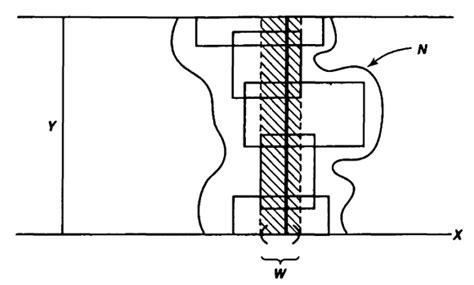
\includegraphics[scale=0.6]{lematubo.jpg}
    \label{fig:tubo}
    \end{figure}

    \hspace{0,5cm} \textit{Paso 2.} Sean $X$ e $Y$ compactos y $\mc{A}$ un recubrimiento abierto de $X \times Y$. Dado $x_0 \in X$, la rebanada $x_0 \times Y$ es compacta y estará recubierta por un n{\'u}mero finito de elementos $A_1, \ldots, A_m$ de $\mc{A}$. 
    
    La unión $\displaystyle N = \bigcup A_i$ es un abierto que contiene a $x_0 \times Y$, y por \textit{Paso 1}, el abierto $N$ contiene un tubo $W \times Y$ sobre $x_0 \times Y$ donde $W$ es abierto de $X$. Entonces $W \times Y$ está recubierto por un n{\'u}mero finito de $\{A_i\}$. 
    
    De esta forma, para cada $x \in X$, podemos elegir un $W$ tal que el tubo $W \times Y$ puede ser recubierto por elementos de $\mc{A}$ (de forma finita). La colección de todos los $W$ es recubrimiento de $X$. Por la compacidad de $X$, existe una colección finita de $W_i$ cubriendo a $X$. Por lo que la unión de los tubos 
    $$W_1 \times Y, \ldots, W_k \times Y$$
    es el espacio $X \times Y$, ya que cada uno puede ser cubierto por un n{\'u}mero finito de elementos de $\mc{A}$, de forma que $X \times Y$ es compacto. \hfill $\blacksquare$. 
    \item $\Leftarrow$) Definamos $\mathlarger{\mathlarger{\pi}}_X : X \times Y \longrightarrow X$ la proyección en $X$, continua y epiyectiva. Por lo visto en \hyperref[compapl]{\textcolor{blue}{\textbf{8.5. Compacidad por aplicaciones}}}, $Im \;  \mathlarger{\mathlarger{\pi}}_X = X$ es compacto. De manera similar se demuestra para $Y$.
\end{itemize}
\end{dem}
\begin{obs}
\textbf{Teorema de Tychonoff}. 
\begin{tcolorbox}
El producto infinito de compactos es un compacto. Para todo $X_i$ compacto, se cumple que: $$\mathlarger{\prod}_{i \in I}^{\infty} \; \mathlarger{X_i} \; \text{ es compacto}$$
\end{tcolorbox}
\end{obs}

\section{Compacidad en espacios m{\'e}tricos}
\begin{prop}
    Sea $(X,d)$ un espacio métrico, entonces el límite de una sucesión (si existe) es único.
\end{prop}
\begin{dem}
Supongamos que $\Lim{n}{\infty}{x_n}=x$ y $\Lim{n}{\infty}{x_n}=x$, entonces para cierto $n\in \mathbb{N}$ suficientemente grande se verificará que
$$d(x_n,x)<\varepsilon'$$
$$d(x_n,x')<\varepsilon''$$
para cualesquiera $\varepsilon',\varepsilon''>0$. Sumando ambas ecuaciones y aplicando la desigualdad triangular obtenemos que
$$d(x,x')\leq d(x_n,x)+d(x_n,x')<\varepsilon $$
luego necesariamente $x=x'$, ya que la distancia entre ambos puntos puede ser tan pequeña como se desee.



\end{dem}
\begin{teo}
Sea ($X,d$) un espacio m{\'e}trico,
\begin{tcolorbox}
\vspace{-4mm}
$$X \text{ es compacto } \Leftrightarrow \: X \text{ es compacto por sucesiones.}$$
\end{tcolorbox}
\end{teo}
\begin{dem} \: \vspace{-5mm}
\begin{itemize} 
    \item\justifying $\Rightarrow$) Sea $\{x_n\}$ una sucesión en $X$. Veamos que hay alguna subsucesión convergente. 
    $$S_1 = \{ x_1, \: x_2, \: x_3, \: \ldots \} \subseteq X$$
    $$S_2 = \{ x_2, \: x_3, \: x_4, \: \ldots \}$$
    $$\vdots$$
    $$S_k = \{ x_k, \: x_{k+1}, \: \ldots \}$$
    
    Veamos $\overset{\infty}{\underset{k=1}{\mathlarger{\bigcap}}} \: \overline{S_k}$ no es vacío. 
    Supongamos que fuera vacío, como $X$ es compacto, $\overline{S}_{k_1} \cap \ldots \cap \overline{S}_{k_r} = \emptyset$ donde $\overline{S}_{k_1} \cap \ldots \cap \overline{S}_{k_r} \supseteq S_{k_1} \cap \ldots \cap S_{k_r}=S_{k_j}$, (con $k_j = \max \{ k_1, \: \ldots, \: k_r\}$) pero $S_{k_j} = \{ x_{k_j}, \: x_{k_{j}+1}, \: \ldots 
    \} \neq \emptyset$, llegando a una contradicción.
    
    Luego existe $x \in \underset{k=1}{\overset{\infty}{\mathlarger{\mathlarger{}\bigcap}}} \: \overline{S_k}$ y además, $x \in \overline{S}_1$ . Entonces $\mc{B}(x,1) \cap S_1 \neq \emptyset$ son elementos de la sucesión, tales que existe $x_{n_1}$ que cumple $d(x, x_{n_1}) < 1$. De igual manera,
    $$x \in \overline{S}_{n_1 +1} \Longrightarrow \mc{B}(x, \nicefrac{1}{2}) \cap S_1 \neq \emptyset\Longrightarrow \exists\, x_{n_2}, \; d(x, x_{n_2}) < \frac{1}{2}$$
    $$x \in \overline{S}_{n_2 +1} \Longrightarrow  \mc{B}(x, \nicefrac{1}{3}) \cap S_1 \neq \emptyset \Longrightarrow \exists \,x_{n_3}, \; d(x, x_{n_3}) < \frac{1}{3}$$
    $$\vdots$$
    
    Continuando de manera sucesiva, de forma que $x_{n_1}, \; x_{n_2}, \; x_{n_3}, \; \ldots \; , x_{n_k}, \; \ldots $ es una subsucesión de $\{x_n\}$.
    
    Entonces $d(x, x_{n_k})<\nicefrac{1}{k} \; \Rightarrow \; \underset{k \to \infty}{\lim} d(x, x_{n_k}) = 0$. Entonces el límite de $x_{n_1}, \; x_{n_2}, \; x_{n_3}, \; \ldots \; , x_{n_k}, \; \ldots $ es $x$, es decir, dicha subsucesión converge a $x$.
    \item $\Leftarrow$) Sea $X=\underset{i}{\mbig[\bigcup}\: U_i$ un recubrimiento de $X$ por abiertos, hay que probar que un n{\'u}mero finito de $U_i$ recubre a $X$. Por el lema de Lebesgue, (se enuncia y demuestra más adelante), existe $\varepsilon > 0$ tal que para todo $x \in X$, $\mc{B}(x,\varepsilon)$ está centrada en alg{\'u}n $U_i$. Por el lema de acotación (se enuncia y demuestra más adelante), existe $x_1, \: \ldots, \: x_r \in X$ tales que $\mc{B}(x_1, \varepsilon) \cup \ldots \cup \mc{B}(x_r, \varepsilon) = X$ donde cada $\mc{B}(x_n, \varepsilon) \subseteq U_{i_n}$
\end{itemize}
\end{dem}

\textbf{Lema de Lebesgue.} Sea $X$ un espacio m{\'e}trico compacto por sucesiones y $X=\underset{i}{\mbig[\bigcup}\: U_i$ un recubrimiento de $X$ por abiertos
\begin{tcolorbox}Existe un $\varepsilon > 0$ tal que $\forall \: x \in X$, $\mc{B}(x,\varepsilon) \subseteq $ $U_i$ para algún $i$. A $\varepsilon$ se le denomina n{\'u}mero de Lebesgue del recubrimiento, y no es {\'u}nico, ya que si $\varepsilon$ lo cumple, $\nicefrac{\varepsilon}{2}$ tambi{\'e}n lo cumple.
\end{tcolorbox}
\begin{dem}
Supongamos que no existe ning{\'u}n $\varepsilon$ con esa propiedad, y por tanto, \\ 1 no es n{\'u}mero de Lebesgue. Esto es equivalente a que existe alg{\'u}n $x$ tal que $\mc{B}(x,1) \nsubseteq $ alg{\'u}n $U_i$. \\
$\nicefrac{1}{2}$ no es un nº de Lebesgue, luego existe alg{\'u}n $x$ tal que $\mc{B}(x,\nicefrac{1}{2}) \nsubseteq$ alg{\'u}n $U_i$.\\
De manera sucesiva, de forma que $\nicefrac{1}{n}$ no es un nº de Lebesgue, luego existe alg{\'u}n $x$ tal que $\mc{B}(x,\nicefrac{1}{n}) \nsubseteq$ alg{\'u}n $U_i$.\\
Tengamos una sucesión $\{ x_n \}$, sabiendo que $X$ es compacto por sucesiones, existe una subsucesión $\{ x_{n_k} \}$ convergente. Sea $x$ su límite, $x \in U_i$ para alg{\'u}n $i$ donde $\mc{B}(x,r) \subseteq U_i$. Tomemos un $k$ tal que 
$$\left\{ \begin{array}{l}
     x_{n_k} \in \mc{B}(x,r) \\
     \nicefrac{1}{n_k} < \nicefrac{r}{2} 
\end{array} \right.$$
Entonces, existe $\mc{B}(x_{n_k},\nicefrac{1}{n_k}) \subseteq \mc{B}(x,r)$, es decir, estamos haciendo bolas cada vez más ``pequeñas''. Cojamos $y \in \mc{B}(x_{n_k},\nicefrac{1}{n_k})$, observamos que
$$d(y, x_{n_k}) < \dfrac{1}{n_k} < \dfrac{r}{2}$$
Por tanto, 
$$d(y,x) \leq d(y, x_{n_k}) + d(x_{n_k}, x) < \dfrac{r}{2} + \dfrac{r}{2} = r$$
Se observa que $d(y,x) < r$ y por tanto, $y \in \mc{B}(x,r)$. Además, por hipótesis $\mc{B}(x,r) \subseteq U_i$, y por tanto $\mc{B}(x_{n_k}, \nicefrac{1}{n_k}) \subseteq U_i$. Lo cual es una \textcolor{red}{Contradicción}, rechazando la hipótesis y quedado demostrado la contraria. (Esto se debe a que al construir la subsucesión $\{ x_{n_k} \}$ existe un elemento tal que $\mc{B}(x_{n_k}, \nicefrac{1}{n_k})$ está contenida en algún $U_i$, luego $\frac{1}{n_k}$ sería un número de Lebesgue).
\end{dem}
\textbf{Lema de acotación.} 
\begin{tcolorbox}
Sea $X$ un espacio m{\'e}trico y compacto por sucesiones, sea $r>0$. Existe $x_1, \: \ldots, \: x_n$ tales que $\mc{B}(x_1, r) \cup \ldots \cup \mc{B}(x_n, r) = X$ (El espacio siempre se recubre por una unión finita de bolas de radio prefijado).
\end{tcolorbox}
\begin{dem}
Procederemos por reducción al absurdo. Supongamos que no podemos encontrar un nº finito de bolas que recubren a $X$. Sea $x_1 \in X$, $\mc{B}(x_1,r) \neq X$ (por la hipótesis, si un nº finito o recubre, una sólo, menos). \\
Por lo tanto, $x_2 \in X - \mc{B}(x_1,r)$, entonces $d(x_1, x_2) \geq r$. De esta forma, tenemos que $\mc{B}(x_1,r) \cup \mc{B}(x_2,r) \neq X$. Por lo que buscaremos un punto $x_3$ tal que su bola unión la anteriores sea el total, y así sucesivamente. Así, hemos construido una sucesión $x_1, \: x_2, \: x_3, \: \ldots, \: x_k, \: \ldots$ de forma que $d(x_i, x_j) > r \; \forall \: i<j$. \\
Al ser $X$ compacto por sucesiones, existe una subsucesión $\{ x_{n_k}\}$ convergente, de forma que $ ^{(1)} \; \: d(x_{n_i}, x_{n_j}) > r  \; \forall \: i<j$. Sea $x$ el límite de $\{ x_{n_k}\}$, existe un $k_0$ tal que 
$$d(x_{n_k},x)<\dfrac{r}{3} \; \; \text{ donde } k \geq k_0$$
Sean $k,k' \geq k_0$;
$$d(x_{n_k}, x_{n_{k'}}) \leq d(x_{n_k}, x) + d(x, x_{n_{k'}}) < \dfrac{r}{3} + \dfrac{r}{3}<r$$
Usando $^{(1)}$, llegamos a una \textcolor{red}{Contradicción} con lo anterior, y por tanto, rechazando la hipótesis que supusimos y demostrando lo contrario.
\end{dem}
Sea $(X,d)$ un espacio m{\'etrico}, 
\begin{teox}
De manera  alternativa, podemos realizar la demostración del teorema demostrando que las siguientes afirmaciones son equivalentes: \vspace{-2mm}
\begin{enumerate}[1)]
    \item $X$ es compacto
    \item $X$ es compacto por punto límite
    \item $X$ es compacto por sucesiones
\end{enumerate}
Lo que nos interesa en este caso es que 1) $\Rightarrow$ 2) $\Rightarrow$ 3) para demostrar la implicación directa del Teorema. La demostración de que 3) $\Rightarrow$ 1) es la expuesta previamente.
\end{teox}
\begin{demx}
Ya hemos demostrado que 1) $\Rightarrow$ 2) (en \hyperref[lim]{\textcolor{blue}{\textbf{8.3.}}}), veamos que 2) $\Rightarrow$ 3). Comenzamos por suponer que $X$ es compacto por punto límite. Dada una sucesión ($x_n$) de puntos de $X$, consideremos el conjunto $A=\{x_n \: / \: n \in \mathbb{Z_+}\}$. Si el conjunto $A$ es finito, entonces existe un punto $x$ tal que $x=x_n$ para un n{\'u}mero infinito de valores de $n$. En este caso, la sucesión ($x_n$) tiene una subsucesión que es constante y, por tanto, converge. Por otro lado, si $A$ es infinito, entonces $A$ tiene un punto límite $x$. Definamos una subsucesión de $(x_n)$ convergente a $x$ del siguiente modo: 

Elegimos $n_1$ tal que 
$$x_{n_1} \in \mc{B}(x,1)$$

Supongamos entonces que el entero positivo $n_{i-1}$ está dado, por lo que la bola $\mc{B}(x, 1/i)$ intersecta a $A$ en un n{\'u}mero finito de puntos. Así pues, elegimos un índice $n_i > n_{i-1}$ tal que 
$$x_{n_i} \in \mc{B}(x, 1/i)$$
Entonces la subsucesión $x_{n_1}, x_{n_2}, \ldots $ converge a $x$.
\end{demx}
\chapter{ESPACIOS M{\'E}TRICOS COMPLETOS}
\section{Sucesiones de Cauchy y completitud}
Sea $(X,d)$ un espacio m{\'e}trico
\begin{defi} 
Una sucesión $\{ x_n \}$ se dice que es una \textbf{sucesión de Cauchy} si tiene la propiedad de que, dado un $\varepsilon > 0$, existe un entero $k$ tal que:
$$d(x_k, x_n) < \varepsilon \qquad \forall \; n \geq k$$
Equivalentemente, podemos dar la siguiente definición: para todo $\varepsilon > 0 \:$ existe $ \: k \: $ tal que $ \: d(x_n,x_m) <  \varepsilon \: \forall \: n,m \geq k$

\end{defi}
\begin{prop}
Si $\{ x_n \}$ es convergente, entonces es de Cauchy.
\end{prop}
\begin{dem}
Sea $x$ el límite de la sucesión, sea $\varepsilon > 0$, existe $k$ tal que $d(x_k, x) < \nicefrac{\varepsilon}{2} \; \forall \: n \geq k$. Por tanto, si $n \geq k$,
$$d(x_k, x_n) \leq d(x_k, x) + d(x,x_n) < \dfrac{\varepsilon}{2} +\dfrac{\varepsilon}{2} = \varepsilon$$
Por tanto, concluimos que toda sucesión convergente es una sucesión de Cauchy.
\end{dem}
\begin{obs}
No tiene por qu{\'e} cumplirse el recíproco. De hecho, si se cumple, tenemos el siguiente tipo de espacios:
\end{obs}
\begin{lem}\; 
\begin{tcolorbox}
Un espacio m{\'e}trico $X$ es \textbf{completo} si toda sucesión de Cauchy es convergente.
\end{tcolorbox}
\end{lem}
\begin{eje}
$\mathbb{R}$ es completo. $\mathbb{R}^k$ también. 
\end{eje}
\begin{obs}

Sean $X$ e $Y$ dos espacios m{\'e}tricos con sus respectivas ditancias $d_X$ y $d_Y$, el espacio $X \times Y$ tambi{\'e}n es m{\'e}trico, con la distancia $d_{\infty}$ definida por: $d_{\infty}(z,z')=\max\{d_X(x,x'), d_Y(y,y')\}$ donde $z = (x,y)\in X \times Y$ y $z' = (x',y')\in X \times Y$

\end{obs}
\begin{prop} \; 
\vspace{-3mm}\begin{center}
    $X$ e $Y$ son completos $\Leftrightarrow$ $X \times Y$ es completo.
\end{center}
\end{prop}
\begin{dem} \;
\justifying

\vspace{-3mm}$\Rightarrow$) Sea $\{z_n\}$ una sucesión de Cauchy en $X \times Y$, cada $z_n=(x_n, y_n)$. Veamos que 
\begin{addmargin}[1,7em]{0em}\begin{enumerate}[1)]
    \item $\{x_n\}$ es una sucesión en $X$, que al ser $X$ completo, converge a alg{\'u}n $x \in X$, y por tanto, es de Cauchy.
    \item $\{y_n\}$ es una sucesión de Cauchy en $Y$, ya que, de manera análoga al anterior, converge a un $y \in Y$. 
\end{enumerate}
\end{addmargin}
Por lo tanto, $\{z_n\}$ converge a $z=(x,y)$. Probemos que se cumple 1). Sea $\varepsilon > 0$ y $\{z_n\}$ de Cauchy, existe $k>0$ tal que:
$$d_X(x_k,x_n) \stackrel{*}{\leq} d_{\infty}(z_k,z_n) < \varepsilon \; \; \;  \forall \: n \geq k$$
$(^*)$ por la definición de $d_{\infty}$, ya que se cumple siempre que el máximo de dos elementos es mayor o igual que cualquiera de ellos. Por lo tanto, se comprueba que $x_n$ es de Cauchy y por el mismo razonamiento se demuestra 2).

 Probemos ahora que $\{z_n\}$ converge a $z=(x,y)$.
$$d(z_n,z)=\max\{\underbrace{d_X(x_n,x)}_{\stackrel{n \to \infty}{\longrightarrow} 0}, \underbrace{d_Y(y_n,y)}_{\stackrel{n \to \infty}{\longrightarrow} 0}\}=0 \; \Rightarrow \; z \text{ es el límite de } z_n$$

$\Leftarrow$) Sea $y \in Y$, podemos definir 
$$i: X \times \{y\} \hookrightarrow X \times Y$$
donde $\{y\}$ es un cerrado, y por tanto, $X \times \{y\}$ es cerrado (ya que cerrado $\times$ cerrado = cerrado). $X$ se puede identificar con un cerrado de $X\times Y$ ($X \times \{y\}$), donde a cada $x$ se le asigna $(x,y)$ con $y$ fijo. Al ser $X$ cerrado de $X \times Y$, que es completo, $X$ también lo será (ver una de las proposiciones posteriores).
\end{dem}
\section{Subespacios completos}
\begin{prop}
Sean $\{ x_n \},\: \{ y_n \} $ dos sucesiones de Cauchy en un espacio métrico $X$ y $a_n=d(x_n,y_n)$, luego $\{ a_n \}$ es una sucesión de n{\'u}meros reales (donde todos son $>$ 0). Entonces, $\{ a_n \}$ es una sucesión de Cauchy de n{\'u}meros reales.
\end{prop}
\begin{dem}
Dado un $\varepsilon > 0$, tenemos que ver que existe $k$ tal que $|a_k - a_n| < \varepsilon \; \forall \; n \geq k$. Como $\{ x_n \},\: \{ y_n \}$ son de Cauchy, existen $k_1,k_2$ que cumplen:
$$d(x_n,x_m) < \dfrac{\varepsilon}{2} \qquad d(y_n,y_m) < \dfrac{\varepsilon}{2} \qquad \qquad \forall \; n,m \geq k_1,k_2$$
De esta forma, tomando $k=\max\{k_1,k_2\}$:
$$a_n = d(x_n,y_n) \leq \underbrace{d(x_n,x_k)}_{< \: \nicefrac{\varepsilon}{2}} + \underbrace{d(x_k,y_k)}_{= \: a_k}+ \underbrace{d(y_k,y_n)}_{< \: \nicefrac{\varepsilon}{2}}< \nicefrac{\varepsilon}{2}+d(x_k,y_k)+\nicefrac{\varepsilon}{2}=a_k+\varepsilon$$
Recolocando la expresión anterior, tenemos que $\boxed{a_n < a_k + \varepsilon}$.\\  Podemos intercambiar $n$ por $k$, y repitiendo el argumento anterior, obtendríamos $\boxed{a_k < a_n + \varepsilon}$. De forma que $$a_n \in (a_k-\varepsilon, \: a_k+ \varepsilon) \; \Rightarrow \; a_k + \varepsilon < a_n < a_k + \varepsilon \; \Rightarrow \; |a_n - a_k | < \varepsilon$$
Luego se demuestra que es convergente, y por tanto, de Cauchy, luego es convergente. .
\end{dem}
\begin{cor}
    Existe $\displaystyle \lim_{n \to \infty}d(x_n,y_n) \in \mathbb{R}$    
\end{cor}
\begin{prop}Sea $X$ un espacio m{\'e}trico completo y $S \subseteq X$ un subespacio, \vspace{-5mm}
\begin{center}
    $S$ es completo $\Leftrightarrow$ $S$ es un cerrado de $X$
\end{center}
\end{prop}
\vspace{-5mm}
\begin{dem} \: 
\justifying

$\Leftarrow$) 
Supongamos que $S$ es un cerrado de $X$, veamos que es completo. Sea $\{s_n\}$ una sucesión de Cauchy en $S$, lo que implica que es una sucesión de Cauchy en $X$. Al ser $X$ completo, $\{s_n\}$ converge a un punto $x \in X$. Entonces $x$ es adherente a $\{s_n\}$ por definición. Por lo tanto, es adherente a $S$ y por ser $S$ cerrado, $x \in S$. Por lo tanto, $\{ s_n \}$ es convergente en $S$, y por tanto, $S$ es completo.

$\Rightarrow$) Suponiendo que $S$ es completo, veamos que es cerrado. Sea $x \in \overline{S}$, veamos que $x \in S$.\\
Para cada $n \in \mathbb{N}$, existe $s_n \in S$ tal que $d(x, s_n) < \nicefrac{1}{n}$. Tenemos por tanto $\{s_n\}$ una sucesión en $S$, que converge a $x$. Entonces $\{s_n\}$ es una sucesión convergente (en $X$), y por tanto, es de Cauchy. Luego $\{s_n\}$ es una sucesión de Cauchy en $S$. Al ser $S$ completo, la sucesión es convergente en $S$, con límite $x$, y por tanto, $x \in S$, quedando así demostrada la proposición.
\end{dem}

\section{Completación}
\begin{defi}
Sean $\{ x_n \},\: \{ y_n \} $ dos sucesiones de Cauchy en $X$, entonces $\mathlarger{\exists} \; \underset{n \to \infty}{\lim} \; d(x_n, y_n)$. Definimos pues la siguiente relación de equivalencia:
$$\{ x_n \} \: \sim \: \{ y_n \} \text{ \; si \; } \underset{n \to \infty}{\lim} \; d(x_n, y_n)=0$$ 
\end{defi}
\begin{nota}
Denotamos:
$$\mathlarger{\mathlarger{\hat{X}}}=\mathlarger{\mathlarger{\nicefrac{\{ \text{Sucesiones de Cauchy en } X\}}{ \sim }}}$$
donde sus elementos son $\hat{x} \in \hat{X}$ tal que $\hat{x}=[\{x_n\}]$. De esta forma, si dos elementos están relacionados, sus clases son la misma, es decir $[\{x_n\}] = [\{y_n\}] \: \Leftrightarrow \: \{x_n\} \sim \{y_n\}$.
\end{nota}
\begin{obs}
Dotaremos a $\hat{X}$ de estructura de espacio métrico considerando la siguiente distancia: 
$$\hat{d}(\hat{x}, \hat{y}) := \underset{n \to \infty}{\lim} d(x_n, y_n)$$
\end{obs}
\textbf{Ejercicio:} Probar que es una distancia. Para ello, probar que está bien definida respecto a las clases de equialencia y que cumple las propiedades definidas en \hyperref[dist]{\textcolor{blue}{\textbf{1.2. Espacios m{\'e}tricos}}} (definida positiva, simétrica y que cumple la desigualdad triangular).

Para ver que está bien definida respecto a las clases de equivalencia, veamos no depende del representante elegido. Consideremos dos sucesiones relacionadas $\{x_n\} \sim \{x_n'\}$, y comprobemos que $$\hat{d}(\hat{x}, \hat{y})=\hat{d}([\{x_n\}], [\{y_n\}])=\lim_{n \to \infty} d(x_n,y_n)=\lim_{n \to \infty} d(x_n',y_n')=\hat{d}([\{x_n'\}], [\{y_n'\}])$$
\begin{eje}
Si $X= \mathbb{Q}$, $\hat{\mathbb{Q}}= \mathbb{R}$.
\end{eje}
\begin{defi} \justifying
A $\hat{X}$ lo llamamos \textbf{completación} (o complección) de $X$. Además, se tiene que $X\subseteq \hat{X}$. Dado $x \in X$, sea $\{ x_n \}$ una sucesión tal que $\; x_n = x \; \forall \: n$. Definimos la inclusión de la forma:
$$\begin{array}{rcl}
     X & \stackrel{i}{\longrightarrow} & \hat{X} \\
     x & \longmapsto & i(x) = [\{ x_n \}] (x_n=x) 
\end{array}$$
ya que es convergente, luego de Cauchy por tanto nos da una clase de equivalencia.
\end{defi}
\begin{obs}
    Esta aplicación $i$ es la que usamos usualmente para incluir $\mathbb{Q}$ en $\mathbb{R}$, de forma que asignamos a cada $q \in \mathbb{Q}$ la sucesión constante $x_n = q \: \forall n$.
\end{obs}
\begin{prop}
$i$ es una isometría, es decir, $d(x,y)=\hat{d}(i(x), i(y))$.
\end{prop}
\begin{dem} V{\'e}ase la siguiente cadena de igualdades:
$$\hat{d}\big(i(x), i(y)\big)=\hat{d}\big([\{ x_n \}], [\{ y_n \}]\big) = \underset{n \to \infty}{\lim} d(x_n,y_n) = \underset{n \to \infty}{\lim} d(x,y)=d(x,y)$$

\end{dem}
\vspace{3mm}
\begin{tcolorbox}
\begin{lem} $X$ es denso en $\hat{X}$, es decir, la aplicación $i$ es densa \Big($\overline{i(X)} = \hat{X}$\Big). \end{lem}
\end{tcolorbox}

\begin{dem}
Veamos que todo punto de $\hat{X}$ es adherente a $i(X)$. Sea $\hat{x} \in \hat{X}$, tenemos que comprobar que $\forall \: \varepsilon > 0$ se cumple que $\mc{B}(\hat{x}, \varepsilon) \cap i(X) \neq \emptyset$. Sabemos que $\hat{x}=[\{x_n\}]$, por tanto, existe un $k$ tal que $d(x_k,x_n) < \nicefrac{\varepsilon}{2} \; \forall \: n \geq k$. Usando la definición de $\hat{d}$:
$$\hat{d}(i(x_k), \hat{x}) < \varepsilon \; \Rightarrow \; i(x_k) \subset \mc{B}(\hat{x}, \varepsilon)$$
\end{dem}
Demostraremos un Lema que utilizaremos en la demostración de que $\hat{X}$ es completo.
\begin{lem}
Sea $X$ un espacio m{\'e}trico y $S \subseteq X$ un subespacio denso, 
\begin{tcolorbox}
Si toda sucesión de Cauchy en $S$ es convergente en $X$, entonces $X$ es completo.
\end{tcolorbox}

\end{lem}
\begin{dem}
Sea $\{x_n\}$ una sucesión de Cauchy en $S$, tenemos que ver que es convergente. Como $S$ es denso, existe $s_n \in S \: : \: d(s_n,x_n) < \nicefrac{1}{n}$
\begin{enumerate}[1)]
    \item $\{s_n\}$ es de Cauchy
    \begin{dem}
    Dado $\varepsilon > 0$, existe $k$ tal que $d(s_k,s_n) < \varepsilon \; \forall \: n \geq k$
    $$d(s_k,s_n)\leq \underbrace{d(s_k,x_k)}_{< \: \nicefrac{1}{k} \: \stackrel{*}{<} \: \nicefrac{\varepsilon}{3}} + \underbrace{d(x_k,x_n)}_{< \: \nicefrac{\varepsilon}{3}} + \underbrace{d(x_n,s_n)}_{< \: \nicefrac{1}{n}\: \leq \: \nicefrac{1}{k} \: \stackrel{*}{<} \: \nicefrac{\varepsilon}{3}} < \varepsilon$$
    * se cumple para $k>>0$, es decir, para un $k$ lo suficientemente grande.
    
    Por tanto, $x \in X$ es límite de $\{ s_n \}$ 
    \end{dem} 
    \item $\{s_n\}$ tiene límite en $X$
    \begin{dem}
    Por ser $S$ denso, todo punto de $X$ es adherente a $S$ y, por tanto, $\Lim{n}{\infty}{s_n}=x\in X$
    \end{dem}
    \item $x$ es límite de $\{x_n\}$
    \begin{dem}
    Veamos si se cumple $ \underset{n \to \infty}{\lim} d(x_n,x) = 0$
    $$d(x_n, x ) \stackrel{*}{\leq} \underbrace{d(x_n,s_n)}_{< \: \nicefrac{1}{n}} + \underbrace{d(s_n,x)}_{ 0 \: (n \to \infty) } $$
    * se ha usado la desigualdad triangular. Por tanto, $\Lim{n}{\infty}{d(x_n,x)}=0$, quedando demostrado el lema.
    \end{dem}
\end{enumerate}
\end{dem}
\begin{tcolorbox}
    \begin{teo} $\hat{X}$ es completo.\end{teo}
\end{tcolorbox}
\begin{dem}
Sabemos que $X$ está contenido en $\hat{X}$, es decir, $X \stackrel{i}{\hookrightarrow} \hat{X}$. Por el lema anterior, basta probar que toda sucesión de Cauchy en $i(X)$ es convergente en $\hat{X}$.

Sea $\{x_n\}$ una sucesión de Cauchy en $X$, veremos que $\{i(x_n)\}$ converge en $\hat{X}$. Sea $\hat{x}=[x_n]$, demostremos que la sucesión $\{i(x_n)\}$ converge a $\hat{x}$.

Dado $\varepsilon>0$, por ser $x_n$ de Cauchy sabemos que existe $N\in\mathbb{N}$ tal que si $n,m\geq N$ entonces $d(x_n,x_m)<\varepsilon$. En particular, para cada $m\geq N$ se tiene que $d(x_n,x_m)<\varepsilon$ para todo $n\geq N$, con lo cual, si $m\geq N$ se tiene que:
$$\hat{d}(\hat{x},i(x_m))=\Lim{n}{\infty}{d(x_n,x_m)}<\varepsilon$$
luego $i(x_n)$ converge a $\hat{x}$.

ver que $\hat{d}\big(i(x_k), \hat{x}\big) \underset{k \to \infty}{\longrightarrow}  0$, donde $i(x_k)=[\{y_n\}]$ es la sucesión constante $x_k$ y $\hat{x}=[\{x_n\}]$:
$$\hat{d}\big(i(x_k), \hat{x}\big) = \underset{n \to \infty}{\lim} d(y_n,x_n)=\underset{n \to \infty}{\lim} d(x_k,x_n) \stackrel{*}{<} \varepsilon$$
* para $k >> 0$ y $n \geq k$, $d(x_k,x_n) < \varepsilon$ porque $\hat{d}\big(i(x_k), \hat{x}\big) < \varepsilon$. \hfill $\square$
\end{dem}

\begin{prop}
Sea $f: X \longrightarrow Y$ una isometría,
\vspace{-4mm}\begin{center}
    Existe una {\'u}nica isometría entre la completación de los espacios $\hat{f}: \hat{X} \longrightarrow \hat{Y}$.
\end{center}
\end{prop}

\begin{obs}
Como hemos visto, podemos definir las inclusiones $i_X: X {\hookrightarrow} \hat{X}$ y $i_Y: Y {\hookrightarrow} \hat{Y}$, creando el siguiente diagrama (que será conmutativo si se cumple la proposición):
 $$\begin{tikzcd}
     X  \arrow[hookrightarrow]{d}{i_X} \arrow{r}{f} & Y \arrow[hookrightarrow]{d}{i_Y} \\
     \hat{X} \arrow{r}{\hat{f}} & \hat{Y}
 \end{tikzcd} $$
\end{obs}

\begin{dem}
\underline{Existencia.}

Sea $\{x_n\}$ una sucesión de Cauchy en X, entonces $\{f(x_n)\}$ es una sucesión de Cauchy en $Y$ (por ser $f$ una isometría). \\
Si $\{x_n\} \: \sim \: \{x_n'\}$, entonces $\{f(x_n)\} \: \sim \{f(x_n')\}$ (por ser $f$ una isometría).
Definimos:\\ $$\begin{array}{rccl}
     \hat{f}: & \hat{X} & \longrightarrow & \hat{Y}  \\
     \; & \hat{x}= [\{x_n\}] & \longrightarrow & \hat{f}(\hat{x}):=[\{f(x_n)\}]
\end{array} $$
Veamos que $\hat{f}$ es una isometría. Comprobemos que 
$$\hat{d}_X(\hat{x}, \hat{x}') = \hat{d}_Y(\hat{f}(\hat{x}),\hat{f}(\hat{x'}))$$
donde $\hat{x}=[\{x_n\}]$ y $\hat{x}'=[\{x_n'\}]$. La distancia $\hat{d}$ se define como:
$$\hat{d}_X(\hat{x},\hat{x}')=\lim_{n \to \infty} d_X(x_n, x_n')=\lim_{n \to \infty} d_Y\big(f(x_n), f(x_n')\big)=\hat{d}_Y([\{f(x_n)\}], [\{f(x_n')\}])=\hat{d}_Y(\hat{f}(\hat{x}), \hat{f}(\hat{x}'))$$
Se ve de forma inmediata que el diagrama observado previamente es conmutativo, comprobándose que $i_Y \circ f = \hat{f} \circ i_X$, apliquemos ambas composciones a un $x \in X$:
$$(i_Y \circ f)(x)=i_Y(f(x))=[\{\text{\textit{sucesión cte.}}=f(x)\}]$$
$$(\hat{f} \circ i_X)(x)=\hat{f}(i_X(x))=\hat{f}([\{x_n\}])=\hat{f}(\hat{x})=[\{f(x_n)\}]\stackrel{(1)}{=}[\{f(x)\}]$$
$^{(1)}$ todos los $x_n=x$, es decir, la sucesión constante. \\ 
Cumpli{\'e}ndose así la igualdad, y por tanto, la existencia de la isometría $\hat{f}$.

\underline{Unicidad.}
Sea $\widetilde{f}: \hat{X} \longrightarrow \hat{Y}$ una isometría tal que $i_Y \circ f = \widetilde{f} \circ i_X$. Veamos que $\hat{f}=\widetilde{f}$. Uniendo las expresiones de los diagramas, tenemos que $\widetilde{f} \circ i_X = \hat{f} \circ i_X$. Es decir, $\hat{f}$ y $\widetilde{f}$ coinciden sobre $i_X(x)$, es decir, que $\hat{f}$ y $\widetilde{f}$ coinciden sobre $\overline{i_X(x)} = \hat{X}$. Con el siguiente lema, concluiremos la demostración:
\end{dem}

\begin{lem}
Sean $X \underset{g}{\overset{f}{\rightrightarrows}} Y$ dos aplicaciones continuas y sea $S=\{ x \in X \: / \: f(x)=g(x) \} \subseteq X$ \vspace{-3mm} 
\begin{tcolorbox}
\begin{center}
    Si $Y$ es separado ($T_2$), entonces $S$ es un cerrado de $X$.
\end{center}
\end{tcolorbox}
\end{lem}
\begin{dem}
Definamos la aplicación producto:
$$\begin{array}{rrcl}
     f \times g : & X & \longrightarrow & Y \times Y \\
     \: & x & \longmapsto & (f \times g)(x):=(f(x), g(x))
\end{array}$$
De forma que la diagonal $\Delta = \{y,y\} \subseteq Y \times Y$ es un cerrado de $Y \times Y$ por ser $Y$ separado. Por tanto, $$S=\{ x \in X \: / \: f(x)=g(x) \}=\big\{ x \in X \: / \: \big(f(x),g(x)\big) \in \Delta \big\} = (f \times g)^{-1}(\Delta)$$ 
donde $(f \times g)^{-1}(\Delta)$ es cerrado de $X$.

Quedando demostrada así la unicidad, y por tanto, la proposición. \hfill $\square$
\end{dem}\label{densaplic}

\begin{prop} Sea $X$ un espacio m{\'e}trico e $i: X \hookrightarrow \hat{X}$,
\vspace{-4mm}\begin{center}
    $X$ es completo $\Leftrightarrow$ $i$ es un homeomorfismo
\end{center}
\end{prop}
\begin{dem} \:
\justifying

$\Rightarrow$) Que $X$ sea completo implica que $i(x)$ es un subespacio completo de $\hat{X}$, y al mismo tiempo, que $i(x)$ es un cerrado de $\hat{X}$ y que $\overline{i(x)}=i(x)$. A su vez, $\overline{i(x)}=\hat{X}$. Demostrando así que es un homeomorfismo.

$\Leftarrow$) Siendo $i$ un homeomorfismo, como $\hat{X}$ es completo, por definición de isometría y homeomorfismo, $X$ es completo. \hfill $\square$
\end{dem}
\begin{prop}
    Sean $X,Y$ espacios m{\'e}tricos completos, existe una {\'u}nica isometr{\'i}a $\hat{f}$ tal que $\hat{f} \circ i = f$, es decir, tal que el siguiente diagrama es conmutativo:
    $$\begin{tikzcd}
     X \arrow[hook]{r}{i} \arrow{d}{f} & \arrow[dotted]{dl}{\hat{f}} \hat{X} \\
     Y & 
\end{tikzcd}$$
\end{prop}
\begin{dem}
\underline{Existencia:}\\
Definimos la siguiente aplicación:
$$\begin{array}{rccl}
     \hat{f}: & \hat{X} & \longrightarrow & Y  \\
     \; & \hat{x} & \longrightarrow & \hat{f}(\hat{x}):=f(x)
\end{array} $$
donde $[x]=\hat{x}$. Veamos que esta aplicación está bien definida, esto es, que no depende del representante de la clase de equivalencia elegido. Si $[x]=[y]=\hat{x}$, entonces $\hat{f}(\hat{x})=f(x)=f(y)$ y por ser $f$ isometría será inyectiva, luego necesariamente $x=y$.

Ahora comprobaremos que es en efecto una isometría:
$$\hat{d}(\hat{x},\hat{y})=\Lim{n}{\infty}{d_X(x_n,y_n)}=\Lim{n}{\infty}{d_Y(f(x_n),f(y_n))}=\Lim{n}{\infty}{d_Y(\hat{f}([x_n]),\hat{f}([y_n]}))=\hat{d}(\hat{f}(\hat{x}),\hat{f}(\hat{y}))$$
\end{dem}
\begin{propx} \:
\vspace{-7mm}\begin{center}
    $X$ es compacto $\Leftrightarrow$ $\mathlarger{\mathlarger{\pi}}_T$ es cerrada
\end{center}
\end{propx}
\begin{demx} \;

$\Rightarrow$) Sea $C$ un cerrado de $X \times T$, veamos que $\mathlarger{\mathlarger{\pi}}(C)$ es un cerrado de $T$, es decir, que $T-\mathlarger{\mathlarger{\pi}}(C)$ es abierto. 

Sea $t \in T-\mathlarger{\mathlarger{\pi}}(C)$, existe un abierto $V_t$ con $t \in V_t$ y $V_t \subseteq T-\mathlarger{\mathlarger{\pi}}(C)$ (un \textcolor{blue}{entorno de $t$}). Tengamos que $t \in T-\mathlarger{\mathlarger{\pi}}(C) \equiv \mathlarger{\mathlarger{\pi}}^{-1}(t) \cap C \neq \emptyset$ donde $X \times \{t\} = \mathlarger{\mathlarger{\pi}}^{-1}(t)$. Para cada $x \in X$ que no pertenezca a $C$, existen abiertos $U_x \times V_t^{x}$ de modo que $(x,t) \in U_x \times V_t^{\times}$ no corta a $C$. 

El conjunto $\{U_x\}_{x \in X}$ recubre a $X$ (compacto). De forma que podemos relacionar cada $U_{x_i} \longleadsto{0.3} V_t^{x_i}$, asegurando que $\{V_t^{x_i}\}_{i \in I}$ recubre a $X$.

Sea $V_t=V_t^{x_1} \cap \ldots \cap V_t^{x_n}$ abierto que contiene a $t$, veamos que $V_t$ no corta a \\ $\mathlarger{\mathlarger{\pi}}(C)=\mathlarger{\mathlarger{\pi}}^{-1}(V_t)$, que no corta a $C$, donde 
$$\mathlarger{\pi}^{-1}(V_t)=(X \times V_t)=(U_{x_1} \times V_t) \cup \ldots \cup (U_{x_n} \times V_t)$$
donde cada ``unionando'' no corta a $C$, y por tanto, $V_t$ tampoco ($V_t \cap C = \emptyset$). Demostrando así que si $X$ es compacto, $\mathlarger{\pi}_T$ es cerrada $\forall \; T$.

$\Leftarrow$) Sea $C$ un cerrado tal que $C \subseteq X \times T$, sea $t \in \mathlarger{\mathlarger{\pi}}(C) \equiv \mathlarger{\mathlarger{\pi}}^{-1}(t) \cap C = \emptyset$ y además, $U_t \cap \mathlarger{\mathlarger{\pi}}(C)=\emptyset \equiv \mathlarger{\mathlarger{\pi}}^{-1}(U_t) \cap C = \emptyset$ donde $t \in U_t$, llegando a una \textcolor{red}{contradicción !!}
\end{demx}

\chapter{HOMOTOPÍA}
\begin{defi}
Dos aplicaciones continuas $f, g :  X \longrightarrow Y$ son \textbf{homótopas} si existe otra aplicación continua $H: I=[0,1] \times X \longrightarrow Y$ tal que:
$$H(0,x) = f(x)$$
$$H(1,x) = g(x)$$
Dado $t \in I$, se tienen las aplicaciones $H_t: X \longrightarrow Y$ definidas por $H_t(x):=H(t,x)$.
\end{defi}

\begin{obs}
Podemos entender una homotopía como una familia uniparamétrica continua de aplicaciones de $X$ en $Y$. Si el parámetro $t$ representa un tiempo, una homotopía describe una deformación continua de $f$ en $g$ cuando el tiempo recorre el intervalo $I$.
\end{obs}

Sean $\gamma, \gamma': [0,1] \longrightarrow X$ dos caminos en $X$ con $\gamma(0)=\gamma'(0)$ y $\gamma(1)=\gamma'(1)$, es decir, con el mismo inicio y final.
\begin{defi} \label{camhom}
Dados $\gamma$ y $\gamma'$, diremos que esos dos caminos son \textbf{homótopos} ($\gamma \sim \gamma'$) si existe $H: I \times I \longrightarrow X$ que cumple:
\begin{enumerate}
    \item $H(0,s) = \gamma(s)$ y $H(1,s) = \gamma'(s) \; \forall s \in I$, es decir, $H_0=\gamma,\; H_1=\gamma'$.
    \item Para cada $t \in I, \; H_t: I \longrightarrow X$ tiene el mismo origen y final que $\gamma$ y $\gamma'$\\($\gamma(0)=\gamma'(0)=H_t(0)$ y $\gamma(1) = \gamma'(1) = H_t(1)$).
\end{enumerate}
\end{defi}
\begin{figure}[h]
    \centering
    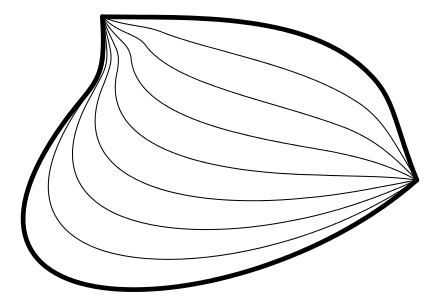
\includegraphics[scale=0.3]{homotopia.png}
    \caption{Los caminos en negrita son los caminos $\gamma$ y $\gamma'$ y los ``intermedios'' los $H_t$}
    \label{fig:homotopia}
\end{figure}
\begin{obs}
Tenemos un camino para cada $t$, de forma que siempre están entre $\gamma$ y $\gamma'$, obteniendo así caminos ``intermedios'' entre ellos, es decir, $\gamma$ se deforma a $\gamma'$. Diremos que $H$ es la homotopía de caminos que transforma $\gamma$ en $\gamma'$.
\end{obs}
\begin{nota}
Denotaremos por $H^{t'}(t)=H(t,t')$ (igual que denotamos por $H_t(t')=H(t,t')$) aunque no la usaremos.
\end{nota}
\begin{propi}
$\sim$ es una relación de equivalencia, de forma que cumple:
\vspace{-3mm}\begin{enumerate}
    \item Reflexiva: $\gamma \sim \gamma$ 
    \begin{dem}
    Tomemos $H$ tal que $H_t = \gamma$ para todo $t$, entonces $H_0 = H_1 = \gamma$ y $H_t(0) = \gamma(0),\,H_t(1) = \gamma(1)$.
    \end{dem}
    \item Sim{\'e}trica: $\gamma \sim \gamma' \Leftrightarrow \gamma' \sim \gamma$ 
    \begin{dem}
    Sea $H$ la homotopía de la primera relación. Definimos $H'$ tal que $H'_t=H_{1-t}$. Tenemos que $H'(t,t')=H_t'(t')=H_{1-t}(t')=H(1-t,t')$. De esta forma, $H_0'=H_1=\gamma'$ y $H_1'=H_0=\gamma$. Además, $H'_t(0) = H_{1-t}(0) = \gamma(0) = \gamma'(0)$, y $H'_t(1) = H_{1-t}(1) = \gamma(1) = \gamma'(1)$.
    \end{dem}
    \item Transitiva Si $\gamma \sim \gamma'$ y $\gamma' \sim \gamma'' \; \Rightarrow \; \gamma \sim \gamma'' $
    \begin{dem}
    Utilizamos $H$ y $H'$ como en la propiedad anterior, definimos \\ \vspace{3mm} \hspace{5mm} $H''(t,t')=\left\{ \begin{array}{ll}
         H(2t,t') & \text{ si } 0 \leq t \leq \nicefrac{1}{2}  \\
         H'(2t-1,t') & \text{ si } \nicefrac{1}{2} \leq t \leq 1 
    \end{array} \right.$\\ \vspace{2mm}
    Veamos que sucede con $t=\nicefrac{1}{2}$:\\ \vspace{2mm}
    \hspace{5mm} $t=\nicefrac{1}{2}:=\left\{ \begin{array}{l}
        H(1,t')=H_1(t)=\gamma(t')  \\
        H'(0,t')=H_0'(t')=\gamma'(t') 
    \end{array} \right.$    \\ \vspace{2mm}
    Podemos definir por tanto: \\ \vspace{2mm}
    \hspace{5mm}  $H''_t = \left\{ \begin{array}{ll}
        H_{2t}  & \text{ si } 0 \leq t \leq \nicefrac{1}{2} \\
        H_{2t-1}& \text{ si } \nicefrac{1}{2} \leq t \leq 1
    \end{array} \right.$
    \end{dem} 
\end{enumerate}
\end{propi}
Ya que $\sim$ es una relación de equivalencia, definimos $[\gamma] = \{\gamma' \; / \; \gamma \;\sim\; \gamma'\}$. Con esto, la operación suma de caminos induce una operación sobre las clases de homotopía de caminos, dada por: $$[\gamma_1] \cdot [\gamma_2] = [\gamma_1 \cdot \gamma_2]$$

\begin{prop}
Esta operación está bien definida.
\end{prop}
\begin{dem}
Sean $\gamma_1' \in [\gamma_1],\, \gamma_2' \in [\gamma_2]$, y sea $F$ una homotopía entre $\gamma_1$ y $\gamma_1'$, y $G$ una entre $\gamma_2$ y $\gamma_2'$. Debemos comprobar que $(\gamma_1' \cdot \gamma_2') \;\sim\; (\gamma_1 \cdot \gamma_2)$. Definimos la homotopía:
$$H(t,s)=\left\{ \begin{array}{rl}
         F(t,2s) & \text{ para } s \in [0,\nicefrac{1}{2}] \\
         G(t,2s-1) & \text{ para } s \in [\nicefrac{1}{2},1]  
    \end{array} \right.$$  \\\vspace{5mm} 
Ya que $F(t,1) = G(t,0)$, $H$ está bien definida y es continua.\\
Esta es la homotopía de caminos requerida entre $\gamma_1 \cdot \gamma_2$ y $\gamma_1' \cdot \gamma_2'$. En efecto, $H_0 = \gamma_1 \cdot \gamma_2$ y $H_1 = \gamma_1' \cdot \gamma_2'$ por la definición de camino suma. Además, $H_t(0) = F_t(0) = \gamma_1(0) = \gamma_1'(0) = (\gamma_1 \cdot \gamma_2)(0) = (\gamma_1' \cdot \gamma_2')(0)$. Análogamente, $H_t(1) = G_t(1) = \gamma_2(1) = \gamma_2'(1) = (\gamma_1 \cdot \gamma_2)(1) = (\gamma_1' \cdot \gamma_2')(1)$. Por tanto, el producto de clases está bien definido.
\end{dem}

\begin{prop}
Sean $\gamma, \gamma', \gamma''$ tres caminos consecutivos tales que $\gamma(1)=\gamma'(0)$ y \\ $\gamma'(1)=\gamma''(0)$, se cumple la propiedad asociativa ``homotópica'', es decir:
$$(\gamma \cdot \gamma') \cdot \gamma'' \; \sim \; \gamma \cdot (\gamma' \cdot \gamma'') $$\label{sec:9}
\end{prop}
\vspace{-13mm}
\begin{dem}
Cuando definimos el camino $\gamma \cdot \gamma'$, usamos $t=\nicefrac{1}{2}$ para denotar donde acaba el primer camino y empieza el siguiente, de forma que $t \in [0,1]$. Pero, de la misma forma, podríamos tomar un $\alpha$ arbitrario tal que $\alpha \in (0,1)$. El camino compuesto $\gamma \cdot \gamma'$ con el parámetro $\alpha$ lo definiremos de la siguiente forma:
$$(\gamma \overset{\alpha}{\cdot} \gamma') = \left\{\begin{array}{ll}
     \gamma(\frac{t}{\alpha}) & \text{ si } 0 \leq t \leq \alpha  \\
     \gamma' (\frac{t-\alpha}{1-\alpha}) & \text{ si } \alpha \leq t \leq 1
\end{array} \right.$$
Veamos ahora que $\gamma \cdot \gamma' \; \sim \; \gamma \overset{\alpha}{\cdot} \gamma'$. \\ 
Sean $\alpha, \beta \in (0,1)$. Se demostrará que $\gamma \overset{\alpha}{\cdot} \gamma' \; \sim \; \gamma \overset{\beta}{\cdot} \gamma'$, para lo que definimos una aplicación $f$ de la forma:
$$\begin{array}{rrcl}
     f : & I & \longrightarrow & [\alpha, \beta]  \\
     \;  & t & \longmapsto & f(t)=\alpha + t (\beta - \alpha)
\end{array}$$
Ahora se define una homotopía $H$ tal que:
$$H_t=\gamma \stackrel{f(t)}{\cdot} \gamma' \; \Rightarrow \; H(t,t') = H_t(t')=(\gamma \stackrel{f(t)}{\cdot} \gamma')(t')=\left\{ \begin{array}{ll}
     --- & --- \\
     --- & ---
\end{array}\right.$$
\textcolor{red}{ explicitarla y comprobar que es continua}

Tenemos que $H_0=\gamma \stackrel{f(0)}{\cdot} \gamma'=\gamma \stackrel{\alpha}{\cdot} \gamma'  $ y análogamente, $H_1=\gamma \stackrel{f(1)}{\cdot} \gamma'=\gamma \stackrel{\beta}{\cdot} \gamma' $. Es decir, la homotopía $H$ deforma $\gamma \stackrel{\alpha}{\cdot} \gamma'$ en $\gamma \stackrel{\beta}{\cdot} \gamma'$.\\
Por tanto, definiremos la suma de tres caminos $\gamma \cdot \gamma' \cdot \gamma''=\left\{ \begin{array}{ll}
     \gamma(3t) & 0 \leq t \leq \nicefrac{1}{3}  \\
     \gamma'(3t-1) & \nicefrac{1}{3} \leq t \leq \nicefrac{2}{3} \\
     \gamma''(3t-2) & \nicefrac{2}{3} \leq t \leq 1
\end{array} \right.$\\
Podemos aplicar lo expuesto previamente a los caminos que queremos ver que son homótopos:
$$(\gamma \cdot \gamma') \cdot \gamma'' = (\gamma \cdot \gamma') \overset{\nicefrac{1}{2}}{\cdot} \gamma'' \; \sim \; (\gamma \cdot \gamma') \overset{\nicefrac{2}{3}}{\cdot} \gamma''= \gamma \overset{\nicefrac{1}{3}}{\cdot} \gamma' \overset{\nicefrac{2}{3}}{\cdot} \gamma''=\gamma \cdot \gamma' \cdot \gamma'' $$
$$\gamma \cdot (\gamma' \cdot \gamma'') = \gamma \overset{\nicefrac{1}{2}}{\cdot} (\gamma' \cdot \gamma'') \; \sim \; \gamma \overset{\nicefrac{1}{3}}{\cdot} (\gamma' \cdot \gamma'') = \gamma \overset{\nicefrac{1}{3}}{\cdot} \gamma' \overset{\nicefrac{2}{3}}{\cdot} \gamma''=\gamma \cdot \gamma' \cdot \gamma'' $$
Tenemos por tanto que $(\gamma \cdot \gamma') \cdot \gamma'' \; \sim \; \gamma \cdot \gamma' \cdot \gamma''$ y que $\gamma \cdot \gamma' \cdot \gamma'' \; \sim \; \gamma \cdot (\gamma' \cdot \gamma'')$. Por la propiedad transitiva de las homotopías, $(\gamma \cdot \gamma') \cdot \gamma'' \; \sim \; \gamma \cdot (\gamma' \cdot \gamma'')$. \hfill $\square$
\end{dem}

\begin{propx}
Sea $\gamma: [0,1] \longrightarrow X$ un camino tal que $\gamma(1)=q$, entonces $\gamma \cdot c_q \; \sim \; \gamma$. De la misma forma, si $\gamma(0) = p$, entonces $c_p \cdot \gamma \; \sim \; \gamma$.
\end{propx}
\begin{demx}
Dado $t \in [0,1]$, definiremos la homotopía $H$ dada por $H_t = (\gamma \overset{\left(\frac{t+1}{2}\right)}{\cdot} c_q)$. Por tanto, tenemos que:$$H(t,t') = H_t(t') = \left\{\begin{array}{ll}
     \gamma\left(\frac{2t'}{t + 1}\right) & \; 0 \leq t' \leq \frac{t+1}{2}  \\
     q & \frac{t+1}{2} \leq t' \leq 1
\end{array} \right.$$
Ya que $H_0 = \gamma \overset{\nicefrac{1}{2}}{\cdot} c_q = \gamma \cdot c_q$ y $H_1 = \gamma$, esta homotopía deforma $\gamma \cdot c_q$ en $\gamma$.\\
La otra parte de la proposición se demuestra análogamente tomando $H_t = (c_p \overset{\left(\nicefrac{t}{2}\right)}{\cdot} \gamma)$, con lo que llegamos a que $H_0 = \gamma$ y $H_1 = c_p \cdot \gamma$.
\end{demx}

\begin{prop}
Sea $\gamma: [0,1] \longrightarrow X$ un camino tal que $\gamma(0)=p$, entonces $\gamma \cdot \gamma^{-} \; \sim \; c_p$ (camino constante $p$).
\end{prop}
\begin{dem}
Para todo $t, t' \in [0,1]$, definimos $\gamma_t: [0,1] \longrightarrow X$ tal que $\gamma_t(t')=\gamma(t \cdot t')$. Por tanto, $\gamma_1=\gamma$ y $\gamma_0=c_{\gamma(0)}=c_p$. Cabe indicar que cada $\gamma_t$ comienza en $\gamma(0)$ y termina en $\gamma(t)$. Ahora definiremos una homotopía $H$ tal que $H_t=\gamma_t \cdot {\gamma_t}^{-}$. Entonces, 
$$H(t,t')=H_t(t')=(\gamma_t \cdot \gamma_t^{-})(t')=\left\{ \begin{array}{l}
     \gamma_t(2 t') \\
     \gamma_t^{-}(2 t' - 1) 
\end{array}\right.=\left\{ \begin{array}{l l}
     \gamma_t(2tt') & \text{ si } t' \in [0,\nicefrac{1}{2}] \\
     \gamma_t^{-}(t(2-2t')) & \text{ si } t' \in [\nicefrac{1}{2},1] 
\end{array}\right.$$
De esta forma, cada $H_t$ recorre el camino $\gamma$ hasta un punto $\gamma(t)$, y al llegar a {\'e}l, regresa a $p$. Así, tenemos que $H_0= \gamma_0 = c_p$ si $t \leq \nicefrac{1}{2}$ y $H_0 = \gamma_0^- = c_p^- = c_p$ si $t \geq \nicefrac{1}{2}$, es decir, $H_0$ es el camino constante $p$. Ya que $H_1=\gamma \cdot \gamma^{-}$ y $H_0 = c_p$, concluimos que $\gamma \cdot \gamma^- \;\sim\; c_p$.
\end{dem}

\begin{cor}
Estas proposiciones establecen tres propiedades de la operación definida a partir de la suma de caminos en el conjunto de clases de homotopía de caminos. Dados $\gamma_1, \gamma_2, \gamma_3, \gamma$ tal que $\gamma(0) = p,\, \gamma(1) = q$, se cumple:
\begin{enumerate}
    \item Asociatividad: $\;([\gamma_1] \cdot [\gamma_2]) \cdot [\gamma_3] = [\gamma_1] \cdot ([\gamma_2] \cdot [\gamma_3])$
    \item Elementos neutros: $\;[\gamma] \cdot [c_q] = [\gamma] \qquad [c_p] \cdot [\gamma] = [\gamma]$
    \item Elemento inverso: $\;[\gamma] \cdot [\gamma^-] = [c_p] \qquad [\gamma^-] \cdot [\gamma] = [c_q]$
\end{enumerate}
\end{cor}

\begin{obsx}
Por satisfacer esas propiedades, se dice que el conjunto de clases de homotopía de caminos con la operación mencionada es un grupoide. Este concepto se diferencia principalmente del de grupo en que la operación solo está definida para los pares de clases $[\gamma], [\gamma']$ tales que $\gamma(1) = \gamma'(0)$.
\end{obsx}



\section{Grupo Fundamental} \label{grupfun}
Sea $X$ un espacio topológico y $p \in X$.
\begin{defi}
Un lazo en $X$ (de base $p$) es un camino $\gamma: [0,1] \longrightarrow X$ que empieza y acaba en $p$ tal que $\gamma(0)=\gamma(1)=p$ y lo denotaremos por $\ell$.\vspace{7mm}
\begin{figure}[h]
    \centering
    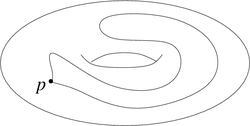
\includegraphics[scale=0.6]{lazo.png}
    \caption{Observamos un lazo de base $p$ contenido en un toro.}
    \label{fig:lazo}
\end{figure}
\end{defi}
\vspace{-5mm}
\begin{defi}
Sea $\ell$ un lazo, definamos el conjunto cociente con la homotopía $\ell \; \sim \; \ell'$:
$$\mathlarger{\mathlarger{\nicefrac{\{ \text{Lazos de base } p \}}{ \sim }}}\; = \; \mathlarger{\pi}_1(X,p)=\text{ grupo fundamental de }  X \text{ en }p$$
Por tanto, un elemento de $\mathlarger{\pi}_1(X,p)$ es una clase $[\ell]$ donde $\ell:[0,1]\longrightarrow X$ es un lazo en $p$.
\end{defi}
\begin{prop}
El grupo fundamental tiene estructura de grupo.
\begin{enumerate}
    \item \underline{El producto está bien definido}
    \begin{dem}
    Se define el producto como $[\ell_1] \cdot [\ell_2] := [\ell_1 \cdot \ell_2]$. Veamos que está bien definido. Sean $\ell_1 \; \sim \; \ell_1'$ y $\ell_2 \; \sim \ell_2' \; \Rightarrow \; \ell_1' \cdot \ell_2' \; \Rightarrow \; \ell_1' \cdot \ell'_2 \; \sim \; \ell_1 \cdot \ell_2 \; \Rightarrow \; [\ell_1' \cdot \ell_2']=[\ell_1 \cdot \ell_2]$. 
    \end{dem}
    \item \underline{Asociatividad}: $(\ell \cdot \ell') \cdot \ell'' \; \sim \; \ell \cdot (\ell' \cdot \ell'')$\\ 
    $([\ell] \cdot [\ell']) \cdot [\ell''] = [\ell] \cdot ([\ell'] \cdot [\ell''])$\\
    Se demuestra de forma similar a la asociatividad en caminos, expuesto en \\ \textbf{\textcolor{blue}{\hyperref[sec:9]{10. Homotopía}}}.
    \item \underline{Existencia de elemento neutro}: $[c_p]$ es el elemento neutro.\\ 
    Por lo visto para cminos, $\ell \cdot c_p \; \sim \; \ell \; \sim \; c_p \cdot \ell$. Por tanto,    $[\ell] \cdot [c_p]=[\ell]=[c_p] \cdot [\ell]$. 
    \item \underline{Existencia del elemento inverso}: $[\ell^-]$ es el elemento inverso de $[\ell]$. \\
    Por lo visto para caminos, $\ell \cdot \ell^{-} \; \sim \; c_p$. Por tanto, $[\ell] \cdot [\ell^-] = [\ell \cdot \ell^-]=[c_p]$. 
\end{enumerate}
\end{prop}
\begin{tcolorbox}
\begin{teo} 
Sea $X$ conexo por caminos, entonces
$$\mathlarger{\pi}_1(X,p) \simeq \mathlarger{\pi}_1(X,q)$$
donde $\simeq$ es un isomorfismo de grupos.
\end{teo}
\end{tcolorbox}

\begin{dem}
Por hipótesis, existe un camino que une $p$ y $q$ tal que $\gamma_{p \cdot q}: [0,1] \longrightarrow X$ con $\gamma_{p \cdot q}(0)=p$ y $\gamma_{p \cdot q}(1)=q$. Definimos el lazo $\ell$ en base $p=\gamma_{p \cdot q}$. Para probar el isomorfismo, probaremos el morfismo en ambos sentidos. En primer lugar:
$$\begin{array}{rrcl}
     \varphi : & \mathlarger{\pi}_1(X,p) & \longrightarrow & \mathlarger{\pi}_1(X,q) \\
     \; & [\ell] & \longmapsto & \varphi(\ell) = [\gamma_{p q}^- \cdot \: \ell \: \cdot \: \gamma_{p q}] \stackrel{\ell \sim \ell'}{=} [\gamma_{p q}^- \cdot \: \ell' \: \cdot \: \gamma_{p q}]  
\end{array}$$
Lo primero que debemos comprobar es si está bien definido, es decir, no depende de los representantes cogidos. Sea $\ell \; \sim \; \ell'$, si $\varphi$ es un morfismo de grupo, debemos comprobar que:
$$\varphi([\ell_1] \cdot [\ell_2])=\varphi([\ell_1]) \cdot \varphi([\ell_2])$$
Donde ya teníamos por definición:
$$\varphi([\ell_1 \cdot \ell_2])=[\gamma_{p q}^- \cdot \: \ell' \: \cdot \: \gamma_{p q}]$$
$$\left. \begin{array}{l}
     \varphi ([\ell_1])=[\gamma_{p q}^- \cdot \: \ell_1 \: \cdot \: \gamma_{p q}]  \\
     \varphi ([\ell_2])=[\gamma_{p q}^- \cdot \: \ell_2 \: \cdot \: \gamma_{p q}] 
\end{array} \right\} \; = \varphi([\ell_1]) \cdot \varphi([\ell_2])=[\gamma_{p q}^- \cdot \: \ell_1 \: \cdot \: \gamma_{p q}] \cdot [\gamma_{p q}^- \cdot \: \ell_2 \: \cdot \: \gamma_{p q}]=$$
$$=[\gamma_{p q}^- \cdot \: \ell' \: \cdot \: \gamma_{p q} \cdot \gamma_{p q}^- \; \cdot  \ell_2 \cdot \; \gamma_{p q}]\stackrel{(1)}{=}[\gamma_{p q}^- \cdot \: \ell_1 \: \cdot \: \ell_2 \: \cdot \: \gamma_{p q}]$$
Donde usamos que $\gamma_{pq} \: \cdot \: \gamma_{pq}^- \; \sim \; c_p \; ^{(1)}$. Por tanto, queda demostrado el morfismo en un sentido. Veamos en el otro sentido:
$$\begin{array}{rrcl}
     \varphi : & \mathlarger{\pi}_1(X,q) & \longrightarrow & \mathlarger{\pi}_1(X,p) \\
     \; & [\ell] & \longmapsto & [\gamma_{p q}^- \cdot \: \ell \: \cdot \: \gamma_{p q}]  \\
     \; & [\gamma_{p q}^- \cdot \: \ell \: \cdot \: \gamma_{p q}] & \longleftarrow & [\ell]
\end{array}$$
La demostración de que el isomorfismo está bien definido en este sentido se demuestra de manera similar al anterior. De esta forma, queda demostrado el isomorfismo de grupos. 
\end{dem}
\section{Aplicaciones}
Sea $f:X \longrightarrow Y$ una aplicación continua y $\ell: I \longrightarrow X$ un lazo en $p$. 
\begin{defi}
Podemos definir la composición de una aplicación con un lazo como sigue:
$$ f \circ \ell : I \stackrel{\ell}{\longrightarrow} X \stackrel{f}{\longrightarrow} Y$$
Donde $f \circ \ell$ es un lazo de $Y$ en $f(p)$.
\end{defi}
\begin{defi}
Si $\ell \; \sim \; \ell'$, entonces $f \circ \ell \; \sim \; f \circ \ell'$. Por lo tanto, existe una homotopía \\ $H: I \times X \longrightarrow X$ continua tal que $H_0 = \ell$ y $H_1 = \ell'$. Podemos definir entonces la composición:
$$f \circ H: I \times X \stackrel{H}{\longrightarrow} X \stackrel{f}{\longrightarrow} Y$$
Tal que:
$$(f \circ H)_0 = f \circ \ell$$
$$(f \circ H)_1 = f \circ \ell'$$
\end{defi}
\begin{cor}
Podemos definir la aplicación $f_*$ de la siguiente forma:
$$\begin{array}{rrcl}
     f_*:  & \bigpi _1(X, p) & \longrightarrow & \bigpi_1(Y, f(p)) \\
     \; & [\ell] & \longmapsto & f_*([\ell])=[f \circ \ell]
\end{array}$$
\end{cor}
\begin{dem}
Debemos probar que está bien definido, es decir que $f_*$ es un morfismo de grupos:
$$f_*([\ell_1] \cdot [\ell_2]) = f_*([\ell_1]) \cdot f_*([\ell_2])$$
Donde tenemos que $f_*([\ell_1] \cdot [\ell_2]) = f_*([\ell_1 \cdot \ell_2]) = [f \circ \ell_1 \cdot \ell_2]$. Análogamente \\ $f_*([\ell_1]) \cdot f_*([\ell_2])= [f \circ \ell_1] \cdot [f \circ \ell_2]=[(f \circ \ell_1) \cdot (f \circ \ell_2)]$. Uniendo ambas igualdades, obtenemos $[f \circ \ell_1 \cdot \ell_2] = [(f \circ \ell_1) \cdot (f \circ \ell_2)]$. Para comprobar rigurosamente, se deben aplicar a un $t$, y se demuestra. \hfill $\square$
\end{dem}
Sean $X \underset{g}{\overset{f}{\rightrightarrows}} Y$ dos aplicaciones y $p \in X$ y $q \in Y$ tales que $f(p)=g(p)=q$
\begin{defi} 
Diremos que $f$ y $g$ son homótopas $f \; \sim \; g$ si existe $H : X \times I \longrightarrow Y$ continua que cumple:
\begin{enumerate}
    \item Para cada $t$, $H_t: X \longrightarrow Y$ cumple que $H_t(p)=q$
    \item La homotopía transforma $f$ en $g$ tal que $H_0=f$ y $H_1=g$
\end{enumerate}
\end{defi}

\begin{defi}
Sean $(X,p)$ y $(Y,q)$ espacios topológicos. Se dice que son homótopos u homotópicamente equivalentes, denotado $(X,p) \; \sim \; (Y,q)$, si existen dos aplicaciones continuas $f : X \longrightarrow Y$ y $g : Y \longrightarrow X$ que cumplen:
\vspace{-4mm}
\begin{itemize}
    \item $f(p) = q; \quad g(q) = p$
    \item $g \circ f \;\sim\; Id_X; \quad f \circ g \;\sim\; Id_Y$
\end{itemize}
\vspace{-4mm}
Estas funciones se denominan equivalencias homotópicas, y se dice que $g$ es la inversa homotópica a $f$.
\end{defi}

\begin{obs}
Es fácil comprobar que todo homeomorfismo es una equivalencia homotópica (siendo su inverso el inverso homotópico). El recíproco no es cierto.
\end{obs}

\section{Morfismo inducido}
\begin{prop}
Dos aplicaciones homótopas inducen el mismo morfismo sobre el grupo fundamental. Es decir, si $f \sim g$, entonces $f_* = g _*$
\end{prop}
\begin{dem}
Sean $f,g : (X,p) \longrightarrow (Y,q)$ aplicaciones homótopas. Los morfismos inducidos son:
$$\begin{array}{rrcl}
     f_*:  & \bigpi _1(X, p) & \longrightarrow & \bigpi_1(Y, q) \\
     \; & [\ell] & \longmapsto & f_*([\ell])=[f \circ \ell]
\end{array}$$
$$\begin{array}{rrcl}
     g_*:  & \bigpi _1(X, p) & \longrightarrow & \bigpi_1(Y, q) \\
     \; & [\ell] & \longmapsto & g_*([\ell])=[g \circ \ell]
\end{array}$$
Si $f \sim g$, existe una homotopía $H:I\times X \rightarrow Y$ tal que $H_0 = f$ y $H_1 = g$. Por tanto, podemos definir otra homotopía $H': I\times X \rightarrow Y$ que, para todo $t \in I$, cumpla $H_t' = H_t \circ \ell$. Ya que $H_0' = f \circ \ell$ y $H_1' = g \circ \ell$, tenemos que $[f \circ \ell] = [g \circ \ell]$, y por tanto $f_*$ y $g_*$ son el mismo morfismo.
\end{dem}

\begin{prop}
Sea $p \in X$ y $f: X \rightarrow Y$, $g : Y \rightarrow Z$ aplicaciones. Entonces, $g_* \circ f_* = (g \circ f)_*$.
\end{prop}
\begin{dem}
Las aplicaciones inducidas por $f$ y $g$ son:
$$\bigpi_1(X,p) \overset{f_*}{\longrightarrow} \bigpi_1(Y,f(p)) \overset{g_*}{\longrightarrow} \bigpi_1(Z,g(f(p)))$$
Sea $[\ell] \in \pi_1(X,p)$. Entonces, $g_* (f_* ([\ell])) = g_* ([f \circ \ell]) = [g \circ (f \circ \ell)] = [(g \circ f) \circ \ell] = (g \circ f)_* ([\ell])$, quedando demostrado.
\end{dem}

\begin{teo} \;
\begin{tcolorbox}
\begin{center}
    
Si $(X,p) \; \sim \; (Y,q)$, entonces $\bigpi_1(X,p) \simeq \bigpi_1(Y,q)$.
\end{center}
\end{tcolorbox}
\end{teo}
\begin{dem}
Sea $f:(X,p) \rightarrow (Y,q)$ una equivalencia homotópica y $g$ su inversa homotópica. Entonces, $g_* \circ f_* = (g \circ f)_* = {Id_X}_*$. Igualmente, $f_* \circ g_* = (f \circ g)_* = {Id_Y}_*$. Ya que ${Id_X}_*$ es la identidad de $\pi_1(X,p)$ y ${Id_Y}_*$ es la identidad de $\pi_1(Y,q)$, tenemos que $g_*$ es la inversa de $f_*$ y, por tanto, esta última es un isomorfismo entre los grupos fundamentales.
\end{dem}
\begin{prop}
    Si $(X,x_o) \sim *$, entonces su grupo fundamental es el trivial: 
    $\mathlarger{\pi}_1(X,x_o)=0$
\end{prop}
\begin{eje}
    ($\mathbb{R}^2-\{0\},q) \sim (S^1,p)$ y sus grupos fundamentales son:$$\mathlarger{\pi}_1(\mathbb{R}^2-\{0\}, q)\simeq \mathlarger{\pi}_1(S^1,p) \simeq \mathbb{Z}$$
    Consideremos en $S^1$ el lazo 
    $$\begin{array}{rrcl}
         \ell : & [0,1] & \longrightarrow & S^1  \\
         & t & \longmapsto & \ell(t)=e^{2 \pi i t} 
    \end{array}$$
    homótopo a $\ell^n$ ($n \in \mathbb{Z}$) y $\ell^n \sim \ell^m \iff n = m$.

        Que el grupo fundamental sea $\mathbb{Z}$ por tanto, significa que este es infinito, abeliano y cíclico, y cuyo generador es el lazo previamente definido.
    \end{eje}
    \begin{eje}
        $\mathlarger{\pi}_1(S^n)=0$
    \end{eje}
\begin{prop}
        Si $X$ es conexo por caminos, $\bigpi_1(X,p) \simeq \bigpi_1(X,q)$
\end{prop}
\begin{dem}
    Para cualesquiera $p,q$ podemos encontrar $\gamma$ de $p$ a $q$, de forma que escribimos el isomorfismo como 
    $$\begin{array}{rcl}
         \bigpi_1(X,p) & \longrightarrow & \bigpi_1(X,q) \\
          \: [\ell ] & \longrightarrow & [\gamma \cdot \ell \cdot \gamma^- ] & 
    \end{array}$$
\end{dem}
\section{Espacio Proyectivo.}
\begin{defi}
    El espacio proyectivo de dimensión $n$: $\mathbb{P}^n$.

    Consideremos $\mathbb{R}^{n+1}-\{0\}$, donde definimos la siguiente relación de equivalencia:
    $$e \sim e' \iff e = \lambda e' (\lambda \neq 0)$$
    \end{defi}
    \begin{defi}
        Llamaremos recta proyectiva a $\mathbb{P}^1$, cuyos puntos son rectas.
    \end{defi}
    De manera que $\mathlarger{\nicefrac{\mathbb{R}^{n+1}-\{0\}}{\sim}} = \mathbb{P}^n$ de forma que $\mathbb{P}^n$ tiene la topología final de la proyección canónica: $\pi: \mathbb{R}^{n+1}-\{0\}\longrightarrow \mathbb{P}^n = \nicefrac{\mathbb{R}^{n+1}}{\sim}$

      Se tiene la proyección canónica:
      $$\begin{array}{rrcl}
           \pi: & \mathbb{R}^{n+1}-\{0\} & \longrightarrow & \mathbb{P}^n = \nicefrac{\mathbb{R}^{n+1}}{\sim}  \\
           & (x_o, x_1, \ldots, x_n) & \longmapsto & \pi(x_o, x_1, \ldots, x_n) = (x_o: x_1: \ldots: x_n)=(\lambda x_o: \lambda x_1: \ldots: \lambda x_n)
      \end{array}$$
      Consideremos el conjunto que tiene la primera coordenada distinta de 0, $U_o=\{((x_o: x_1: \ldots: x_n) \in \mathbb{P}^n \: | \: x_o \neq 0\} \subset \mathbb{P}^n$, de la misma forma se define $U_i$. Se tiene pues que $$\underset{i=0}{\overset{n}{\bigcup}} \: U_i = \mathbb{P}^n$$
      \begin{lem}
          Los $U_i$ son abiertos.
      \end{lem}
      \begin{dem}
         Veamos que $U_o$ es abierto, dado que es antiimagen de un abierto:
         $$\pi^{-1}(U_o)=\{(x_o, x_1, \ldots, x_n) \in \mathbb{R}^{n+1} \: | \: x_o \neq 0\}$$
         el cual s un abierto de $\mathbb{R}^{n+1}$
      \end{dem}
      \begin{lem}
         $U_i$ es homeomorfo a $\mathbb{R}^n$ 
      \end{lem}
      \begin{dem}
          Veamos que $U_o \simeq \mathbb{R}^n$. Denotaremos $\tilde{U_o}=\pi^{-1}(U_o)$. Consideremos la aplicación
          $$\begin{array}{rrcll}
              \mathbb{R}^n & \longrightarrow & \tilde{U_o} & \overset{\pi}{\longrightarrow} & U_o \\
               (x_1, \ldots, x_n) & \longmapsto & (1, x_1, \ldots, x_n) & \longmapsto & (1: x_1: \ldots: x_n) \\
               \big(\frac{x_1}{x_o}, \ldots, \frac{x_n}{x_o}\big) & \longleftarrow & \longleftarrow & \longleftarrow & (x_o: x_1: \ldots: x_n)
          \end{array}$$
          \textcolor{red}{HACER DIAGRAMA GUAPO con la $\psi$}
          
          Queda probar que $\psi: U_o \longrightarrow \mathbb{R}^n$, por tanto para que $\psi$ sea continua basta que $\psi \circ \pi$ lo sea. El único sitio donde podría no haber continuidad sería el conjunto donde $x_o$ se anulara, ya que $\psi \circ \pi(x_o, \ldots, x_n)=(\frac{x_1}{x_o}, \ldots, \frac{x_n}{x_o})$ pero $x_o$ no se anula en $U_o$, luego la composición es continua.     
          \end{dem}

Consideremos la aplicación 
$\pi: \mathbb{R}^{n+1} \supset S^n \longrightarrow \mathbb{P}^n$ que es continua, epiyectiva y la antiimagen de un punto son dos, uno y su antípoda. 

De esta forma, podemos identificar cada punto de la esfera con su antípoda. De esta forma, el conjunto cociente $\nicefrac{S^n}{\sim}=\mathbb{P}^n$ 

Consideremos el espacio proyectivo y veamos que para $n \geq 2$, $\mathlarger{\pi}_1(\mathbb{P}^n)\simeq \nicefrac{\mathbb{Z}}{2 \mathbb{Z}}=\{0,1\}$. Es decir, $c_p \nsim \ell $ pero $c_p \sim \ell^2$.
Esto se debe a que el espacio proyectivo es una cociente de una relación de equivalencia de un espacio con grupo fundamental trivial ($\pi_1(S^n)=0$) dada por clases donde solo hay dos elementos. Esto nos dice que $\ell \sim \ell^-$. 
\section{Homotopía y productos}
Sean $X,Y$ espacios topológicos y $x_o,y_o$ puntos de ellos, respectivamente, y el espacio $X \times Y$
\begin{prop}
    $\pi_1(X \times Y, (x_o,y_o)) \simeq \pi_1(X,x_o) \times \pi_1(Y,y_o)$
\end{prop}
\begin{dem}
    Consideremos las proyecciones $\pi_X:X \times Y \longrightarrow X$ y $\pi_Y$, que inducen morfismo en los grupos fundamentales $\pi_{X_*}: \pi_1(X\times Y)\longrightarrow\pi_1(X)$ y $\pi_{Y_*}$. De forma que se induce un morfismo en el producto de ellos dado por 
    $$\begin{array}{rrcl}
         \phi:& \pi_1(X\times Y) & \longrightarrow & \pi_1(X) \times \pi_1(Y)\\
         & [ l ] & \longmapsto & (\pi_{X_*}([ \ell ]), \pi_{Y_*}([\ell])) 
    \end{array}$$
    Veamos ahora el morfismo inverso:
    $$\begin{array}{rrcl}
         \psi: & \pi_1(X) \times \pi_1(Y)  & \longrightarrow & \pi_1(X\times Y)  \\
         & ([ l ], [\gamma]) & \longmapsto & [\ell \times \gamma]
    \end{array}$$
    De forma que los lazos son de la forma $\ell: I \longrightarrow X$ y $\gamma: I \longrightarrow Y$, luego $\ell \times \gamma: I \ \longrightarrow X \times Y$. 

    Veamos pues que este morfismo está bien definido. Si $\ell \sim \ell'$, veamos si $\ell \times \gamma \sim \ell' \times \gamma$. \textcolor{red}{TERMINAR}
\end{dem}
\begin{ejer}
    Si $(X,x_o) \sim (X',x_o)$ y $(Y,y_o) \sim (Y',y_o)$, entonces $(X \times Y, (x_o,y_o)) \sim (X' \times Y', (x_o,y_o))$
\end{ejer}
\begin{cor}
    De esta forma, podemos hallar el grupo fundamental de espacios dados por productos directos, por ejemplo: \vspace{-5mm}
    \begin{itemize}
        \item El cilindo:

        $\pi_1(S^1 \times \mathbb{R})=\pi_1(S^1) \times \pi_1(p) =\pi_1(S^1)=\mathbb{Z}$
        \item El toro:

        Dado que $\mathbb{T}=S^1 \times S^1$, $\pi_1(\mathbb{T})=\pi_1(S^1)\times \pi_1(S^1)=\mathbb{Z} \times \mathbb{Z}$
    \end{itemize}
\end{cor}
\begin{obs}
    El teorema de Van Kampen, asegura que si $X=U \cup V$ con $U,V$ y $U \cap V$ conexos por caminos, si $\pi_1(U)=\pi_1(V)=0$, entonces $\pi_1(X)=0$.
\end{obs}
\begin{cor}
    Veamos el grupo fundamental de $S^1$. Consideremos la aplicación:
    $$\begin{array}{rrcl}
         \mathbb{R} & \longrightarrow & S^1 = \mathlarger{\nicefrac{\mathbb{R}}{\mathbb{Z}}} \\
         t & \longmapsto & e^{2 \pi i t} 
    \end{array}$$
    Esta aplicación se denomina revestimiento, de forma que $\mathbb{R}$ es un revestimiento de $S^1$ \textcolor{red}{METER FOTO HELICOIDE} y la antiimagen de un punto es $\mathbb{Z}$    
\end{cor}
\section{\textcolor{blue}{Espacios simplemente conexos}}
Sea $X$ un espacio topológico

\begin{defix}
$X$ es \textbf{simplemente conexo} cuando es conexo por caminos y su grupo fundamental es el grupo trivial.
\begin{obsx}
Que el grupo fundamental de $X$ sea el grupo trivial es equivalente a decir todo lazo se puede deformar a un punto. De la misma forma, diremos $X$ no tiene ``agujeros".

En términos formales, todo lazo $\ell: [0,1] \longrightarrow X$ de base $p$ es contractible de forma continua mediante una homotopía $H: I \times I \longrightarrow X$ tal que $H(t,0)=\ell(t)$ y $H(t,1)=p$.
\end{obsx} 
\end{defix}
\begin{obsx}
En un espacio simplemente conexo se cumple que entre todo par de puntos existe una única clase de homotopía de caminos, es decir, todos los caminos que los conectan son homotópos entre sí. El término "simplemente conexo" viene precisamente de esta propiedad: sólo existe una forma, salvo homotopía, de conectar con un camino cualquier par de puntos del espacio.

Por ejemplo, un toro no es simplemente conexo, y entre un par de puntos podemos escoger dos caminos no homótopos, uno por cada ``lado".
\end{obsx}
\begin{ejex}
     La esfera $S^2$ es simplemente conexa, como se puede observar en la figura, todo lazo se puede contraer a un punto (y es trivialmente conexa por caminos).
    \begin{figure}[h]
    \centering
    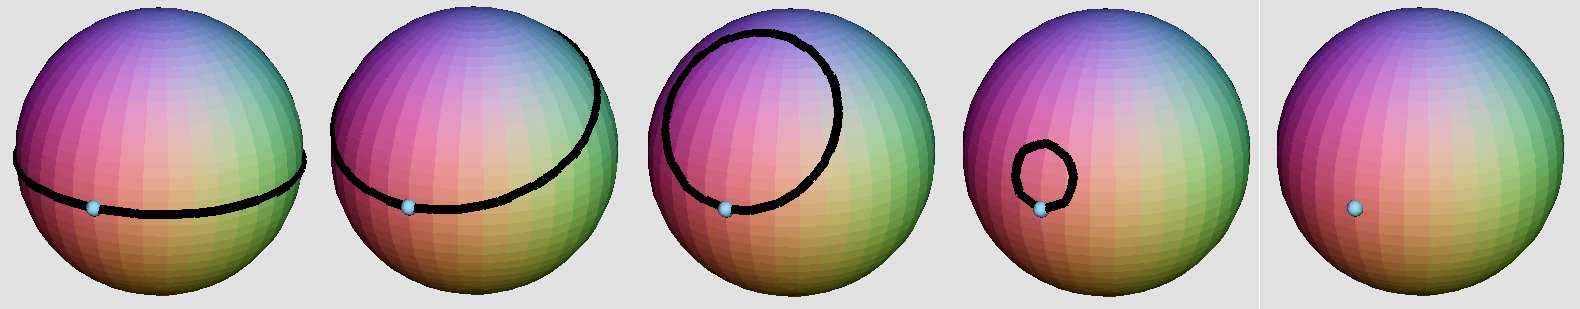
\includegraphics[scale=0.27]{esfera.jpeg}
    \caption{Esfera con un lazo que se contrae}
    \label{fig:esfera}
\end{figure}
\end{ejex}
\chapter{\textcolor{blue}{DIMENSIÓN DE ESPACIOS TOPOLÓGICOS}}
\chapter{FIBRADOS}

\begin{defix}  
Un \textbf{fibrado} consiste en una cuaterna $ (E,B,f ,F)$ donde $E, \: B$ y $F$ son espacios topológicos y $f: E \longrightarrow B$ es una aplicación continua y epiyectiva, de manera que para cualquier $x \in B$ existe un entorno $U \in B$ de $x$ y un homeomorfismo \\ $\phi : f^{-1}(U) \longrightarrow U \times F$ tal que  $f =\pi \circ \phi$  con $\pi : U\times F\longrightarrow U$, $\pi(x,y)=x$. 
\end{defix}
\begin{corx}
Equivalentemente, podemos decir que para todo punto de $B$ existe un entorno $U$ y un homeomorfismo $\phi$  tal que el siguiente diagrama conmuta: 
$$\mathlarger{\xymatrix{
E \; \supseteq \; f^{-1}(U) \ar[r]^{\quad \phi} \ar[d]_{f} & U \times F \ar[ld]^{\pi} \\
B \; \supseteq \; U \quad \; \; \; \;& 
}} $$
La aplicación $f$  es abierta por ser una proyección en un producto cartesiano y $B$ tiene la topología cociente. El espacio $B$ se llama el espacio de base del fibrado, $E$ el espacio total, para cualquier $x \in B$, $f^{-1}(x)$ se llama la fibra en $x$ y la función $\pi$ se llama la proyección. Se denota $E \: |_{U}= f^{-1}(U)$ y se dice que $f$ es localmente trivial y el par ($U,\phi$) es una trivialización local. Es habitual escribir $E$ en vez de ($E,B,f ,F$) si $f$ y $F$ se pueden entender por contexto. Tambi{\'e}n se suele decir que $E$ es un fibrado sobre $B$.
\end{corx}
\begin{defi} El producto fibrado o fibrado trivial es un ejemplo de fibrado y viene dado por $(B \times F, B, \pi, F)$ con $\pi : U \times F \longrightarrow U $
\end{defi}
\begin{ejex}
Veamos algunos ejemplos interesantes de fibrados:
\begin{itemize}
    \item \textit{Cilindro $\mc{C}$} 
    
    Sea $[-1,1] \subset \mathbb{R}$ un segmento (\textit{fibra}) y $\mathbb{S}^1$ la \textit{base}, podemos definir un fibrado:
        $$\xymatrix{
            [-1,1] \; \; \ar@{^{(}->}[r] & \; \mc{C} \ar[d] \\
            & \mathbb{S}^1 
        } $$
        donde $\mc{C}$ es el cilindro de altura $h=2$, que llamamos \textit{espacio total}.
    
    \item \textit{Banda de Möbius} $\mathbb{M}$
    
    Utilizando la misma \textit{fibra} y la misma $base$ podemos conseguir otros resultados. Es el caso de la banda de Möbius $\mathbb{M}$:\\
    
        \vspace{-0.6cm}
        \begin{figure}[h]
        \raggedleft
        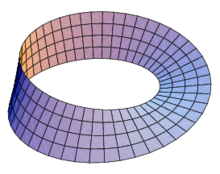
\includegraphics[scale=0.5]{moebius.png}
        \end{figure}
        \vspace{-3.4cm} \hspace{2cm} $\xymatrix{
            [-1,1] \; \; \ar@{^{(}->}[r] & \; \mathbb{M} \ar[d] \\
            & \mathbb{S}^1 
        } $ 
        \; \\
        \: \\
        \; \\
        Ahora la base tambi{\'e}n es $\mathbb{S}^1$ (en la mitad de la banda, se observa una circunferencia) y la fibra es el segmento previamente elegido, pero ahora se va rotando para construir el resultado obtenido.
        \item \textit{Toro} $\mathbb{T}$
        \item \textit{Botella de Klein} $\mathbb{K}$
\end{itemize} 
\end{ejex}

\chapter{VARIEDADES TOPOLÓGICAS}
%% ♪ ♫ ♪ ♫ ♪ ♫ ♪ ♫ ♪ ♫ ♪ ♫ ♪ ♫ ♪ ♫ ♪ ♫ ♪ ♫ ♪ ♫ ♪ ♫ ♪ ♫ ♪ ♫ ♪ ♫ ♪ ♫ ♪ ♫ ♪ ♫ %%




\appendix
\setcounter{chapter}{0}
\chapter{SEMINARIOS 2021-2022} \label{P1}
\section{Seminario 1}
\hspace{-6mm}Sea $(X,\mc{T}_d)$ un espacio topológico, con $\mc{T}_d$ la topología asociada a una distancia $d$ en $X$. 
Diremos que un subconjunto $\mathcal{U}$ de $X$ es abierto si es vacío o cumple que: $$\forall \; x \in \mathcal{U} \; \; \exists \; r_x > 0 \;\; / \;\; B(x,r_x) \subseteq \; \mathcal{U}$$

\begin{ejer}
Probar que es una topología.
\end{ejer}

\begin{prop}
Toda bola es un abierto.
\end{prop}
\begin{dem}
Sea $\mc{B}(x,r)$, $y \in \mc{B}(x,r)$. Probaremos que existe $r_y > 0$ tal que $\mc{B}(y,r_y) \subseteq \mc{B}(x,r)$\\
Tenemos que $y \in \mc{B}(x,r) \; \Leftrightarrow \; d(x,y) < r  \; \Rightarrow \; r - d(x,y) > 0$\\
Tomemos $r_y = r - d(x,y)$. Veamos que $\mc{B}(y,r_y) \subseteq \mc{B}(x,r)$\\
Sea $z \in \mc{B}(y,r_y) \; \Rightarrow \; d(y,z) < r_y$. A su vez, $d(x,z) < d(x,y) + d(y,z) < d(x,y) + r_y < d(x,y) + (r - d(x,y)) \; \Rightarrow \; d(x,z) < r \; \Rightarrow \;  z \in \mc{B}(x,r) \; \Rightarrow \; \mc{B}(y,r_y) \subseteq \mc{B}(x,r)$
\end{dem}

\begin{prop}
Un subconjunto $\mc{U}$ de $X$ es abierto $\Leftrightarrow \; \mc{U}$ es una unión de bolas.
\end{prop}
\begin{dem}\; \\ \vspace{-12mm}
\begin{itemize}
    \item $\Rightarrow$ 
    $\mc{U}$ es unión de bolas (abiertos), por lo que es un abierto.
    \item $\Leftarrow$ 
    $\mc{U}$ es abierto para cada $x \in \mc{U}$, por lo que existe $r_x > 0$ tal que $\mc{B}(x,r_x) \subseteq \mc{U}$. Entonces, $\mc{U} = \underset{x \in \mathcal{U}}{\bigcup} \mc{B}(x,r_x) $
\end{itemize}
\end{dem}

\begin{obs}
Las bolas (\textcolor{blue}{abiertas}) forman una base de la topología.
\end{obs}
\vspace{5mm}
\begin{prop}
$X$ es separado.
\end{prop}
\begin{dem}
Sean $x,y$ dos puntos distintos de $X$. Sea $r = d(x,y) > 0$.\\
Tenemos que $x \in \mc{B}(x,\nicefrac{r}{2}),\; y \in \mc{B}(y,\nicefrac{r}{2})$. Calculemos la intersección de estas bolas suponiendo un $z \in \mc{B}(x,\nicefrac{r}{2}) \cap \mc{B}(y,\nicefrac{r}{2})\; \Rightarrow \; d(z,x) < \nicefrac{r}{2}, \;\; d(z,y) < \nicefrac{r}{2}$.\\
$r = d(x,y) \leq d(x,z) + d(y,z) < \nicefrac{r}{2} + \nicefrac{r}{2} < r$. Esto es una contradicción, por lo que \\$\mc{B}(x,\nicefrac{r}{2}) \cap \mc{B}(y,\nicefrac{r}{2}) = \varnothing$ y se concluye.
\end{dem}



\section{Seminario 2}

Sea $\beta$ una base para una topología en $X$.
\begin{prop}
\;
$$\mc{T}_{\beta} = < \beta > = \{ \mathcal{U} \in \underset{B \in \beta}{\bigcup} B \} = \{ \mathcal{U} \in X \;\;\; / \;\;\; \forall \; x \in \mathcal{U} \;\;\; \exists \;\;\; B \in \beta \;\;\; /\;\; \; x \in B \subseteq \mathcal{U}\}$$
es una topología en $X$.
\end{prop}
\begin{dem} \:
\begin{enumerate} 
\item $\varnothing \in \mc{T}_{\beta} \quad , \quad X \in \mc{T}_{\beta}$ (por la definición de base)
\item $\mathcal{U} \; ,\; \mathcal{V} \in \mc{T}_{\beta} \; \Rightarrow \; \mathcal{U} \cap \mathcal{V} \in \mc{T}_{\beta}$ \\
$\mathcal{U} \in \mc{T}_{\beta} \; \Rightarrow \;\;\; \forall \;\; x \in \mathcal{U}  \;\;\; \exists \;\;\; x \in B_x \subseteq \mathcal{U}$ \\
$\mathcal{V} \in \mc{T}_{\beta} \; \Rightarrow \;\;\; \forall \;\; y \in \mathcal{V}  \;\;\; \exists \;\;\; y \in B_y \subseteq \mathcal{V}$ \\
\vspace{3mm}$ \mathcal{U} \cap \mathcal{V} \in \mc{T}_{\beta} \;\;\; , \;\;\; x \in  \mathcal{U} \cap \mathcal{V} \; \Rightarrow \;\;\; \left\{ \begin{array}{l}
      \exists \;\; B_x \in B \; / \; x \in B_x \subseteq \mathcal{U}   \\
      \exists \;\; B_x' \in B \; / \; x \in B_x' \subseteq \mathcal{V} 
\end{array} \right.$\vspace{3mm}

$x \in B_x \cap B_x' \subseteq \mathcal{U} \cap \mathcal{V} \; \Rightarrow \;\;\; x \in \hat{B}_x \subseteq B_x \cap B_x' \subseteq \; \mathcal{U} \cap \mathcal{V}$\\ \vspace{3mm}

$\left. \begin{array}{cc}
     \mathcal{U} = \underset{B_U \in \beta}{\bigcup} B_U  \\
     \mathcal{V} = \underset{B_V \in \beta}{\bigcup} B_V 
\end{array} \right\} \quad \mathcal{U} \cap \mathcal{V} = \underset{B_U, B_V \in \beta}{\bigcup} (B_U \cap B_V) = \underset{\hat{B} \in \beta}{\bigcup} \hat{B}$
\vspace{3mm}
\item $\{ \mathcal{U}_i \}_{i \in I} \; \subseteq \; \mc{T}_{\beta} \; \Rightarrow \;\;\; \bigcup \; \mathcal{U}_i \in \mc{T}_{\beta}$ \\
$\underset{i \in I}{\bigcup} \; \mathcal{U}_i = \underset{i \in I}{\bigcup}(\underset{B_{U_i} \in \beta}{\bigcup} B_{U_i} ) = \underset{B \in \beta}{\bigcup} B \; \in \mc{T}_{\beta}$ \\
\end{enumerate}
\end{dem}

\begin{defi}
Sea $(X,\mc{T})$ un espacio topológico.\\
$\beta \in \mathcal{P}(X)$ es una base para una topología $\mc{T}_{\beta}$ de $X$.

Decimos que $\beta$ es una base de la topología $\mc{T}_x$ si  $\mc{T}_x = \mc{T}_{\beta}$ si se cumple:
\begin{enumerate}
    \item $\beta \in \mc{T}_x$ (los $B\in \beta$ son abiertos en $(X, \mc{T}_x)$)
    \item $\mathcal{U} \in \mc{T}_x \; \Longleftrightarrow \;\forall x \in \mathcal{U} \;\; \exists \;\; B_x \in \beta$ tal que $x \in B_x \subseteq \mathcal{U}$
\end{enumerate}
\end{defi}
\newpage
\begin{prop}
Una familia $\beta \in \mathcal{P}(X)$ es una base de $(X, \mc{T}_x)$ si y solo si se cumplen las condiciones 1 y 2. 
\end{prop}

\begin{defi}
$S \subseteq \mathcal{P}(X)$ es una sub-base para una topolgía si $X = \underset{B_i \in S}{\bigcup}\; B_i$\
Toda base de una topología es una sub-base, pero el recíproco no es cierto.

Llamamos base $B_S$ asociada a una sub-base $S$ a aquella cuyos elementos son intersecciones finitas de elementos de $S$.
$$B_S = \{ S_{i_1} \; \cap \;\;\dots \;\; \cap S_{i_r} \}\text{    con }S_{i_j} \in S$$
\end{defi}

\begin{prop}
Existencia de bases en espacios topológicos.\\ \vspace{3mm}
Todo espacio topológico $(X,\mc{T}_X)$ tiene como base la propia topología $\mc{T}_X$.
\end{prop}

\begin{eje}
     Base para la topología discreta. $$\beta = \{ \; \{x\} \;\; \forall x \in X\}$$ 
    Es base: \vspace{-4mm} \begin{itemize}
        \item $\{x\}$ son abiertos de $(X,\mc{T}_X)$
        \item $\forall \;\; \mathcal{U} \in \mc{T}_X$   ,  $\mathcal{U} = \underset{x \in \mathcal{U}}{\bigcup}\;  \{x\}$
    \end{itemize}
    Además, esta es la menor base de $(X,\mc{T}_X)$, es decir, si $\beta'$ es otra base de $(X,\mc{T}_X)$, entonces $\beta \in \beta'$
    \begin{dem}
    $x \in X \; \Rightarrow \;\; \{x\}$ es abierto.\\
    $\beta'$ es base de $\mc{T}_X$.\\
    $\exists \;\; B' \in \beta' \;\; / \;\; x \in B' \; \subseteq \; \{x\}  \; \Rightarrow \;\; B' \in \{x\}$
    \end{dem}
\end{eje}

\pagestyle{plain}
\section{Seminario 3} \label{P3}
En este capítulo se demuestran los ejercicios propuestos la sección \textbf{\textcolor{blue}{\hyperref[sec:adherencia]{1.4. Adherencia}}}. Recordemos las nociones básicas de dicha sección.

Sea $(X, \mc{T})$ un espacio topológico, $A$ un subconjunto $: \; A \neq \emptyset$
\begin{defi} Cierre de $A$

$\overline{A}=\{ \text{puntos adherentes a }A \}=\{ x \in X \; / \; \; \mc{U}_x \cap A \neq \emptyset \; \forall \; \mc{U}_x \in \mc{T}_x \text{ con } x \in \mc{U}_x\}$
\end{defi}
\begin{propi} \; \\
\vspace{-10mm}\begin{enumerate}
    \item $A \subseteq \overline{A}$ (Por definición ya que  si $x \in A$, $U_x \cap A=\{ x \}$ al menos)
    \item $\overline{A}$ es cerrado en $X$
    \begin{proof}
    $\overline{A} \text{ es cerrado } \Leftrightarrow \; X-\overline{A}$ abierto, es decir, para cada $x \in X-\overline{A}$ existe un abierto $\mc{U} \; : \; x \in \mc{U} \subseteq X-\overline{A}$ 
    
    Por reducción al absurdo, supongamos que $x \nin \overline{A}$, $x \in X-\overline{A}$ luego $\exists \; \mc{U} \in \mc{T}_x$ tal que $x \in \mc{U}$ y $\mc{U} \cap A = \emptyset \; \; \; (\mc{U} \subseteq X-A)$ 
    
    Supongamos que existe $y \in \mc{U} \cap \overline{A}$, entonces $y \in \mc{U}, \; y \in \overline{A}$ $\Rightarrow \mc{U} \cap A \neq \emptyset$ (ya que todos los abiertos que contienen a $y$ cortan con $A$) $\longrightarrow \;$ \underline{Contradicción}
    
    $\Rightarrow \mc{U} \cap A = \emptyset \Rightarrow x \in \mc{U} \subseteq X - \overline{A} $, abierto por ser $\underset{x \in X-\overline{A}}{\bigcup} \; \mc{U}_x$
    \end{proof}
    
    \item $\overline{A}$ es el menor cerrado que contiene a $A$, es decir, si $C \subseteq X$ es un cerrado y $A \subseteq C$, entonces $\overline{A} \subseteq C$.
    \begin{proof}
    Por reducción al absurdo, supongamos que existe $x \in \overline{A}$ tal que $x\not\in C$, con lo que $x\in X-C$, que es abierto. Tenemos entonces que:
    $$(X-C) \cap A = \varnothing$$
    ya que $A\subseteq C$. Llegamos a una contradicción, ya que todos los abiertos que contienen a $x$ deben tener intersección no nula con $A$ por la definición de punto adherente.
    \end{proof}
    \begin{obs}
    Se verifica que $\overline{A} = \underset{A \subseteq C}{\bigcap} C$, ya que el menor conjunto que contiene a otro es la intersección de todos los conjuntos que lo contienen.
    \end{obs}
    
    \item $A = \overline{A} \; \Leftrightarrow$ $A$ es cerrado
    \begin{proof}
    Si $A = \overline{A}$, $A$ es cerrado porque $\overline{A}$ lo es. En el otro sentido, si $A$ es cerrado, el menor cerrado en el que está contenido ($\overline{A}$) es él mismo.
    \end{proof}
    \end{enumerate}
\end{propi}



\chapter{SEMINARIOS 2022-2023} \label{S2}
\section{Seminario 1. G1.}
\justifying
\begin{enumerate}
    \item \justifying Demuestra que $\mc{T}=\{\emptyset,\mathbb{N}\} \cup \{A \subset \mathbb{N}\: | \: A \text{ contenga tan s{\'o}lo n{\'u}meros pares}\}$ determina una topolog{\'i}a (por abiertos) de $\mathbb{N}$. Determina si los siguientes subconjuntos son abiertos, cerrados, las dos cosas o ninguna de las dos:
    $$A_1=\{90, 2^{10}, 5^{21}-1\}, \qquad A_2=\{\text{n{\'u}meros primos}\}\quad \text{y} \quad A_3 = \{\text{n{\'u}meros impares}\}.$$
    \begin{sol}
    Veamos en primer lugar que es una topolog{\'i}a, para lo cual debe cumplir las condiciones para ello. En efecto:
    \begin{itemize}
        \item $\emptyset, \: \mathbb{N} \in \mc{T}$ por definici{\'o}n. 
        \item Sean $U, V \in \mc{T}$, entonces
        $$x \in U \cap V \Rightarrow \left.\begin{array}{cc}
             x \in U \Rightarrow & x \text{ es par} \\
             x \in V \Rightarrow & x \text{ es par}
        \end{array}\right\} \Rightarrow U \cap V \in \mc{T}$$
        \item Sea $\{U_i\}_{i \in I} \in \mc{T}$ una familia arbitraria de abiertos, entonces
        $$x \in \underset{i \in I}{\bigcup}\: U_i \Rightarrow x \in U_j \: (\text{para alg{\'u}n } j \in I) \Rightarrow x \text{ es par.}$$
        
        Por lo tanto, $\underset{i \in I}{\displaystyle\bigcup}\: U_i \in \mc{T}$.
    \end{itemize}
    Concluyendo as{\'i} que efectivamente se trata de una topolog{\'i}a. 
    
    Veamos ahora la naturaleza topol{\'o}gica de los conjuntos propuestos:
    \begin{itemize}
        \item $A_1=\{90, 2^{10}, 5^{21}-1\}$ es abierto ya que est{\'a} compuesto por n{\'u}meros pares; claramente 90 es divisible por 2, $2^{10}$ tambi{\'e}n, y $5^{21}-1$ sabiendo que toda potencia de 5 acaba en 5, restando 1 acaba en 4, por tanto divisible por 2. No es cerrado ya que su complematario contiene impares, por tanto no abierto.
        \item $A_2=\{\text{n{\'u}meros primos}\}$ no es abierto ya que (a excepi{\'o}n del 2) ning{\'u}n n{\'u}mero primo es par. Tampoco es cerrado ya que su complementario contendr{\'i}a n{\'u}meros pares e impares que no sean primos, luego no ser{\'a} abierto.
        \item $A_3 = \{\text{n{\'u}meros impares}\}$ es cerrado ya que su complementario son todos los pares, luego abierto. No es abierto ya que no contiene ning{\'u}n par. 
    \end{itemize}
    \end{sol}
    \item \justifying En $\mathbb{Z}_{+}$ consideramos la familia de subconjuntos $U \subseteq \mathbb{Z}_{+}$ que satisfacen la siguiente propiedad: si $n \in U$ entonces, cada divisor de $n$ tambi{\'e}n pertenece a $U$. Probar que dicha familia de subconjuntos es una topolog{\'i}a en $\mathbb{Z}_{+}$, que no es la discreta.
    \begin{sol}
    Veamos en primer lugar que efectivamente es una topolog{\'i}a:
    \begin{itemize}
        \item $\mathbb{Z}_+ \in \mc{T}$ ya que cualquier $n \in \mathbb{Z}_+$, sus divisores tamb{\'e}n est{\'a}n en $\mathbb{Z}_+$. El vac{\'i}o deber{\'i}a añadirse artificialmente.
        \item Sean $U, V \in \mc{T}$, entonces
        $$n \in U \cap V \Rightarrow \left.\begin{array}{cc}
             n \in U \Rightarrow & \text{divisores de } n \in U \\
             n \in V \Rightarrow & \text{divisores de } n \in V
        \end{array}\right\} \Rightarrow \text{divisores de } n \in U \cap V \Rightarrow U \cap V \in \mc{T}$$
        \item Sea $\{U_i\}_{i \in I} \in \mc{T}$ una familia arbitraria de abiertos, entonces
        $$n \in \underset{i \in I}{\bigcup}\: U_i \Rightarrow n \in U_j \: (\text{para alg{\'u}n } j \in I) \Rightarrow \text{divisores de } n \in U_j$$
        
        Por lo tanto, $\underset{i \in I}{\displaystyle\bigcup}\: U_i \in \mc{T}$.
    \end{itemize}
    Concluyendo as{\'i} que efectivamente se trata de una topolog{\'i}a. 
    
    Veamos ahora que no se trata de la topolog{\'i}a discreta. Consideremos un $n \in \mathbb{Z}_+$ no primo, entonces $n$ es abierto de $\mathbb{Z}_+$ con la topolog{\'i}a discreta, en cambio no lo es con la definida previamente, ya que no contiene a sus divisores. Por tanto concluimos que $\mc{T}_{dis} \neq \mc{T}$.
    \end{sol}
    \item  Sean $\mc{T}_1$ y $\mc{T}_2$ dos topolog{\'i}as en $X$. Probar que $\mc{T}_1$ es m{\'a}s fina que $\mc{T}_2$ si y s{\'o}lo si todo cerrado de $\mc{T}_2$ es cerrado de $\mc{T}_1$.
    \begin{sol}
    \begin{itemize}
        \item $\Rightarrow)$ Supongamos que $\mc{T}_2 \subset \mc{T}_1$. Dado un cerrado de $\mc{T}_2$, su complementario ser{\'a} abierto de $\mc{T}_2$, que por ser $\mc{T}_1$ m{\'a}s fina, lo ser{\'a} de ella tambi{\'e}n. Luego $C$ tambi{\'e}n ser{\'a} cerrado de $\mc{T}_1$.
        \item $\Leftarrow)$ Dado un abierto $U \in \mc{T}_2$, su complementario ser{\'a} cerrado de $\mc{T}_2$ y por hip{\'o}tesis, cerrado de $\mc{T}_1$. Como $U^c$ es un cerrado de $\mc{T}_1$, $U$ es abierto de $\mc{T}_1$, por tanto $\mc{T}_2 \subset \mc{T}_1$.
    \end{itemize}
    \end{sol}
    \item Sea $(X, \mc{T})$ un espacio topol{\'o}gico. Entonces $\mc{T}$ es la topolog{\'i}a discreta si y s{\'o}lo si para cada $x \in X$ el subconjunto que define $\{x\}$ es abierto.
    \begin{sol}
    \begin{itemize}
        \item $\Rightarrow)$ Si $X$ tiene la topolog{\'i}a discreta, todo subconjunto $U \subseteq X$ es abierto. En particular, podemos considerar los subconjuntos formados por un solo punto (para $x\in X$, el conjunto $\{x\}$), los cuales ser{\'a}n abiertos.
        \item $\Leftarrow)$ Dado un subconjunto $U \subseteq X$, podemos expresarlo como uni{\'o}n de sus puntos, de forma que $$\displaystyle U = \underset{\underset{x_i \in U}{i}}{\bigcup} \{x_i\}$$
        Como cada uno de los $\{x_i\}$ es abierto, $U$ tambi{\'e}n lo ser{\'a}. Por tanto, la topolog{\'i}a es la discreta, ya que todo subconjunto es abierto. 
    \end{itemize}
    \end{sol}
    \item Probar que la intersecci{\'o}n infinita de abiertos de $\mathbb{R}$ (con la topolog{\'i}a usual) no es, en general, un abierto.
    \begin{sol}
    Veamos para ello un contraejemplo. Consideremos la sucesi{\'o}n de abiertos de $\mathbb{R}$ definida por $U_n = \{B(0,\nicefrac{1}{n})\}_{n \in \mathbb{N}}=\{(-\nicefrac{1}{n},\nicefrac{1}{n})\}_{n \in \mathbb{N}}$. Se tiene que 
    $$\underset{n \in \mathbb{N}}{\bigcap} U_n = \{0\}$$
    Luego $\underset{n \in \mathbb{N}}{\bigcap} U_n$ no es un abierto en $\mathbb{R}$ con la topolog{\'i}a usual.  
    \end{sol}
\end{enumerate}
\section{Seminario 2. G1.}
\begin{enumerate}
    \item \justifying Sea $\mc{T}_{cf}$ la topología cofinita sobre el conjunto $X$, e $Y \subset X$. Demuestra que la topología inducida $(\mc{T}_{cf})_Y$ es la topología cofinita de $Y$, ($Y, \mc{T}_{cf})$
    \begin{sol}
    Por un lado, $\mc{T}_{cf}=\{U \subset X \: | \: X - U \text{ es finito}\}$, y se pide demostrar que $(\mc{T}_{cf})_Y=\{S \subset Y \: | \: Y-S \text{ es finito}\}$ es igual a $\mc{T}_{cf_{|Y}}=\{S \subset Y \: | \: S = U \cap Y \: | \: U \in \mc{T}_{cf}\}$.
    
    Veamos en primer lugar que \textcolor{orange}{$\mc{T}_{cf_{|Y}}\subseteq (\mc{T}_{cf})_Y$}. Dado que trabajamos con la topología cofinita, será mejor que consideremos cerrados en vez de abiertos. 
    
    Sea $C$ un cerrado en $\mc{T}_{cf}$, entonces $C$ es finito. Sea $C$ un cerrado en $\mc{T}_{cf_{|Y}}$, entonces $C=C' \cap Y$ con $C'$ cerrado en $\mc{T}_{cf}$, entonces $C'$ es finito. Veamos que $C' \cap Y$ es cerrado en $(\mc{T}_{cf})_Y$. Sabiendo que $C'\cap Y \subset C'$ por tanto finito y en $(\mc{T}_{cf})_Y$. 
    
     Veamos ahora que \textcolor{orange}{$(\mc{T}_{cf})_Y \subseteq \mc{T}_{cf_{|Y}}$}. Sea $C$ un cerrado en $(\mc{T}_{cf})_Y$ con $C \subseteq Y$, entonces $C$ es finito. Busquemos un $C' \subseteq X$ finito tal que $C=C'\cap Y$. En efecto ese $C'$ que buscamos es $C$, ya que $C=C \cap Y$, luego $C \in \mc{T}_{cf_{|Y}}$. 
    \end{sol}
    \item Sea $(X, \mc{T})$ un espacio topológico y $A \subseteq X$. Llamamos interior de $A$, y lo denotamos por $A^{\circ}$ al mayor abierto de $X$ contenido en $A$. Probar que 
\begin{enumerate}[a)]
    \item $A^{\circ}=\{ \text{puntos interiores a } A\}$, donde $x \in X$ se dice que es un punto interior a $A$ si $A$ es un entorno suyo.
    \begin{sol}\: 
    
    \underline{$A
    ^{\circ} \subseteq \{\text{puntos interiores}\}$}
    
    Si $x \in A^{\circ}$, entonces $\exists
    \: U \subseteq A$ tal que $x \in U$. Dado que $A^{\circ}$ es el mayor abierto contenido en $A$, tomamos $U=A^{\circ}$, y por tanto $x$ es un punto interior.
    
    \underline{$\{\text{puntos interiores}\} \subseteq A
    ^{\circ}$}
    
    Si $x$ es un punto interior, existe un entorno suyo $U \subseteq A$, por tanto $x \in  A^{\circ}$.
    \end{sol}
    \item $A^{\circ}=A$ si y sólo si $A$ es abierto.
    \begin{sol}
    $\Rightarrow$) Supongamos que $A^{\circ}=A$. Esto implica que $A$ es un entorno de todos sus puntos, luego es abierto.
    
    $\Leftarrow)$ Si $A$ es abierto, es un entorno de cada uno de sus puntos, luego $A=A
    ^{\circ}$
    \end{sol}
    \item $(A^{\circ})^{\circ}=A^{\circ}$.
\begin{sol}
Como $A^{\circ}$ es abierto, su interior será él mismo, luego $(A^{\circ})^{\circ}=A^{\circ}$
\end{sol}
\end{enumerate}
\item Calcula en $(\mathbb{R}, \mc{T}_{inf})$ el interior y el cierre de los siguientes subconjuntos:
$$[1,2) \quad (- \infty, 0) \quad (-\infty, 0] \quad (1,+\infty) \quad (0,3] \quad \left\{\frac{1}{q} \: | \: \:  q \in \mathbb{Z}, \: q \neq 0 \right\}$$
\begin{sol}
Tenemos que $\mc{T}_{inf}=\{U \subset \mathbb{R} \: | \: \forall a \in U \: \exists \: b > a : [a,b) \subseteq U\}$ de forma que una base es $\beta = \{[a,b) \subseteq \mathbb{R}\}$. Entonces, podemos expresar un abierto como $\displaystyle U=\underset{a,b \: \in \mathbb{R}}{\bigcup} [a,b)$, luego un cerrado es de la forma $\displaystyle C=\bigcap [a,b)^c=\bigcup ((-\infty,a) \cup [b,\infty))$
\begin{itemize}
    \item $(-\infty,0)^{\circ}=(-\infty,0)$ ya que es abierto.
    
    $\overline{(-\infty,0)}=(-\infty,0)$ por ser cerrado, ya que $(-\infty,0)^c=[0,\infty)$ es abierto.
    \item $(-\infty,0]^{\circ}=(-\infty,0)$
    
     $\overline{(-\infty,0]}=(-\infty,0]$ ya que es cerrado (su complementario es abierto $(0,\infty)$)
     
     \item $\left\{\frac{1}{q} \: | \: \:  q \in \mathbb{Z}, \: q \neq 0 \right\}^{\circ}= \emptyset$ ya que $\nexists [0,b)$ ya que $0$ no pertenece al conjunto. 
     
     $\overline{\left\{\frac{1}{q} \: | \: \:  q \in \mathbb{Z}, \: q \neq 0 \right\}}=\{\nicefrac{1}{q}\} \cup \{0\}$
\end{itemize}
\end{sol}
\item Sea $(X, \mc{T})$ un espacio topológico tal que si $x \neq y$ existe un entorno de $x$ que no contiene a $y$, o bien un entorno de $y$ que no contiene a $x$. Si en $X$ la intersección arbitraria de abiertos es un abierto, probar:
\begin{enumerate}[a)]
    \item La relación $x \leq y$ si $x \in \overline{\{y\}}$ es una relación de orden en $X$.
    \begin{sol}
    \begin{enumerate}[a)]
    \item \underline{Reflexividad:}  $x \leq x$ $\forall x$ 
    
    Dado que $x \in \overline{\{x\}}$, se verifica
        \item \underline{Antisimétrica:} si $x \leq y$ e $y \leq x$, entonces $x=y$.
        
        Trivialmente, $x \in \overline{\{x\}}$ e $y \in \overline{\{y\}}$. Por otro lado, dadas las desigualdades, $x \in \overline{\{y\}}$ e $y \in \overline{\{x\}}$. Entonces $\overline{\{x\}}=\overline{\{y\}}$, luego $x=y$ por ser $T_0$
        \item \underline{Transitividad:} si $x \leq y$ e $y \leq z$, entonces $x \leq z$.
        
        Tenemos que $x \in \overline{\{y\}}$ y que $y \in \overline{\{z\}}$. Esto implica que todo $U \ni x$ cumple que $y \in U$ y que todo $V \ni y$ cumple que $z \in V$. Por tatno, cualquier abierto $W \ni x$ cumple que $z \in W$. Por tanto, $x \in \overline{\{z\}}$.
    \end{enumerate}
    \end{sol}
    \item Si denotamos $U_x=\{y \in X \: | \: x \leq y\}$, probar que $U_x$ es el menor abierto contiene a $x$ y que $\beta=\{U_x \: | \: x \in X\}$ es una base de la topología de $X$. De hecho, es la mínima, esto es, si $\mc{B}$ es otra base para $X$, entonces $\beta \subseteq \mc{B}$.
    \begin{sol}
    Consideremos $U_x=\{y \in X \: | \: x \leq y\}$ es el menor abierto 
    \end{sol}
\end{enumerate}
\end{enumerate}
\section{Seminario 3. G1.}
\begin{enumerate}
    \item Demuestra las siguients propiedades:
\begin{enumerate}[a)]
    \item Si $A_1 \subset A_2$, entonces $\overline{A}_1 \subset \overline{A}_2$. 
    \begin{sol}
    Sea $x \in \overline{A}_1$, entonces $\forall \: U_x \ni x$, $U_x \cap A_1 \neq \emptyset$. Como $A_1 \subseteq A_2$, \\ $U_x \cap A_2 \neq \emptyset \: \Rightarrow \: x \in \overline{A}_2$.
    \end{sol}
    \item $\overline{A \cap B}= \overline{A} \cup \overline{B} $
    \begin{sol}
    Veamos que $\overline{A \cup B} \subseteq \overline{A} \cup \overline{B}$. Sea $x \in \overline{A \cup B}$, entonces $\forall \: U_x \ni x$, $U_x \cap (A \cup B) \neq \emptyset$. Por tanto, $(U_x \cap A) \cup (U_x \cap B) \neq \emptyset$. Es decir, o bien $U_x \cap A \neq \emptyset$ o bien $U_x \cap B \neq \emptyset$, por lo que o bien $U_x \subseteq \overline{A}$ o bien $U_x \subseteq \overline{B}$. Entonces $U_x \subseteq \overline{A} \cup \overline{B}$.
    
    Por otro lado, $A \subseteq A \cup B$ y $B \subseteq A \cup B$, por el apartado  a) $\overline{A} \subseteq \overline{A \cup B}$ (igual para $\overline{B}$). Por tanto, $\overline{A} \cup \overline{B} \subseteq \overline{A \cup B}$. 
    \end{sol}
    \item $\overline{A \cap B} \subset \overline{A} \cap \overline{B}$. Encuentra un ejemplo en el que no no se cumpla la igualdad.
    \begin{sol}
    Dado que $A \cap B \subseteq A$ y $A \cap B \subseteq B$, por el apartado a), $\overline{A \cap B} \subseteq \overline{A}$ y $\overline{A \cap B} \subseteq \overline{B}$, por lo que al estar en ambos, en específico está en la intersección, luego $\overline{A \cap B} \subset \overline{A} \cap \overline{B}$. 
    
    Un ejemplo en el que no se cumple la igualdad es tomando $A=(0,1)$ y $B=(1,2)$. $\overline{A}=[0,1]$ y $\overline{B}=[1,2]$. Entonces $\overline{A \cap B}=\overline{(0,1) \cap (1,2)}=\emptyset$ pero $\overline{A} \cap \overline{B}=[0,1]\cap [1,2]=1$.
    \end{sol}
    \item En el caso no finito, $\bigcup_j \overline{A_j} \subseteq \overline{\bigcup A_j}$. Encuentra un ejemplo en el que no se dé la igualdad. 
    \begin{sol}
    Claramente, $A_j \subseteq \bigcup A_j$ para cualquier $j$, luego $\overline{A_j} \subseteq \overline{\bigcup A_j}$ por el apartado a). Luego si están incluidos cada uno de ellos, también lo está su unión, por lo que  $\bigcup_j \overline{A_j} \subseteq \overline{\bigcup A_j}$.
    
    Para ver un ejemplo en el que no se cumple la igualdad, consideremos la familia de subconjuntos $A_j=\{q_i \in \mathbb{Q}\}$. Tenemos por un lado que $\bigcup A_j = \bigcup \{q_i\}=\mathbb{Q}$, luego $\overline{\bigcup A_j} = \overline{\mathbb{Q}}= \mathbb{R}$. Por otro lado, para cada $j$, $\overline{A_j}=\{q_i\}$ (por ser cada punto ``aislado"), luego $\bigcup \overline{A_j}=\{q_i\}=\mathbb{Q}$. Queda así por tanto terminado el ejemplo de la no igualdad. 
    \end{sol}
\end{enumerate}
\item En un espacio topológico $(X,\mc{T})$, dado un subconjunto $A \subset X$ se cumple: \textcolor{red}{TERMINAR}
\begin{enumerate}[a)]
    \item $\partial(A) \cap A^{\circ} = \emptyset$
    \begin{sol}
        Sea $x \in \partial(A)=\overline{A} \cap \overline{(X-A)}$, entonces para todo entorno abierto $U_x$ de $x$ se cumple que: 
        $$U_x \cap A \neq \emptyset \qquad \text{ y } \qquad U_x \cap (X-A)\neq \emptyset$$
        Por tanto, como $U_x$ corta a $A$ y a su complementario, $U_x \nsubseteq A$, es decir, $x \nin A^{\circ}$ (ya que un entorno suyo no está contenido en $A$).
    \end{sol}
    \item $A$ es abierto $\iff \: \partial (A) \cap A = \emptyset$ 
    \begin{sol}
        $\Rightarrow)$ Por ser $A$ abierto, $A=A^{\circ}$, luego por el apartado $a)$, $$\emptyset=\partial (A) \cap A^{\circ} =  \partial (A) \cap A $$
        $\Leftarrow)$ Supongamos que $\partial (A) \cap A = \emptyset$, entonces para todo $x \in A$ (de forma que $x \nin \partial(A)$) todo entorno suyo $U $, cumple que $U \cap A \neq \emptyset$, pero por no ser frontera, $U \cap (X-A) = \emptyset$, luego $x \in U \subseteq A$, luego $A$ es entorno de todos sus puntos, luego abierto. 
    \end{sol}
    \item $A$ es cerrado $\iff \: \partial(A) \subset A$
    \item $A$ es abierto y cerrado $\iff \: \partial(A)=\emptyset$ 
\end{enumerate}
\item Demuestra que todo subconjunto finito $A$ de $\mathbb{R}$ con la topología usual es cerrado. Prueba además que $\partial(A)=A$.
\begin{sol}
Dado que $A$ es finito, lo podemos expresar como unión (disjunta) de sus elementos, luego $A=\{a_1\} \cup \cdots \cup \{a_n\} \: \forall a_i \in \mathbb{R}$ y $n \in \mathbb{N}$. Como con la topología usual cada punto es cerrado, $A$ es unión finita de cerrados, luego es cerrado. 

Veamos ahora que $\partial(A)=A$. En especial, $\partial(\{a\})=\{a\}$ ya que $\{a\}=B(c,r)\cap\{a\}$ y $B(c,r) \cap (X-\{a\}) \neq \emptyset$, luego todo abierto corta a $\{a\}$ y a $X-\{a\}$, por tanto $\{a\}$ es un punto frontera. Ahora dado que 
$$A = \bigcup_{i=1}^n\{a_i\} \: \Rightarrow \: \partial(A)=\partial\left(\bigcup_{i=1}^n\{a_i\}\right)=\bigcup_{i=1}^n \partial(\{a_i\})=\bigcup_{i=1}^n\{a_i\}=A$$
\end{sol}
\item Sea $(X, \mc{T})$ un espacio topológico, y $A \subset X$. Prueba que $A^{\circ} \neq \emptyset$ si y sólo si tiene intersección con todo conjunto denso $D \subset X$.
\begin{sol} \justifying
$\Leftarrow$) Por una de las definiciones dadas de subconjuntos densos, este corta a todo abierto, luego $A \cap D \neq \emptyset \: \forall \: D$, luego $A \neq \emptyset$ y por tanto, por la definición de interior, $A^{\circ} \neq \emptyset$. 

$\Rightarrow$) Supongamos ahora que $A^{\circ}= \emptyset$. Sea $U$ un abierto cualquiera, entonces $U \cap (X-A)=\emptyset$, por lo que $U \subseteq A$. Al ser $A^{\circ}$ el máximo abierto que contiene a $A$, $A^{\circ}\neq \emptyset$, llegando a una contradicción.  

Por otro lado, suponiendo también que $A^{\circ}= \emptyset$, para un abierto $U$ cualquiera, $U \cap (X-A) \neq \emptyset$ (por ser $A= \emptyset$), luego $X-A$ es denso, pero por hipótesis $A \cap (X-A)=\emptyset$, llegando así a otra contradicción. 
\end{sol}
\item Sea $Y$ un espacio topológico $T_2$ y $f: X \longrightarrow Y$ y $g: X \longrightarrow Y$ dos aplicaciones. Probar que:
\begin{enumerate}[a)]
    \item El conjunto de puntos $C=\{x \in X \: | \: f(x)=g(x)\}$ es un cerrado de $X$.
    \begin{sol}
    Veamos que $X-C$ es abierto. Sea $x \in X-C$, entonces $f(x) \neq g(x)$. Por ser $Y$ separado ($T_2$), existen entornos $U_{f(x)}, \: V_{g(x)}$ disjuntos ($U_{f(x)} \cap V_{g(x)} = \emptyset$). 
    
    Por otro lado, $f^{-1}(U)$ es abierto y $g^{-1}(V)$ es abierto en $X$ por ser continuas y ser antiimágenes de abiertos. Entonces $f^{-1}(U) \cap g^{-1}(V)$ es abierto (por ser intersección de abiertos) y además $x \in f^{-1}(U) \cap g^{-1}(V)$ (por estar en $X-C$). Entonces, tenemos que $$f^{-1}(U) \cap g^{-1}(V) \cap C = \emptyset$$
    porque $C$ son los $y$ tales que $f(y)=g(y)$ pero $f^{-1}(U) \cap g^{-1}(V)$ son los entornos de los $x$ tales que $f(x) \neq g(x)$, luego son disjuntos. 
    
    Supongamos que existe $z \in f^{-1}(U) \cap g^{-1}(V) \cap C$, en cuyo caso, $f(z) \in U, g(z) \in V$ y $f(z)=g(z)$, lo cual es una contradicción por la hipótesis de que $U \cap V = \emptyset$. Por tanto $X-C$ es abierto. 
    \end{sol}
    \item Si $f$ y $g$ coincide en un subespacio denso de $X$, entonces $f$ y $q$ son iguales.
    \begin{sol}
    Si $f$ y $g$ coinciden en un denso $D$, entonces $D \subseteq C$, luego sus cierres cumplen que $\bar{D} \subseteq \bar{C}$, y al ser $D$ denso, $\bar{D}=X$, luego $X=C$, es decir, coinciden en todo el espacio, y por tanto, son la misma.     \end{sol}
    \item Sea $f : \mathbb{R} \longrightarrow \mathbb{R}$ continua de modo que $f(q)=0$ para todo $q \in \mathbb{Q}$. Demuestra que $f(x)=0$ para todo $x \in \mathbb{R}$.
    \begin{sol}
    Es directo por el apartado anterior. $\mathbb{Q}$ es denso en $\mathbb{R}$, y la aplicación $f=0$ en ellos, por tanto lo es en todo el espacio.
    \end{sol}
\end{enumerate}
\end{enumerate}


%% ♪ ♫ ♪ ♫ ♪ ♫ ♪ ♫ ♪ ♫ ♪ ♫ ♪ ♫ ♪ ♫ ♪ ♫ ♪ ♫ ♪ ♫ ♪ ♫ ♪ ♫ ♪ ♫ ♪ ♫ ♪ ♫ ♪ ♫ ♪ ♫ %%

\chapter{EJERCICIOS 2022-2023}
\section{Espacios Topológicos}
\begin{ejer} \textbf{30.} Sean $\mc{B}_1$ y $\mc{B}_2$ dos bases de abiertos de $X$, que generan las topologías $\mc{T}_1$ y $\mc{T}_2$ respectivamente. Demuestra que $\mc{T}_1$ es más fina que $\mc{T}_2$ si y solo si para cada $x \in X$ y para cada ${B}_2 \in \mc{B}_2$ tal que $x \in \mc{B}_2$ existe un básico $B_1\in \mc{B}_1$ tal que $x \in B_1 \subset B_2$.
\end{ejer}

\section{Elementos de un espacio topológico}
\begin{ejer}
    \textbf{45. } \textit{Puntos aislados}. Dado $A \subset X$, se dice que $x \in A$ es un punto aislado de $A$ si $\{x\}$ es un abierto de $A$ con la topología inducida en $A$ como subconjunto de $X$. Se denota por $A^a$ el conjunto de puntos aislados de $A$. Prueba las siguientes igualdades:
    \begin{enumerate}[a)]
        \item $A' \cap A^a = \emptyset$, siendo $A'$ el conjunto de puntos de acumulación de $A$.
        \begin{sol}
            Sea $x \in A^a$, existe $U$ abierto en $X$ tal que $\{x\}=U \cap A$, entonces \\ $(U-\{x\})\cap A = \emptyset$ que es lo contrario a la definición de puntos de acumulación, luego $x \nin A'$. 
        \end{sol}
        \item $\overline{A}=A' \cup A^a$ 
\begin{sol} Veamos que se cumplen ambas inclusiones:
    
        $\boxed{\supseteq}$ Por un lado, $A^a \subseteq A \subseteq \overline{A}$ (porque los puntos aislados son puntos del propio subconjunto) y por otro lado, $A' \subseteq \overline{A}$ (ya que sus entornos reducidos cortan a todo abierto), por tanto, $\overline{A} \supseteq A' \cup A^a$.

        $\boxed{\subseteq}$ Sea $x \in \overline{A}-A'$. Como $x \in \overline{A}$, entonces $\forall \: U, \: U \cap A \neq \emptyset$. Por otro lado, $x \nin A'$, entonces existe $V \ni x$ abierto en $X$ tal que $(V-\{x\})\cap A = \emptyset$. Por tanto, la única opción para $V \cap A=\{x\}$, entonces $x \in A^a$.       
\end{sol}
        \item $(\overline{A})^a \subset A^a$, y deduce que si $A$ no tiene puntos aislados, su cierre tampoco.
        \begin{sol}
            Sea $x \in (\overline{A})^a$, entonces existe $U$ abierto tal que $$\{x\}=U \cap \overline{A}$$
            En particular, $x \in A$, luego $V \cap A \neq \emptyset$ para todo abierto $V\ni x$. Entonces, \\ $\emptyset \neq U \cap A \subseteq U \cap \overline{A} = \{x\}$, luego $U \cap A = \{x\}$, es decir, $x \in A^a$.
        \end{sol}
    \end{enumerate}
\end{ejer}
\begin{ejer}
    \textbf{46. } Sea $(X,\mc{T})$ un espacio topológico, y considera en $Y \subset X$ la topología inducida de $X$, $(Y, \mc{T}_{|_Y})$. Dado $A \subset Y$, probar que:
    \begin{enumerate}
        \item $A^{\circ} \cap Y \subseteq A^{\circ}_Y=\{$interior de $A$ en $(Y, \mc{T}_{|_Y})\}$.
        \item $\overline{A} \cap Y=\overline{A}_Y=\{$cierre de $A$ en $(Y, \mc{T}_{|_Y})\}$.
        \item $\partial_Y(A) \subseteq \partial(A)\cap Y$.
    \end{enumerate}
\end{ejer}
\begin{ejer}
    \textbf{63. } Sea $(X,\mc{T})$ un espacio $T_1$, y sea un subconjunto $Y$ de $X$. Demostrar que la intersección de todos los abiertos que contienen a $Y$ es el propio $Y$. Probar que $x \in X$ es cerrado.
\end{ejer}
\begin{sol}
    
\end{sol}
\begin{ejer}
    \textbf{64.} Demuestra que la topología del punto incluído es $T_0$ pero no $T_1$.
\end{ejer}
\begin{sol}
    La topología del punto incluido es $\mc{T}_a=\{U \subseteq X \: / \: a \in U\}\cup \{\emptyset\}$. 
    
    Veamos en primer lugar que no es $T_1$. Un espacio es $T_1$ si para cada $x,x'$ exisen $U_x, U_{x'}$ tales que $x' \nin U_x$ y $x \nin U_{x'}$. En el caso de $\mc{T}_a$, todos los abiertos contienen al punto $a$, luego no existen abiertos que no contengan a $a$.

    Por otro lado, veamos que es $T_0$. Consideremos $x \neq y$ pero con $\bar{x}=\bar{y}$, entonces 
    $$\left\{\begin{array}{l}
         x \in \overline{\{y\}} \:  \Rightarrow \: \forall U \ni x, \: y \in U \: ^{(1)} \\
         y \in \overline{\{x\}} \Rightarrow \: \forall V \ni y, \: x \in V 
    \end{array}  \right.$$
    Continuando en $(1)$, 
    si $y=a$, entonces $a \in \overline{\{x\}}$. Por otro lado, si $y \neq a$, entonces $X-\{y\}$ es abierto (por contener a $a$) y $x \in X-\{y\}$, pero $y \nin X-\{y\}$, llegando a una contradicción, \textcolor{red}{por suponer que $x\neq y$. REVISAR}
    \end{sol}
\begin{ejer}
    \textbf{65.} Sea $X$. un conjunto y considera la topología discreta $\mc{T}_d$ y la topología cofinita $\mc{T}_{cf}$. Determina si $(X, \mc{T}_d)$ y $(X, \mc{T}_{cf})$ cumple los axiomas $T_0$, $T_1$ y $T_2$.
\end{ejer}
\begin{sol}
    
\end{sol}
\section{Continuidad}
\begin{ejer}
    \textbf{78.} Sea $Y$ un espacio topológico $T_2$. Si existe $f:X\longrightarrow Y$ contnua e inyectiva, demuestra que $X$ también es $T_2$.
\end{ejer}
\begin{sol}
    
\end{sol}
\section{Conexos}
\begin{ejer}
\textbf{85.} Probar que $X$ es conexo si y sólo si todo cerrado no trivial tiene frontera no vacía. 
\end{ejer}
\begin{sol}
    En primer lugar y como vimos en el ejercicio 2. del Seminario 3., $A \subseteq X$ es abierto y cerrado $\iff \: \partial (A)=\emptyset$,  por tanto se tiene la siguiente cadena de siysolosis:

    $X$ conexo $\iff$ no existen abiertos-cerrados $\iff$ los únicos cerrados $C$ con $\partial (C)=\emptyset$ son triviales $\iff$ todo cerrado no trivial tiene frontera vacía.
\end{sol}
\begin{ejer}
    \textbf{86.} Probar que la recta de Sorgenfrey $(\mathbb{R}, \mc{T}_{inf})$ no es conexa. ¿Y el espacio de Sierpinski, es decir, $S=\{0,1\}$ con $\mc{T}_S=\{\emptyset, \{1\}, S\}$?
\end{ejer}
\begin{sol}
    Considerando $Y=(-\infty,a)$ con $a \in \mathbb{R}$, $Y$ es abierto en $(\mathbb{R}, \mc{T}_{inf})$ (por serlo en $(\mathbb{R}, \mc{T}_{u})$ y $\mc{T}_{inf} \subseteq \mc{T}_u$, ya que $[x,y) \subset (-\infty,a)$). De la misma forma, $Y$ es cerrado por ser $[a,\infty)$ abierto, luego $Y$ es abierto y cerrado, luego la recta de Sorgenfrey no es conexa. \textcolor{red}{SIERPINSKI}
\end{sol}
\begin{ejer}
    \textbf{87.} Demuestra las siguientes propiedades sobre conjunto de un espacio topológico $X$:
    \begin{enumerate}[a)]
        \item Sea $Y \subseteq X$ un subespacio conexo. Si $X=A \sqcup B$ con $A,B$ abiertos no vacíos, entonces $Y \subseteq A$ ó $Y \subseteq B$.
        \begin{sol}
            
        \end{sol}
        \item Si $A$ conexo y $B \subseteq A$ es tal que $A \subseteq B \subseteq \overline{A}$, entonces $B$ es conexo. En particular, si $A$. es conexo entonces $\overline{A}$ es conexo. 
        \begin{sol}
            
        \end{sol}
        \item Si $A$ y $B$ son conexos y $A \cap B \neq \emptyset \: \Rightarrow \: A \cup B$ es conexo. 
        \item Si $A$ y $B$ son cnexos y $\overline{A} \cap B \neq \emptyset \: \Rightarrow \: A \cup B$ es conexo.
        \item Si $A$ y $B$ son cerrados de $X$ , $A\cup B$ y $A\cap B$ son conexos, entonces $A$ y $B$ son conexos.
        \item Da un ejemplo que demuestre que si $A$ ó $B$ no son cerrados, la propiedad anterior no es cierta.
    \end{enumerate}
\end{ejer}
\begin{ejer}
    \textbf{88.} Sean $\mc{T}$ y $\mc{T}'$ dos topologías en $X$. Si $\mc{T} \subset \mc{T}'$, ¿qué relación existe entre que $(X,\mc{T})$ sea conexo y que lo sea $(X,\mc{T}')$?
\end{ejer}
\begin{ejer}
    \textbf{97.} Los números racionales $\mathbb{Q}$ en $(\mathbb{R}, \mc{T}_u)$ son totalmente desconexos.
\end{ejer}
\begin{ejer}
    \textbf{99. }\begin{enumerate}[a)]
        \item 
        \item
    \end{enumerate}
\end{ejer}
\begin{ejer} \textbf{102.}
    Sea $(X, \mc{T})$ un espacio localmente desconexo (los únicos conexos son los puntos).
    Probar que:
    $$(X,\mc{T}) \text{  es localmente conexo } \iff (X,\mc{T})\text{ es discreto.}$$
\end{ejer}
\begin{ejer}
    \textbf{103.} Sea $X$ infinito y separado $T_2$, entonces es totalmente desconexo.
\end{ejer}
\begin{ejer}
    \textbf{109.} Sea $(X,\mc{T})$ con la topología del punto incluido $\mc{T}=\{U \in X\: / \: p \in U\}\cup \{\emptyset\}$. Estudiar si es conexo por caminos, localmente conexo o conexo. Estudiar lo mismo con la topología del punto excluido.
\end{ejer}
\section{Compactos}
\begin{ejer}
    \textbf{111.} Probar que la compacidad es una condición absoluta.

    Es decir, que dado $Y \subseteq X$ entonces $(Y, \mc{T}_{|_Y})$ es compacto si y solo si $\forall \: \{U_i\}_{i \in I}$ abiertos de $X$ de manera que $Y \subseteq \underset{i \in I}{\bigcup}\: U_i$ existe $\{U_j\}_{j=1}^n \subseteq \{U_i\}_{i \in I}$ tales que $Y \subset \underset{i \in I}{\overset{n}{\bigcup}}\: U_j$
\end{ejer}
\begin{sol}\:\vspace{-5mm}
\begin{itemize}
    \item$\Rightarrow$) Suponemos ($Y,\mc{T}_{|_Y}$) compacto. Sea $Y \subseteq \underset{i \in I}{\bigcup} U_i$ con $U_i$ abiertos de $X$. La familia $\{V_i=U_i \cap Y\}$ son abiertos en $Y$ y $\underset{i \in I}{\bigcup} \: V_i=\underset{i \in I}{\bigcup}(U_i \cap Y)=Y$. 

Como supusimos $(Y, \mc{T}_{|_Y})$ compacto, entonces existe un subrecubrimiento finito, es decir, 
$$Y=\bigcup_{i \in I}^n (\underbrace{U_i \cap Y}_{\subseteq U_i}) \Rightarrow Y \subseteq \bigcup_{i \in I}^n \: U_i$$

\item $\Leftarrow$) Sea $Y=\underset{i\in I}{\bigcup}V_i$ con $V_i$ abiertos en $Y$, es decir, $V_i=U_i\cap Y$ con $U_i$ abiertos en $X$. en particular:
$$Y=\underset{i\in I}{\bigcup}V_i=\underset{i\in I}{\bigcup}(U_i\cap Y)\subseteq \underset{i\in I}{\bigcup}U_i$$
Por hipótessis, $Y$ es compacto con la topología inducida, luego existe una subfamilia finita $\{U_1,\ldots, U_n\}$ de abiertos en $X$ tales que $Y\subseteq\underset{i\in I}{\bigcup}U_i$, por tanto:
$$Y=\bigcup_{i=1}^n (U_i \cap Y)=\bigcup_{i=1}^n V_i$$
luego $Y$ es compacto con la topología inducida.
\end{itemize}
\end{sol}
\begin{ejer}
    \textbf{112.} Sea $(X,\mc{T})$ un espacio topológico y $\{x_n\}_{n \in \mathbb{N}}$ una sucesión en $X$. 
    \\ Si $\displaystyle x \in \lim_{n \to \infty} x_n$ probar que $Y=\{x_n\}_{n \in \mathbb{N}} \cup \{x\}$ es compacto.
\end{ejer}
\begin{sol}
    Véase que 
    $$x \in \lim_{n \to \infty}\,x_n \iff \forall \: U_x \text{ entorno de } x \: \exists \: n_o \in \mathbb{N} : \: \forall n \geq n_o \: \Rightarrow x_n \in U_x$$
Como $\{\{x_n\} \cup \{x\}\}=Y \subset \underset{i}{\bigcup} U_i \: \Rightarrow \exists \: i_o \in I$ tal que $x \in U_{i_o}$. Como $x \in \lim_{n \to \infty}\displaystyle$ existe $n_o \in \mathbb{N}$ tal que $\forall \: n \geq n_o$, $x_n \in U_{i_o}$

Cada $x_k$ con $1\leq k\leq n_0-1$ estará en algún $U_k\in \{U_i\}_{i\in I}$ tales que $x_k\in U_{i_k}$. Por tanto $Y=\{\{x_n\}\cup \{x\}\}\subseteq U_{i_1}\cup\cdots \cup U_{i_{n_0-1}}\cup U_{i_0}$

Veamos qué sucede si el límite no es único. Supongamos que $x,y \in \Lim{n}{\infty}{x_n}$, entonces ahora $Y=\{\{x_n\} \cup \{x\} \cup \{y\}\}$. Es compacto ya que solo basta añadir un abierto más a la colección (subrecubrimiento) que habíamos considerado previamente, luego sigue siendo un subrecubrimiento finito, y por tanto, compacto. \textbf{En cambio}, si tuvieramos un número infinito de límites, $Y$ no sería compacto, ya que necesitaríamos infinitos abiertos para crear el subrecubrimiento, luego no sería finito, y por tanto $Y$ no sería compacto. 
\end{sol}
\begin{ejer} \textbf{113.} 
Sea $X$ un espacio topológico y $\mc{T}'\leq \mc{T}$ dos topologías. Estudiar la compacidad o la no compacidad de $(X,\mc{T}')$ en función de la compacidad o no compacidad de $(X,\mc{T})$
\end{ejer}
\begin{sol}\:\vspace{-5mm}
\begin{itemize}
    \item Supongamos que $(X,\mc{T})$ es compacto. Sea $X=\underset{i\in I}{\bigcup}U_i'$ con $U_i'\in \mc{T}'$. Como $(X,\mc{T}$) es compacto y $\mc{T}'\leq \mc{T}$ se tiene que $\displaystyle X=\bigcup_{i=1}^n U_i'$ (dado que $U_i'\in \mc{T}$).
\item Si $(X, \mc{T})$ no es compacto, entonces $(X, \mc{T}')$ puede ser compacto o no. Veamos un ejemplo de un espacio que no es compacto, pero con una topología más fina sí lo es.  

Todo espacio trivial es compacto, si $X=\underset{i}{\bigcup} \:U_i$ con $U_i \in \mc{T}_{rivial}$, entonces $U_i=\{X\}$ para algún $i$.
\end{itemize}
\begin{eje}
    $(\mathbb{R}, \mc{T}_u) \leq (\mathbb{R}, \mc{T}_{inf})$ donde ninguno es compacto. Si $$\mathbb{R}=\bigcup_{n \in \mathbb{N}} \: (-n,n) \: \cancel{\Rightarrow} \: \mathbb{R}=\bigcup_{i=1}^m (-n,n)$$ 
\textcolor{red}{revisar la flecha}\end{eje}
\end{sol}
\begin{ejer}
Sea $(X,\mc{T})$ un espacio topológico e $Y\subseteq X$ un subconjunto. Probar que si $|Y|<\infty$, entonces $Y$ es compacto, o lo que es lo mismo, probar que todo espacio topológico finito es compacto.
\end{ejer}
\begin{sol}
Sea $(X,\mc{T})$ un espacio topológico finito con $X=\{x_1,\ldots,x_n\}$. Si tenemos que $X=\underset{i\in I}{\bigcup}U_i$, necesariamente cada $x_j\in U_{i_j}$, luego $X=\bigcup_{i=1}^n U_{i_j}$ y con lo cual $X$ es compacto
\end{sol}
\begin{ejer}\textbf{115.}
Sea $(X,\mc{T})$ un espacio topológico discreto. Probar que $X$ es compacto si y solo si es finito. Probar también que $X$ es localmente compacto.
\end{ejer}
\begin{sol}\:\vspace{-5mm}

    \item$\Leftarrow$) finito $\Rightarrow$ compacto (ver ejercicio 113)

\item $\Rightarrow)$ Si $X$ es discreto veamos que $X$ es finito. Como $X$ es discreto, $\{x\}$ es abierto $\forall \: x \in X$ y $X=\underset{x \in X}{\bigcup}\{x\}$.   

Como $X$ es compacto, existen $x_1,\ldots, x_n\in X$ tales que $X=\bigcup_{i=1}^n\{x_n\}$, luego es finito (siendo el conjunto $\{x\}$ un entorno compacto de cada $x\in X$)

\end{sol}
\begin{ejer}
    \textbf{116.} Sea $(X,\mc{T})$ compacto, probar que 
    \begin{enumerate}
        \item Pueden existir subonjuntos infinitos discretos
        \item No existen cerrados infinitos discretos
    \end{enumerate}
\end{ejer}
\begin{sol}
    \begin{enumerate}
        \item Consideremos el intevalo $[0,1]\subseteq\mathbb{R}$ con la topología inducida. Sabemos que es compacto por ser cerrado y acotado. Sea $[0,1]\supseteq Y=\{\frac{1}{n}\}_{n\in\mathbb{N}}$. Dado $\frac{1}{n}=y\in Y$ tenemos que $y=\left(\frac{1}{n}+\varepsilon,\frac{1}{n}-\varepsilon\right)\cap [0,1]\cap Y$, luego $y$ es abierto y por tanto $Y$ es discreto (también es infinito).
        \item Sea $C$ un cerrado $C \subseteq (X, \mc{T})$(compacto), entonces $C$ es compacto. Por el ejercicio 115, entonces no es discreto e infinito. (Si $C$ es discreto, compacto $\Leftrightarrow$ finito).
    \end{enumerate}
\end{sol}
\begin{ejer}
    \textbf{117.} Probar que $(0,1)$ no es compacto pero sí localmente compacto.
\end{ejer}
\begin{sol}
  El intervalo $(0,1)$ no es compacto por ser homeomorfo a $\mathbb{R}$. Podemos también buscar un recubrimiento el que no podemos extraer un subrrecubrimiento finito. Definimos el recubrimiento por abiertos
  $$(0,1)=\bigcup_{n \in \mathbb{N}} \left(\dfrac{1}{n},1\right)$$
  Si $(0,1)$ fuera compacto, existirían $n_1, \ldots, n_r \in \mathbb{N}$ tales que $\displaystyle (0,1)=\bigcup_{i=1}^r \left(\dfrac{1}{n_i},1\right)=\left(\dfrac{1}{\max{\{n_i}\}}, 1\right)$, lo cual es una contradicción.

Veamos ahora que es localmente compacto. Dado $x\in (0,1)$, la colección de bolas cerradas $\{\bar{B}_{\varepsilon}(x)\}_{\varepsilon>0}$ es una base de entornos compactos de $x$.


\end{sol}
\begin{ejer}
    \textbf{118.} $X$ compacto $\iff$ toda familia de cerrados $\{C_i\}_{i \in I}$ de $X$ con la propiedad de las intersecciones finitas ($\underset{i\in I}{\bigcap} C_i \neq \emptyset \: \forall$ colección finita ) satisface que $\displaystyle \bigcap_{i \in I} C_i \neq \emptyset$
\end{ejer}
\begin{sol}\:\vspace{-5mm}
\begin{itemize}
    \item $\Rightarrow)$ Supongamos que $X$ es compacto y que para cualquier colección de cerrados $\{C_i\}_{i\in I}$ se verifica que $\underset{j\in J}{\bigcap}C_j\neq \emptyset$ para cualquier $J\subseteq I$ finito.
    
    Supongamos que $\underset{i\in I}{\bigcap}C_i=\emptyset$, entonces, tomando complementarios se tiene que $X=\underset{i\in I}{\bigcup}C_i^c$, luego los $C_i^c$ son un recubrimiento abierto de $X$. Por ser $X$ compacto existirá un subrecubrimiento finito, lo cual es una contradicción, ya que implicaría que existe $J\subseteq I$ finito tal que $\underset{j\in J}{\bigcap}C_j = \emptyset$
\item $\Leftarrow)$ Sea $X=\bigcup_{i \in I} \displaystyle U_i$ con $U_i$ abiertos, entonces
$$\emptyset=\bigcap_{i \in I} \underbrace{U_i^c}_{cerrado}$$
luego existe alguna familia finita $U_{i_1}^c, \ldots, U_{i_n}^c$ tal que 
$$\bigcap_{j=1}^n U_{i_j}=\emptyset \Rightarrow \: X=\bigcup_{j=1}^n U_j \: \Rightarrow \: X \text{ es compacto.}$$

Demostrar a partir de esto que todo cerrado de un cmpacto es cerrado.
\end{itemize}
\end{sol}
\begin{ejer}
    \textbf{119.} Sea $X$ compacto y $A \subseteq X$ infinito. Entonces $A'\neq \emptyset$. 
\end{ejer}
\begin{sol}
Recordemos que $\bar{A}=A'\cup A^a$, donde $A^a$ es el conjunto de puntos aisladots. Supongamos que $A'=\emptyset$. Para cada $x \in X$, o bien $x \nin \bar{A}$ o bien $x \in \bar{A}$.

Si $x\in \bar{A}$, entonces existe $U_x\ni x$ tal que $U_x\cap A=\emptyset$. Si $x\in \bar{A}=A^a$, entonces existe $U_x\ni x$ tal que $U_x\cap A=\{x\}$.

Tenemos que $X=\underset{x\in X}{\bigcup}\:U_x$ y por ser compacto existirá un subrecubrimiento finito, esto es, $X=\overset{n}{\underset{i=1}{\bigcup}} U_i$. Como $A\subseteq X$

\end{sol}
\begin{ejer} \textbf{121.}
    Sea $(X, \mc{T})$ separado y $K \subseteq X$ compacto, probar que $K'$ también es ompacto. 
\end{ejer}
\begin{sol}
  Apúntese que los \textcolor{orange}{compactos de un espacio $T_2$ son cerrados}. $K$ es compacto en $X$, luego es cerrado, y por tanto $K=\bar{K}$. Dado que podemos expresar $\bar{K}=K'\cup K=K$, luego $K' \subseteq K$. Veamos que $K'$ es cerrado en $X$, para poder asegurar que es compacto por ser cerrado de un compacto.   

  Veamos la relación de $\bar{K'}$ y $K'$.

  Si $\bar{K'} \neq K'$, existe algún $x\in \bar{K'}$ y $x \nin K'$, luego $\forall \: U_x \ni x$ entonces $U_x \cap K \neq \emptyset$. Además, por la definición de puntos de acumulación, $(U_x-\{x\})\cap K' \neq \emptyset$. En consecuencia, $(U_x-\{x\})\cap K' \subseteq (U_x-\{x\})\cap K$, entonces $(U_x-\{x\})\cap K \neq \emptyset$, pero entonces tenemos que $x \in K'$, llegando a una contradicción y rechazando la hipótesis de que $\bar{K'} \neq K'$ 
\end{sol}
\begin{ejer}
Estudiar la compacidad y la compacidad local de $\mathbb{Q}\subseteq (\mathbb{R},\mc{T}_u$).
\end{ejer}
\begin{sol}
Si $\mathbb{Q}$ fuera compacto sería cerrado por ser $\mathbb{R}$ es $T_2$, lo cual es imposible ya que $\mathbb{Q}$ es denso y $\bar{\mathbb{Q}}=\mathbb{R}$.

Estudiemos ahora la compacidad local. Supongamos que para cada $\in\mathbb{Q}$ existe un entorno $U$ de $q$ tal que $U$ es compacto. Esto implica que existe un intervalo $(a,b)\subseteq \mathbb{R}$ tal que $q\in (a,b)\cap \mathbb{Q}\subseteq U$. Sabemos que además $U$ será cerrado por ser $\mathbb{R}$ separado, luego $\bar{U}=U$, y por tanto $\overline{(a,b)\cap \mathbb{Q}}\subseteq U$.

Si $x\in \overline{(a,b)\cap \mathbb{Q}} $, entonces para todo entorno abierto $U_x$ de $x$, sabemos que $U_x\cap ((a,b)\cap \mathbb{Q})\neq \emptyset$ y como $U_x\cap ((a,b)\cap \mathbb{Q})\subseteq U_x\cap (a,b)$, sabemos que $ U_x\cap (a,b)\neq \emptyset$. Como es cierto para cualquier $U_x$, tenemos que $x\in \bar{(a,b)}=[a,b]$.

Como $\mathbb{Q}$ es denso, si $ U_x\cap (a,b)\neq \emptyset$, entonces $( U_x\cap (a,b))\cap \mathbb{Q}\neq \emptyset$. Por tanto $\overline{(a,b)\cap \mathbb{Q}}=[a,b]\subseteq U\subseteq \mathbb{Q}$. Llegando a una contradicción, ya que en el intervalo $[a,b]$ hay tanto números racionales como irracionales.
\end{sol}
\begin{ejer}
    \textbf{122.} Estudiar la compacidad y la compacidad local de ($X, \mc{T}_{cf}$).
\end{ejer}
\begin{sol}
    $X = \bigcup_{i \in I} U_i \displaystyle$ con $U_i$ abiertos de $(X, \mc{T}_{cf})$. En particular, $X-U_i$ son finitos. Tomando un $i_o \in I$, $(X-U_{i_o})=\{x_1, \ldots, x_n\}$. 
    Como $X=\bigcup_i U_i$, para cada $x_j \in X-U_{i_o}$ existe algún $U_{i_j}\in \{U_i\}_{i \in I}$ con $x_j \in U_{i_j}$. Entonces $$X= U_{i_o}\cup \underbrace{U_{i_1}}_{\ni x_1}\cup\underbrace{U_{i_2}}_{\ni x_2}\cup \ldots \cup \underbrace{U_{i_n}}_{\ni x_n}$$
    Habiendo encontrando así un subrrecubrimiento finito de un recubrimiento cualquiera, por lo que $X$ es compacto.

    Estudiemos ahora la compacidad local. Basta con estudiar la compacidad de un subconjunto cualquiera, ya que si cualquier subconjunto de $X$ es compacto, cualquier punto tendrá una base de entornos compactos. Dado un subconjunto cualquiera $Y\subseteq X$ supongamos que $Y \subseteq \underset{i\in I}{\bigcup}\: U_i$. \textcolor{red}{terminar, se hace como el anterior}

\end{sol}
\begin{ejer}
    \textbf{123.} Estudiar la compacidad y la compactidad local de $(\mathbb{R}, \mc{T}_{inf})$. 
\end{ejer}
\begin{sol}
    $(\mathbb{R}, \mc{T}_{inf})$ no es compacto porque $\mc{T}_u \leq \mc{T}_{inf}$ y $(\mathbb{R}, \mc{T}_{u})$ no es compacto. 

Se puede hacer de manera equivalente a la que hemos hecho para $(\mathbb{R}, \mc{T}_{u})$, cogiendo el recubrimiento por abiertos de $(\mathbb{R}, \mc{T}_{inf})$ siguiente:
$$(\mathbb{R}, \mc{T}_{inf})=\bigcup_{n \in \mathbb{N}}\: [-n,n)$$
del que no podemos extraer ningún subrrecubrimiento finito. 

Supongamos que $(X,\mc{T}_{inf})$ es localmente compacto. Entonces, para cualquier $x\in\mathbb{R}$ podemos encontrar  un entorno suyo $U$ de tal forma que $U$ sea compacto. Además, sabemos que $x\in[x,y)\subseteq U$, siendo $[x,y)$ cerrado en $\mc{T}_{inf}$ luego también compacto (por serlo $U$), lo cual no es cierto ya que:
$$[x,y)=\underset{n\in \mathbb{N}}{\bigcup}[x,y-\frac{1}{n})$$
y no podemos obtener ningún subrecubrimiento finito de dicho subrecubrimiento, luego llegamos a una contradicción.

\end{sol}
\chapter{EJERCICIOS 2021-2022}
\section{Espacios Topológicos} \vspace{-15mm} \hfill \footnote{\url{https://studium.usal.es/pluginfile.php/609701/mod_resource/content/0/Cap1-EspaciosTopologicos.pdf}}
\begin{ejern} \textbf{4.} Sea $\mc{T}$ la familia de subconjuntos de $\mathbb{N}$ dada por $\mathbb{N}, \emptyset$ y los subconjuntos de la forma $E_n=\{ n, \; n+1, \; n+2, \;  \ldots \; \}$. Probar que esta familia es una topología de $\mathbb{N}$. 
\begin{dem}
Para que una familia de subconjuntos sea topología debe cumplir: \vspace{-3mm}
\begin{enumerate}
    \item $\emptyset, \; \mathbb{N} \in \mc{T}$\\
    En nuestro caso, lo cumple por definición.
    \item Si $A,B,\ldots \in \mc{T}$, entonces $A \cap B \cap \ldots \in \mc{T}$ \\
    Sean $A=E_n$ y $B=E_k=\{k, \; k+1, \; k+2, \; \ldots \}$  cualesquiera con $n, k \in \mathbb{N}$. Se verifica que $E_n \cap E_k= E_M$ con $M = \max\{n,k\}$. Por hipótesis, $E_M$ está en $\mc{T}$ por ser $E_n$ o $E_k$. Esto es generalizable a cualquier subconjunto de $\mc{T}$.
    \item Dado $\{ E_i \}_{i \in I}, \: E_i \in \mc{T}$, se debe probar que $\underset{i\in I}\bigcup \: E_i \in \mc{T}$ \\
    Con la notación precedente, tenemos $\underset{i}\bigcup \: E_i = E_m$, siendo $m = \min\{I\}$. Este conjunto pertenece a $\mc{T}$ por ser $E_m = E_j$ para algún $j \in I$, con lo que la unión de abiertos es un abierto y se concluye.
\end{enumerate}
Demostramos así que esta la familia de los $E_n$ es una topología de $\mathbb{N}$
\end{dem}
\end{ejern}
\newpage
\begin{ejern} \textbf{9.} Sea $\mc{T}$ la familia de subconjuntos de $\mathbb{R}$ consistente en $\mathbb{R}, \varnothing$ y los intervalos abiertos no acotados $A_q = (q,\infty)$ donde $q\in\mathbb{Q}$. Demuestra que $\mc{T}$ no es topología por abiertos de $\mathbb{R}$.

\begin{dem}
Demostraremos que no es una topología comprobando que la intersección arbitraria de abiertos no siempre es un abierto.\\
Sea $\lambda \in \mathbb{R}$, y sea $\{q_n\}$ con $q_n \in \mathbb{Q} \; \forall \; n \in \mathbb{N}$ una sucesión creciente y acotada superiormente (por tanto de Cauchy) que converge al número real  $\lambda$.\\
Sea $\mc{I} = \underset{n\in\mathbb{N}}{\bigcap} (q_n,\infty)$. Tenemos que: \vspace{-4mm}
\begin{itemize}
    \item $\lambda \in \mc{I}$, ya que por ser $\{q_n\}$ creciente y de Cauchy, $\lambda > q_n \; \forall n \in \mathbb{N}$, con lo que $\lambda \in (q_n,\infty) \; \forall \; n \in \mathbb{N}$.
    
    \item $\lambda$ es el mínimo de $\mc{I}$. Comenzaremos por demostrar que no existe ningún $s \in \mathbb{Q}$ cumpliendo que $s < \lambda$ y $s \in \mc{I}$. Suponiendo que este punto existiera, podemos expresar $s = \lambda - \varepsilon$ con $\varepsilon > 0$ arbitrariamente pequeño. Por la definición de sucesión de Cauchy, dado ese $\varepsilon$ sabemos que existe un $n_0 \in \mathbb{N}$ tal que $n \geq n_0 \; \Rightarrow \; |\lambda - q_n| \, < \varepsilon$. Por ser $\{q_n\}$ creciente, esto equivale a que $\lambda - q_n \, < \varepsilon$. Combinando esto con la definición de $s$, tenemos que $s < \lambda - (\lambda - q_n) \; \Rightarrow \; s < q_n$, por lo que $s \not\in (q_n, \infty) \;\; \forall n \geq n_0$. Esto implica que $s \not\in \mc{I}$, y por tanto no hay racionales menores que $\lambda$ en $\mc{I}$.\\
    De aquí podemos deducir inmediatamente que tampoco existe $\mu \in \mathbb{R}$ tal que $\mu < \lambda$ y $\mu \in \mc{I}$ usando que entre dos números reales siempre hay un número racional. Si existiera un $\mu$ con las condiciones anteriores, también existiría $r \in \mathbb{Q}$ tal que $\mu < r < \lambda$, lo que implicaría que $r \in \mc{I}$, cosa que se ha probado falsa.\\
    Por tanto, tenemos que $\mc{I} = \underset{n\in\mathbb{N}}{\bigcap} (q_n,\infty) = [\lambda,\infty)$. La unión de conjuntos abiertos no es un abierto, así que $\mc{T}$ no es topología por abiertos de $\mathbb{R}$.
\end{itemize}
\end{dem}
\end{ejern}
\newpage
\section{Elementos de Espacios Topológicos} \vspace{-15mm} \hfill \footnote{\url{https://studium.usal.es/pluginfile.php/671568/mod_resource/content/0/Cap2-Elementos\%20de\%20un\%20espacio\%20topologico.pdf}}
\begin{ejern} \textbf{43.} Sea $\mc{T}$ la familia de subconjuntos de $\mathbb{R}$ consistente en $\mc{T}=\{\emptyset, \mathbb{R}\} \cup \{ (a,+\infty) \; | \; a \in \mathbb{R} \}$. Probar que $\mc{T}$ es una topología. Determinar:
\vspace{-3mm}
\begin{enumerate}[a)]
    \item Los cerrados.
    \item El cierre, el interior y la frontera de: [3, 7) \; [7, $\infty$) \; \{2\}$\cup$[6, $\infty$) \; \{7, 24, 47, 85\} \; y \; \{3p $|$ p $\in \mathbb{Z}$\}
\end{enumerate}
\end{ejern}

\begin{ejern}
\textbf{45.} \textit{Puntos aislados}. Dado $A \subset X$, se dice que $x \in A$ es un punto aislado de $A$ si $\{x\}$ es un abierto de $A$ con la topología inducida en $A$ como subconjunto de $X$. Se denota por $A^a$ el conjunto de puntos aislados de $A$. Prueba las siguientes igualdades:
\vspace{-3mm}
\begin{enumerate}[a)]
 \item $A' \cap A^a=\emptyset$, siendo $A'$ el conjunto de puntos de acumulación de $A$.
 \item $\overline{A}=A' \bigsqcup \; A^a$
 \item ($\overline{A}$)$^a \; \subset \; A^a$, y deduce que si $A$ no tiene puntos aislados, su cierre tampoco.
\end{enumerate}
Definimos:
$$A'= \{ \text{puntos de acumulación} \} = \{ x \in X \; / \; \forall \; U_x \subset \mc{T}_x \; \; (U_x- \{ x \}) \cap A \neq \emptyset \}$$
$$A^a=\{ \text{puntos aislados de } A  \}= \{ \text{puntos abiertos en } A \text{ respecto de } \mc{T}\}=$$ 
$$=\{ a \in A \; / \; \{a\}=U \cap A \text{ para alg{\'u}n } U \in \mc{T}_x\}$$
\end{ejern}

\section{Continuidad} \vspace{-15mm} \hfill \footnote{\url{https://studium.usal.es/pluginfile.php/699487/mod_resource/content/0/Cap3-Continuidad.pdf}}

\newpage\section{Conexión} \vspace{-15mm} \hfill \footnote{\url{https://studium.usal.es/pluginfile.php/771768/mod_resource/content/0/Cap4-Conexos.pdf}}
\begin{ejern} \textbf{84.} Probar que las siguientes condiciones son equivalentes:
\begin{enumerate}[a)]
    \item $X$ es conexo, es decir, no existen abiertos no vacíos disjuntos $A$ y $B$ tales que $X = A \cup B$. 
    \item No existen cerrados no vacíos disjuntos $C$ y $D$ tales que $X = C \cup D.$
    \item Los {\'u}nicos subconjuntos de $X$ que son abiertos y cerrados son $X$ y $\emptyset$.
    \item No existen subconjuntos no vacíos tales que $X=A \cup B$ y $(\overline{A} \cap B) \cup (A \cap \overline{B}) = \emptyset$
    \begin{sol} Ya que no vamos a demostrar el resto de las equivalencias, veamos que 
    \begin{center}
        $X$ es conexo $\Leftrightarrow$ $\nexists$ subconjuntos no vacíos tales que $X=A \cup B$ y $(\overline{A} \cap B) \cup (A \cap \overline{B}) = \emptyset$
    \end{center}
    $\Rightarrow)$ Supongamos que para $X$ conexo existen $A, B$ disjuntos, entonces por el enunciado, $\overline{A} \cap B = \emptyset$ y $A \cap \overline{B} = \emptyset$. 
    
    Sabiendo $\overline{A} \cap B =\emptyset$ y que $\overline{A} \subseteq X = A \cup B$, deducimos que $\overline{A} \subseteq A$ y que a su vez, por propiedades del cierre, $A \subseteq \overline{A}$. Entonces $\overline{A}=A$, es decir, coincide con su cierre, y por lo tanto $A$ es cerrado. Análogamente se obtiene que $B$ es cerrado. 
    
    Entonces, sustituyendo en el enuncidado, $A \cap B = \emptyset$ y $A \cup B = X$, por lo que $X$ no es conexo ya que existen dos abiertos disjuntos no vacíos, llegando a una \textcolor{red}{contradicción.} 
    
    $\Leftarrow$) Sea $A$ un abierto-cerrado en $X$, podemos expresar $X$ como sigue:
    $$X = A \: \bigsqcup \: \underbrace{(X - A)}_{=B} \; \Rightarrow \; A \cap B = \emptyset \Rightarrow \overline{A} \cap B = \emptyset $$
    De la misma forma, $A \cap \overline{B} = \emptyset$, por lo que $A=\emptyset$ y $B=X$, de forma que no existen los abiertos-cerrados distintos del total, demostrando así que $X$ es conexo. 
    \end{sol}
\end{enumerate}

\end{ejern}
\begin{ejern} \textbf{87.} Demuestra las siguientes propiedades sobre subconjuntos de un espacio topológico $X$:
\begin{enumerate}[a)]
    \item Sea $Y \subseteq X$ un subespacio conexo. Si $X = A \: \mathlarger{\bigsqcup} \: B$, con $A, \: B$ abiertos no vacíos, entonces $Y \subseteq A$ o $Y \subseteq B$.
    \item Si $A$ conexo y $B$ es tal que $A \subseteq B \subseteq \overline{A}$ entonces $B$ es conexo. En particular, si $A$ es conexo entonces $\overline{A}$ es conexo.
    \item Si $A$ y $B$ son conexos y $A \cap B \neq \emptyset \; \Rightarrow \;  A \cup B$ es conexo.
    \item Si $A$ y $B$ son conexos y $\overline{A} \cap B \neq \emptyset \; \Rightarrow \;  A \cup B$ es conexo.
    \vspace{-3mm} \begin{dem}
    Si $\overline{A} \cap B \neq \emptyset$, entonces existen elementos en la intersección, sea $x \in \overline{A} \cap B$. Podemos decir que $A \subseteq A \cup \{x\} \subseteq \overline{A}$ donde $A \cup \{x\}$ es conexo por \textit{b)}. Teniendo en cuenta esto, la conexió de $B$ y que $(A \cup \{x\})\cap B \neq \emptyset$, $(A \cup \{x\})\cap B$ es conexo por \textit{c)}, cogiendo los puntos adherentes a $A$ como $x$, queda demostrado. 
    \end{dem}
    \item Si $A$ y $B$ son cerrados de $X$ y $A \cup B$ y $A \cap B$ son conexos, entonces $A$ y $B$ son conexos.
\end{enumerate}
\; \vspace{-5mm}
\begin{ejern} \textbf{88.} 
Sean $\mc{T}$ y $\mc{T}'$ dos topologías en un espacio $X$, tal que $\mc{T} > \mc{T}'$, ¿qu{\'e} relación existe que ($X, \mc{T}'$) sea conexo y que lo sea ($X, \mc{T}$)?
\end{ejern}
\begin{sol}
Veamos un ejemplo, sean $\mathbb{R}_{u} \subseteq \mathbb{R}_{inf}$, donde $\mathbb{R}_u$ es conexo, en cambio $\mathbb{R}_{inf}$ no es conexo. Generalicemos, y veamos si que $(X, \mc{T})$ sea conexo, implica que $(X, \mc{T}')$ lo es. Si $(X, \mc{T}')$ no es conexo, entonces existe $A \subseteq (X, \mc{T}')$ abierto-cerrado no trivial. Como $\mc{T} > \mc{T}'$, entonces $A$ es abierto-cerrado no trivial en $(X, \mc{T})$, que es conexo, llegando a una \textcolor{red}{contradicción !!} ???
\end{sol}
\; \vspace{-5mm}
\begin{ejern} \textbf{89.}
Demuestra que $X$ es conexo si y solo si no existen funciones (aplicaciones) continuas de $X$ en $\mathbb{R}$ cuya imagen sea un n{\'u}mero finito de puntos. 
\end{ejern}
\begin{sol} \;

$\Rightarrow)$ Supongamos que existe $f: X \longrightarrow  \mathbb{R} $ cuya $Im \; f = \{ x_1, \ldots x_r \} \: / \: x_i \neq x_j \; \forall \; i \neq j$ donde cada $x_i \in \mathbb{R}$ es un cerrado (por ser $T_1$). Entonces $f^{-1}(x_i)=C_i \subseteq X$ cerrados. Por lo que se cumple que $\overset{r}{\underset{i=1}{\bigcup}} C_i \subseteq X \Rightarrow \bigcup C_i = X$ y que $\bigcap C_i = \emptyset$. Por lo anterior, $X$ no es conexo, llegando a una \textcolor{red}{contradicción !!}

$\Leftarrow$) Para demostrar que que no existan funciones (cuya imagen sea un n{\'u}mero finito de puntos) implica que $X$ es conexo, podemos demostrar la contrarrecíproca, es decir, que si $X$ no es conexo entonces existen funciones cuya imagen se un n{\'u}mero finito de puntos.

Sean $C$ y $D$ dos cerrados, podemos expresar $X$ como $X=C \: \bigsqcup \: D$ de forma que podemos definir dos inclusiones que nos permiten lo siguiente:
$$f_{\: |\: _ C}: \; C \hookrightarrow X = C \sqcup D \stackrel{f}{\longrightarrow} \mathbb{R} \qquad f_{\: | \:_D}: \; D \hookrightarrow X = C \sqcup D \stackrel{f}{\longrightarrow} \mathbb{R}$$
Podemos definir cada restricción de la forma $f_{\: |\: _ C}=0$ y $f_{\: |\: _ D}=1$, demostrando así que existen aplicaciones cuyas imágenes son un n{\'u}mero finito de puntos. 
\end{sol}
\; \vspace{-5mm}
\begin{ejern} \textbf{92.}
Probar que los {\'u}nicos subconjuntos de $\mathbb{R}$ que son conexos son los puntos y los intervalos. Como consecuencia
demostrar el Teorema del valor intermedio:

Sea $X$ conexo y $f : X \longrightarrow \mathbb{R}$ continua, si $a, b \in f(X)$ y $c \in \mathbb{R}$ tal que $a<c<b$, entonces existe $x_o \in X$ de manera que $c = f(x)$.
\end{ejern}
\begin{sol}
Como $f$ es continua, $f(X) = Im \: f$ es un conexo en $\mathbb{R}$. Entonces $Im \: f$ es un intervalo, digamos $Im \:f=[\alpha, \beta]$ donde $\alpha \leq a < c < b \leq \beta$. Como $c \in [\alpha, \beta]=Im \:f$, existe $x_o \in X$ que es la antiimagen de $c$, es decir, que $c=f(x_o)$, quedando demostrado el teorema. 
\end{sol}
\; \vspace{-5mm}
\begin{ejern}\textbf{93.}
Sea $\mathbb{R}$ con la topología usual y $\mathbb{Q}$ con la topología inducida, probar que una aplicación $f : \mathbb{R} \longrightarrow \mathbb{Q}$ es continua si y sólo si es constante.
\end{ejern}
\begin{sol}
Veamos que si $f$ es constante, es continua. Sabemos que $\mathbb{Q}$ es disconexo, es decir, sus componentes conexas son puntos. Supongamos $A \subseteq \mathbb{Q}$ un subconjunto conexo tal que $p,q \in A$ con $p \neq q$.

Si $p < q$, existe un $r \in \mathbb{R}-\mathbb{Q}$ (irracional) tal que $p < r < q$, por tanto, 
$$A=\big((-\infty, r) \cap A \big) \bigsqcup \; \big((r, +\infty)\cap A \big)$$ 
donde $p \in (-\infty, r)$ y $q \in (r, +\infty)$, por tanto $A$ no es conexo, llegando a una \textcolor{red}{contradicción !!}

Por lo tanto, los {\'u}nicos conexos son puntos y por tanto, la aplicación al ser continua y llevar conexos a conexos, $f(\mathbb{R}) \longrightarrow \{q\} \: / \: q \in \mathbb{Q}$.
\end{sol}

\begin{ejern}\textbf{94.}
Probar que toda aplicación continua $f : [0, 1] \longrightarrow [0, 1]$ tiene un punto fijo, esto es, existe $t \in [0, 1]$ tal que $f(t) = t$.
\begin{sol}
Se cumple que $f(t)=t$ es quivalente a decir que $f(t) - t = 0$, y por lo tanto, $(f-Id)(t)=0$. Por lo tanto, la aplicación es:
$$\begin{array}{rrcl}
     f-Id: & [0,1] & \longrightarrow & \mathbb{R}  \\
     & 0 & \longmapsto &  (f-Id)(0)=f(0)-0=f(0) > 0 \\
     & 1 & \longmapsto &  (f-Id)(1)=f(1)-1 < 0
\end{array} $$
Donde si $f(0) = 0 $ y $f(1)=1$ el resultado es directo. Entonces, usando los resultados obtenidos para 0 y 1 y por el Teorema de Bolzano o el Teorema de Valor Medio, concluimos que existe alg{\'u}n $t \in [0,1]$ tal que $(f-Id)(t)=0.$
\begin{figure}[h]
\begin{center}
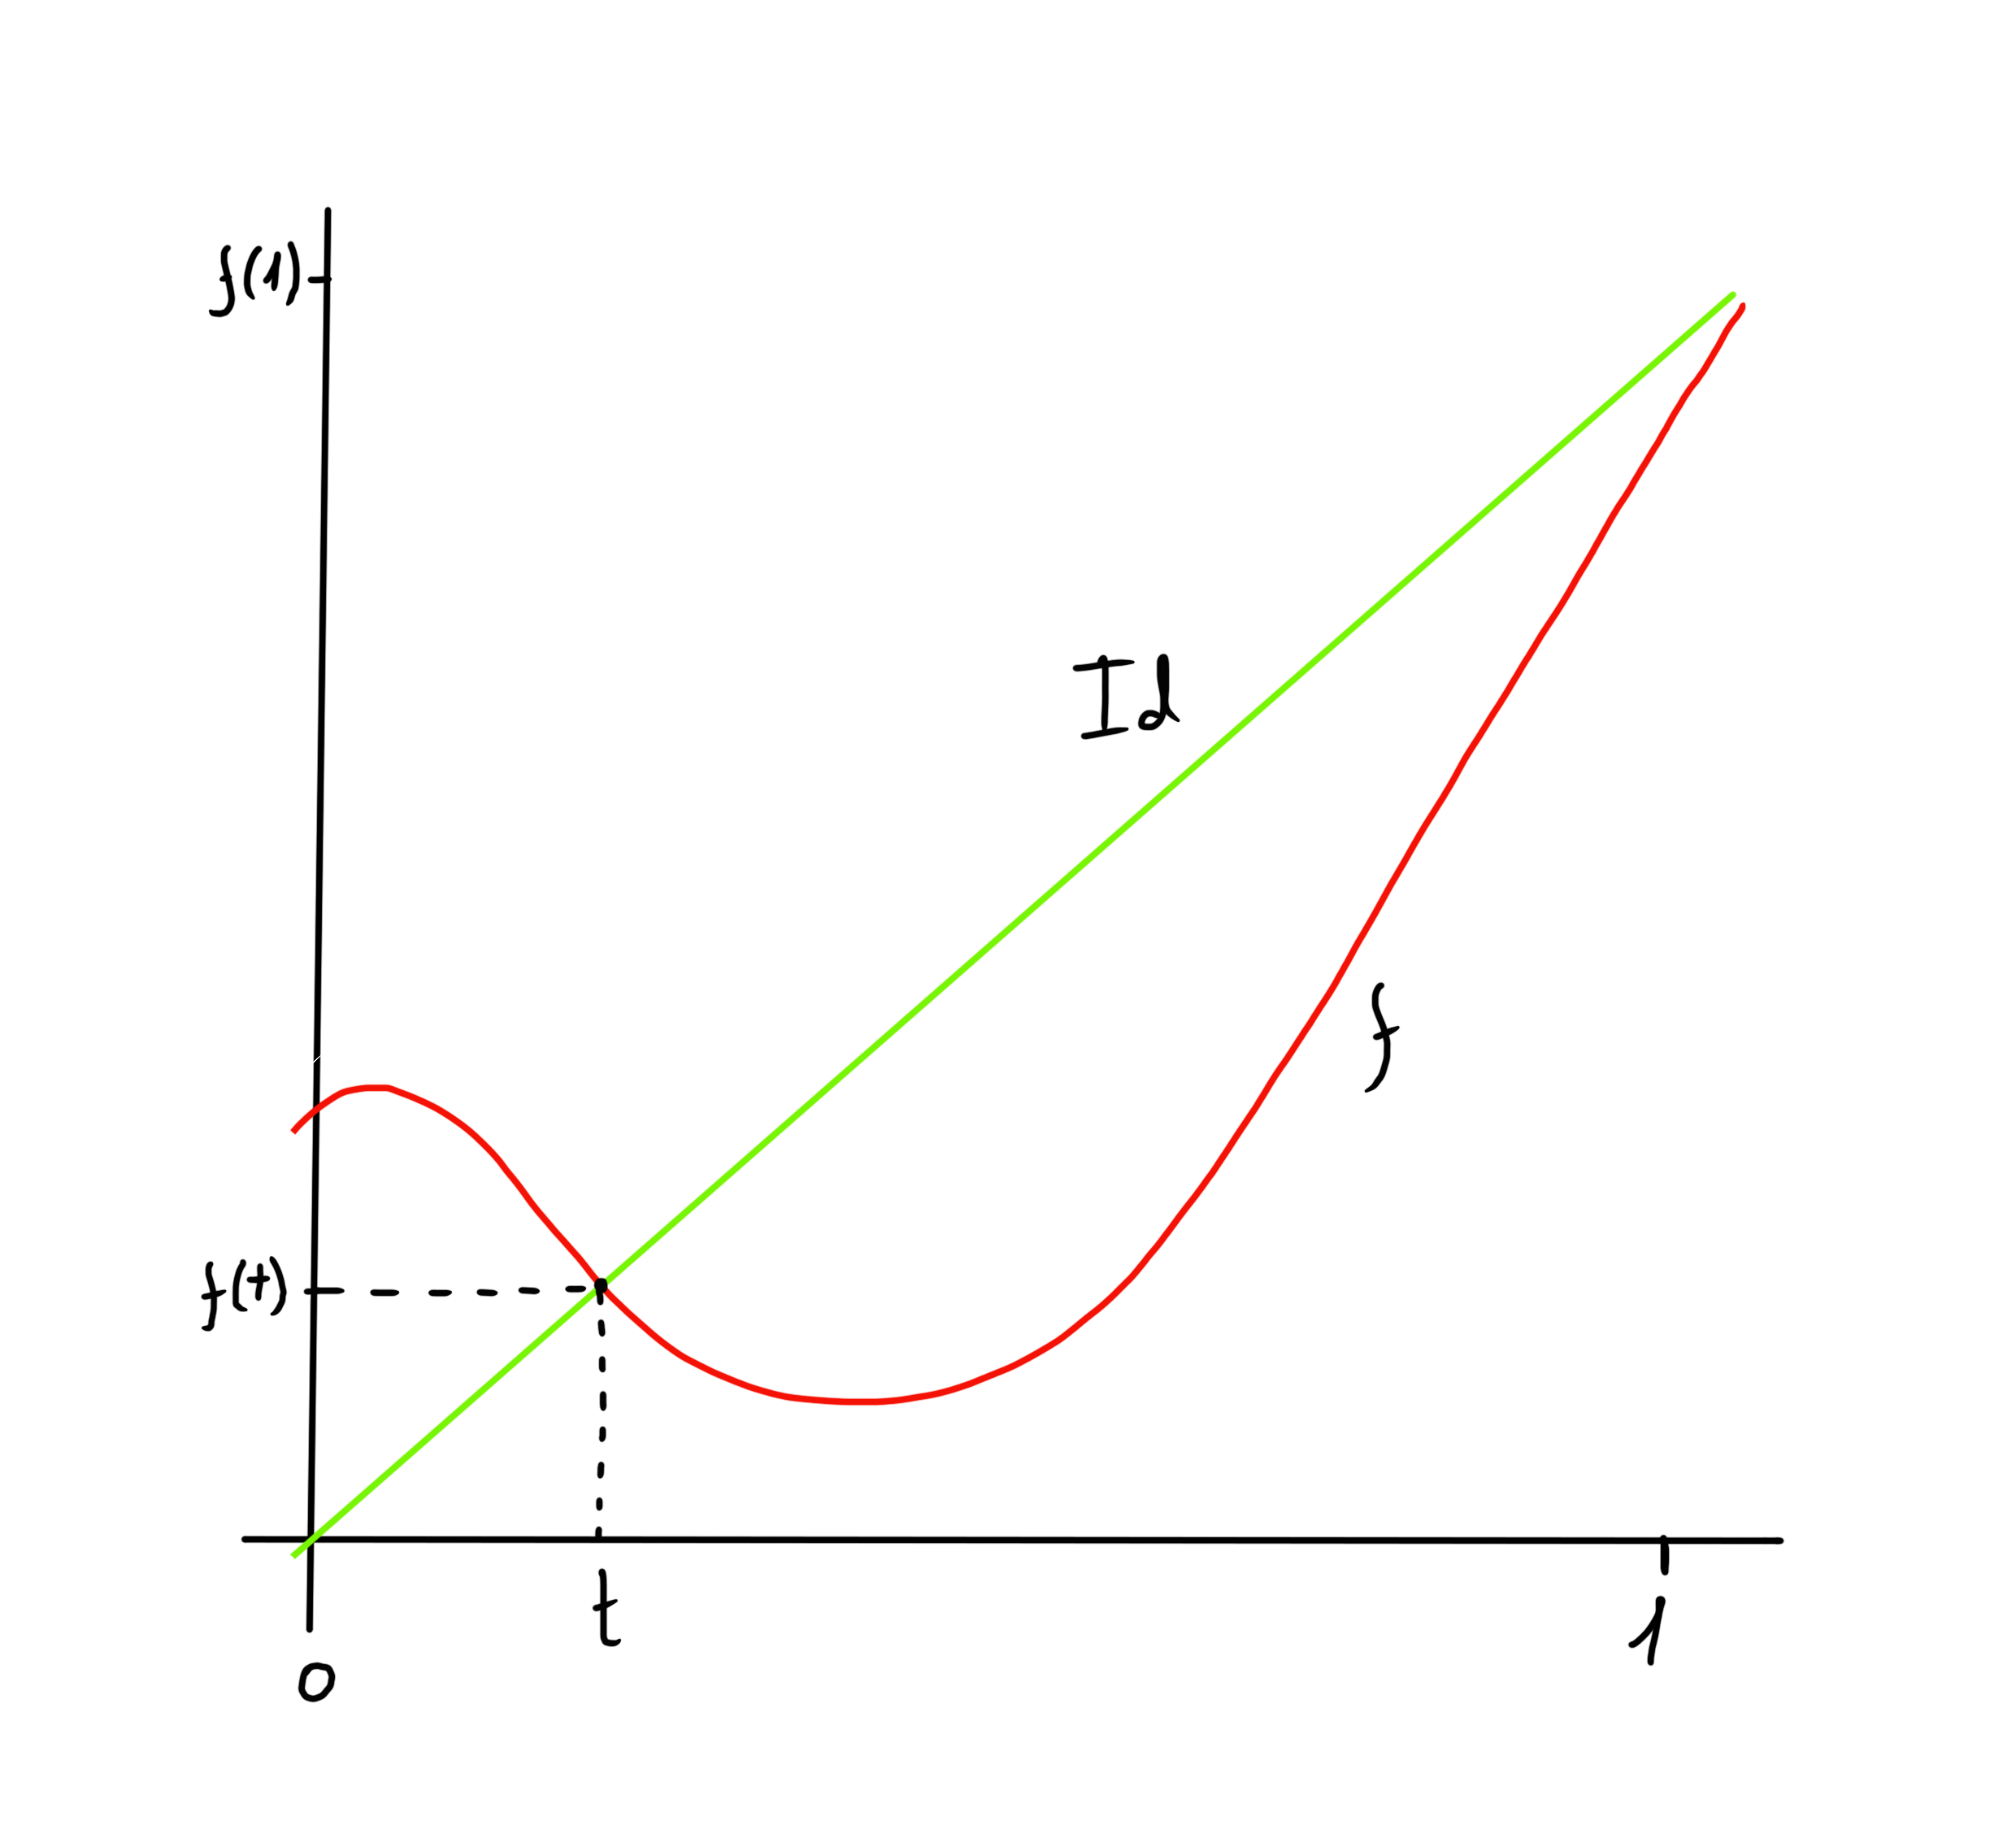
\includegraphics[scale=0.08]{unnamed.PNG}
\caption{En la figura se puede observar el punto fijo $(t,f(t))$, y que en la aplicación $Id$ todos los puntos son fijos.}
\end{center}
\label{fig:4}
\end{figure}
\end{sol}
\end{ejern}

\end{ejern}
\begin{ejern} \textbf{96.} Sea $X$ un espacio topológico cualquiera y $f : [0, 1] \longrightarrow X$ una aplicación continua. Deduce que $f(0)$ y $f(1)$ están en la misma componente conexa de $X$.
\begin{sol}
Sabemos que $f(0) \in f([0,1])$ y que $f(1) \in f([0,1])$, y que cada uno está en una componente conexa, digamos $C_{f(0)}$ y $C_{f(1)}$. De forma que $C_{f(0)} \cap C_{f(1)} \neq \emptyset$, por lo tanto como dos componentes conexas o son disjuntas o son la misma, y no son disjuntas, pues son la misma ($C_{f(0)}= C_{f(1)}$)
\end{sol}
\end{ejern}

\begin{ejern} \textbf{97.}
Calcula las componentes conexas de ($\mathbb{R}, \mc{T}_{inf}$) donde $\mc{T}_{inf}$ es la topología de límite inferior o de Sorgenfrey, que es generada por la base de abiertos $\beta=\{[a,b) \: / \: a,b \in \mathbb{R}, a < b \}$
\end{ejern}
\; \vspace{-5mm}
\begin{ejern} \textbf{99. }
\begin{enumerate}[a)]
    \item Probar que $\mathbb{R}^n - \{0\}$ es conexo para todo $n \geq 2$
    \begin{sol}
    Veamos que $\mathbb{R}^n$ es conexo si $n>1$. Para $n=1$, si quitamos un punto a la recta real, podemos ver que no es conexo. Veamos que $\mathbb{R}^2 - \{p\}$ es conexo por caminos, y por lo visto en \hyperref[cpc]{\textcolor{blue}{\textbf{7.7. Subconjuntos conexos por caminos}}}, conexo.
    
    Sean $x,y \in \mathbb{R}^2$, definimos el camino $\varphi$ :
    $$\begin{array}{rcl}
         [0,1] & \stackrel{\varphi}{\longrightarrow} & \mathbb{R}^n \\
         t & \longmapsto & xt+(1-t) \: y 
    \end{array}$$
    que empieza en $y$ y acaba en $x$, de forma que obtenemos un segmento $r$, si $p \nin r$. Si se diera el caso de que que $p \in r$, escogeríamos otro punto $z$, de forma que el camino de $x$ a $y$ sea una composición de los caminos de $x$ a $z$ y de $z$ a $y$. 
    
    De esta forma, podemos escoger $n$ mayores, obteniendo el mismo resultado, de forma que se demuestra
    \end{sol}
    \item Probar que $\mathbb{R}$ y $\mathbb{R}^n$ no son homeomorfos si $n \neq 1$.
    \begin{sol}
    Sea $\varphi$ el homeomorfismo:
    $$\begin{array}{rcl}
        \mathbb{R} & \stackrel{\varphi}{\lower 2.5pt \hbox{$\widetilde{\vrule width 20pt height 3.9pt depth -3.5pt}$}} & \mathbb{R}^n \\
        p & \longmapsto & q
    \end{array}$$
    Como hemos visto en el ejercicio anterior, $\mathbb{R} - \{p\}$ no es conexo, y por el homeomorfismo, se la asigna $\mathbb{R}^n-\{q\}$, que por lo visto anteriormente, \underline{sí} es conexo, lo cual es una contradicción, ya que dos espacios homeomorfos y uno es conexo, el otro tambi{\'e}n lo es.
    \end{sol}
    \item Sea $p \in S^1$, probar que $S^1 - \{p\}$ es conexo, y deducir que $S^1$ no es homeomorfo a $\mathbb{R}$.
    \begin{sol}
    Se define $S^1:=\{x \in \mathbb{R}^2 \: / \: ||x|| = 1 \}$, de forma que es conexo por caminos, análogamente a lo visto en \textit{a)}, por tanto conexo (además de ser $S^1$ homeomorfo a $\mathbb{R}^2$), por lo que igual que en \textit{b)}, $S^1- \{p\}$ no es homeomorfo a $\mathbb{R} - \{q\}$. 
    \end{sol}
\end{enumerate}
\end{ejern}
\; \vspace{-5mm}
\begin{ejern} \textbf{104.} Estudiar la conexión, conexión local y conexión por caminos en ($X,\mc{T}$) con la topología del punto incluido $T = \{U \subseteq X \: / \: p \in  U\} \cup \{\emptyset\}$.
\end{ejern}
\begin{sol}
Vemos si $(X, \mc{T})$ es conexo por caminos (y por tanto, conexo). Sea $X \ni q \neq p$, veamos si existe la aplicación continua $\gamma: [0,1] \longrightarrow X$ tal que $\gamma(1)=q$ y $\gamma(1)=p$. Definimos la aplicación de forma que  se cumple que $\left\{ \begin{array}{l}
     \gamma(1)=q  \\
     \gamma([0,1))=p 
\end{array} \right.$

Veamos que $\gamma$ es continua. Dado un abierto $U \in X$, $\gamma^{-1}(U)=\left\{ \begin{array}{l}
     [ 0 , 1 )  \text{ si } q \nin U  \\
     \left[ 0 , 1 \right] \text{ si } q \in U
\end{array} \right.$ 

Podemos observar que ambos son abiertos en [0,1], [0,1] por ser el total y [0,1) por ser la intersección [0,1] con un abierto de $\mathbb{R}$ (por ejemplo, (-1,1) $\cap$ [0,1]). Por lo tanto, se comprueba que $\gamma$ es continua y que por lo tanto, $(X,\mc{T})$ es conexo por caminos y a su vez, conexo. 

Veamos que es localmente conexo. Por definición, si es localemnte conexo existe una base de abiertos coexos. Sean $U, V \subseteq X$ dos abiertos, $U \cap V \neq \emptyset$ son disjuntos, por ser $X$ irreducible. Entonces todo abierto de $X$ es conexo y por lo tanto, $X$ localmente conexo.
\end{sol}
\; \vspace{-5mm}
\begin{ejern} \textbf{105.} Estudiar la conexión, conexión local y conexión por caminos en ($X,\mc{T}$) con la topología del punto excluído $T = \{U \subseteq X \: / \: p \nin  U\} \cup \{X\}$.
\end{ejern}
\begin{sol}
Al igual que en el ejercicio anterior, en primer lugar estudiaremos la conexión por caminos. Veamos la aplicación $\gamma$ tal que $\gamma(1)=p$ y $\gamma([0,1)) = q$. Veamos que es continua.

Dado un abierto $U \in X$, $\gamma^{-1}(U)=\left\{ \begin{array}{l}
     [ 0 , 1 )  \text{ si } q \in U  \\
     \emptyset  \text{ si } q \nin U
\end{array} \right.$

Por lo visto en el ejercicio anterior, ambos son abiertos, y por lo tanto, $\gamma$ es continua y por ello, $(X, \mc{T})$ conexo por caminos y conexo. 

Veamos su conexión local. Sea $x \in X$, \vspace{-5mm}
\begin{itemize}
    \item Si $x \neq p$, entonces $\{x\}$ es abierto y conexo, con $x \in \{x\}$
    \item Si $x = p$, entonces existe un entorno de $p$, que contiene a un abierto conexo $U$ tal que $p \in U$. Por lo tanto, $U=X$ ya que es el {\'u}nico abierto conexo que contiene a $p$, y por lo tanto, concluimos que no es localmente conexo. 
\end{itemize}
\end{sol} 
\begin{ejern} \textbf{106.}
 Si $X$ es infinito y numerable, estudiar la conexión, conexión local y conexión por caminos de ($X, \mc{T}_{CF}$) con la topología cofinita. (\textit{Observación.} No es metrizable)
\end{ejern}
\begin{sol}
Recordemos que la topología cofinita es $\mc{T}_{CF}=\{U\: / \: X-U \text{ es finito o vacío }\}$. Como $X$ es infinito y numerable, existen cualesquiera abiertos $U,V \subseteq X$ son disjuntos ($U \cap V \neq \emptyset$), y por lo tanto, todo abierto es conexo ($X$ incluido). Concluyendo así que es localmente conexo y conexo.

Veamos su conexión por caminos. Definamos la aplicación continua $\gamma: [0,1] \longrightarrow X$. Como $X$ es numerable y los puntos son cerrados (por ser su complementario infinito), podemos obtener una familia numerable de cerrados en [0,1]: $\Big\{ \gamma^{-1}(x) \Big\} _{x\in X}$ donde identificaremos cada $C_i = \gamma^{-1} (x_i)$. Por lo tanto, podemos expresar el intervalo [0,1] = $\underset{i \in \mathbb{N}}{\mathlarger{\bigsqcup \;}} \: C_i$, es decir, como unión disjunta de cerrados 2 a 2, y por lo tanto, como unión de conjuntos finitos de puntos, de forma que nos permite expresar [0,1] = $\underset{i}{\mathlarger{\bigsqcup \;}} \{x_1^i, \ldots x_r^i\}$. Es decir, que el intervalo [0,1] es numerable, llegando a una contradicción y concluyendo que no es conexo por caminos. 
\end{sol}
\;
\section{Compacidad} \vspace{-15mm} \hfill \footnote{\url{https://studium.usal.es/pluginfile.php/761363/mod_resource/content/0/Cap5-Compactos.pdf}}

\textit{Definición.} Sea $A \subset (X, \mc{T})$ un subespacio, diremos que es compacto si $(A, \mc{T}_{|_A})$ es un espacio topológico compacto. 
\; 
\begin{ejern} \textbf{111.} Probar que la compacidad es una propiedad absoluta, en el sentido de que para ver si $A \subseteq (X, \mc{T})$ es compacto basta con estudiar los recubrimientos de $A$ por abiertos de $(X, \mc{T})$.
\end{ejern}
\begin{sol} Lo podemos expresar como sigue:

$(A, \mc{T}_{|_A})$ es compacto $\Leftrightarrow$  $\mathlarger{\exists} $ un recubrimiento $ \underset{i \in I}{{\mathlarger{\bigcup}}} \: U_i \supset A $ con $U_i \in \mc{T}$ tal que hay un subrecubrimiento $ \overset{k}{\underset{j=1}{\mathlarger{\bigcup}}} \: U_{ij}  \supset A$

$\Rightarrow)$ Sea $(A, \mc{T}_{\: |_A})$ compacto y $\{U_i\}_{i \in I}$ una familia de abiertos de $(X, \mc{T})$ tal que $A \subset  \underset{i \in I}{{{\bigcup}}} \: U_i$, entonces $A= \underset{i \in I}{\bigcup}(U_i \cap A)$ donde cada $U_i \cap A$ es un abierto de $(A, \mc{T}_{\:|_A})$. Por lo tanto, existe $J \subset I$ finito tal que $A=\underset{J}{\bigcup}\: (U_j \cap A)$, cumpli{\'e}ndose que $A \subset \underset{j \in J}{\bigcup} \: U_j$.

$\Leftarrow)$ Sea $A=\underset{i \in I}{\bigcup} \: V_i$ con $\{V_i\}_{i \in I}$ una familia de abiertos de $(A, \mc{T}_{\:|_A})$, $V_i=U_i \cap A$ para alg{\'u}n $U_i \in \mc{T}$. Entonces $A=\underset{i \in I}{\bigcup} \: U_i \cap A \; \subset \underset{i \in I}{\bigcup} \: U_i$. Podemos asegurar que $\mathlarger{\exists} J \subseteq I$ finito tal que $A \subset \underset{j \in J}{\bigcup} \: U_j$, y por lo tanto $A=  \underset{j \in J}{\bigcup} \: U_j \cap A = \underset{j \in J}{\bigcup} \: V_j$.
\end{sol}
\; \vspace{-5mm}
\begin{ejern} \textbf{113.}
Si un espacio topológico $(X, \mc{T})$ es compacto ¿lo es necesariamente con una topología $\mc{T}'$ menos fina, $\mc{T}' \leq \mc{T}$? ¿Qu{\'e} se puede decir en ambos casos de ($X, \mc{T}'$) sabiendo que
($X, \mc{T}$) no es compacto?
\end{ejern}
\begin{sol} \; \vspace{-7mm}
\begin{itemize}
    \item Sea $(X,\mc{T})$ compacto $\Rightarrow$ $(X,\mc{T}')$ tambi{\'e}n es compacto.
    
     Sean $U_i' \in \mc{T}'$, entonces $U_i' \in \mc{T}$. Y, por ser $(X, \mc{T})$ compacto, existe un recubrimiento $X=\underset{i \in I}{\bigcup} U_i '$, y por lo tanto, $(X, \mc{T}')$ es compacto.
     
     \item Sea $(X,\mc{T})$ no compacto, entonces $(X, \mc{T}')$ con $\mc{T}' \leq \mc{T}$ puede ser compacto o no.
     
     Sea $\mc{T}'=\mc{T}_{trivial} \Rightarrow (X, \mc{T}')$, $\mc{T}'=\{\emptyset, X\}$. Sea $U$ un recubrimiento abierto de $X$, entonces $X \in U$, por lo que $\{X\}$ es un subrecubrimiento de $X$, por lo que $(X, \mc{T}_{trivial})$ es compacto. 
     
     \item Dadas dos topologías no compactas (que generan espacios no compactos), veamos que el hecho de que $(X,\mc{T}')$ no sea compacto implica que $(X,\mc{T})$ para $\mc{T}' \leq \mc{T}$.
     
     Veamos un ejemplo. Sea $\mc{T}'=\mc{T}_{usual}$ y $\mc{T}=\mc{T}_{inf}$, donde $\mc{T}_{usual} \leq \mc{T}_{inf}$. Los espacios $(\mathbb{R},\mc{T}_{usual} )$ y $(\mathbb{R},\mc{T}_{inf} )$ no son compactos. Veamos la implicación. $\mathbb{R} = \underset{n \in \mathbb{N}}{\bigcup}(-n,n) \neq (-m,m)$ donde $m=\max\{|n_i|\}$ con $i \in J$ finito. Con la otra topología, $\mathbb{R}=\underset{n \in \mathbb{N}}{\bigcup}[-n,n) $ es un recubrimiento por abiertos, pero que no admite subrecubrimientos finitos. Se puede ver que ambos no son compactos.
\end{itemize}
\end{sol}
\; \vspace{-5mm}
\begin{ejern} \label{ej114} \textbf{114.} Probar que todo subconjunto finito de un espacio topológico es compacto. 
\end{ejern}
\begin{sol}
Basta probar que todo espacio topológico finito es compacto. 

Sea $(X, \mc{T})$ un espacio topológico con $|X|$ finito, ($X, \mc{T}$) es compacto. Sea $|X|=n \; \Rightarrow |\mc{P}(X)| = 2^n$, luego todo recubrimiento es finito, obviando las repeticiones de abiertos. 
\end{sol}
\; \vspace{-5mm}
\begin{ejern} \textbf{115.} Sea $X$ un espacio discreto,
\vspace{-5mm} \begin{center}
    $X$ es compacto $\Leftrightarrow$ $X$ es finito.
\end{center}
\end{ejern}
\begin{sol}\; 

$\Leftarrow$) Se ha demostrado en el ejercicio anterior. 

$\Rightarrow$) Sea $X$ discreto, $\big\{\{x\}\big\}_{x \in X}$ es un recubrimiento por abiertos de $X$, es decir,\\ $X=\underset{x \in X}{\bigcup}\{x\}$. Por ser $X$ compacto, existen $x_1, \ldots, x_r \in X$ tales que $X=\overset{r}{\underset{i=1}{\bigcup}} \{x_i\}$ y por lo tanto, $X$ es finito.
\end{sol}
\; \vspace{-5mm}
\begin{ejern} Sea $\{x_n\}$ una sucesión en $X$ tal que  $\exists \; x \in \lim x_n$, probar que $Y=\{x_n\}_{x \in \mathbb{N}} \cup \{x\}$ es compacto en $(X, \mc{T})$.
\end{ejern}
\begin{sol}
Sea $\{U_i\}_{i \in I}$ un recubrimiento de $Y$ por abiertos, 
$$x \in \lim x_n \Rightarrow \; \forall \: U_x \text{ entorno de } x \; \exists \; n_0 \in \mathbb{N} \; / \; \forall n > n_0 \text{ cumple que } x_n \in U_x $$
Por lo tanto, existe un $i_0 \in I$ tal que $x \in U_{i_0}$. Por lo tanto, $\exists \; n_0 \in \mathbb{N} \; / \; \forall n > n_0$  cumple que  $x_n \in U_{i_0}$. Tomando $U_{ij}$ con $x_j \in U_{i_j}$ para todo $0 < j < n_0$. Por lo tanto, $U_{i_0} \cup U_{i_1} \cup \ldots \cup U_{n_0 -1} = Y$, donde $x_{n_0}, x_{n_0 +1}, \ldots, x_n \in U_{i_0}$.
\end{sol}




\chapter{ANEXO: PARCIAL 2020-21}
\begin{center}
    \textbf{\underline{TEORíA}}
\end{center}
1. Definir, con todo rigor, los siguientes conceptos:
\begin{enumerate}[1)]
    \item Topología (por abiertos) en un conjunto $X$.
    \item Aplicación continua entre espacios topológicos.
    \item Punto de adherencia de un subconjunto $S$ de un espacio topológico $X$.
    \item Topología producto de $X \times Y$ (siendo $X$ e $Y$ espacios topológicos).
    \item Topología inicial de una aplicación.
    \item Topología final de una aplicación. 
    \item Espacio topológico $T_0$.
    \item Espacio topológico $T_1$.
    \item Espacio topológico $T_2$.
    \item Espacio topológico conexo.
    \item Componente conexa de un espacio topológico.
    \item Espacio topológico conexo por caminos.
    \item Producto o composición de dos cominos.
    \item Caminos homótopos.
    \item Grupo fundamental de un espacio topológico $X$ en un punto $p$.
\end{enumerate}
\begin{center}
    \textbf{\underline{PROBLEMAS}}
\end{center}
2. Sea $X$ un conjunto y $A \subseteq X$ un subconjunto. Se define una topología en $X$ como 
$$\mc{T}_X=\{ U \subseteq X \; : \; A \subseteq U\} \cup \{ \emptyset \}$$
\begin{enumerate}[(a)]
    \item Probar que $\beta=\{ \{ x \} \cup A \; : \; x \in X \}$ es una base de $\mc{T}_X$.
    \item Si $B \subseteq X$, hallar el interior, el exterior y el cierre de $B$.
    \item ¿Qué topología induce $\mc{T}_X$ en $A$?
\end{enumerate}
3. Sea ($X, \mc{T}$) un espacio topológico. Para cada $x \in X$ denotamos por $E(x)$ a la familia de todos los abiertos de $x$. Para cada subconjunto $Y$ de $X$ denotamos $\mc{T}_{|_Y}$ a la topología inducida por $\mc{T}$ en $Y$. Probar que $$\{x\} = \underset{V \in E(x)}{\mathlarger{\bigcap}} V, \text{ para todo } x \in X \; \Longleftrightarrow \; \mc{T}_{|_F} \text{ es la discreta, para todo } F \subset X \text{ finito.}$$
\textit{Indicaciones}
\vspace{-3mm}
\begin{enumerate}[(a)]
    \item Probar que $\{x\} = \underset{V \in E(x)}{\mathlarger{\bigcap}} V, \text{ para todo } x \in X \; \Longleftrightarrow \; \{x\} $ es cerrado, para todo $x \in X$.
    \item Si para cada subconjunto $Y$ de $X$ denotamos $Y^a$ al conjunto de puntos aislados de $Y$, probar que la topología inducida por $\mc{T}$ en $Y$ es la discreta si y sólo si $Y=Y^a$
    \item Concluir que $\{x\} $ es cerrado, para todo $x \in X$, si y solo si para todo $F$, subconjunto finito de $X$, todo punto $y \in F$ es abierto en ($F,  \mc{T}_{|_F}$)
\end{enumerate}

\begin{center}
\Huge{RESOLUCIóN}\\
\normalsize \; \\
    \textbf{\underline{TEORíA}}
\end{center}
\begin{enumerate}[1)]
    \item Topología (por abiertos) en un conjunto $X$. \textcolor{blue}{\ref{def:abierto}.} \\ 
    \item Aplicación continua entre espacios topológicos. \textcolor{blue}{\ref{def:conti}.} \\ Sean los espacios topológicos $(X, \mc{T}_X)$ e $(Y, \mc{T}_Y)$, una aplicación $f: X \longrightarrow Y$ es continua si la antiimagen de cualquiera abierto de $Y$ es un abierto de $X$, es decir: 
    $$\text{Si } U\in \mc{T}_Y \text{, entonces } f^{-1}(U) \in \mc{T}_X$$
    \item Punto de adherencia de un subconjunto $S$ de un espacio topológico $X$. \textcolor{blue}{\ref{sec:adherencia}.} \\
    Diremos que $x \in X$ es un punto adherente al subconjunto $S$ (en $X$) si todo abierto de $X$ que contenga a $x$ corta a $S$. Es decir, sea $U$ un abierto cualquiera, entomces $U \cap A \neq \emptyset$.
    \item Topología producto de $X \times Y$ (siendo $X$ e $Y$ espacios topológicos). \textcolor{blue}{\ref{sec:producto}.}\\ 
   El producto en $X \times Y = \{ (x,y), \: x \in X, \: y \in Y \}$ define la topología inicial de $\pi_X, \: \pi_Y$. Los abiertos de $X \times Y$ son: 
    $$\pi^{-1}_X (U)=U \times Y \text{ y }\pi^{-1}_Y (V)=X \times V $$
    siendo $U$ y $V$ abiertos de $X$ e $Y$, respectivamente. La intersección de lo anterior es $U \times V$, que es un abierto de $X \times Y$. Como ya se sabe, todo abierto de $X \times Y$ es unión de abiertos del tipo $U \times V$.
    \item Topología inicial de una aplicación. \textcolor{blue}{\ref{sec:topi}.} \\
    Sea $f: X \longrightarrow Y$ una aplicación donde $X$ es un conjunto e $Y$ es un espacio topológico, un subconjunto $U$ de $X$ es abierto si existe un $V \subseteq Y$ tal que $U=f^{-1}(V)$ para alg{\'u}n $V$ abierto. Es la mínima topología en $X$ tal que $f$ es continua.
    \item Topología final de una aplicación. \textcolor{blue}{\ref{sec:topf}.} \\ 
    Sea $f: X \longrightarrow Y$ una aplicación donde $X$ es un espacio topológico e $Y$ es un conjunto, un subconjunto $V$ de $Y$ es abierto si $f^{-1}(V)$ es un abierto. Es la máxima topología en $Y$ tal que $f$ es continua.
    \item Espacio topológico $T_0$. \textcolor{blue}{\ref{espt0}.}\\
    Un espacio topológico es $T_0$ o separado si para toda pareja de puntos $x,y$ pertenecientes al espacio, podemos encontrar un abierto que contenga a uno y no a otro.
    \item Espacio topológico $T_1$. \textcolor{blue}{\ref{espt1}.}\\
    Un espacio topológico es $T_1$ si para toda pareja de puntos $x,y$ podemos encontrar un par de abiertos que contienen a cada punto ($U_x, U_y$ tal que $x \in U_x$ e $y \in U_y$) pero que no contienen al otro.
    \item Espacio topológico $T_2$. \textcolor{blue}{\ref{espt2}.} \\
    Un espacio topológico es $T_2$ si para cualquier pareja de puntos $x,y$ podemos encontrar un par de abiertos $U_x,U_y$ que contengan cada uno a un punto y no al otro, y además, sean disjuntos ($U_x \cap U_y = \emptyset$)
    \item Espacio topológico conexo. \textcolor{blue}{\ref{conexo}.}\\
    Diremos que un espacio topológico $X$ es conexo si no es unión de dos abiertos no vacíos y disjuntos, es decir, si para si $X$ es unión de dos abiertos, estos o son vacíos o no son disjuntos (se cortan).
    \item Componente conexa de un espacio topológico. \textcolor{blue}{\ref{ccon}.}\\
    Una componente conexa $C_x$ de un espacio topológico $X$ es un subconjunto que contiene a un punto $x \in X$ y es maximal. Esto es, que no existe un subconjunto mayor, o que todo subconjunto que contenga a $x$ está contenido en $C_x$.
    \item Espacio topológico conexo por caminos.  \textcolor{blue}{\ref{cpc}.} \\
    Se dice que un espacio topológico es conexo por caminos si para toda pareja de puntos $p,q \in X$ existe una aplicación $\gamma: [0,1] \longrightarrow X$ que llamaremos camino tal que $\gamma(0)=p$ y $\gamma(1)=q$
    \item Producto o composición de dos caminos. \textcolor{blue}{\ref{compcam}.} \\
    Se define el producto o composición de dos caminos $\gamma, \gamma'$ tales que $\gamma(1)=\gamma'(0)$ (es decir, el final de uno, es el inicio del siguiente) de la siguiente manera:  \\
    $\gamma \cdot \gamma'(t)=\gamma(2t)$ si $t\in [0,\nicefrac{1}{2}]$ y $\gamma \cdot \gamma'(t)=\gamma'(2t-1)$ si $t\in [\nicefrac{1}{2},1]$.
    \item Caminos homótopos. \textcolor{blue}{\ref{camhom}.}  \\
    Diremos que dos caminos $\gamma, \gamma'$ son homtótopos si existe una aplicación $H$ tal que:
    \begin{itemize}
        \item $H(s,0)=\gamma (s) $
        \item $H(s,1)=\gamma' (s) $
        \item $H(0,t)=p$
        \item $H(1,t)=p$
    \end{itemize} 
    Es decir, que tienen el mismo inicio y final y existe una aplicación que deforma uno en el otro.
    \item Grupo fundamental de un espacio topológico $X$ en un punto $p$. \textcolor{blue}{\ref{grupfun}.}  \\
    Definimos el grupo fundamental de un espacio $X$ en un punto $p$ (con base $p$) como el conjunto cociente de los lazos con base $p$ con las homotopías entre lazos tal que $\ell \: \sim \: \ell'$. Lo denominaremos $\mathlarger{\mathlarger{\pi_1}}(X,p)$.
\end{enumerate}

\begin{thebibliography}{X}
    \bibitem{Mun} \textsc{Munkres, James R.}
        \textit{Topología}. 2ª edición, 2002. ISBN: 84-205-3180-0.
\end{thebibliography}

\end{document}

%%Recordatorio para la inutil de Sara que no sabia que se hace asi \textbf{\textcolor{blue}{\hyperref[dempito]{8.3. Componentes conexas}}}.%%
%% Para saber como se pone esto:
\xymatrix{
E \ar[r]^{D} \ar[rd]^{\:} & E \ar[d]^{\omega_0} \\
&k
} 



